\documentclass{article}
\input{setup.tex}

\usepackage{soul}
\usepackage{accents}
\usepackage{quiver}
\usepackage{spectralsequences}

\renewcommand*\contentsname{Table of Content}

\title{MATH 6180 Fall 2024 Notes}
\author{Mattie Ji}
\date{Updated \today}
\setlength\parindent{0pt}

\begin{document}

\maketitle
These are lecture notes from \textbf{MATH 6180: Algebraic Topology Part I} (this is really Part II) with Professor Jonathan Block at the University of Pennsylvania for the Fall 2024 semester.\\

These notes are taken by Mattie Ji with gracious help and input from the instructor of this course. If you find any mistakes in these notes, please feel free to direct them via email to me or send a pull request on GitHub. The notes are last updated \today.

\tableofcontents

\newpage

\section{Lecture August 27th, 2024}

\subsection{Introduction}

This class is called \textbf{MATH 6180: Algebraic Topology}. This is a year-long sequence about advanced topics in algebraic topology. The name of the class is poorly phrased because it is really a second course to algebraic topology(or some might argue even a third course).\\

\textbf{Question:} As customary for every class, we must ask the question - what is algebraic topology? There are two interpretations.
\begin{enumerate}
    \item Algebra in service to topology. Here we have subjects like manifold theory.
    \item Topology in service of algebra. Here we have subjects like algebraic K-theory and higher category theory.
\end{enumerate}

\begin{remark}
    ``Derived categories are really homotopy theory" - exclaimed by the instructor.
\end{remark}

We will be covering both parts in this sequence. We won't have an official textbook for the course, but the following references would be quite useful:
\begin{enumerate}
    \item Hatcher, Algebraic Topology, free on Allen Hatcher's website.
    \item Bott and Tu, Differential Forms in Algebraic Topology.
    \item Strom, Modern Classical Homotopy Theory.
    \item Switzer, Algebraic Topology, Homology, and Homotopy Theory.
\end{enumerate}
We will be adding more to this list as the course goes on.\\

The instructor will try to hand out homework problems once a week, but realistically it will be once every other week. You will be only graded on the homework and possible presentation of the homework problems, but no exams.\\

\textbf{Pre-requisites:}
\begin{enumerate}
    \item Homology, Cohomology (Partial), \st{Poincare Duality}
    \item Categorical Language (Category, Functor, Limit and Co-limits)
    \item Fundamental Group and Covering Space
\end{enumerate}

\subsection{Course Syllabus and Outline}

The outline of the course for \textbf{\ul{this semester}} is currently as follows.
\begin{enumerate}
    \item Homotopy Theory
    \begin{itemize}
        \item A. Homotopy of maps, homotopy equivalence, homotopy groups, Whitehead's theorem, Cellular Approximation, CW-approximation
        \item B. Calculations, Blakers-Massey Theorem (excision in homotopy theory), Freudenthal Suspension Theorem, Hurewicz Theorem
    \end{itemize}
    A big emphasis for this part is to find a ``good classes of spaces and maps" to do homotopy theory.
    \begin{itemize}
        \item Cofibrations are a kind of maps that behaves well with respect to homology. (A quintessential example is the inclusion of a decent closed set into a bigger space). On the other hand, homotopy does not behave well with respect to cofibirations.
        \item Homotopy groups work very well with respect to fibrations. Homology does not work very well with cofibrations.
    \end{itemize}
    \item Fiber Bundles and Fibrations
    \begin{itemize}
        \item A. Homotopy Lifting Property and fibrations, LES of homotopy groups from a fibration
        \item B. Fiber bundles are fibrations
        \item C. Structure fiber bundles (adding a topological group to the fiber bundle), principal G-bundles
        \item D. Homotopy classification of fiber bundles, classfying spaces
    \end{itemize}
    \item Spectral Sequences
    \item Characteristic Classes - Steifel-Whitney, Chern, Pontryagin classes\\

    Characteristic classes provide ways to show that two homotopy equivalent spaces are not homeomorphic (or diffeomorphic).
\end{enumerate}

Here are somethings this class would not cover, but one of you might want to talk about it:
\begin{enumerate}
    \item H-cobordism theorem (a criterion for two manifolds to be diffeomorphic):
    \begin{theorem}
        Suppose $W^{n+1}$ is a compact, simply connected, differentiable manifold with $n \geq 5$ whose boundary $\partial W = M_1 \sqcup M_2$ for $M_1, M_2$ are two differentiable compact $n$-manifolds. Suppose that for $i = 1, 2$ the inclusion $M_i \to W$ is a homotopy equivalence, then $W$ is diffeomorphic to $M_1 \times [0, 1]$. This in particular implies that $M_1$ and $M_2$ are diffeomorphic.
    \end{theorem}
    \item Reidemeister Torsion - this was specifically invented to classify all $3$-dimensional Lens space. There are actually Lens spaces that are diffeomorphic but not homotopy equivalent, and the Reidermeister torsion provides a good example of invariants that can tell homotopy equivalent Lens spaces apart.
\end{enumerate}

\begin{definition}
    A map $\rho: Y \to X$ is a fiber bundle if for all $x \in X$, there exists $U \subseteq X$ open such that there exists a homeomorphism $\varphi: \rho^{-1}(U) \to U \times F$ such that the following diagram commutes
    % https://q.uiver.app/#q=WzAsMyxbMCwwLCJcXHJob157LTF9KFUpIl0sWzEsMCwiVSBcXHRpbWVzIEYiXSxbMCwxLCJVIl0sWzAsMiwiXFxyaG8iXSxbMCwxLCJcXHZhcnBoaSIsMl0sWzEsMl1d
\[\begin{tikzcd}
	{\rho^{-1}(U)} & {U \times F} \\
	U
	\arrow["\varphi"', from=1-1, to=1-2]
	\arrow["\rho", from=1-1, to=2-1]
	\arrow[from=1-2, to=2-1]
\end{tikzcd}\]
\end{definition}

Office hour is by appointment (email). If the door is open, you are welcome to walk in, but you might get rejected.

\newpage
\section{Lecture August 29th, 2024}

\subsection{The Spaces We Are Working With}

We want a class of spaces which is well behaved and contain the spaces that we care about. Here are some properties we want the class to satisfy:
\begin{enumerate}
    \item The collection should contain manifolds, algebraic and complex varieties, $CW$ complexes.
    \item The space should be closed under certain constructions. 
    \item These constructions should be well-behaved.
\end{enumerate}

\begin{example}
    Here are some example of spaces that we consider to be nice and want to work with.
    \begin{itemize}
        \item (0) $*$ - a point.
        \item (1) $\mathbb{S}^n = \{x \in \Rbb^{n+1}\ |\ |x| = 1\}$.
        \item (2) $\mathbb{D}^{n+1} = \{x \in \Rbb^{n+1}\ |\ |x| \leq 1\}$. Note that $\mathbb{S}^n = \partial \mathbb{D}^{n+1}$.
        \item (3) $\Cbb P^{n} = \frac{\Cbb^{n+1} - \{0\}}{\Cbb^{\times}}$. Here the $\Cbb^{\times}$ action on $\Cbb^{n+1} - \{0\}$ is given by
        \[\lambda \cdot (z_0, ..., z_n) = (\lambda z_0, ..., \lambda z_n).\]
        The topology on $\Cbb P^{n}$ is the quotient topology - this is the strongest topology such that $\Cbb^{n+1} \setminus \{0\} \to \Cbb P^n$ is continuous. Alternatively, we observe that
        \[\Cbb P^{n} \cong \mathbb{S}^{2n+1}/U(1).\]
        Here we identify $\mathbb{S}^{2n+1}$ as $\{z = (z_0, ..., z_n)\ |\ |z| = 1\}$. $U(1)$ is the group $\{z \in \Cbb^{\times}\ |\ |z| = 1\}$.
        \item (3') $\Rbb P^n$ - this is constructed similarly except $\Cbb$ is replaced with $\Rbb$.
        \item (4) Let $G$ be a Lie group. Some examples of Lie groups include.
        \begin{itemize}
            \item $U(n)$ - the unitary matrices
            \item $SO(n)$ - the special orthogonal matrices
            \item $\operatorname{GL}_n(\Rbb)$ and $\operatorname{GL}_n(\Cbb)$.
        \end{itemize}
        \item (5) Homogeneous spaces: spaces where a topological group acts transitively on. They are of the form $G/H$, where $H \subseteq G$ is a closed subgroup. If $G$ is a Lie group, $G/H$ itself is a manifold. Here are some examples of homogeneous spaces:
        \begin{itemize}
            \item $\operatorname{Gr}_\Rbb(k, n)$ - this is the real Grassmanian of $k$-dimensional subspaces in $\Rbb^{n}$. Similarly, we can define $\operatorname{Gr}_\Cbb(k, n)$. They both actually turn out to be homogeneous spaces.\\
            
            We will show this for the case of $\Rbb^n$. Suppose $V$ is a subspace of $\Rbb^n$ with $\dim_\Rbb V = k$. There exists $g \in \operatorname{GL}_n(\Rbb)$ such that
            \[g V = V_0 \coloneqq \operatorname{span}(e_1, ..., e_k).\]
            Here the $e_i$'s denote the standard basis vectors ($i$-th coordinate is $1$ and $0$ everywhere else). Thus, the action of $\operatorname{GL}_n(\Rbb)$ on the Grassmanian is transitive. In fact, we have that
            \[\operatorname{Gr}_\Rbb(k, n) \cong \operatorname{GL}_n(\Rbb)/H,\]
            where $H = \{g \in \operatorname{GL}_n(\Rbb)\ |\ g V_0 = V_0\}$. 

            \begin{exercise}
                Figure out what $H$ is exactly.
            \end{exercise}
        \end{itemize}
        \item (6) A CW-complex.
        \begin{definition}
            A $0$-dimensional CW-complex is a discrete set of points. Suppose $X_n$ is an $n$-dimensional CW-complex and suppose we have indexed maps
            \[\psi_{\alpha}: \mathbb{S}^n_\alpha \to X_n, \alpha \in A. \]
            We define $X_{n+1}$ is to be the pushout of the following diagram.
            % https://q.uiver.app/#q=WzAsNCxbMCwwLCJcXGJpZ3NxY3VwX3tcXGFscGhhfSBcXG1hdGhiYntTfV5uX1xcYWxwaGEiXSxbMiwwLCJcXGJpZ3NxY3VwX3tcXGFscGhhfSBcXG1hdGhiYntEfV57bisxfV9cXGFscGhhIl0sWzIsMiwiWF97bisxfSJdLFswLDIsIlhfbiJdLFswLDEsIiIsMCx7InN0eWxlIjp7InRhaWwiOnsibmFtZSI6Imhvb2siLCJzaWRlIjoidG9wIn19fV0sWzAsMywiXFxiaWdzcWN1cF9cXGFscGhhIFxccHNpX2EiLDJdLFsxLDJdLFszLDJdXQ==
\[\begin{tikzcd}
	{\bigsqcup_{\alpha} \mathbb{S}^n_\alpha} && {\bigsqcup_{\alpha} \mathbb{D}^{n+1}_\alpha} \\
	\\
	{X_n} && {X_{n+1}}
	\arrow[hook, from=1-1, to=1-3]
	\arrow["{\bigsqcup_\alpha \psi_a}"', from=1-1, to=3-1]
	\arrow[from=1-3, to=3-3]
	\arrow[from=3-1, to=3-3]
\end{tikzcd}\]
More concretely, we are saying
\[X_{n+1} = (X_n \sqcup (\bigsqcup_{\alpha} \mathbb{D}^{n+1}_\alpha))/\sim \]
with the identification being that $\partial \mathbb{D}^{n+1}_\alpha = \mathbb{S}^{n}_\alpha$ is glued onto $X_n$ via $\psi_\alpha$. This defined inductively a \textbf{finite dimensional CW-complex}.\\

In general, a \textbf{CW complex} is defined as the colimit
\[X = \operatorname{colim}(X_n, i_n),\]
where each $i_n: X_{n} \to X_{n+1}$ is the inclusion map and $X_{n+1}$ is obtained from $X_n$ by attaching $n+1$ cells. To be more concrete, 
\[X = \bigcup_{i = 0}^{\infty} X_n\]
where $U \subseteq X$ is open if and only if $U \cap X_n$ is open in $X_n$ for all $n$.\\

The $\psi_n$'s are called the \textbf{attaching maps}, and the inclusion of $\mathbb{D}^n_\alpha$ into $X$ is called the \textbf{characteristic map}.
        \end{definition}
Here are some examples of CW complexes:
\begin{itemize}
    \item $I = [0, 1]$ is obtained by glueing the two ends of a $1$-cell to two separate $0$-cells.
    \item $S^1$ is obtained by glueing the two ends of a $1$-cell to the same $0$-cell.
\end{itemize}
    \end{itemize}
\end{example}

\begin{exercise}
    Show that $\Cbb P^{n+1}$ is gotten from $\Cbb P^n$ by attaching a $2n+2$-cell to $\Cbb P^n$ via the attaching map
    \[S^{2n+1} = \partial D^{2n+2} \to \Cbb P^n\]
    by the natural map
    \[S^{2n+1} \to S^{2n+1}/U(1).\]
    In particular, this means that $\Cbb P^n$ has the cell decomposition
    \[\Cbb P^n = e_0 \cup e_2 \cup ... \cup e_{2n}.\]
\end{exercise}

Now we will talk about some constructions we will want to be using in this course.
\begin{enumerate}
    \item \textbf{Products}: $X \times Y$, $\prod_{\alpha} X_\alpha$. (They are examples of categorical limits) and \textbf{Coproducts}: $X \sqcup Y$.
    \item \textbf{Pullbacks and Pushouts}.
    \begin{definition}
        There is a theorem in category theory that tells us that, once we can do (small) products and corproducts, pullbacks and pushouts, we can in fact get all (small) limits and colimits.
    \end{definition}
    \item Let $X$ be a space, we define the unreduced suspension of $X$ to be
    \[S X = \frac{X \times I}{\sim}, (x, 0) \sim (y, 0), (x, 1) \sim (y, 1) \forall x, y \in X.\]
    For example, $S S^{n} \cong S^{n+1}$.
    \item \textbf{Function Spaces} - If $X, Y$ are two spaces, we define
    \[\operatorname{Map}(X, Y) = \{\text{continuous maps } X \to Y\}.\]
    We can topologize $\operatorname{Map}(X, Y)$ using the \textbf{compact-open topology}. Specifically - for $K \subseteq X$ compact and $U \subseteq Y$ open, we can define
    \[N_{K, U} = \{f: X \to Y\ |\ f(K) \subseteq U\}.\]
    These collection forms a sub-basis for the topology on $\operatorname{Map}(X, Y)$.\\
    
    We denote the topological space by $\underline{Map}(X, Y)$. There is a natural map
    \[e: X \times \underline{Map}(X, Y) \to Y\]
    \[\underline{Map}(X, Y) \times \underline{Map}(Y, Z) \to \underline{Map}(X, Z).\]

    We would like the following homeomorphism to be true
    \[\underline{Map}(X \times Y, Z) \times \underline{Map}(X, \underline{Map}(Y, Z))\]
    Here given a map $f: X \times Y \to Z$, we send it for the map $f': X \to \underline{Map}(Y, Z)$, we define the map to be
    \[f'(x)(y) = f(x, y).\]

    \textbf{WARNING:} This is NOT ALWAYS A HOMEOMORPHISM.
\end{enumerate}

The last example leads to our consideration of a nicer class of spaces instead.

\begin{theorem}[Steenrod, et al.]
    There exists a category $T$ where 
    \begin{itemize}
        \item Objects are topological spaces (not all of them).
        \item Morphisms are $\tau(X, Y) = \operatorname{Map}(X, Y)$ (the morphisms are exactly all the continuous maps, but not topologized as the compact-open).
        \item Contains all locally compact spaces
        \item The morphisms have a topology $\underline{\tau}(X, Y)$ such that for all $X, Y, Z \in T$ (Here all the products below are categorical products in $T$)
        \begin{enumerate}
            \item $\underline{\tau}(X, Y) \in T$
            \item $e: X \times \underline{\tau}(X, Y) \to Y$ is continuous.
            \item $\underline{\tau}(X, Y) \times \underline{\tau}(Y, Z) \to \underline{\tau}(X, Z)$ is continuous.
            \item $\underline{\tau}(X \times Y, Z) \cong \underline{\tau}(X, \underline{\tau}(Y, Z))$
            \item $T$ is closed under small limits and colimits.
            \item The forget functor $\tau \to \operatorname{Set}$ commutes with limits.
            \item $\tau$ contains all CW-complexes.
        \end{enumerate}
    \end{itemize}
    Note that an object of $T$ will be a \textbf{compactly generated weakly Hausdorff} (CWGH) space.
\end{theorem}

\begin{remark}
   A starting reference for this is Steenrod's \textit{A convenient category of topological spaces}, but his original paper only accounted for the compactly generated case.
\end{remark}

\begin{definition}
    We say a topological space $X$ is \textbf{compactly generated} if
    \[U \subseteq X \text{ is open } \iff \forall K \subseteq X \text{ compact }, K \cap U \text{ is open in } K.\]
    We say $X$ is \textbf{weakly Hausdorff} if for all continuous maps $g: K \to X$ with $K$ compact, $g(K)$ is closed in $X$.
\end{definition}

\begin{definition}
  Given any space $X$, there exists a \textbf{compatly generated space} $kX$ with a natural map $kX \to X$ as follows:
  \begin{enumerate}
      \item Set wise, $kX = X$.
      \item The topology on $kX$ is defined by
      \[U \subseteq kX \text{ is open } \iff \forall K \subseteq X \text{ compact }, K \cap U \text{ is open in } K.\]
  \end{enumerate}
\end{definition}

\begin{exercise}
    Show that $kX$ is a right adjoint to the forgetful functor $T \to Top$. 
\end{exercise}

\textbf{Warning:} If $X, Y \in T$, then $X \times_{Top} Y$ is NOT NECESARRILY in $T$.\\

We instead have that
\[X \times_T Y \equiv k(X \times_{Top} Y).\]
Similarly, we also have that
\[\underline{\tau}(X, Y) \equiv k \underline{Top}(X, Y).\]

\ul{FROM NOW ON, we will always be working in the category $T$.} Now we will define a new category associated to $T$.
\begin{definition}
    We define $T_2$ as a category where
    \begin{enumerate}
        \item The objects are pairs $(X, A)$ where $X \in T$ and $A \subseteq X$.
        \item Let $\operatorname{Map}((X, A), (Y, B)) = \{f: X \to Y\ |\ f(A) \subseteq B\}$ and $T_2((X, A), (Y, B)) = \{f \in T(X, Y)\ |\ f(A) \subseteq B\}$ (note this is a subset of $T(X, Y)$). Then $\underline{T_2}((X, A), (Y, B))$ inherits a topology from $\underline{T}(X, Y)$.
    \end{enumerate}
    For two pairs $(X, A), (Y, B)$, we define
    \[(X, A) \otimes (Y, B) = (X \times Y, X \times B \cup A \times Y).\]
\end{definition}

Note that $\otimes$ is not a categorical product, but it has a nice property:
\begin{theorem}
    Let $(X, A), (Y, B), (Z, C) \in T_2$, then
    \[\underline{T_2}((X, A) \otimes (Y, Z), (Z, C)) \cong \underline{T_2}((X, A), (\underline{T_2}((Y, B), (Z, C)), \underline{T}(Y, C))).\]   
\end{theorem}

\newpage
\section{Lecture September 3rd, 2024}

\subsection{More on $T_2$}
Recall we discussed a category $T$ that is the category of \textbf{weakly Hausdorff compactly generated} spaces.\\

We also define $T_2$ as the category of pairs of spaces in $T$ of the form $(X, A)$, $A \subseteq X$. Furthermore, we defined
\[T_2((X, A), (Y, B)) = \{f \in T(X, Y)\ |\ f(A) \subseteq B\} \subseteq T(X, Y).\]
Hence $\underline{T_2}((X, A), (Y, B))$ inherits a topology from $\underline{T}(X, Y)$. We also defined an operator that is not the categorical product
\[(X, A) \otimes (Y, B) = (X \times Y, X \times B \cup A \times Y).\]

\begin{question}
    We want to understand the analogue of
    \[\underline{T}(X \times Y, Z) \cong \underline{T}(X, \underline{T}(Y, Z)).\]
\end{question}

% Change numbering system so that different environment that proves things use different numbers.

\begin{theorem}
    Let $(X, A), (Y, B), (Z, C) \in T_2$, then
    \[\underline{T_2}((X, A) \otimes (Y, Z), (Z, C)) \cong \underline{T_2}((X, A), (\underline{T_2}((Y, B), (Z, C)), \underline{T}(Y, C))).\]
\end{theorem}

\begin{proof}
    Suppose $f \in \underline{T_2}((X, A) \otimes (Y, Z), (Z, C))$, then $f$ becomes a map $f: X \times Y, X \times B \cup A \times Y \to (Z, C)$. Now we define the \textbf{transpose} of $f$ where for each fixed $x \in X$, 
    \[^t f(x): Y \to Z, ^t f(x)(y) = f(x, y).\]
    One can check that the following two statements hold (\mattie{Instructor claims they are obvious}).
    \begin{enumerate}
        \item $^t f(x) \in \underline{T_2}((Y, B), (Z, C))$ for all $x \in X$.
        \item $^t f(a) \in \underline{T}(Y, C)$ for all $a \in A$.
    \end{enumerate}
    This will produce the desired isomorphism.
\end{proof}

\subsection{Pointed Spaces}

\begin{definition}
    We define $T_* \subseteq T_2$ consisting of a pair $(X, *)$ where $*$ is a fixed basepoint in $X$. We will write $X \in T_*$ where $*$ will always denote the basepoint. It turns out that $T_*$ is a full-subcategory of $T_2$, meaning that
    \[T_*(X, Y) = T_2((X, *), (Y, *)).\]
    SO we have $\underline{T_*}$ topologized exactly the same as in $T_2$.
\end{definition}

\begin{definition}
    As a full subcategory, there exists a functor $T_* \to T_2$ by inclusion. There also exists a functor $T_2 \to T_*$ defined by
    \[(X, A) \mapsto (X/A, * = A/A).\]
\end{definition}

\begin{proposition}
    Let $q: X \to X/A$ be the standard quotient map, we get that
    \[q^*: \underline{T}_*(X/A, Y) \to \underline{T_2}((X, A), (Y, *))\]
    \[f: X/A \to Y \mapsto q^* f = f \circ q: X \to Y\]
    This map $q^*$ also turns out to be an \textbf{isomorphism}.
\end{proposition}

\begin{remark}
$(X, *) \otimes (Y, *) = (X \times Y, X \times * \cup * \times Y)$ is not a pointed space.
\end{remark}

\begin{definition}
    We define $X \vee Y$ as $X \times * \cup * \times Y \subseteq X \times Y$.
\end{definition}

As opposed to $\otimes$ earlier, We want a product in $T_*$ which works with with function spaces. This is where we define the \textbf{smash product}.

\begin{definition}
    The smash product of $X, Y \in T_*$ is defined by
    \[X \wedge Y = (X \times Y / X \vee Y, * = X \vee Y).\]
    This is also not the categorical product. This is sometimes called a \textbf{symmetric monoidal structure} on the category $T_*$. In particular, we actually have that
    \begin{itemize}
        \item (a) $X \wedge Y \cong Y \wedge X$.
        \item (b) $(X \wedge Y) \wedge Z \cong X \wedge (Y \wedge Z)$.
    \end{itemize}
\end{definition}

\begin{remark}
    The categorical product in $T_*$ is just the product in $T$ with base-point $(*_X, *_Y) \in X \times Y$.
\end{remark}

\begin{definition}
Recall that we defined the \textbf{unreduced suspension} $SX$ previously for any (un-pointed) space $X$.\\

For any pointed space $X \in T_*$, we define the \textbf{reduced suspension} of $X$ as $$\Sigma X := S^1 \wedge X = I \times X / \{0 \times X \cup 1 \cup X \cup (t \times *)\}.$$ \ul{NOTE that the reduced suspension may depend on the basepoint.}
\end{definition}

\begin{example}
    What is $\Sigma S^1$? Well, we have that
    \begin{align*}
        \Sigma S^1 &= S^1 \times S^1/(S^1 \times * \cup * \times S^1)
    \end{align*}
    which is exactly the torus collapsing its $1$-skeleton, giving us $S^2$.
\end{example}

\begin{exercise}
    Show that $\Sigma S^n$ is homeomorphic to $S^{n+1}$.
\end{exercise}

\begin{proof}
Let $e^i$ denote a cell of dimension $i$. The $n$-sphere $S^n$ can be given the CW complex structure composing of two cells $e^0, e^n$, and the attaching map from $e^n \to e^0$ is the constant map. The product $S^n \times S^1$, as a product of two finite CW complexes $S^n$ and $S^1$, can be given the CW complex structure composing of four cells $e^0, e^1, e^n, e^{n+1}$. The reduced suspension of $S^n$ is the smash product $S^1 \wedge S^n = S^1 \times S^n / S^1 \vee S^n$, where the subspace $S^1 \vee S^n$ quotiented out is identified with the subcomplex formed by the cells $e^0, e^1,$ and $e^n$. Therefore, we take the quotient, we identify $e^0, e^1, e^n$ into a single $0$-cell. Therefore, we see that $S^1 \wedge S^n$ has the CW complex structure composing of two cells $e^0$ and $e^{n+1}$. In this case, the attaching map $\varphi: e^{n+1} \to e^0$ has to be constant since $e^0$ as a set only has a single element. Thus, we see that $S^1 \wedge S^n$ has the same CW complex structure as $S^{n+1}$. Therefore, we conclude that $S^1 \wedge S^n$ is homeomorphic to $S^{n+1}$.
\end{proof}

It turns out that under a nice condition - that the basepoint has a neighborhood that deformation retracts onto the basepoint, $\Sigma X$ and $SX$ are at least homotopy equivalent.

\begin{theorem}
    $T_*$, the category of based spaces, has the following properties:
    \begin{enumerate}
        \item $\underline{T_*}(X,Y) \in T_*$ with basepoint being $c: X \to Y$ such that $c(x) = *_y$ for all $x \in X$ (the constant map onto the basepoint of $Y$).
        \item $e: \underline{T_*}(X, Y) \wedge X \to Y$ is continuous. The map is the evaluation map given by - if $f: X \to Y$ maps $f(*_X) = *_Y$ and $x \in X$,
        \[e(f, x) \equiv f(x).\]
        This is well-defined as it only modded out essentially the constant map.
        \item $\underline{T_*}(X, Y) \wedge \underline{T_*}(Y, Z) \to T_*(X, Z)$ is continuous (the map is by composition).
        \item $\underline{T_*}(X \wedge Y, Z)$ is isomorphic to $\underline{T_*}(X, \underline{T_*}(Y, Z))$.
        \item Small limits and colimits exist in $T_*$.
        \item The forgetful functor (sometimes we call it the \textbf{oblivion}) $\operatorname{Oblv}: T_* \to T$ preserves limits (but not necessarily colimits).
    \end{enumerate}
\end{theorem}

\begin{proof}
    We will not prove any items except to talk about (4). We have that
    \begin{align*}
        \underline{T_*}(X \wedge Y, Z) &\cong T_*(X \times Y/(X \times * \cup * \times Y), Z)\\
        &\cong \underline{T_2}((X \times Y, X \times * \cup * \times Y), (Z, *)) \tag*{By $q^*$ in previous Proposition}\\
        &\cong \underline{T_2}((X, *), (\underline{T_2}((Y, *), (Z, *)), \underline{T}(Y, *)))\\
        &\cong \underline{T_*}(X, \underline{T_*}(Y, Z)) \tag*{Definition Tracing}.
    \end{align*}
\end{proof}

\begin{definition}
    The \textbf{reduced cone} is a functor $C: T_* \to T_*$ given by
    \[X \mapsto CX := I \wedge X,\]
    where $I$ is the based space $(I, \{1\})$. There exists a psuhout of the form
    % https://q.uiver.app/#q=WzAsNCxbMCwwLCJYIl0sWzEsMCwiQ1giXSxbMCwxLCJDWCJdLFsxLDEsIlxcU2lnbWEgWCJdLFswLDJdLFswLDFdLFsxLDNdLFsyLDNdXQ==
\[\begin{tikzcd}
	X & CX \\
	CX & {\Sigma X}
	\arrow[from=1-1, to=1-2]
	\arrow[from=1-1, to=2-1]
	\arrow[from=1-2, to=2-2]
	\arrow[from=2-1, to=2-2]
\end{tikzcd}\]
This in particular means that $\Sigma X = CX \cup_X CX$.
\end{definition}

\begin{remark}
    There are two good references for these constructions:
    \begin{enumerate}
        \item Peter May, \textit{A Concise Course in Algebraic Topology}.
        \item George Whitehead, \textit{Elements of Homotopy Theory}.
    \end{enumerate}
\end{remark}

\begin{definition}
    Another important construction for us is the \textbf{loop space}. Let $X \in T_*$, we define
    \[\Omega X \equiv \underline{T_*}(S^1, X).\]
\end{definition}

\begin{theorem}[Loop-Suspension Adjunction]
$\Sigma X$ is left adjoint to $\Omega X$.    
\end{theorem}

\begin{proof}
    We have that
    \begin{align*}
        \underline{T_*}(X, \Omega Y) &\cong \underline{T_*}(X, \underline{T_*}(S^1, Y))\\
        &\cong \underline{T_*}(S^1 \wedge X, Y)\\
        &\cong \underline{T_*}(\Sigma X, Y).
    \end{align*}
    The natural bijections can be checked.
\end{proof}

\subsection{Free and Based Homotopy}

\begin{definition}
    Let $X \in T$ (no based points yet), we define the \textbf{zeroth homotopy group} (this is not really a group) of $X$ as,
    \[\pi_0(X) = X/\sim\]
    where $x \sim y$ if there exists a continuous maop $\gamma: I \to X$ such that $\gamma(0) = x$ and $\gamma(1) = y$.
\end{definition}

\begin{definition}
Suppose $f_0, f_1 \in T(X, Y)$, we say that $f_0$ is \textbf{(freely) homotopic} to $f_1$ ($f_0 \simeq f_1$) if there exists a deformation from $f_0$ to $f_1$ through continuous maps. In other words, there exists a map $F: X \times I \to Y$ such that
\[f(x,0) = f_0(x), F(x, 1) = f_1(x).\]
We write $F(x, t)$ as $f_t(x)$ sometimes.\\

Using our adjoint form, equivalent, this means we have a map
\[^t F: I \to \underline{T}(X, Y)\]
such that
\[^t F(0) = f_0, ^t F(1) = f_1.\]
\end{definition}

You probably have seen this in a previously course:
\begin{proposition}
    The homotopy equivalence $\simeq$ is an equivalence relation.
\end{proposition}

\begin{definition}
    If $f_0, f_1 \in T_*(X, Y)$, we say $f_0 \simeq f_1$ (that they are \textbf{based homotopic}) if there exists a path in $\underline{T_*}(X, Y)$ connecting $f_0$ and $f_1$.\\

    In other words, $f_0$ and $f_1$ are \textbf{based homotopic} if and only if $f_0$ and $f_1$ define the same element in $\pi_0(\underline{T_*}(X, Y))$.
\end{definition}

\begin{definition}
    Let $\operatorname{oblv}: T_* \to T$ be the forgetful functor. Let $+: T \to T_*$ be the functor
    \[X \mapsto X_+ = X \sqcup \{*\}.\]
    Now we observe that
    \begin{align*}
        \underline{T_*}(X_+, (Y, *)) \cong \underline{T}(X, Y).
    \end{align*}
\end{definition}

\begin{proposition}
    Let $f_0, f_1 \in T_*(X, Y)$, we have that $f_0 \simeq f_1$ if and only if there exists $F: I_+ \to \underline{T_*}(X, Y)$ such that $F(x, 0) = f_0(x)$, $F(x, 1) = f_1(x)$.
\end{proposition}

\begin{definition}
    For $X, Y \in T$, we define
    \[[X, Y] := \underline{T}(X, Y)/\simeq.\]
    For $X, Y \in T_*$, we define
    \[[X, Y]_* := \underline{T_*}(X, Y)/\simeq.\]
\end{definition}

\begin{remark}
\textbf{Note:} If $X \in T_*$, then
\[\pi_*(X) \cong [S^0, X]_*\]
is a based set (one based point is fixed, the other point is free to go to whichever component).
\end{remark}

\begin{definition}
    Let $X \in T_*$, then $\Omega X \in T_*$. From here we can define the first homotopy group $\pi_1(X, *)$ as $[S^1, X]_*$. We note that
    \begin{align*}
        \pi_0(\Omega X) &\cong [S^0, \Omega X]_*\\
        &\cong [\Sigma S^0, X]_* \tag*{Loop-Suspension Adjunction}\\
        &\cong [S^1, X]_*\\
        &\cong \pi_1(X, *).
    \end{align*}
    From here, we define $\pi_n(X, *)$ in general as
    \begin{align*}
        \pi_n(X, *) &\cong \pi_0(\Omega^n X).\\
        &\cong [S^n, X]_*.
    \end{align*}
\end{definition}

\newpage
\section{Lecture September 5th, 2024}

\subsection{Contractibility}
Most of the lectures prepared are a combination of the instructor's own notes, Hatcher, and Strom. 

\begin{definition}
    Let $X, Y \in T$, we defined $[X, Y]$ as the set of homotopy classes of maps. Similarly, for $X, Y \in T_*$, we defined $[X, Y]_*$ as the set of based homotopy classes of maps. Let us recall some terminologies from a previous algebraict topology class.
    \begin{enumerate}
        \item We say $X$ is (freely) contractible if $1_X \simeq c_x$, where $c_x$ is some constant map.
        \item We say that $X$ is based contractible if $1_X$ is based homotopic to some constant map $c_x$.
    \end{enumerate}
\end{definition}

\begin{example}
    Here are some examples of contractible sets:
    \begin{itemize}
        \item (0) $\mathbb{D}^n$ is contractible.
        \item (0') Any convex set in $\Rbb^n$.
        \item (0'') Any star-shaped set in $\Rbb^n$.
        \item (1) $S^{\infty} = \bigcup_{n = 0}^{\infty} S^n$ as an infinite dimensional CW complex. This can be proven using Whithead's theorem! (\mattie{I believe}) $S^{\infty}$ is homeomorphic to the unit sphere in $L^2([0, 1])$, and the latter has a more explicit contraction.
        \item (2) Let $X$ be any space, the unreduced (and unbased) cone on $X$ ($CX$) is contractible. Here, the notation $CX$ is defined by
        \[X \times I/ \sim, (x, 0) \sim (y, 0),\quad \forall x, y \in X.\]
        There is a canonical copy of $X$ in $CX$ by $x \mapsto (x, 1)$. This is a cofibration.
        \item (3) Let $(X, x_0) \in T_*$, we define $P_{x_0} X = \{\gamma: I \to X\ |\ \gamma(0) = x_0\}$. This is contractible. There is a caonical map $P_{x_0} X \to X$ which is a fibration.
        \item (4) A house with two rooms is a famous contractible space that is not \textbf{simply contractible}.
    \end{itemize}
\end{example}


\begin{example}
    Take the comb space $X = \{(x, 0)\ |\ 0 \leq x \leq 1\} \cup \{(\frac{1}{n}, s)\ |\ 0 \leq s \leq 1 \text{ and } \forall n \}$, topologized as a subspace of $\Rbb^2$. $X$ is freely contractible, but it is not based contractible at $(0, 1)$. It is however based contractible at $(\frac{1}{2}, 0)$.
\end{example}

\subsection{Group Structure on $\pi_n$}
\begin{definition}
    A function $f: X \to Y$ in $T_{(*)}$ (either based or unbased category) is a \textbf{homotopy equivalence} if there exists $g: Y \to X$ in $T_{(*)}$ such that
    \begin{itemize}
        \item $g \circ f: X \to X \simeq 1_X$.
        \item $f \circ g: Y \to Y \simeq 1_Y$.
    \end{itemize}
\end{definition}

\begin{definition}
    Let $X, Y \in T_*$. Currently, $[X, Y]_*$ is a set. Suppose $F: T_* \to \mathcal{C}$ is a functor into some category $\mathcal{C}$. $F$ is called a \textbf{homotopy functor} if for $f, g: X \to Y$,
    \[f \simeq g \implies F(f) = F(g): F(x) \to F(y)\]
    (as in, they induce the same morphism). 
\end{definition}

\begin{proposition}
    Fix $Y \in T_*$, then the map
    \[X \mapsto [Y, X]_*\]
    is a homotopy functor.
\end{proposition}

\begin{proof}
    If $f, g: X_1 \to X_2$ are maps, then we see that
    \[f_*: [Y, X_1]_* \to [Y, X_2]_*, \varphi \mapsto f \circ \varphi.\]
    \[g_*: [Y, X_1]_* \to [Y, X_2]_*, \varphi \mapsto g \circ \varphi.\]
    Now, if $f$ and $g$ are based homotopic, then $f \circ \varphi$ and $g \circ \varphi$ are based homotopic, and hence $f_*$ and $g_*$ determines the same map.
\end{proof}

\begin{example}
    Recall we defined $\pi_n(X) = [S^n, X]_* = [(S^n, s_0), (X, x_0)]_*$. Hence, the previous proprosition implies that $\pi_n$ is a homotopy functor into set. 
\end{example}

\begin{proposition}
    $\pi_n(X)$ is a group for $n \geq 1$. $\pi_n(X)$ is an abelian group for $n \geq 2$. $\pi_n$ is a functor from $T_* \to Grps$ for $n \geq 1$.
\end{proposition}

\begin{proof}
    We know that $(S^n, s_0)$ is homeomorphic to $(D^n/\partial D^n, *)$, which is then homeomorphic to $(I^n/\partial I^n, *)$. Hence an alternative description of $\pi_n(X, x_0)$ is given by $[(I^n, \partial I^n), (X, x_0)]_*$ (each homotopy has to map $\partial I^n$ to $*$).\\

    Let us now put a group structure on $[(I^n, \partial I^n), (X, x_0)]_*$:
    \begin{enumerate}
        \item Suppose $\varphi, \psi: I^n \to X$ sending boundary to $x_0$. We define $\varphi + \psi: I^n \to X$ given by
        \[(\varphi + \psi)(t_1, ..., t_n) = \begin{cases}
            \varphi(2t_1, t_2, ..., t_n), t_1 \in [0, \frac{1}{2}]\\
            \psi(2t_1 - 1, t_2, ..., t_n), t_1 \in [\frac{1}{2}, 1]
        \end{cases}.\]
        The glueing lemma indicates that this is continuous, and this also sends the boundary to $x_0$. This gives an element $[\varphi + \psi] \in \pi_n(X, x_0)$.

        \item One can check that
        \begin{lemma}
            $[\varphi + \psi] \in \pi_n(X, x_0)$ only depends on the homotopy classes $[\varphi]$ and $[\psi]$.
        \end{lemma}
        Hence, this gives a well-defined binary operation on $\pi_n(X, x_0)$.
        \item The identity element $0 \in \pi_n(X, x_0)$ is $[c_{x_0}]$, the constant map with value $x_0$.
        \item The inverse of $\varphi$ is given by
        \[-\varphi(t_1, ..., t_n) \coloneqq \varphi(1 - t, ..., t_n).\]
        This is because
        \[([\varphi] + [-\varphi])(t_1, ..., t_n) = \begin{cases}
            \varphi(2t_1, t_2, ..., t_n), t_1 \in [0, 1/2]\\
            \varphi(2-2t_1, t_2, ..., t_n), t_1 \in [\frac{1}{2}, 1]
        \end{cases}\]
        We can define a homotopy from this to $c_{x_0}$ by $F: I^n \times I \to X$,
        \[F((t_1, ..., t_n), s) =  \begin{cases}
            \varphi(s2t_1, t_2, ..., t_n), t_1 \in [0, 1/2]\\
            \varphi(s(2-2t_1), t_2, ..., t_n), t_1 \in [\frac{1}{2}, 1]
        \end{cases}\]
        The picture to have in mind is:
        \[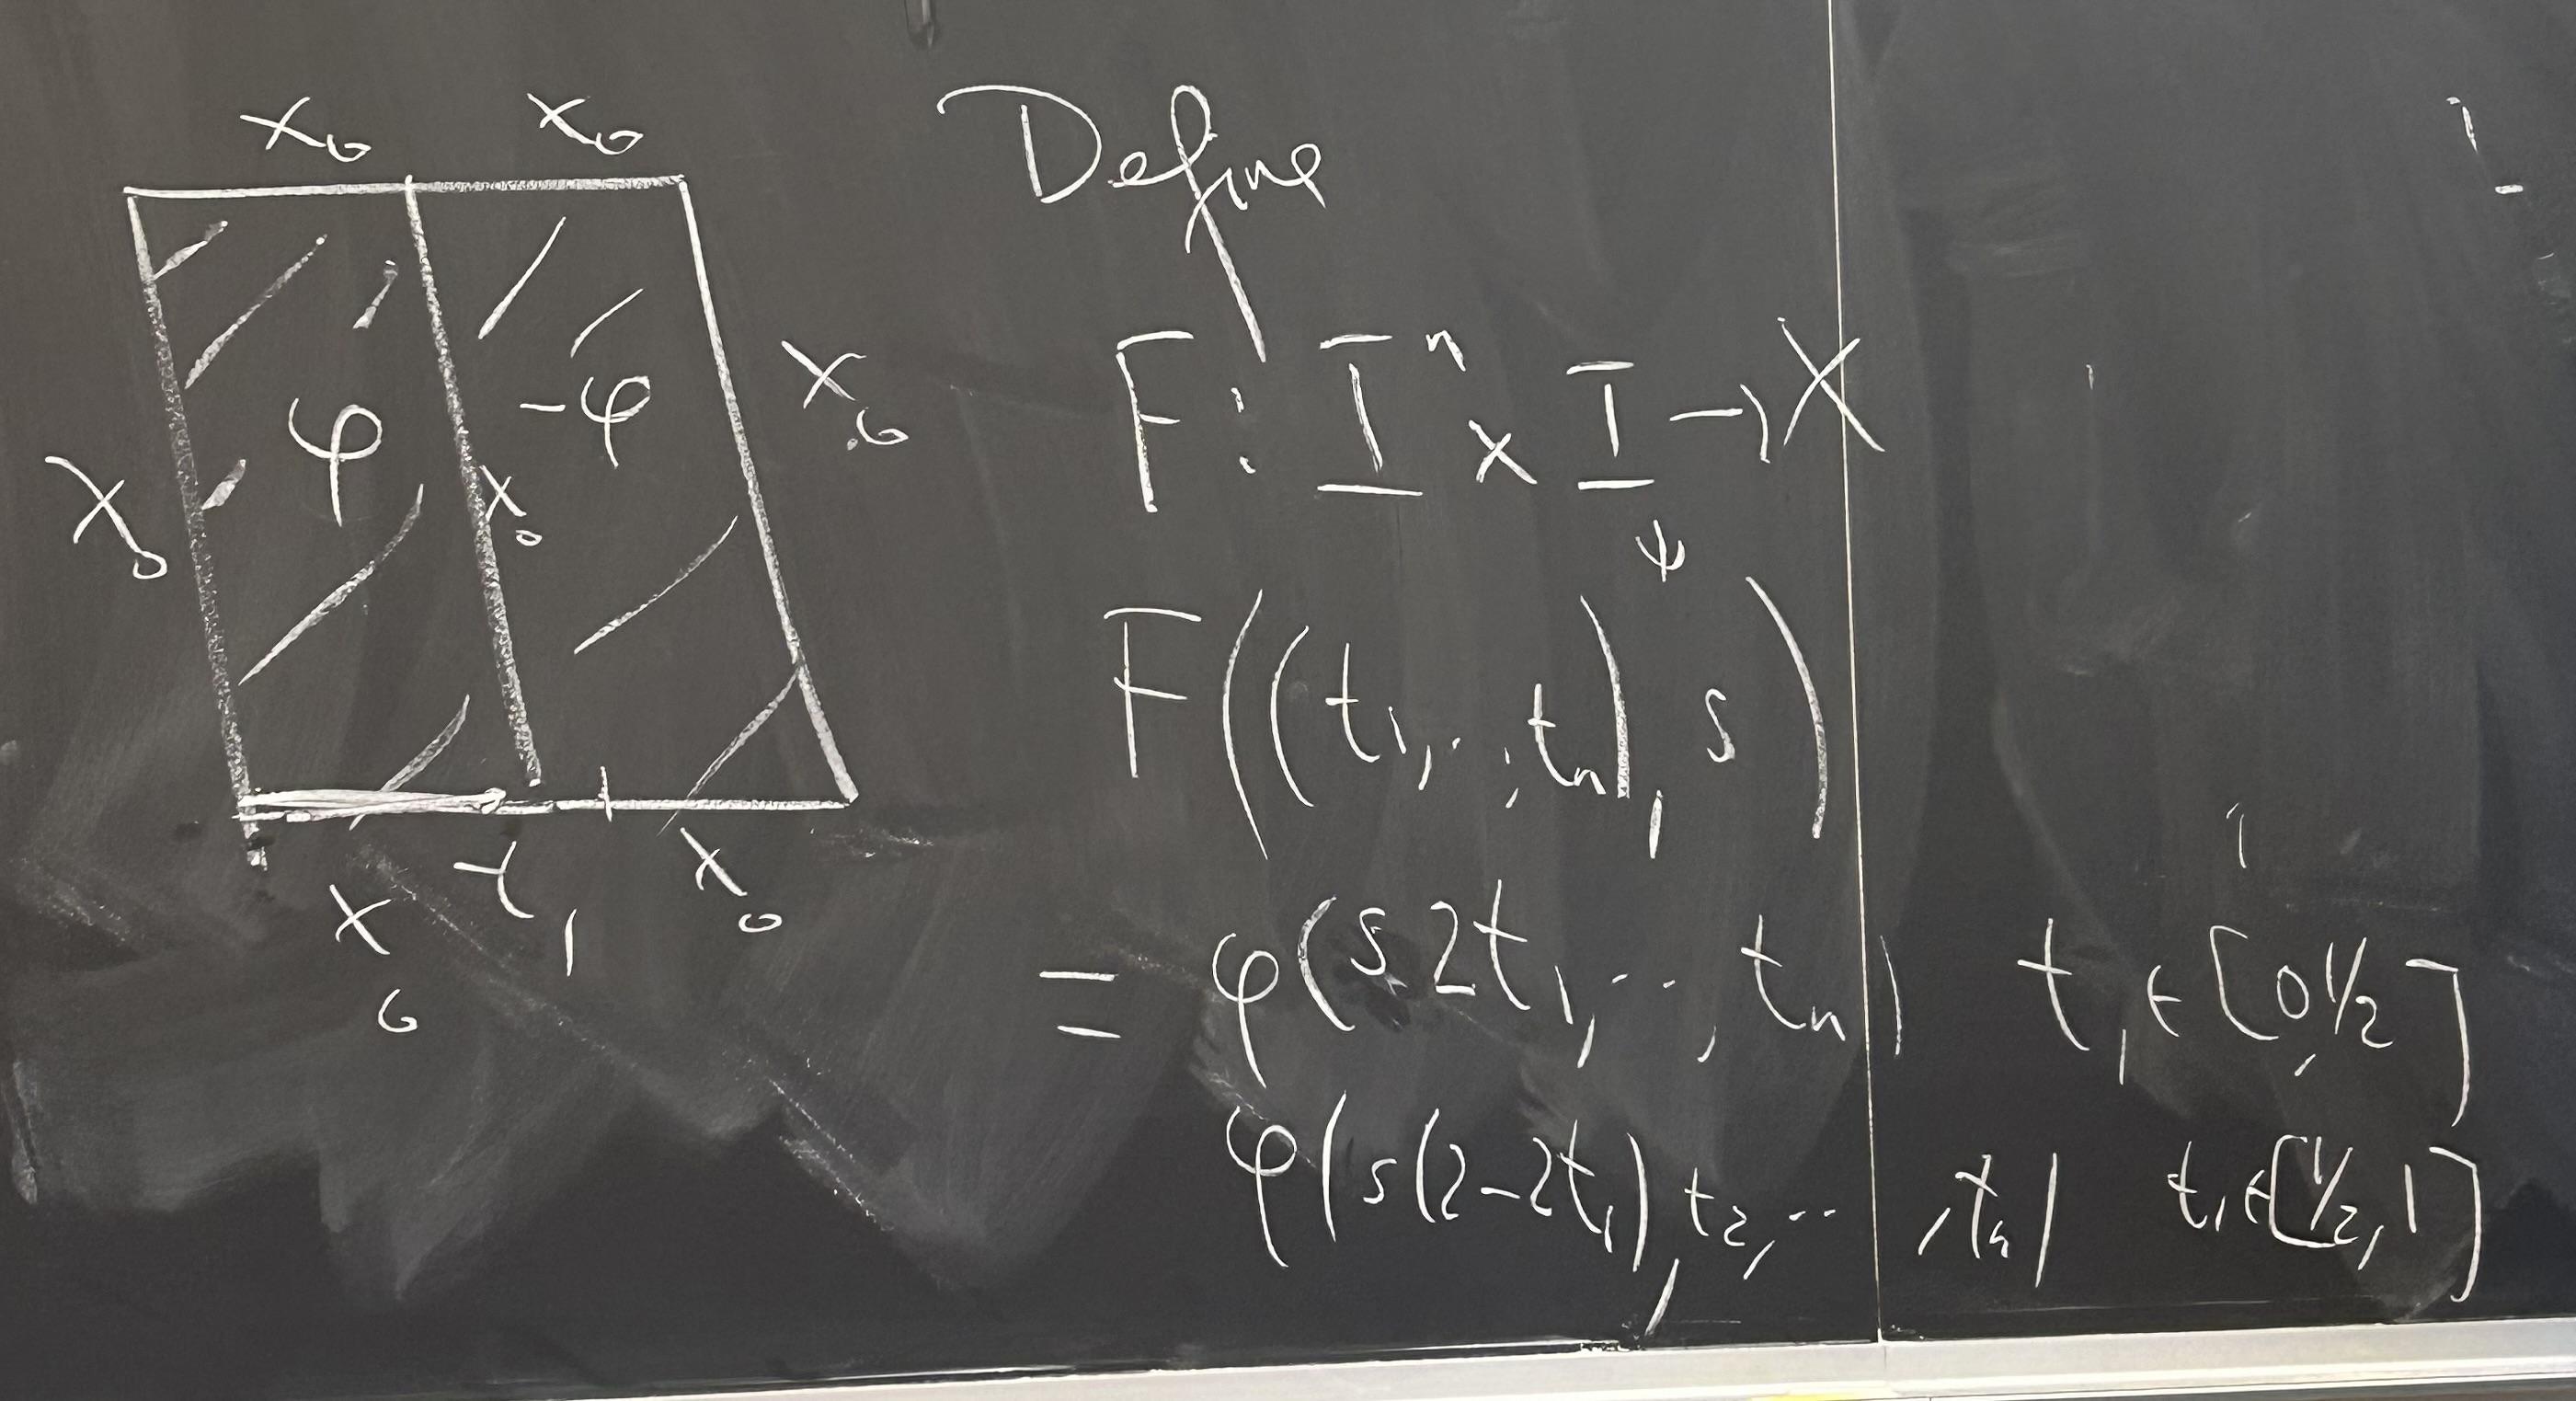
\includegraphics[width=0.6\textwidth]{Figures/pin_associative.jpeg}\]
        \item One can check this is associative in almost the exact same way they would check for $\pi_1$.
        \item For abelian when $n \geq 2$, let us suppose $\varphi, \psi: I^n \to X$ again. Now, here is a pictorial explanation of why they commute for $n \geq 2$,
        \[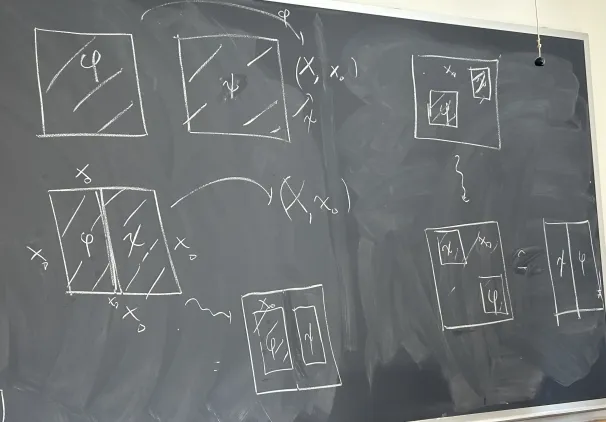
\includegraphics[width=0.6\textwidth]{Figures/pin_abelian.png}\]
    \end{enumerate}
\end{proof}

\begin{definition}
    If $f: (X, x_0) \to (Y, y_0)$ is a map, then $f_*: \pi_n(X, x_0) \to \pi_n(Y, y_0)$ is a group homomophism (taking $[\varphi] \in \pi_n(X, x_0)$ and send it to $[f \circ \varphi] \in \pi_n(Y, y_0)$). In fact, you can even check that $f_* \varphi + f_* \psi = f_*(\varphi + \psi)$ are literally equal as maps.
\end{definition}

\subsection{H-Spaces}

Now we make an observation that
\begin{align*}
    \pi_n(S^n, X) &\cong \pi_n(\Sigma S^{n-1}, X)\\
    &\cong \pi_{n-1}(\Omega X) \tag*{Loop-Suspension Adjunction}
\end{align*}
Recall that $\Omega X = \{\gamma: I \to X\ |\ \gamma(0) = \gamma(1) = x_0\}$. There is a standard map
\[\mu: \Omega X \times \Omega X \to \Omega X\]
given by
\[\mu(\gamma_1, \gamma_2)(t) = \begin{cases}
    \gamma_1(2t), t \in [0, \frac{1}{2}]\\
    \gamma_2(2t-1), t \in [\frac{1}{2}, 1]
\end{cases}.\]
This map $\mu$ descends to a map on $\Omega \wedge \Omega$ since it respects the equivalence relation.

\begin{proposition}
Consider the following diagram
% https://q.uiver.app/#q=WzAsNCxbMCwwLCJcXE9tZWdhIFggXFx3ZWRnZSBcXE9tZWdhIFggXFx3ZWRnZSBcXE9tZWdhIFgiXSxbMCwxLCJcXE9tZWdhIFggXFx3ZWRnZSBcXE9tZWdhIFgiXSxbMSwwLCJcXE9tZWdhIFggXFx3ZWRnZSBcXE9tZWdhIFgiXSxbMSwxLCJcXE9tZWdhIFgiXSxbMCwxLCJcXG11IFxcd2VkZ2UgMV97XFxPbWVnYSBYfSJdLFsxLDMsIlxcbXUiXSxbMiwzLCJcXG11Il0sWzAsMiwiMV97XFxPbWVnYSBYfSBcXHdlZGdlIFxcbXUiLDJdXQ==
\[\begin{tikzcd}
	{\Omega X \wedge \Omega X \wedge \Omega X} & {\Omega X \wedge \Omega X} \\
	{\Omega X \wedge \Omega X} & {\Omega X}
	\arrow["{1_{\Omega X} \wedge \mu}"', from=1-1, to=1-2]
	\arrow["{\mu \wedge 1_{\Omega X}}", from=1-1, to=2-1]
	\arrow["\mu", from=1-2, to=2-2]
	\arrow["\mu", from=2-1, to=2-2]
\end{tikzcd}\]
This map does not usually commute, but they do commute up to homotopy (homotopy commutative). 
\end{proposition}

Let $c_{x_0}: I \to X$ be the constant map, as a coroolary of the proposition, one can check
\[\mu(\gamma, c_{x_0}) \simeq \gamma, \mu(c_{x_0}, \gamma) \simeq \gamma\]
Setting $\gamma^{-1}(t) = \gamma(1-t)$, we also have that
\[\mu(\gamma, \gamma^{-1}) \simeq c_{x_0}.\]

In particular, this means that we have a two-sided identity up to homotopy and we have an inverse up to homotopy.

\begin{definition}
    An $H$-space is a based space $(Y, y_0)$ such that there exists a map $\mu: Y \wedge Y \to Y$ satisfying the hypothesis presented above. This is sometimes also called an $H$-group.
\end{definition}

Our discussion above shows that
\begin{proposition}
    $\Omega X$ is an $H$-group.
\end{proposition}

\begin{theorem}
If $(Y, y_0)$ is an $H$-group, then $[(X, x_0), (Y, y_0)]_*$ may be given a group structure.
\end{theorem}

As examples, this group structure is compatible with the isomorphism
\[\pi_n(X, x_0) \cong \pi_{n-1}(\Omega X, c_{x_0})\]
($\pi_{n-1}(\Omega X, c_{x_0})$ can be given a group structure from $\Omega X$ be a $H$-group, which will be compatible with the homotopy group structure).\\

As another example, suppose $G$ is a topological group, we can define two structures on $\pi_n(G)$, which will turn out to be the same group structure. In fact, you can use the \textbf{Eckmann-Hilton argument} from this to show that $\pi_1(G)$ is abelian.

\begin{remark}
    We defined $\varphi + \psi$ on $I^n$. Here is a picture of how it will look like on $S^n$:
     \[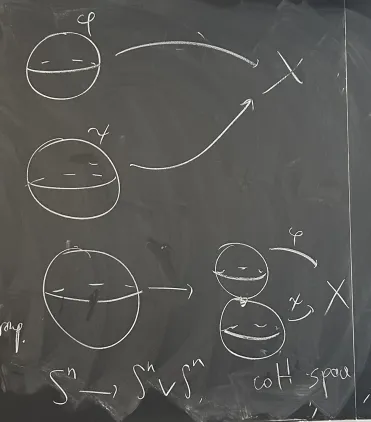
\includegraphics[width=0.5\textwidth]{Figures/coh.png}\]
    This turns $S^n$ into an example of what is called a \textbf{co-H-space}.
\end{remark}

\newpage
\section{Lecture September 10th, 2024}

Last time, we defined the functors of the form
\[\pi_n: T_* \to \begin{cases}
    \text{Pointed Sets}, n = 0\\
    \text{Groups}, n = 1\\
    \text{Abelian Groups}, n \geq 2
\end{cases}.\]
There is a sequence of forgetful functors from Abelian Groups to Groups, and then Groups to Pointed Sets.\\

From here, we defined
\[\pi_n(X, x_0) = [(S^n, s_0), (X_, x_0)]_* \cong [(I^n, \partial I^n), (X, x_0)]_* \cong \pi_{n-1}(\Omega X, *).\]

\subsection{Path Invariance of $\pi_n$}

\begin{question}
    How does $\pi_n(X, x_0)$ depend on $x_0$?
\end{question}

The answer turns out to be relatively simple - 

\begin{proposition}
Suppose $x_0, x_1$ are in the same path component of $X$, $\pi_n(X, x_0)$ is isomorphic to $\pi_n(X, x_1)$. Specifically, there exists $\gamma: I \to X$ such that $\gamma(0) = x_0, \gamma(1) = x_1$ that induces an isomorphism
\[h_{\gamma}: \pi_n(X, x_0) \to \pi_n(X, x_1). \]
\end{proposition}

\begin{proof}
    Suppose $\varphi: (I^n, \partial I^n) \to (X, x_0)$, 
    \[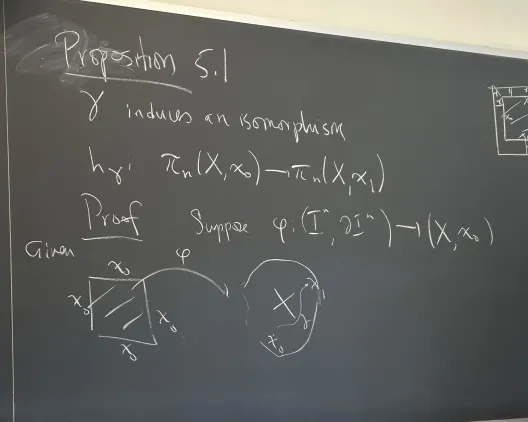
\includegraphics[width=0.5\linewidth]{Figures/varphi.png}\]
    We could modify $\varphi$ to a function $h_{\gamma}(\varphi)$ becomes the follow:
    \[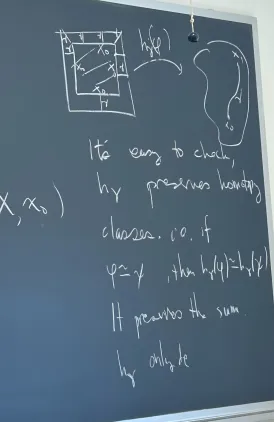
\includegraphics[width=0.3\linewidth]{Figures/modified_varphi.png}\]
    Here we do $\varphi$ on the inside, and once we reach boundary, we connect by the path $\gamma$. It is easy to check that $h_{\gamma}$ preserves homotopy classes, ie.
    \[\varphi \simeq \psi \implies h_\gamma(\varphi) \simeq h_\gamma(\psi),\]
    and the $h_{\gamma}$ preserves the sum. We can check that $h^{-1}_{\gamma} = h_{\gamma^{-1}}$, where $\gamma^{-1}: I \to X$ is defined by $\gamma^{-1}(t) = \gamma(1 - t)$.\\

    Thus, this means that $h_{\gamma}$ is an isomorphism.
\end{proof}

\begin{remark}
    Finally, we note the function $h_{\gamma}$ only depends on the homotopy class of $\gamma$ rel $\partial I$. If $x_0 = x_1$, $\gamma$ a loop of $x_0$, the proof outlined above defined an action of $\pi_1(X, x_0)$ on $\pi_n(X, x_0)$.
\end{remark}

\begin{proposition}
    If $(X, x_0)$ is based contractible in $T^*$, then $\pi_n(X, x_0) = 0$ for all $n$.
\end{proposition}

\begin{proof}
    Exercise.
\end{proof}

\subsection{Covering Space Isomorphism of $\pi_n$}
\begin{proposition}
    Suppose $p: (Y, y_0) \to (X, x_0)$ is a covering space, this induces a map $p_*: \pi_n(Y, y_0) \to \pi_n(X, x_0)$. This is an isomorphism for $n \geq 2$.
\end{proposition}

\begin{proof}
    The key property of a covering space is that it has the homotopy lifting property. For \textbf{surjectivity}, suppose $\varphi: (S^n, s_0) \to (X, x_0)$, since $S^n$ is simply connected for $n \geq 2$ (so the map $\varphi$ is $0$ on the level of $\pi_1$), thus we have a lift
    % https://q.uiver.app/#q=WzAsMyxbMCwxLCIoU15uLCBzXzApIl0sWzEsMSwiKFgsIHhfMCkiXSxbMSwwLCIoWSwgeV8wKSJdLFswLDFdLFsyLDEsInAiLDJdLFswLDIsIiIsMix7InN0eWxlIjp7ImJvZHkiOnsibmFtZSI6ImRhc2hlZCJ9fX1dXQ==
\[\begin{tikzcd}
	& {(Y, y_0)} \\
	{(S^n, s_0)} & {(X, x_0)}
	\arrow["p"', from=1-2, to=2-2]
	\arrow[dashed, from=2-1, to=1-2]
	\arrow[from=2-1, to=2-2]
\end{tikzcd}.\] (More generally, $\varphi_*(\pi_1(S^n, s_0)) \subseteq p_*(\pi_1(Y, y_0))$ is enough to give a lift). Hence, $\varphi$ lifts to $\Tilde{\varphi}$ such that $\rho \circ \Tilde{\varphi} = \varphi$.\\

For \textbf{injectivity}, if $\varphi: (S^n, s_0) \to (Y, y_0)$ is in the kernel of $p_*$, then we want to show that $[\varphi] = 0$. Since $p_*(\varphi) = 0$, there exists a homotopy $H: S^n \times I \to X$ such that
\[H(s, 0) = p \circ \varphi \text{ and } H(s, 1) = c_{x_0}.\]
(Recall $c_{x_0}$ is the constant map with value $x_0$). This is exactly where we use the homotopy lifting property. By the covering homotopy property, there exists an unique $\Tilde{H}: S^n \times I \to (Y, y_0)$ lifting $H$, such that
\[\Tilde{H}(s, 0) = \varphi(s), \Tilde{H}(s, 1) = c_{y_0}.\]
\end{proof}

\begin{question}
    Does this proof work with any simply connected co-H-space? (Ex. The suspension of any space is a co-H-space.)
\end{question}

\begin{corollary}
    If $X$ is any space such that its \textbf{universal cover} $\Tilde{X}$ is contractible, then
    \[\pi_n(X, x_0) = 0, n \geq 2.\]
\end{corollary}

\begin{definition}
    If $X$ is a space such that $\Tilde{X}$ is contractible (this is equivalent to $\pi_n(X, x_0) = 0$ for $n \geq 2$ on CW complexes), $X$ is called \textbf{aspherical}. We sometimes write $X =  K(\pi, 1)$.
\end{definition}

\begin{example}
    Here are some examples of aspherical spaces:
    \begin{enumerate}
        \item $\Rbb P^{\infty}$
        \item $S^1$
        \item $S^1 \times S^1$
    \end{enumerate}
    In general, if $\Gamma$ is a group acting freely and properly discontinuously on $Y$, which is contractible, then $Y \to Y/\Gamma$ is contractible and $Y/\Gamma$ is aspherical. For example
    \begin{enumerate}
        \item $S^1 \times S^1 = \Rbb^2/\Zbb^2$.
        \item If we take $H$ to be the Heisenberg group
        \[H = \{\begin{pmatrix}
            1 & a & c\\
            0 & 1 & b\\
            0 & 0 & 1
        \end{pmatrix}\ |\ a, b, c \in \Rbb\}\]
        We take
        \[\Gamma =  \{\begin{pmatrix}
            1 & a & c\\
            0 & 1 & b\\
            0 & 0 & 1
        \end{pmatrix}\ |\ a, b, c \in \Zbb\}\]
        Then $H/\Gamma$ is aspherical.
        \item If $G$ is a connected Lie group (eg. $SL_n(\Rbb)$), there exists a maximal compact subgroup $K$ such that $G/K$ is homeomorphic to $\Rbb^n$ for some $n$.
        \item Furthermore, if $\Gamma \subseteq G$ is discrete and torsion free, the double coset $\Gamma \backslash G / K$ is aspherical.
        \item On $G = SL_n(\Rbb)$, $K = SO(n)$.
        \item If $n = 2$, $\operatorname{SL}_2(\Rbb)/SO(2) \cong \mathbb{H}^2$ is the upper half plane. If $\Gamma \subseteq \operatorname{SL}_2(\Rbb)$, then $\Gamma \backslash \mathbb{H}^2$ is a surface.
    \end{enumerate}
\end{example}

\begin{conjecture}[Borel Conjecture]
    If $X, Y$ are aspherical manifolds and $\pi_1(X) \cong \pi_1(Y)$, then $X$ is homeomorphic to $Y$.
\end{conjecture}

\subsection{Cofibration and Homotopy Extension Property}
In the homework, you are asked to deal with an example of bad space $(X, A)$ where $A$ is contractible, but $q: X \to X/A$ is not a homotopy equivalence! We want to consider spaces where this cannot happen.

\begin{definition}[Homotopy Extension Property (HEP)]
    Let $i: A \to X$ be a map. Suppose $f: X \to Y$ is a map in $T$, and we have a homotopy $H: A \times I \to Y$ from $f \circ i$ to some other map $g$. An extension of $H$ is a map $\undertilde{H}: X \times I \to Y$ such that
    \begin{itemize}
        \item $\undertilde{H}|_{A \times I} = H$.
        \item $\undertilde{H}(x, 0)= f(x)$.
    \end{itemize}
    Pictorially, 
    % https://q.uiver.app/#q=WzAsNSxbMCwwLCJBIFxcdGltZXMgXFx7MFxcfSJdLFsxLDAsIlggXFx0aW1lcyBcXHswXFx9Il0sWzAsMSwiQSBcXHRpbWVzIEkiXSxbMSwxLCJYIFxcdGltZXMgSSJdLFsyLDIsIlxcYnVsbGV0Il0sWzAsMSwiaSJdLFswLDIsIiIsMix7InN0eWxlIjp7InRhaWwiOnsibmFtZSI6Imhvb2siLCJzaWRlIjoiYm90dG9tIn19fV0sWzIsMywiaSBcXHRpbWVzIDFfSSIsMl0sWzEsMywiIiwwLHsic3R5bGUiOnsidGFpbCI6eyJuYW1lIjoiaG9vayIsInNpZGUiOiJ0b3AifX19XSxbMSw0XSxbMiw0LCJIIiwyXSxbMyw0LCJcXHVuZGVydGlsZGV7SH0iLDEseyJzdHlsZSI6eyJib2R5Ijp7Im5hbWUiOiJkYXNoZWQifX19XV0=
\[\begin{tikzcd}
	{A \times \{0\}} & {X \times \{0\}} \\
	{A \times I} & {X \times I} \\
	&& \bullet
	\arrow["i", from=1-1, to=1-2]
	\arrow[hook', from=1-1, to=2-1]
	\arrow[hook, from=1-2, to=2-2]
	\arrow["f", from=1-2, to=3-3]
	\arrow["{i \times 1_I}"', from=2-1, to=2-2]
	\arrow["H"', from=2-1, to=3-3]
	\arrow["{\undertilde{H}}"{description}, dashed, from=2-2, to=3-3]
\end{tikzcd}\]
We say that $i: A \to X$ has the homotopy extension property with respect to a fixed $Y$ if for any extension problems involving (unfixed) $(H, f)$ like the diagram above admits a $\undertilde{H}$.
\end{definition}

\begin{definition}
    $i: A \to X$ is a \textbf{cofibration} (Hurewicz) if it has the HEP with respect to any $Y \in T$.
\end{definition}

\textbf{FACT: } Any cofibration is a closed inclusion.

\begin{definition}
    A subset $B \subseteq X$ is a retract if there exists $r: X \to B$ such that $r \circ i = 1_B$ (here $i: B \to X$ is the inclusion map).
\end{definition}

\begin{lemma}
    $i: A \to X$ is a cofibration if and only if $A \times I \cup X \times \{0\} \subseteq X \times I$ is a retract.
\end{lemma}

\begin{proof}
    Suppose $i: A \to X$ is a cofibration, we consider the following extension problem
    % https://q.uiver.app/#q=WzAsNSxbMCwwLCJBIFxcdGltZXMgXFx7MFxcfSJdLFswLDEsIkEgXFx0aW1lcyBJIl0sWzEsMCwiWCBcXHRpbWVzIFxcezBcXH0iXSxbMSwxLCJYIFxcdGltZXMgSSJdLFsyLDIsIkEgXFx0aW1lcyBJIFxcY3VwIFggXFx0aW1lcyBcXHswXFx9Il0sWzAsMV0sWzIsM10sWzEsM10sWzAsMl0sWzIsNCwiaW5jbHVzaW9uIl0sWzEsNCwiaW5jbHVzaW9uIiwyXSxbMyw0LCJyIiwwLHsic3R5bGUiOnsiYm9keSI6eyJuYW1lIjoiZGFzaGVkIn19fV1d
\[\begin{tikzcd}
	{A \times \{0\}} & {X \times \{0\}} \\
	{A \times I} & {X \times I} \\
	&& {A \times I \cup X \times \{0\}}
	\arrow[from=1-1, to=1-2]
	\arrow[from=1-1, to=2-1]
	\arrow[from=1-2, to=2-2]
	\arrow["inclusion", from=1-2, to=3-3]
	\arrow[from=2-1, to=2-2]
	\arrow["inclusion"', from=2-1, to=3-3]
	\arrow["r", dashed, from=2-2, to=3-3]
\end{tikzcd}\]
Since $i: A \to X$ is a cofibration, we solve the extension problem with the map $r$. One can check that this is the retraction we desire (just by commutativity od the diagram).\\

Conversely, suppose we have a retract $r: X \times I \to A \times I \cup X \times \{0\}$ and consider the extension problem 
% https://q.uiver.app/#q=WzAsNixbMCwwLCJBIFxcdGltZXMgXFx7MFxcfSJdLFsxLDAsIlggXFx0aW1lcyBcXHswXFx9Il0sWzAsMSwiQSBcXHRpbWVzIEkiXSxbMSwxLCJYIFxcdGltZXMgSSJdLFsyLDIsIkEgXFx0aW1lcyBJIFxcY3VwIFggXFx0aW1lcyBcXHswXFx9Il0sWzIsMywiWSJdLFswLDJdLFswLDFdLFsyLDNdLFsxLDNdLFszLDQsInIiLDJdLFsyLDUsIkgiLDJdLFsxLDUsImYiLDAseyJvZmZzZXQiOi01fV0sWzQsNSwiSCBcXGN1cCBmIiwwLHsib2Zmc2V0IjotNX1dXQ==
\[\begin{tikzcd}
	{A \times \{0\}} & {X \times \{0\}} \\
	{A \times I} & {X \times I} \\
	&& {A \times I \cup X \times \{0\}} \\
	&& Y
	\arrow[from=1-1, to=1-2]
	\arrow[from=1-1, to=2-1]
	\arrow[from=1-2, to=2-2]
	\arrow["f", shift left=5, from=1-2, to=4-3]
	\arrow[from=2-1, to=2-2]
	\arrow["H"', from=2-1, to=4-3]
	\arrow["r"', from=2-2, to=3-3]
	\arrow["{H \cup f}", shift left=5, from=3-3, to=4-3]
\end{tikzcd}\]
Here we can check that $(H \cup f) \circ r = \undertilde{H}$ is the esired solution to the extension problem.
\end{proof}

\begin{example}
    Here are some examples of cofibrations.
    \begin{enumerate}
        \item The inclusion map $A \to X = A \times I$ given by $a \mapsto (a, 0)$ is a cofibration. To do this, we need to show there is a retraction with respect to $A \times I \cup X \times \{0\} \to X \times I$, which is just showing that $A \times \{0\} \times I \cup A \times I \times \{0\} \to A \times I \times I$ admits a retraction.\\

        To show this has a retraction, we fix the first component and squich the square $I \times I$ down to its two sides $\{0\} \times I \cup I \times \{0\}$.

        \item Consider the inclusion map $S^{n-1} \to D^n$. In this case, $S^{n-1} \times I \cup D^n times \{0\} \subseteq D^n \times I$. Pictorically, we can see that there is not only a retract (but a deformation retract):
    \[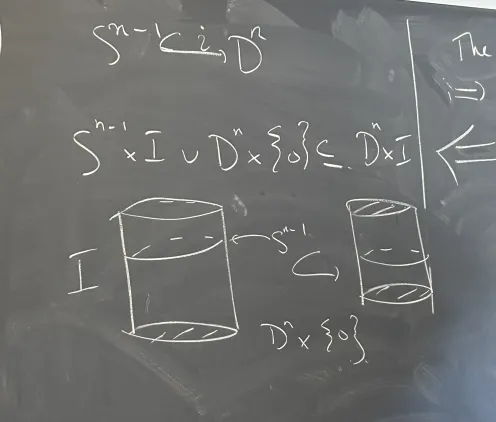
\includegraphics[width=0.5\linewidth]{Figures/can.png}\]
        by pushing down the solid core in the right hand side until it becomes the left hand side.
    \end{enumerate}
\end{example}

\begin{definition}
    Suppose $f: X \to Y$ is a map in $T$, we define the mapping cylinder $\operatorname{Cyl}(f)$ as the following:
        \[X \times I \sqcup Y/\sim, (x, 1) \sim f(x)\]
        There is a map $i: X \to \operatorname{Cyl}(f)$ that sends $x \mapsto (x, 0)$, and a map $p: \operatorname{Cyl}(f) \to Y$ with $p(x, t) = f(x)$ and $p(y) = y$. \textbf{Note:} If $f: X \to pt$ is the constant map, then $\operatorname{Cyl}(f) = X \times I \cup pt/\sim$ is just the unreduced cone $C(X)$.
\end{definition}

\begin{proposition}
We can factor our map $f: X \to Y$ as the following
    % https://q.uiver.app/#q=WzAsMyxbMCwwLCJYIl0sWzEsMCwiXFxvcGVyYXRvcm5hbWV7Q3lsfShmKSJdLFsyLDAsIlkiXSxbMCwxLCJpIl0sWzEsMiwicCJdLFswLDIsImYiLDAseyJvZmZzZXQiOi01fV1d
\[\begin{tikzcd}
	X & {\operatorname{Cyl}(f)} & Y
	\arrow["i", from=1-1, to=1-2]
	\arrow["f", shift left=5, from=1-1, to=1-3]
	\arrow["p", from=1-2, to=1-3]
\end{tikzcd}\]
where $i$ is a cofibration and $p$ is a homotopy equivalence.
\end{proposition}

We know that a map $X \times I \to Y$ is equivalent to $X \to \underline{T}(I, Y)$ (adjoint property). Using this adjoint property, we can reinterpret the solvability of
% https://q.uiver.app/#q=WzAsNSxbMCwwLCJBIl0sWzEsMCwiWCJdLFswLDEsIkEgXFx0aW1lcyBJIl0sWzEsMSwiWCBcXHRpbWVzIEkiXSxbMiwyLCJZIl0sWzAsMSwiaSJdLFsyLDMsImkiXSxbMCwyXSxbMSwzXSxbMSw0XSxbMiw0XV0=
\[\begin{tikzcd}
	A & X \\
	{A \times I} & {X \times I} \\
	&& Y
	\arrow["i", from=1-1, to=1-2]
	\arrow[from=1-1, to=2-1]
	\arrow[from=1-2, to=2-2]
	\arrow[from=1-2, to=3-3]
	\arrow["i", from=2-1, to=2-2]
	\arrow[from=2-1, to=3-3]
    \arrow["\Tilde{H}", dotted, from=2-2, to=3-3]
\end{tikzcd}\]
into having a lift for the following diagram
% https://q.uiver.app/#q=WzAsNCxbMCwwLCJBIl0sWzAsMSwiWCJdLFsxLDAsIlxcdW5kZXJsaW5le1R9KEksWSkiXSxbMSwxLCJZIl0sWzAsMSwiaSIsMl0sWzAsMiwiXnQgSCJdLFsyLDMsInAiXSxbMSwzLCJmIiwyXSxbMSwyLCJedCBcXFRpbGRle0h9IiwxLHsic3R5bGUiOnsiYm9keSI6eyJuYW1lIjoiZG90dGVkIn19fV1d
\[\begin{tikzcd}
	A & {\underline{T}(I,Y)} \\
	X & Y
	\arrow["{^t H}", from=1-1, to=1-2]
	\arrow["i"', from=1-1, to=2-1]
	\arrow["p", from=1-2, to=2-2]
	\arrow["{^t \Tilde{H}}"{description}, dotted, from=2-1, to=1-2]
	\arrow["f"', from=2-1, to=2-2]
\end{tikzcd}\]
Here $p$ sends $\varphi: I \to Y$ to $\varphi(0)$. In other words, $i$ is a cofibration if and only if this diagram above is always solvable.

\begin{remark}
    $\underline{T}(I, Y)$ is homotopy equivalent to $Y$ (you start out with any path and go back to the start).
\end{remark}

\begin{example}
    If $A \subseteq X$ is a sub-CW-complex, then the inclusion $A \to X$ is a cofibration.
\end{example}



\newpage
\section{Lecture September 12th 2024}

\subsection{Homotopy Version of Tubular Neighborhood}
Recall last time we proved.
\begin{proposition}
    The inclusion map $i: A \to X$ satisfies the HEP relative to any space in $T_*$ if and only if $A \times I \cup X \times \{0\} \to X \times I$ has a retraction.
\end{proposition}

This is a homotopy version of a tubular neighborhood.

\begin{proposition}
 $i: A \to X$ is a cofibration if and only if there exists closed neighborhood $N \subseteq X$, and $A \subseteq N$, $B \subseteq N$, such that $N \setminus B$ is an open neighborhood of $A$ in $X$, and there is a map $r: B \to A$ with a homeomorphic $h: \operatorname{Cyl}(r) \to N$ such that $h|_{A \cup B} = id$.
\end{proposition}

\begin{remark}
    $r: B \to A$ is not necessarily the retraction. We just used the letter for some reason.
\end{remark}

Here is a picture to have in mind:
\[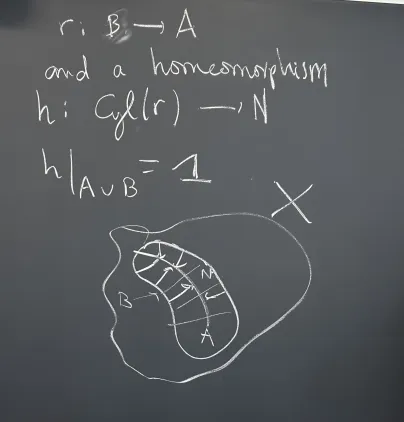
\includegraphics[width=0.5\textwidth]{Figures/tubular_neighborhood.png}\]
In the picture, $N$ is the ``tubular neighborhood" and $B$ is the ``boundary".

\begin{example}
    If $M$ is a differentiable manifold and $A \subseteq M$ is a closed submanifold, then ther exists a tubular neighborhood $N$ containing $A$ such that $N$ is diffeomorphic to a neighborhood of the $0$-section of a normal bundle of $A$ in $M$.
\end{example}

Last time, we saw that for any continuous map $f: X \to Y$, we can factor it as
% https://q.uiver.app/#q=WzAsMyxbMCwwLCJYIl0sWzIsMCwiWSJdLFsxLDEsIlxcb3BlcmF0b3JuYW1le0N5bH0oZikiXSxbMCwyLCJpIl0sWzIsMSwicCwgXFxzaW1lcSJdLFswLDEsImYiXV0=
\[\begin{tikzcd}
	X && Y \\
	& {\operatorname{Cyl}(f)}
	\arrow["f", from=1-1, to=1-3]
	\arrow["i", from=1-1, to=2-2]
	\arrow["{p, \simeq}", from=2-2, to=1-3]
\end{tikzcd}\]
where $i$ is a cofibration and $p$ is a homotopy equivalence.

\begin{remark}
    You should think of cofibrations as the homotopic version of ``projective objects".
\end{remark}

\begin{definition}
    A space $X \in T_*$ is \textbf{cofibrant} if the canonical map from basepoint $* \to X$ is a cofibration.
\end{definition}

\subsection{Fibrations}

\begin{question}
    What is the analogy for an injective module?
\end{question}

\begin{definition}
    A map $p: Y \to X$ has the \textbf{homotopy lifting property} (HLP) relative to $A$ if given a lifting problem, it has a solution for all $H, f$ given
    % https://q.uiver.app/#q=WzAsNCxbMCwwLCJBIl0sWzAsMSwiQSBcXHRpbWVzIEkiXSxbMSwwLCJZIl0sWzEsMSwiWCJdLFswLDEsImlfMCIsMix7InN0eWxlIjp7InRhaWwiOnsibmFtZSI6Imhvb2siLCJzaWRlIjoidG9wIn19fV0sWzAsMiwiZiJdLFsyLDMsInAiXSxbMSwzLCJIIiwyXSxbMSwyLCJcXFRpbGRle0h9IiwxLHsic3R5bGUiOnsiYm9keSI6eyJuYW1lIjoiZGFzaGVkIn19fV1d
\[\begin{tikzcd}
	A & Y \\
	{A \times I} & X
	\arrow["f", from=1-1, to=1-2]
	\arrow["{i_0}"', from=1-1, to=2-1]
	\arrow["p", from=1-2, to=2-2]
	\arrow["{\Tilde{H}}"{description}, dashed, from=2-1, to=1-2]
	\arrow["H"', from=2-1, to=2-2]
\end{tikzcd}\]
Here $i_0: A \to A \times I$ is given by $a \mapsto (a, 0)$. Note $A$ is not necessarily a subspace of $X$. 
\end{definition}

\begin{definition}
    We say $p: Y \to X$ is a \textbf{fibration} if it has the HLP relative to all spaces $Z \in T$.
\end{definition}

Just like how cofibrations have an alternative characterization using the adjoint correspondence between a map $X \times I \to Y$ with a map $X \to \underline{T}(I, Y)$, we also have a equivalent characterization of fibration. The fibration problem is actually equivalent to admitting a solution to the following diagram give $f: A \to Y$ and $^t H: A \to \underline{T}(I, X)$:
% https://q.uiver.app/#q=WzAsNSxbMCwwLCJBIl0sWzEsMSwiXFx1bmRlcmxpbmV7VH0oSSwgWSkiXSxbMiwxLCJcXHVuZGVybGluZXtUfShJLCBYKSJdLFsyLDIsIlgiXSxbMSwyLCJZIl0sWzAsMSwiXFxleGlzdHMgXFxUaWxkZXtIfSIsMSx7InN0eWxlIjp7ImJvZHkiOnsibmFtZSI6ImRhc2hlZCJ9fX1dLFsxLDIsInBfKiwgXFxnYW1tYSBcXG1hcHN0byBwIFxcY2lyYyBcXGdhbW1hIl0sWzIsMywiZV8wIl0sWzEsNCwiZV8wIl0sWzQsMywicCIsMl0sWzAsMiwiSCIsMCx7Im9mZnNldCI6LTV9XSxbMCw0LCJmIiwyLHsib2Zmc2V0Ijo1fV1d
\[\begin{tikzcd}
	A \\
	& {\underline{T}(I, Y)} & {\underline{T}(I, X)} \\
	& Y & X
	\arrow["{\exists ^t \Tilde{H}}"{description}, dashed, from=1-1, to=2-2]
	\arrow["^t H", shift left=5, from=1-1, to=2-3]
	\arrow["f"', shift right=5, from=1-1, to=3-2]
	\arrow["{p_*, \gamma \mapsto p \circ \gamma}", from=2-2, to=2-3]
	\arrow["{e_0}", from=2-2, to=3-2]
	\arrow["{e_0}", from=2-3, to=3-3]
	\arrow["p"', from=3-2, to=3-3]
\end{tikzcd} (\dagger)\]

\begin{example}
    Consider the standard projection map $p: X \times I \to X$. This is a fibration. Indeed, consider the following diagram
    % https://q.uiver.app/#q=WzAsNCxbMCwwLCJaIl0sWzAsMSwiWiBcXHRpbWVzIEkiXSxbMSwwLCJYIFxcdGltZXMgSSJdLFsxLDEsIlgiXSxbMCwxLCJpXzAiLDJdLFsxLDMsIkgiLDJdLFswLDIsImYiXSxbMiwzLCJwIl1d
\[\begin{tikzcd}
	Z & {X \times I} \\
	{Z \times I} & X
	\arrow["f", from=1-1, to=1-2]
	\arrow["{i_0}"', from=1-1, to=2-1]
	\arrow["p", from=1-2, to=2-2]
	\arrow["H"', from=2-1, to=2-2]
\end{tikzcd}\]
Write $f(z) = (f_1(z), f_2(z))$ where $f_1: Z \to X$ and $f_2: Z \to I$. From here, we define the lift to be
\[\Tilde{H}(z, t) = (H(z, t), f_2(z)).\]
Note the proof is completely independent of $I$, we could have chosen any projection $p: X \times Y \to X$.
\end{example}

The following is a very deep theorem that we probably will not prove.
\begin{theorem}
    If $p: Y \to X$ is locally a fibration just between spaces in $T$, then it is a fibration. By a local fibration, we mean for all $x \in X$, there exists a neighborhood $x \in U$ and a neighborhood such that $\rho^{-1}(U) \to U$ is a fibration.
\end{theorem}

\begin{definition}
    $p: Y \to X$ is a fiber bundle if there exists a space $F$ such that for all $x \in X$, there exists a neighborhood $U$ containing $x$, such that the following diagram commutes
    % https://q.uiver.app/#q=WzAsMyxbMCwwLCJcXHJob157LTF9KFUpIl0sWzIsMCwiVSBcXHRpbWVzIEYiXSxbMSwxLCJVIl0sWzAsMiwicCJdLFswLDEsIlxcY29uZyJdLFsxLDIsIlxccGkiLDJdXQ==
\[\begin{tikzcd}
	{\rho^{-1}(U)} && {U \times F} \\
	& U
	\arrow["\cong", from=1-1, to=1-3]
	\arrow["p", from=1-1, to=2-2]
	\arrow["\pi"', from=1-3, to=2-2]
\end{tikzcd}\]
and the horizontal arrow is a homeomorphism. In this case, $F$ is called the \textbf{fiber} and we can write $F = \rho^{-1}(x)$ for any $x \in X$.
\end{definition}

\begin{corollary}
    Fiber bundle projections $p: Y \to X$ are fibrations.
\end{corollary}

More generally, if $p: Y \to X$ is a fibration, then $p^{-1}(x)$ is called the \textbf{fiber}. The reason this definition makes sense is the following.

\begin{proposition}
    If $x, y$ are in the same path component of $X$ in a fibration $p: Y \to X$, then $p^{-1}(x)$ is homotopy equivalent to $p^{-1}(y)$.
\end{proposition}

\begin{proof}[Added After Class Is Over]
   We are given that $p: Y \to X$ is a fibration. This means that for any map $f: A \to Y$ and homotopy $H: A \times I \to X$ from $p \circ f$ to some other map, the following diagram commutes and admits an extension
    % https://q.uiver.app/#q=WzAsNCxbMCwwLCJBIl0sWzEsMCwiWSJdLFswLDEsIkEgXFx0aW1lcyBJIl0sWzEsMSwiWCJdLFswLDEsImYiXSxbMCwyLCJpXzAiLDJdLFsxLDMsInAiXSxbMiwzLCJIIiwyXSxbMiwxLCJcXFRpbGRle0h9IiwxLHsic3R5bGUiOnsiYm9keSI6eyJuYW1lIjoiZGFzaGVkIn19fV1d
\[\begin{tikzcd}
	A & Y \\
	{A \times I} & X
	\arrow["f", from=1-1, to=1-2]
	\arrow["{i_0}"', from=1-1, to=2-1]
	\arrow["p", from=1-2, to=2-2]
	\arrow["{\Tilde{H}_\gamma}"{description}, dashed, from=2-1, to=1-2]
	\arrow["H_\gamma"', from=2-1, to=2-2]
\end{tikzcd}. \quad (\dagger)\] 
Let $\gamma: [0, 1] \to X$ be a path from $x$ to $y$ in $X$. Consider the inclusion map $f: A = p^{-1}(x) \to Y$ given by and a map $H_\gamma: A \times I \to X$ constructed as follows:
\begin{enumerate}
    \item $H_\gamma(a, t) = \gamma(t)$.
    \item Note that $H_\gamma(a, t)|_{A \times \{0\}}$ is constant onto $x \in X$. On the other hand, $p(p^{-1}(x)) = x$. Thus, the diagram $p \circ f= H_\gamma \circ i_0$.
\end{enumerate}
From the fibration property, we admit a map $\Tilde{H}_\gamma: A \times I \to Y$ lifting $H_\gamma$. Now we observe what this $\Tilde{H}_\gamma$ does:
\begin{enumerate}
    \item For all $a \in A = f^{-1}(x)$, $\Tilde{H}_\gamma(a, 0) = f(a) = a$. In other words, $\Tilde{H}_\gamma|_{A \times \{0\}}$ is the identity on $f^{-1}(x)$.
    \item For all $a \in A = f^{-1}(x)$, $p \circ \Tilde{H}_\gamma(a, 1) = H_\gamma(a, 1) = \gamma(1) = y$. Hence, $\Tilde{H}_\gamma(a, 1) \in p^{-1}(y)$.
    \item From here, we define $f_{\gamma}: p^{-1}(x) \to p^{-1}(y)$ as the map $\Tilde{H}_\gamma(a, 1)$.
\end{enumerate}
We remark that the lift given by the HLP need not be unique, so there may be different choices for $f_{\gamma}$. However, they will all be homotopic to each other because they are given by their respective $\Tilde{H}(a, t)$ that goes back to the same map on $t = 0$. So we do have a well-defined $f_{\gamma}$ up to homotopy.\\

Similarly, let $\gamma^{-1}$ be the inverse path of $\gamma$ and $c_x, c_y$ be the constant path at $x,y$, we can define $(\Tilde{H}_{\gamma^{-1}}, f_{\gamma^{-1}})$, $(\Tilde{H}_{c_x}, f_{c_x})$, and $(\Tilde{H}_{c_y}, f_{c_y})$. We also note that by our construction $f_{c_x}$ and $f_{c_y}$ are actually homotopic to the identity maps since the identity homotopy is clearly a lift to their respective diagrams.\\

Now we claim that $f_{\gamma}$ and $f_{\gamma^{-1}}$ are homotopic inverses. We first observe that $f_{\gamma} \circ f_{\gamma^{-1}}$ is homotopic to $f_{\gamma \cdot \gamma^{-1}}$. Indeed, this is because combining the homotopies $\Tilde{H}_{\gamma}$ (from time $1/2$ to $1$) and $\Tilde{H}_{\gamma^{-1}}$ (from time $0$ to $1/2$) would give a valid solution to the lifting problem for $(\dagger)$ with $\gamma \cdot \gamma^{-1}$ substituted in, and we estbalished earlier that any solutions to the lifting problem for the same path are homotopic. Similarly, we also have that $f_{\gamma^{-1}} \circ f_{\gamma}$ is homotopic to $f_{\gamma^{-1} \cdot \gamma}$.\\

Now, we claim that $f_{\gamma \cdot \gamma^{-1}}$ is homotopic to $f_{c_y}$ and $f_{\gamma^{-1} \cdot \gamma}$ is homotopic to $f_{c_x}$, which will then conclude the proof. The argument is nearly symmetric so we will just check $f_{\gamma^{-1} \cdot \gamma}$ is homotopic to $f_{c_x}$. Indeed, we first observe that $\gamma^{-1} \cdot \gamma$ and $c_x$ are homotopic rel end points (being $x$), let $F: I \times I \to X$ be a homotopy between these two pathes (really they are loops) stationary on end-points from $\gamma^{-1} \cdot \gamma$ to $c_x$.\\

We would like consider the following lifting problem for the following diagram
\[\begin{tikzcd}
	{p^{-1}(x) \times (I \times \{0\} \cup \{0, 1\} \times I)} && Y \\
	\\
	{p^{-1}(x) \times  (I \times I)} && X
	\arrow["{\phi}", from=1-1, to=1-3]
	\arrow["{i}"', from=1-1, to=3-1]
	\arrow["p", from=1-3, to=3-3]
	\arrow["G"{description}, dashed, from=3-1, to=1-3]
	\arrow["{(a,t,s) \mapsto F(t,s)}", from=3-1, to=3-3]
\end{tikzcd}\]
Here the map $\phi$ is constructed as follows:
\begin{enumerate}
    \item $\phi(a, 0, s) = \Tilde{H}_{\gamma^{-1} \cdot \gamma}(a,s)$ for $s \in [0, 1]$.
    \item $\phi(a, 1, s) = \Tilde{H}_{c_{x}}(a,s)$ for $s \in [0, 1]$.
    \item $\phi(a, t, 0) = a$.
\end{enumerate}
 If this $G$ exist, then it would give a desired homotopy between $f_{\gamma^{-1} \cdot \gamma}$ and $f_{c_x}$ if we restrict to $G|_{p^{-1}(x) \times I \times \{1\}}$.\\

Now we check that $G$ exists. Indeed, the bar $I \times \{0\} \cup \{0, 1\} \times I$ takes 3 sides of a square and is thus homeomorphic to $I \times \{0\}$, so without loss of generality this lifting problem is actually equivalent to this lifting problem
\[\begin{tikzcd}
	{p^{-1}(x) \times (I \times \{0\})} && Y \\
	\\
	{p^{-1}(x) \times  (I \times I)} && X
	\arrow["{\phi'}", from=1-1, to=1-3]
	\arrow["{i}"', from=1-1, to=3-1]
	\arrow["p", from=1-3, to=3-3]
	\arrow["G'"{description}, dashed, from=3-1, to=1-3]
	\arrow["{(a,t,s) \mapsto F(t,s)}", from=3-1, to=3-3]
\end{tikzcd}\]
with an adjument $\phi'$ to $\phi$ to, of course, account for the homeomorphism. Now, $p$ is a fibration, so $G'$ exist for this, hence we can obtain a $G$ back by accounting for the homeomorphism.
\end{proof}

Corresponding to our criterion for a cofibration, we have a criterion for being a fibration.

\begin{proposition}
    Let $p: Y \to X$ be a map. Consider the pullback diagram
    % https://q.uiver.app/#q=WzAsNCxbMSwwLCJcXHVuZGVybGluZXtUfShJLCBYKSJdLFsxLDEsIlgiXSxbMCwwLCJZIFxcdGltZXNfWCBcXHVuZGVybGluZXtUfShJLCBYKSJdLFswLDEsIlkiXSxbMCwxLCJlXzAsIGVfMChcXGdhbW1hKSA9IFxcZ2FtbWEoMCkiXSxbMiwzXSxbMywxLCJwIiwyXSxbMiwwXV0=
\[\begin{tikzcd}
	{Y \times_X \underline{T}(I, X)} & {\underline{T}(I, X)} \\
	Y & X
	\arrow[from=1-1, to=1-2]
	\arrow[from=1-1, to=2-1]
	\arrow["{e_0, e_0(\gamma) = \gamma(0)}", from=1-2, to=2-2]
	\arrow["p"', from=2-1, to=2-2]
\end{tikzcd}\]
Here $Y \times_X \underline{T}(I, X)$ is the pullback and is the set of the form $\{(y, \gamma)\ |\ p(y) = \gamma(0)\}$. By the universal property of pullback, we have that
% https://q.uiver.app/#q=WzAsNSxbMiwxLCJcXHVuZGVybGluZXtUfShJLCBYKSJdLFsyLDIsIlgiXSxbMSwxLCJZIFxcdGltZXNfWCBcXHVuZGVybGluZXtUfShJLCBYKSJdLFsxLDIsIlkiXSxbMCwwLCJcXHVuZGVybGluZXtUfShJLCBZKSJdLFswLDEsImVfMCwgZV8wKFxcZ2FtbWEpID0gXFxnYW1tYSgwKSJdLFsyLDNdLFszLDEsInAiLDJdLFsyLDBdLFs0LDMsImVfMCIsMl0sWzQsMCwicCIsMCx7Im9mZnNldCI6LTR9XSxbNCwyLCJxIiwwLHsic3R5bGUiOnsiYm9keSI6eyJuYW1lIjoiZGFzaGVkIn19fV1d
\[\begin{tikzcd}
	{\underline{T}(I, Y)} \\
	& {Y \times_X \underline{T}(I, X)} & {\underline{T}(I, X)} \\
	& Y & X
	\arrow["q", dashed, from=1-1, to=2-2]
	\arrow["p", shift left=4, from=1-1, to=2-3]
	\arrow["{e_0}"', from=1-1, to=3-2]
	\arrow[from=2-2, to=2-3]
	\arrow[from=2-2, to=3-2]
	\arrow["{e_0, e_0(\gamma) = \gamma(0)}", from=2-3, to=3-3]
	\arrow["p"', from=3-2, to=3-3]
\end{tikzcd}\]

$q$ is a fibration if and only if $q$ has a section $s: Y \times_X \underline{T}(I, X) \to \underline{T}(I, Y)$ (ie. $q \circ s$ is the identity).
\end{proposition}

\begin{proof}
If we unpack what $Y \times_X \underline{T}(I, X)$ is, it is composed of tuples $(y, \gamma)$ where $y \in X$ and a path $\gamma: [0, 1] \to X$ such that $\gamma(0) = p(y)$. The natural map
\[q: \underline{T}(I, Y) \to Y \times_X \underline{T}(I, X)\]
takes a path $P: [0, 1] \to Y$ and send it to $(P(0), p \circ P)$.\\

From here, we see that the existence of a section $s$ is equivalent to the following formulation - for each $(y, \gamma) \in Y \times_X \underline{T}(I, X)$, we can find a path continuously $P: [0, 1] \to Y$ such that $P(0) = y$ and $p \circ P = \gamma$.\\

Recall from the adjoint property, we know that a map $A \times I \to B$ is the same as a map $A \to \underline{T}(I, B)$. We now consider the diagram
\[\begin{tikzcd}
	Y \times_X \underline{T}(I, X) & Y \\
	{Y \times_X \underline{T}(I, X) \times I} & X
	\arrow["f", from=1-1, to=1-2]
	\arrow["{i_0}"', from=1-1, to=2-1]
	\arrow["p", from=1-2, to=2-2]
	\arrow["{\Tilde{H}}"{description}, dashed, from=2-1, to=1-2]
	\arrow["H"', from=2-1, to=2-2]
\end{tikzcd}\]
where $f$ is the usual projection map given in the pullback diagram, and $H: Y \times_X \underline{T}(I, X) \times I \to X$ is the map that corresponds to the projection $Y \times_X \underline{T}(I, X) \to \underline{T}(I, X)$ under the adjoint property. Since $p: Y \to X$ is a fibration, we obtain a map $\Tilde{H}: (Y \times_X \underline{T}(I, X)) \times I \to Y$, which corresponds to a map $^t \Tilde{H}: Y \times_X \underline{T}(I, X) \to \underline{T}(I, Y)$ by the adjoint property.\\

We claim $s = ^t \Tilde{H}$ is our desired section. Indeed, recall it suffices for us to check that for any $(y, \gamma) \in Y \times_X \underline{T}(I, X)$, $s(y, \gamma)(0) = y$ and $p \circ s(y, \gamma) = \gamma$. Now, we have that
\[s(y, \gamma)(0) = \Tilde{H}((y, \gamma), 0) = f(y, \gamma) = y.\]
\[p \circ s(y, \gamma) = p \circ ^t \Tilde{H}(y, \gamma) = \{t \mapsto p \circ \Tilde{H}(y, \gamma, t)\}\]
\[= \{t \mapsto H(y, \gamma, t)\} = \{t \mapsto \gamma(t)\} = \gamma.\]

Thus, $s$ is our desired section!\\

Conversely, suppose we have a section. We want to show that $p: Y \to X$ is a fibration. In other words for any map $f: A \to Y$ and homotopy $H: A \times I \to X$ from $p \circ f$ to some other map, the following diagram commutes and admits an extension
    % https://q.uiver.app/#q=WzAsNCxbMCwwLCJBIl0sWzEsMCwiWSJdLFswLDEsIkEgXFx0aW1lcyBJIl0sWzEsMSwiWCJdLFswLDEsImYiXSxbMCwyLCJpXzAiLDJdLFsxLDMsInAiXSxbMiwzLCJIIiwyXSxbMiwxLCJcXFRpbGRle0h9IiwxLHsic3R5bGUiOnsiYm9keSI6eyJuYW1lIjoiZGFzaGVkIn19fV1d
\[\begin{tikzcd}
	A & Y \\
	{A \times I} & X
	\arrow["f", from=1-1, to=1-2]
	\arrow["{i_0}"', from=1-1, to=2-1]
	\arrow["p", from=1-2, to=2-2]
	\arrow["{\Tilde{H}}"{description}, dashed, from=2-1, to=1-2]
	\arrow["H"', from=2-1, to=2-2]
\end{tikzcd}.\]
Indeed, here we define $\Tilde{H}$ as follows:
\begin{enumerate}
    \item For each $a \in A$, $t \mapsto H(a, t)$ descirbes a path $\gamma_a$ in $X$ starting at $\rho \circ f(a)$.
    \item From the assumption with the existence of $s$, the map $s(f(a), \gamma_a)$ describes a path in $Y$ starting at $f(a)$ such that $p \circ s(f(a), \gamma_a) = \gamma_a$.
    \item Now we define $(a, t) \mapsto \Tilde{H}(a, t)$ as the path $s(f(a), \gamma_a)(t)$ described above.
    \item This is a continuous function because $s$ is continuous and the inputs of $s$ vary continuous on the domain. 
\end{enumerate}
Now we check that $\Tilde{H}$ commutes with the diagram. Indeed, $\Tilde{H} \circ i_0(a) = \Tilde{H}(a, 0) = s(f(a), \gamma_a)(0) = f(a)$ by construction. Furthermore, $p \circ \Tilde{H}(a, t) = p \circ s(f(a), \gamma_a)(t) = \gamma_a(t) = H(a, t)$. Thus, we have that the map $p: Y \to X$ is a fibration.
\end{proof}

\begin{corollary}
    $e_0: \underline{T}(I, X) \to X$ is a fibration.
\end{corollary}

\begin{proposition}
    If $p: Y \to X$ is a fibration and $f: Z \to X$ is a map, then consider the pullback
    % https://q.uiver.app/#q=WzAsNCxbMCwwLCJmXiooWSkiXSxbMSwwLCJZIl0sWzAsMSwiWiJdLFsxLDEsIlgiXSxbMiwzLCJmIl0sWzEsMywicCJdLFswLDIsInEiLDJdLFswLDFdXQ==
\[\begin{tikzcd}
	{f^*(Y)} & Y \\
	Z & X
	\arrow[from=1-1, to=1-2]
	\arrow["q"', from=1-1, to=2-1]
	\arrow["p", from=1-2, to=2-2]
	\arrow["f", from=2-1, to=2-2]
\end{tikzcd}\]
The map $q: f^*(Y) \to Z$ is a fibration.    
\end{proposition}

\begin{proof}
    The proof essentially amounts down to diagram chasing. We need to check if has the HLP. Indeed, we have a lifting problem like that
    % https://q.uiver.app/#q=WzAsNixbMSwwLCJmXiooWSkiXSxbMSwxLCJaIl0sWzIsMSwiWCJdLFsyLDAsIlkiXSxbMCwxLCJXIFxcdGltZXMgSSJdLFswLDAsIlciXSxbMCwxLCJxIiwyXSxbMSwyLCJmIiwyXSxbMywyLCJwIl0sWzUsNF0sWzUsMF0sWzQsMV0sWzAsM11d
\[\begin{tikzcd}
	W & {f^*(Y)} & Y \\
	{W \times I} & Z & X
	\arrow[from=1-1, to=1-2]
	\arrow[from=1-1, to=2-1]
	\arrow[from=1-2, to=1-3]
	\arrow["q"', from=1-2, to=2-2]
	\arrow["p", from=1-3, to=2-3]
	\arrow[from=2-1, to=2-2]
	\arrow["f"', from=2-2, to=2-3]
\end{tikzcd}\]
Since $p: Y \to X$ itself is a fibration, we have a solution
% https://q.uiver.app/#q=WzAsNixbMSwwLCJmXiooWSkiXSxbMSwxLCJaIl0sWzIsMSwiWCJdLFsyLDAsIlkiXSxbMCwxLCJXIFxcdGltZXMgSSJdLFswLDAsIlciXSxbMCwxXSxbMSwyLCJmIiwyXSxbMywyLCJwIl0sWzUsNF0sWzUsMF0sWzQsMSwiSCIsMl0sWzAsM10sWzQsMywiXFxUaWxkZXtmIFxcY2lyYyBIfSIsMyx7InN0eWxlIjp7ImJvZHkiOnsibmFtZSI6ImRhc2hlZCJ9fX1dXQ==
\[\begin{tikzcd}
	W & {f^*(Y)} & Y \\
	{W \times I} & Z & X
	\arrow[from=1-1, to=1-2]
	\arrow[from=1-1, to=2-1]
	\arrow[from=1-2, to=1-3]
	\arrow[from=1-2, to=2-2]
	\arrow["p", from=1-3, to=2-3]
	\arrow["{\widetilde{f \circ H}}"{marking, allow upside down}, dashed, from=2-1, to=1-3]
	\arrow["H"', from=2-1, to=2-2]
	\arrow["f"', from=2-2, to=2-3]
\end{tikzcd}\]
But since $f^*(Y)$ is a pullback, $\Tilde{H}: Z \to Y$ exists by the universal property of pullbacks.
\end{proof}

Dually, we also have that.
\begin{proposition}
    If $i: A \to X$ is a cofibration and suppose we have the pushout
    % https://q.uiver.app/#q=WzAsNCxbMCwwLCJBIl0sWzAsMSwiWCJdLFsxLDAsIkIiXSxbMSwxLCJYIFxcY3VwX0EgQiJdLFswLDEsImkiLDJdLFswLDJdLFsyLDMsImoiXSxbMSwzXV0=
\[\begin{tikzcd}
	A & B \\
	X & {X \cup_A B}
	\arrow[from=1-1, to=1-2]
	\arrow["i"', from=1-1, to=2-1]
	\arrow["j", from=1-2, to=2-2]
	\arrow[from=2-1, to=2-2]
\end{tikzcd}\]
Then $j$ is a cofibration.
\end{proposition}

\begin{proof}
    The proof is extremely similar.
\end{proof}

\subsection{Model Category}

\begin{definition}
    We define $\operatorname{HoT}$ and $\operatorname{HoT}_*$ as categories where the objects are the same as $T$ and $T_*$ respectively, but
    \[\operatorname{HoT}(X, Y) = [X, Y] \text{ and } \operatorname{HoT}_*(X, Y) = [X, Y]_*.\]
\end{definition}
This is a specific example of a more general notion of model categories.

\begin{remark}
    These model categories are important in the study of what is called \textbf{rational homotopy theory} (studying homotopy groups after tensor with $\Qbb$). The works of Quillen, Sulliven, and Kuo Tsai Chen (who does not give enough credit) showed that the rational homotopy theory is equivalent to studying various completely algebraic categories, where studying these questions become a lot easier. \mattie{constructible sheaves}.
\end{remark}

\textbf{Observation: }  If $f: X \to Y$ is a fibration, we consider the pullback
    % https://q.uiver.app/#q=WzAsNCxbMCwwLCJYIFxcdGltZXNfWSBcXHVuZGVybGluZXtUfShJLCBZKSJdLFswLDEsIlgiXSxbMSwxLCJZIl0sWzEsMCwiXFx1bmRlcmxpbmV7VH0oSSwgWSkiXSxbMywyLCJlXzAiXSxbMCwxLCJxIiwyXSxbMCwzXSxbMSwyLCJmIiwyXV0=
\[\begin{tikzcd}
	{X \times_Y \underline{T}(I, Y)} & {\underline{T}(I, Y)} \\
	X & Y
	\arrow[from=1-1, to=1-2]
	\arrow["q"', from=1-1, to=2-1]
	\arrow["{e_0}", from=1-2, to=2-2]
	\arrow["f"', from=2-1, to=2-2]
\end{tikzcd}\]
Recall that $\underline{T}(I, Y) \simeq Y$.

\begin{definition}
   Let $\mathcal{C}$ be a category with small limits and colimits with 3 classes of maps each one being a subcategory:
   \begin{enumerate}
       \item $W$ called ``Weak Equivalences".
       \item $C$ called ``Cofibrations".
       \item $F$ called ``Fibrations".
   \end{enumerate}
   satisfying the following axioms:
   \begin{enumerate}
       \item (2 out of 3), if there is a diagram of the form
       % https://q.uiver.app/#q=WzAsMyxbMCwwLCJYIl0sWzEsMCwiWSJdLFsyLDAsIloiXSxbMCwxLCJpIl0sWzEsMiwiaiJdXQ==
\[\begin{tikzcd}
	X & Y & Z
	\arrow["i", from=1-1, to=1-2]
	\arrow["j", from=1-2, to=1-3]
\end{tikzcd}\]
If two out of the tree $i, j, j \circ i$ are in $W$ (resp. $C, F$) , then the third is.

    \item Retracts of maps in $W$ (resp. $C$, $F$) are in $(W, (C, F))$.

    \item Consider the diagram 
    % https://q.uiver.app/#q=WzAsNCxbMCwwLCJBIl0sWzAsMSwiQiJdLFsxLDAsIlkiXSxbMSwxLCJYIl0sWzAsMSwiaSIsMl0sWzIsMywicCJdLFsxLDNdLFswLDJdLFsxLDIsIiIsMSx7InN0eWxlIjp7ImJvZHkiOnsibmFtZSI6ImRhc2hlZCJ9fX1dXQ==
\[\begin{tikzcd}
	A & Y \\
	B & X
	\arrow[from=1-1, to=1-2]
	\arrow["i"', from=1-1, to=2-1]
	\arrow["p", from=1-2, to=2-2]
	\arrow[dashed, from=2-1, to=1-2]
	\arrow[from=2-1, to=2-2]
\end{tikzcd}\]
where $i \in C, p \in F$, then there exists a lifting as given on the diagram above if either $p \in W$ or $i \in W$.  (This is a generalization of what we discussed for HLP).

    \item Any $f: X \to Y$ can be factored as a cofibration $i: X \to X'$ followed by a fibration $p: X' \to Y$. Furthermore, $i$ or $p$ is also in $W$.
   \end{enumerate}
\end{definition}

These definitions, while initially appearing to be generalizations of what we talked about in $T_*$, admit examples that are extremely algebraic.

\begin{example}
Suppose $R$ is a (not necessarily commutatie) ring and let $\mathcal{C}$ be the category of co-chain complexes of $R$-modules (they could be unbounded in either directions). If $(M, d), (N, d)$ are two such complexes a morphism between then is sequence of maps $f^k: M^k \to N^k$ such that $df^k = f^k d$. From here, we say
\begin{enumerate}
    \item $f$ is in $W$ if the induced map $H^k(f): H^k(M) \to H^k(N)$ is an isomorphism for all $k$.
    \item If $\mathcal{C}$ consists of only bounded above complexes, then we say $f \in F$ if $f^k: M^k \to N^k$ is surjective.
    \item We say $g: A \to B \in C$ if it has the lifting property with respect to all $f: M \to N \in F \cap W$ in the following sense:
    % https://q.uiver.app/#q=WzAsNCxbMCwwLCJBIl0sWzAsMSwiQiJdLFsxLDAsIk0iXSxbMSwxLCJOIl0sWzAsMSwiZyIsMl0sWzIsMywiZiBcXGluIEYgXFxjYXAgVyJdLFsxLDNdLFswLDJdLFsxLDIsIiIsMSx7InN0eWxlIjp7ImJvZHkiOnsibmFtZSI6ImRhc2hlZCJ9fX1dXQ==
\[\begin{tikzcd}
	A & M \\
	B & N
	\arrow[from=1-1, to=1-2]
	\arrow["g"', from=1-1, to=2-1]
	\arrow["{f \in F \cap W}", from=1-2, to=2-2]
	\arrow[dashed, from=2-1, to=1-2]
	\arrow[from=2-1, to=2-2]
\end{tikzcd}\]
\end{enumerate}
When we form the corresponding homotopy category of this, we get the derived category.
\end{example}

\begin{remark}
    The opposite category of a model category has the structure of a model category, where the fibrations become cofibrations and the cofibrations become fibrations.
\end{remark}

\newpage
\section{Lecture September 17th, 2024}

\subsection{$\pi_k(S^n) = 0$ for $k < n$.}

\begin{theorem}
    Let $k < n$, then $\pi_k(S^n, s_0) = 0$.
\end{theorem}

\begin{proof}
    Suppose $f: (S^k, s_0) \to (S^n, s_0)$ is a map. If $f$ is not surjective, then it is homotopy equivalent to a constant map and we are done (this is because it lands in the complement of a point in $S^n$, and hence in $\Rbb^n$, which is contractible). \\

    Now, suppose $S^{n} \subseteq \Rbb^{n+1}$ is the standard embedding, treat it in fact as a smooth manifold. We also treat $S^k$ as a smooth manifold. $f: (S^k, s_0) \to (S^n, s_0)$ is still continuous. However, we observe that for all $\epsilon > 0$, there exists $g: (S^{k}, s_0) \to (S^n, s_0)$ that is smooth such that $||f - g||_{\infty} < \epsilon$. This is a direct application of the Stone-Weierstrass theorem as $S^k$ is closed manifolds, to each coordinate of $f$.\\

    Now write the map $f(x)$ as $(f_0(x), ...., f_n(x))$, then we have by our discussion above that $g: S^k \to N_{\epsilon}(S^n)$ where $N_{\epsilon}(S^n)$ is an $\epsilon$-neighborhood of $S^n$. If $\epsilon > 0$ is small enough, this would be a tubular neighborhood, so there exists $r: N_{\epsilon}(S^n) \to S^n$ be a differentiable retraction. Now let $\Tilde{g}: S^k \to S^n$ be defined by $r \circ g$.\\

    Now we see that $r \circ g \simeq f$ by a linear homotopy. Now, we see that $f \simeq \Tilde{g}$ are homotopic, and by Sard's theorem, there exists $x \in S^n$ such that $x \notin \operatorname{Im}(\Tilde{g})$. So, $\Tilde{g}$ is not surjective and we are done.
\end{proof}

We quickly recall what the Sard's Theorem is.
\begin{theorem}[Sard's Theorem]
    If $f: M \to N$ is a differentiable map, then the set of critical values has measure $0$.
\end{theorem}

\begin{proposition}
    If $(X_{\alpha}, x_{\alpha})$ is a collection of based spaces indexed by $\alpha$, then
    \[\pi_n(\prod_{\alpha} X_\alpha, \prod_{\alpha} \{x_{\alpha}\}) \cong \prod \pi_n(X_{\alpha}, x_{\alpha}).\]
\end{proposition}

\begin{proof}
    A map from $S^n \to \prod_{\alpha} X_\alpha$ is the same as a map into each $X_{\alpha}$, and the same will be true up to homotopy.
\end{proof}

\subsection{Relative Homotopy Groups}

\begin{definition}
    $T_{2*}$ composes of $\{(X, A, x_0)\ |\ (X, A) \in T_2, x_0 \in A\}$.
\end{definition}

\begin{definition}
    Let $I^n$ be the $n$-cube (not hollow) with boundary $\partial I^n$. We define
    \[I^{n-1}_k = \{(t_1, ..., t_n)\ |\ t_k = 0\} \subseteq \partial I^n.\]
    We also define the notation
    \[J^{n-1} = \overline{\partial I^n \setminus I^{n-1}_n}.\]
    Here is a picture of this shape $J^{n-1}$:
    \[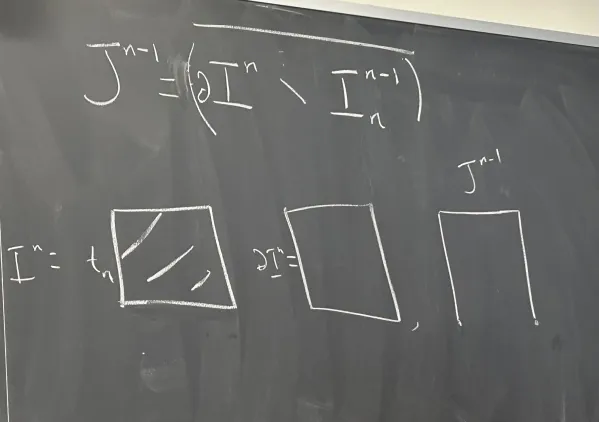
\includegraphics[width=0.5\textwidth]{Figures/horn.png}\]
\end{definition}

From here we construct the relative homotopy group as
\begin{definition}
   For $n \geq 1$, we define $\pi_n(X, A, x_0) = \{f: (I^n, \partial I^n, J^{n-1}) \to (X, A, x_0)\}/\sim$, where $\sim$ is homotopy through maps of the same sort - in other words, $H_t: (I^n, \partial I^n, J^{n-1}) \to (X, A, x_0)$ for all $t$.\\

   From here, we define a sum operation on $\pi_n(X, A, x_0)$ as follows - let $f, g: (I^n, \partial I^n, J^{n-1}) \to (X, A, x_0)$, we can define $f + g$ by juxtaposing their diagrams in the following sense:
   \[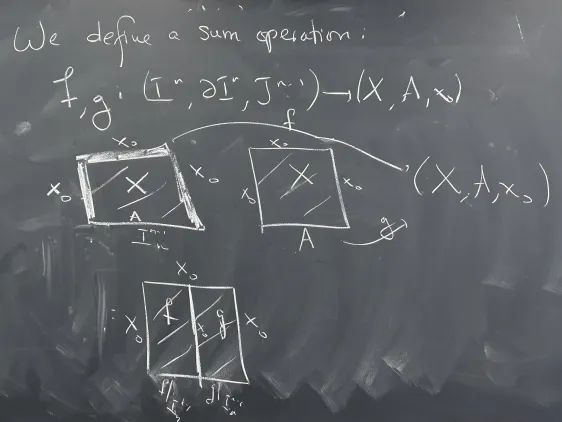
\includegraphics[width=0.6\textwidth]{Figures/relative_pin.png}\]
\end{definition}

One can check the following that we will not do:
\begin{proposition}
    For the relative homotopy group $\pi_n(X, A, x_0)$:
    \begin{enumerate}
        \item The operation $+$ is well-defined up to homotopy. In other words, $[f + g]$ depends only on $[f], [g] \in \pi_n(X, A, x_0)$.
        \item $\pi_n(X, A, x_0)$ is a pointed set if $n = 1$, is a group if $n = 2$, and is an abelian group if $n > 2$.
    \end{enumerate}
\end{proposition}

Here are is another description of the relative homotopy groups.
\begin{proposition}
    We have the isomorphism
    \[\pi_n(X, A, x_0) = \cong [(D^n, S^{n-1}, s_0), (X, A, x_0)]_*.\]
    Recall that $\pi_n(X, x_0) \cong \pi_{n-1}(\Omega X, c_{x_0})$. Let $\Omega_A X = \{\gamma: I \to X\ |\ \gamma(0) = x_0, \gamma(1) \in A\}$. Now it is true that
    \[\pi_n(X, A, x_0) \cong \pi_{n-1}(\Omega_A X, c_{x_0}).\]
    This isomorphism explains why $\pi_1(X, A, x_0)$ is not a group and $\pi_2(X, A, x_0)$ is typically not abelian - this is because $\Omega_A X$ is not necessarily an $H$-space.
\end{proposition}

\begin{lemma}\label{lem::relative_pin_null}
     $f: (D^n, S^{n-1}, s_0) \to (X, A, x_0)$ represents $0 \in \pi_n(X, A, x_0)$ if and only if \ul{$f \simeq g$, rel $S^{n-1}$}, where
     \[g: (D^n, S^{n-1}, s_0) \to (A, A, x_0).\]
     In other words, it is homotopic rel $S^{n-1}$ to a map whose image is in $A$. By homotopic rel $S^{n-1}$, we mean that we have a homotopy $H_t: (D^n, S^{n-1}, s_0) \to (X, A, x_0)$ with the additional constraint that the entire homotopy fixes what it does on $S^{n-1}$, ie.
     \[H_t(x) = f(x), \forall t, \forall x \in S^{n-1}.\]
\end{lemma}

\begin{proof}
    The converse is obvious. If we have such homotopy rel $S^{n-1}$, it clearly gives an equivalence between $[f] = [g]$ in $\pi_n(X, A, x_0)$, where we have $g: D^n \to A$. This implies that $g \simeq c_{x_0}$ since $D^n$ is contractible.\\

    For the forward direction, suppose $[f] = 0$ in $\pi_n(X, A, x_0)$. Then there exists a homotopy $H: D^n \times I \to X$ where $H_t: (D^n, S^{n-1}, s_0) \to (X, A, x_0)$ where $H_0 = f$ and $H_1 = c_{x_0}$. A pictorially representation of this homotopy is to think of the ``solid soup can" as follows:
    \[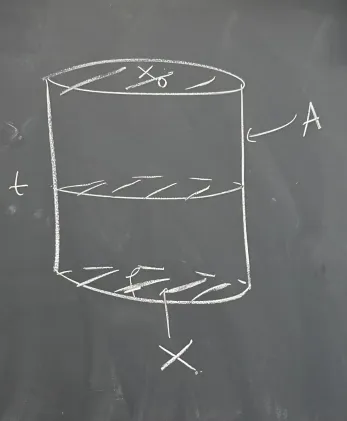
\includegraphics[width=0.2\textwidth]{Figures/soup_can.png}\]
    What we will do now is we will ``push the bottom of the soup can" up. More rigorously, there exists a deformation retraction that removes $D_0 = D^n \times \{0\}$ to $D_1 = D^{n} \times \{1\} \cup S^{n-1} \times I$, which are homeomorphic to $D^n$. Let $D_t$ be the intermediate level disks that rise up. When we perform this deformation retract, the object $D_t$ at the intermediate times are also homeomorphic to disks $D^n$:
    \[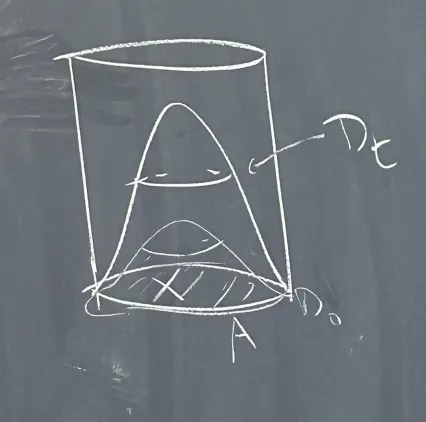
\includegraphics[width=0.3\textwidth]{Figures/soup_can_dt.png}\]
    In particular, for each $t$ we have that $\partial D_t = S^{n-1} \times \{0\}$. Now we consider for each $t$, the function
    \[H|_{D_t}: (D_t, \partial D_t, s_0) \to (X, A, x_0)\]
    Here, $H|_{D_t}$ NEVER moves the boundary, so it is rel $S^{n-1}$. This is our desired homotopy.
\end{proof}

Here are some more facts on relative homotopy groups that we will not prove.
\begin{proposition}
    We have the following:
    \begin{enumerate}
        \item $\pi_n(X, A, x_0)$ is functorial on $T_{2*}$.
        \item $\pi_n(X, A, x_0) \cong \pi_n(X, A, x_1)$ if there exists a path from $x_0$ to $x_1$ lying in $A$.
    \end{enumerate}
\end{proposition}

\begin{proposition}
    Given $(X, A, x_0) \in T_{2*}$, there exists a long exact sequence
% https://q.uiver.app/#q=WzAsNyxbMCwxLCJcXHBpX24oQSwgeF8wKSJdLFsxLDEsIlxccGlfbihYLCB4XzApIl0sWzIsMSwiXFxwaV9uKFgsIEEsIHhfMCkiXSxbMCwyLCJcXHBpX3tuLTF9KEEseCBfMCkiXSxbMSwyLCJcXHBpX3tuLTF9KFgsIHhfMCkiXSxbMiwyLCIuLi4iXSxbMiwwLCIuLi4iXSxbMCwxLCJpXyoiLDJdLFsxLDIsImpfKiJdLFsyLDMsIlxccGFydGlhbCIsMl0sWzMsNCwiaV8qIiwyXSxbNCw1LCJqXyoiXSxbNiwwXV0=
\[\begin{tikzcd}
	&& {...} \\
	{\pi_n(A, x_0)} & {\pi_n(X, x_0)} & {\pi_n(X, A, x_0)} \\
	{\pi_{n-1}(A,x _0)} & {\pi_{n-1}(X, x_0)} & {...}
	\arrow[from=1-3, to=2-1]
	\arrow["{i_*}"', from=2-1, to=2-2]
	\arrow["{j_*}", from=2-2, to=2-3]
	\arrow["\partial"', from=2-3, to=3-1]
	\arrow["{i_*}"', from=3-1, to=3-2]
	\arrow["{j_*}", from=3-2, to=3-3]
\end{tikzcd}\]
    Here $i: (A, x_0) \to (X, x_0)$ is the inclusion and $j: (X, x_0, x_0) \to (X, A, x_0)$ is also the inclusion. The boundary map $\partial$ is given as follows - if $f: (I^n, \partial I^n, J^{n-1}) \to (X, A, x_0)$, we send $\partial f$ to the restriction of $f$ to $I^{n-1}_n$. Schematically, we restrict to the bottom face here:
    \[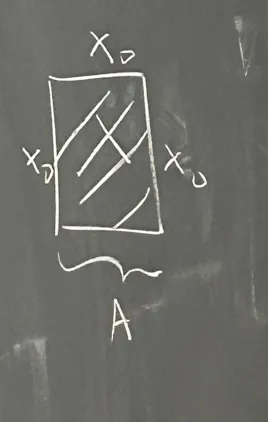
\includegraphics[width=0.2\textwidth]{Figures/bottom_face.png}\]
\end{proposition}

\begin{remark}
    In the world of homology, for nice pairs $(X, A)$ (when $A \to X$ is a cofibration), Excision tells us that $H_n(X, A) \cong \Tilde{H}_n(X, A)$. This is part of what makes homology so nice. However, $\pi_n(X, A, x_0)$ is not typically isomorphic to $\pi_n(X/A, x_0)$. In other words, there is no excision for homotopy groups.
\end{remark}

\begin{proof}
    We only check a few places and leave the rest as exercises. For exactness at $\pi_n(X, x_0)$, we have
    \begin{enumerate}
        \item We see that $j_* \circ i_* = (j \circ i)_*$. The map $j \circ i$ is given by
        \[(A, x_0, x_0) \to (X, x_0, x_0) \to (X, A, x_0).\]
        Hence if $f: (I^n, \partial I^n) \to (A, x_0)$ is a map, then $j \circ i \circ f$ has image in $A$. By Lemma~\ref{lem::relative_pin_null}, this means that $j \circ i \circ f$ represents $0$ in $\pi_n(X, A, x_0)$. Hence, $\operatorname{im}(i_*) \subset \ker(j_*)$.
        \item Now suppose $f: (I^n, \partial I^n) \to (X, x_0)$ is a map such that $j \circ f$ is $0$ in $\pi_n(X, A, x_0)$. Then by Lemma~\ref{lem::relative_pin_null}, $f$ is homotopic rel $S^{n-1}$ to $g$, where $\operatorname{im}(g) \subseteq A$. Hence we have that $[f] = [g]$, and $[g]$ comes from $\pi_n(A, x_0)$ by $i_*$.
    \end{enumerate}
    For exactness at $\pi_n(X, A, x_0)$, we have that
    \begin{enumerate}
        \item We claim $\partial \circ j_* = 0$ - indeed, let $f: (I^n, \partial I^n, J^{n-1}) \to (X, x_0, x_0)$, then $j \circ f$ becomes a map 
        \[(I^n, \partial I^n, J^{n-1}) \to (X, x_0, x_0) \to (X, A, x_0).\]
        Hence we see that $j \circ f|_{I^{n-1}_n}$ has its image in $x_0$, so it represents $0$ in $\pi_{n-1}(A, x_0)$.
        \item Conversely, suppose $f: (I^n, \partial I^n, J^{n-1}) \to (X, A, x_0)$ such that $\partial f = f|_{I^{n-1}_n}$ represents $0$ in $\pi_{n-1}(A, x_0)$. Hence, there exists a homotopy $H$ from $f|_{I^{n-1}_n}$ to $c_{x_0}$. This homotopy lies in $A$.\\

        Now we consider the diagram
        \[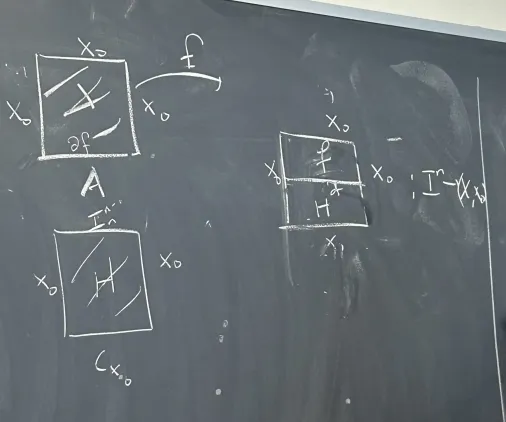
\includegraphics[width=0.5\textwidth]{Figures/homotopy_exact.png}\]
    \end{enumerate}
\end{proof}

\subsection{Weak Homotopy Equivalence}
Before the lecture ends, we will make some definitions.

\begin{definition}
    We have that
    \begin{enumerate}
        \item $(X, x_0)$ is called $n$-connected if $\pi_n(X, x_0) = 0$ for $k \leq n$. In particular, $0$-connected means path-connected, and $1$-connected means simply connected. Note in particular that $n$-connected implies $0$-connected, so this definition becomes independent of base points.
        \item $(X, A, x_0)$ is $n$-connected if $\pi_{k}(X, A, x_0) = 0$ for $k \leq n$.
        \item A map $f: X \to Y$ is a \textbf{weak homotopy equivalence} if the induced map $f_*: \pi_n(X, x_0) \to \pi_n(Y, f(x_0))$ is an isomorphism for all $x_0 \in X$.
    \end{enumerate}
\end{definition}

It is not true that every weak homotopy equivalence is a homotopy equivalence.
\begin{example}
    Let $C$ be the Cantor set and let $C'$ be the Cantor set with the discrete topology. There is a canonical map $C^{\delta} \to C$,  this is an isomorphism for all homotopy groups, but there is no way we can get a map backwards.
\end{example}

\begin{theorem}[Whitehead's Theorem]
    If $f: X \to Y$ is a map between CW-complexes and is a weak homotopy equivalence, then $f$ is a homotopy equivalence.
\end{theorem}

\newpage
\section{Lecture September 19th, 2024}

\subsection{The 3 Basic Theorems of Homotopy Theory}

Today we will be proving Whitehead's theorem. Next week the instructor will be away, but Tony will substitute for him. We will first list a proposition.

\begin{proposition}\label{prop::null_hom_equiv}
    For a space $X$, the following are equivalent:
    \begin{enumerate}
        \item (a) Every map $f: S^k \to X$ is (free) homotopic to a constant map.
        \item (b) Every map $f: S^k \to X$ extends to a continuous map $\Tilde{f}: D^{k+1} \to X$.
        \item (c) $\pi_k(X, x_0) = 0$ for all $x_0 \in X$.
    \end{enumerate}
\end{proposition}

Exercise. Homework due next Thursday. The geometric intuition for (1) implies (2) for the first equivalence statememnts is that a null-homotopy $f: S^k \times I \to X$ factors through $S^k \times I/\sim$ where we identify $(s, 1) \sim (s', 1)$ for all $s \in S^k$. This is now a map from the cone of $S^k$ (ie. $D^{k+1}$) to $X$.

\begin{proof}[Added After Class Is Over]
    For (a) implies (b): Suppose $f: S^n \to X$ is homotopic to a constant map at $x \in X$. This means that there is a continuous function $H: S^n \times I \to X$ such that $H(s, 0) = f(s)$ and $H(s, 1) = x$ for all $s \in S^n$. We define a continuous function $F: CS^n = S^n \times I/S^n \times \{1\} \to X$ as follows:
    \[F(s, t) = H(s, t), t < 1, F([(s, 1)]) = x.\]
    In other words, $F$ is the same as $H$ outside the cone point and $F$ sends to cone point to $x$. By the universal property of quotient maps, $F$ would in fact be continuous (in fact, while we defined $F$ rather explicitly, it can also be seen as the unique map $F: CS^n \to X$ that factors $H$, ie. $F \circ q = H$ where $q$ is the quotient map into the cone - it is a standard fact in point set topology that if $g$ is quotient and $f \circ g$ is continuous, then $f$ is continuous).\\

    Now there is an obvious homeomorphism $h$ from $D^{n+1}$ to $CS^n$ that the ``identity" on $S^n = \partial D^{n+1}$ (sending $s \in S^n$ to $(s, 0) \in CS^n$). We then see that $F \circ h: D^{n+1} \to X$ is the desired continuous extension of $f$ since for all $s \in S^n$, $F \circ h(s) = F(s, 0) = H(s, 0) = f(s)$.\\

    For (b) implies (c): Let $f: (S^n, s_0) \to (X, x_0)$ be a based map sending $s_0$ to $x_0$. From (b), we know that $f$ extends to a map $\Tilde{f}: D^{n+1} \to X$. Write an element $(r, \theta) \in D^{n+1}$ in terms of the polar form ($\theta \in S^{n}$ and $r \in (0, 1]$. When $r = 0$, just denote it as the origin), there is an obvious homeomorphism $h$ from $D^{n+1}$ to $C S^{n} = S^n \times I/S^n \times 1$ given by sending $(r, \theta)$ to $(1-\theta, r)$ and the origin to the cone point. We can then construct twp map:
    \[F: CS^n \to X, F = \Tilde{f} \circ h^{-1}.\]
    \[H: S^n \times I \to X, H = F \circ q - q \text{ is the quotient map to the cone}.\]
    Now, we are not actually done. This is because we want to choose a $\Tilde{f}$ such that $H(s_0, t) = x_0$ for all $t$. To do this, it suffices for us to construct a continous function $g: D^{n+1} \to D^{n+1}$ such that $g(r, s_0) = s_0$ for all $r \in (0, 1]$, $g(0) = s_0$, and $g$ is the identity on $S^n$. Then if we replace $\Tilde{f}$ with $\Tilde{f} \circ g$, then this will give a based homotopy $H$ between $f$ and the constant map at $x_0$. From there we can conclude that $\pi_n(X, x_0) = 0$.\\

    To see that this function $g$ exists. For each $s \in S^{n+1}$, consider the path $\gamma_s$ from $\gamma_s(0) = s$ to $\gamma_s(1) = s_0$ that is the straight line segment (according to stereographic projection). We notice that $\gamma_{s_0}$ is the constant path. Now, we may construct $g$ as for all $r \in (0, 1]$ and $\theta \in S^{n+1}$
    \[g(r, \theta) = \gamma_{\theta}(1-r)\]
    \[g(0) = s_0.\]
    This is a continuous function that satisfies the constraints we required.

    For (c) implies (a): Suppose $\pi_n(X, x_0) = 0$ for all $x_0 \in X$. Let $f: S^n \to X$ be a continuous function. Let $p \in S^n$ and $f(p) \in X$, we know $\pi_n(X, f(p)) = 0$, so $f$ is based homotopic to a constant map, so it is in particular homotopic to a constant map.
\end{proof}

\begin{proposition}
    For a pair of spaces $(X, A)$, the following are equivalent:
    \begin{enumerate}
        \item (a) Every map $(D^k, \partial D^k) \to (X, A)$ is homotopic rel $\partial D^k$ (ie. $f_t|_{\partial D^k} = f|_{\partial D^k}$) to a map $D^k \to A$.
        \item (b) Every map $f: (D^k, \partial D^k) \to (X, A)$ is homotopic through maps $f_t: (D^k, \partial D^k) \to (X, A)$ to a map $f_1: D^k \to A$.
        \item (c) Every map $f: (D^k, \partial D^k) \to (X, A)$ is homotopic through maps $f_t: (D^k, \partial D^k) \to (X, A)$ to a constant map $f_1: D^k \to A$.
        \item (d) $\pi_k(X, A, x_0) = 0$ for all $x_0 \in A$.
    \end{enumerate}
\end{proposition}

\begin{proof}
    For (a) implies (b), from (a) we know that there is a map $H: D^n \times I \to X$ such that $H(x, 0) = f(x)$, $H|_{\partial D^n \times I} = f|_{\partial D^n}$, and $H(x, 1) = g(x)$. Now in particular, for each $x \in \partial D^n$, $H(x, t) = f|_{\partial D^n}(x) \in A$, so each map $x \mapsto H(x, t)$ is a map of pairs $(D^n, \partial D^n) \to (X, A)$. Thus, this gives a homotopy from $f$ to $g$ through ``such maps" outlined in (b).\\
    
    For (b) implies (c), suppose $f: (D^n, \partial D^n) \to (X, A)$ is a map of pairs. From (b), we know that there is a map $H: D^n \times I \to X$  such that $H(x, 0) = f(x)$, $x \mapsto H(x, t)$ sends $\partial D^n$ into $A$ and $H(x, 1) = g(x)$, where $g: D^n \to A$. Now, since $g: D^n \to A$ is continuous and $D^n$ is contractible, we know $g$ is null-homotopic and is homotopic to a constant map. Let $E: D^n \times [0, 1] \to A$ be this homotopy, where $E(x, 0) = g(x)$ and $E(x, 1)$ is constant for all $x$. Now consider the map $F: D^n \times [0, 1] \to X$ defined by
    \[F(x, t) = \begin{cases}
        H(x, 2t), t \in [0, \frac{1}{2}]\\
        E(x, 1 - 2t), t \in [\frac{1}{2}, 1]
    \end{cases}.\]
    This is continuous by the glueing lemma. The maps $x \mapsto H(x, 2t), t \in [0, \frac{1}{2}]$ are map of pairs $(D^n, \partial D^n) \to (X, A)$ as we checked before. The maps $x \mapsto E(x, 1-2t), t \in [\frac{1}{2}, 1]$ are also map of pairs $(D^n, \partial D^n) \to (X, A)$ since the image of $E$ lies in $A$ completely. Thus, $F$ gives a desired homotopy of $f$ to a constant map through such maps.\\

    We skip (c) implies (d) now and look at the case for (d) implies (a) first.\\

    For (d) implies (a), we actually proved this as a lemma during Lecture September 17th, 2024. For completeness I will copy the exact proof written in lecture.
    \begin{lemma}\label{lem::relative_pin_null}
     $f: (D^n, S^{n-1}, s_0) \to (X, A, x_0)$ represents $0 \in \pi_n(X, A, x_0)$ if and only if \ul{$f \simeq g$, rel $S^{n-1}$}, where
     \[g: (D^n, S^{n-1}, s_0) \to (A, A, x_0).\]
     In other words, it is homotopic rel $S^{n-1}$ to a map whose image is in $A$. By homotopic rel $S^{n-1}$, we mean that we have a homotopy $H_t: (D^n, S^{n-1}, s_0) \to (X, A, x_0)$ with the additional constraint that the entire homotopy fixes what it does on $S^{n-1}$, ie.
     \[H_t(x) = f(x), \forall t, \forall x \in S^{n-1}.\]
\end{lemma}

\begin{proof}[Added After Class Is Over]
    The converse is obvious. If we have such homotopy rel $S^{n-1}$, it clearly gives an equivalence between $[f] = [g]$ in $\pi_n(X, A, x_0)$, where we have $g: D^n \to A$. On the other hand, $g \simeq c_{x_0}$ through maps of the the form $(D^n, S^{n-1}, p) \to (A, A, x_0) \subseteq (X, A, x_0)$ since $D^n$ is contractible.\\

    For the forward direction, suppose $[f] = 0$ in $\pi_n(X, A, x_0)$. Then there exists a homotopy $H: D^n \times I \to X$ where $H_t: (D^n, S^{n-1}, s_0) \to (X, A, x_0)$ where $H_0 = f$ and $H_1 = c_{x_0}$. A pictorially representation of this homotopy is to think of the ``solid soup can" as follows:
    \[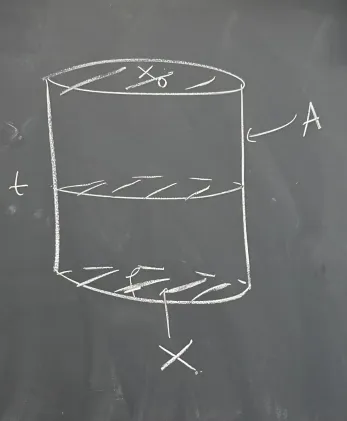
\includegraphics[width=0.2\textwidth]{Figures/soup_can.png}\]
    What we will do now is we will ``push the bottom of the soup can" up. More rigorously, there exists a deformation retraction that moves $D_0 = D^n \times \{0\}$ to $D_1 = D^{n} \times \{1\} \cup S^{n-1} \times I$, which are homeomorphic to $D^n$. Let $D_t$ be the intermediate level disks that rise up. When we perform this deformation retract, the object $D_t$ at the intermediate times are also homeomorphic to disks $D^n$:
    \[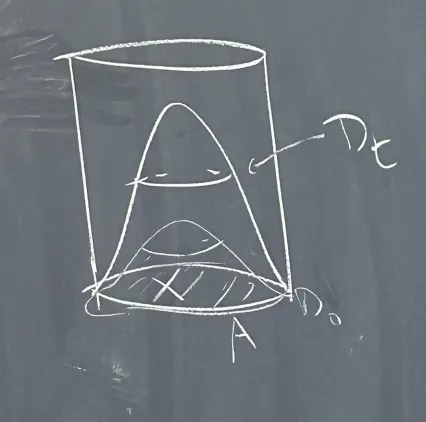
\includegraphics[width=0.3\textwidth]{Figures/soup_can_dt.png}\]
    In particular, for each $t$ we have that $\partial D_t = S^{n-1} \times \{0\}$. Now we consider for each $t$, the function
    \[H|_{D_t}: (D_t, \partial D_t, s_0) \to (X, A, x_0)\]
    Here, $H|_{D_t}$ NEVER moves the boundary, so it is rel $S^{n-1}$. This is our desired homotopy.
\end{proof}

Let us now come back to (c) implies (d). Suppose $f: (D^n, \partial D^n, p) \to (X, A, x_0)$ is a map of pairs with $f(p) = x_0 \in A$. From (c), we know  $f$ is homotopic through maps of pairs $(D^n, \partial D^n) \to (X, A)$ to a constant map $D^n \to A$ to some constant $c$. The image of $f$ is path-connected because $D^n$ is path-connected, so this $c$ must be in the same path-component as $x_0$. Thus, we can extend whatever homotopy this is by a path from $c$ to $x_0$, so we without loss have that $f$ is homotopic through maps of pairs $(D^n, \partial D^n) \to (X, A)$ to the constant map at $x_0 \in A$. \underline{Let $H$ denote this homotopy}. \\

To show that $f$ represents $0$ in $\pi_n(X, A, x_0)$, we need a homotopy $F$ through maps of pairs $(D^n, \partial D^n) \to (X, A)$ to the constant map at $x_0 \in A$ that also fixed the based point $p$ (in other words $t \mapsto F(p, t)$ is constant with value $x_0$).

Let us now consider the exact same procedure outlined in the forward direction of Lemma~\ref{lem::relative_pin_null}, ie. we construct $H|_{D_t}: (D_t, \partial D_t, s_0) \to (X, A, x_0)$ the same way. $H|_{D_t}$ is a now a homotopy rel $\partial D^n$ from $f$ to NOT THE CONSTANT MAP but a map $g: D^n \to A$ (since everything at the $D^{n} \times \{1\}$ and on $\partial D^n \times [0, 1]$ gets sent to $A$). Note that $g(p) = f(p)$ since $p \in \partial D^{n})$. This is good enough because we can find a base homotopy $E: D^n \times [0, 1] \to A$ from $g$ to the constant map at $x_0$ with $E(p, t) = x_0$ for all $x_0$.\\

Combining the homotopy $H|_{D_t}$ and $E$ now gives us a desired homotopy through maps of pairs $(D^n, \partial D^n, p) \to (X, A, x_0)$ that shows $f$ represents $0$ in the relative homotopy group.
\end{proof}
We will first state the 3 basic theorems of homotopy theory.

\begin{theorem}[Whitehead's Theorem]
   Let $X, Y$ be CW complexes. Let $f: X \to Y$ be a map inducing an isomorphism $f_*: \pi_n(X, x_0) \to \pi_n(Y, f(x_0))$ for all $x_0 \in X$ and for all $n$, then $f$ is a homotopy equivalence. Furthermore, if $f: X \to Y$ is the inclusion of a subcomlex, then $Y$ deformation retracts onto $X$.
\end{theorem}

\begin{remark}
    It is not enough that the homotopy groups of $X$ and $Y$ are isomorphic for them to be homotopy equivalent. You need a map that induces an isomorphism of their homotopy groups! For example, we can take $X = S^2 \times \Rbb P^3$ and $Y = S^3 \times \Rbb P^2$. They are both double covered by $S^2 \times S^3$ and hence have the same $\pi_n$ for $n \geq 2$. They also have the same $\pi_1$ and $\pi_0$. However, they are not homotopy equivalent because they have different $H_{5}$ over $\Zbb$. This is because $\Rbb P^2 \times S^3$ is not orientable, so $H_5(\Rbb P^2 \times S^3) = 0$,  but $\Rbb P^3 \times S^2$ is orientable and closed, so $H_5(\Rbb P^3 \times S^2) \neq 0$.
\end{remark}

\begin{theorem}[Cellular Approximation]
    Let $X, Y$ be CW complexes. Suppose $f: X \to Y$ is (only) a continuous map, then $f$ is homotopic to a map $g: X \to Y$, where $g$ is cellular. Here, by cellular, we mean that $g$ takes the $n$-skeleton of $X$ to the $n$-skeleton of $Y$, ie.
    \[g(X^n) \subseteq Y^n.\]
    Moreover, if $(X, A)$ is a cellular pair and $f$ is already cellular on $A$, then we can take the homotopy to $g$ relative to $A$ (ie. $g$ extends $f|_{A}$).
\end{theorem}

\begin{corollary}
    The cellular approximation admits a purely topological proof for $\pi_k(S^n) = 0$ for $k < n$.
\end{corollary}

\begin{proof}
    We know that $S^n = e^0 \cup e^n$ and $S^k = e^0 \cup e^k$. Let $f: S^k \to S^n$ be a continuous map, the cellular approximation theorem implies $f$ is homotopic to a cellular map $g: S^k \to S^n$. However, since $g$ is a cellular map and $k < n$, $g(e^0 \cup e^k) = e^0 \in S^n$. Thus, $g$ has to be constant. Thus, we conclude that $\pi_k(S^n) = 0$.
\end{proof}

\begin{theorem}[CW Approximation]
    Given any $X$, there exists $Y$ a CW complex and a map $f: Y \to X$ that is a weak homotopy equivalence.
\end{theorem}

\begin{remark}
    The statement of CW Approximation is really a statement about derived functors.
\end{remark}

\subsection{Proof of Whitehead's Theorem}

\begin{lemma}[Compression Lemma]
    Let $(X, A)$ be a CW-pair ($A$ is a subcomplex of $X$) and $(Y, B)$ with $B \neq \emptyset$ be any pair. For any $n$ such that $X \setminus A$ has $n$-cells and $\pi_n(Y, B, y_0) = 0$ for all $y_0 \in Y$, then we have that - Any map $f: (X, A) \to (Y, B)$ is homotopic rel $A$ to a map $g: X \to B$.
\end{lemma}

\begin{remark}
    In this class, we will use the word cellular pair and CW-pair interchangeably. The intuition of this lemma is we are assuming the topological complexities of $(X, A)$ and $(Y, B)$ are ``orthogonal" in dimensions, which provides a suitable constraint on the homotopy class of possible map between them.
\end{remark}

\begin{proof}
Assume inductively that $f$ has been homotoped to take $X^{k-1}$ to $B$. We will let the reader think about what happens to the $0$-skeleton. If $\Phi: e^k \to X \setminus A$ exists (if it doesn't exist, we are done) and is the characteristic map of a $k$-cell, then $f \circ \Phi: (D^k, \partial D^k) \to (Y, B)$ can be homotoped rel $\partial D^k$ into $B$ (here we use the assumption $\pi_k(Y, B, y_0) = 0$ if $X \setminus A$ has a $k$-cell and Proposition~\ref{prop::null_hom_equiv}). This homotopy induces a homotopy rel $X^{k-1}$ on $X^{k-1} \cup_{\psi} e^k$ (where $\psi: S^{k-1} = \partial e^k \to X$ is the attaching map). We can do this simultaneously for all $k$-cells while taking the constant homotopy on $A$. This is okay because the characteristic maps send interior of cells to disjoint places, and the only overlaps happen on the boundary, but all the homotopies are rel boundary (on $X^{k-1}$), so they form a well-defined homotopy together.\\

From the discussions above, we obtain a homotopy of $f|_{X^k \cup A}$ to a map to $B$. With some abuse of notation, we call this new map that is homotoped to as $f$. This $f$ has the property that it takes $X^k$ into $B$ and fixes $A$. Now we use the magic of the homotopy extension property (since CW-pairs satisfy the HEP), we can obtain an extension of this homotopy to all of $X$, being $f$ on $X^k \cup A$. This concludes the inductive step.\\

If $X \setminus A$ has cells in finitely dimensions, we can use induction and we are done with the proof. If $X \setminus A$ has cells in infinitely many dimensions, we can perform the k-th homotopy $H_k$ described above on the $k$-skeleton in the time interval $[1 - 2^{-k}, 1 + 2^{-(k+1)}]$ (together they add up to $[0, 1])$, so any finite skeleton is eventually stationary under the homotopies. Hence, we can obtain a well-defined map on $X \times I$. Schematically, let $\undertilde{H_k}$ be the homotopy extension on $X$ obtained from each $H_k$ (that only operates on $X^k \cup A$, then we have a homotopy of the form
\[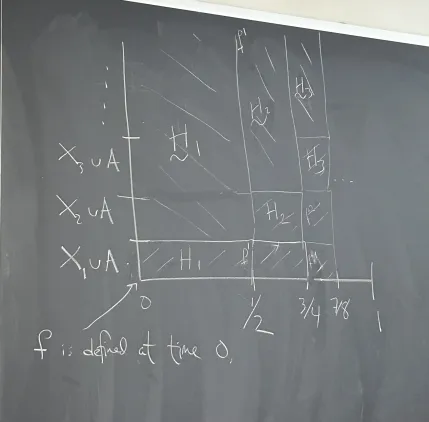
\includegraphics[width=0.5\textwidth]{Figures/infinite_hom_compression.png}\]
They glue together a continuous map by a repeated use of the glueing lemma and gives the homotopy we desire.
\end{proof}

Now we give of a proof of Whitehead's theorem.
\begin{proof}[Proof of Whitehead's Theorem]
    If $f: X \to Y$ is an inclusion of a subcomplex that is an isomorphism on homotopy groups, then we look at $\pi_n(Y, X)$. From the long exact of sequence of homotopy groups, we have
    \[... \to \pi_{n+1}(Y, X) \to \pi_n(X) \to \pi_n(Y) \to \pi_n(Y, X) \to \pi_{n-1}(X) \to \pi_{n-1}(Y) \to ...\]
    Hence $f: X \to Y$ is an isomorpjism on homotopy groups, exactness implies that $\pi_n(X, Y) = 0$ for all $n$. Now we can apply the compression lemma to the map $1: Y \to Y$ (the identity map on $Y$), which implies $1: Y \to Y$ is homotopic rel $X$ to a map $g: Y \to X$, which is exactly what deformation retract means.\\

    In general, if $f: X \to Y$ is a weak homotopy equivalence. Let us take the mapping cylinder $\operatorname{Cyl}(f)$ of $f$. Recall there is an obvious deformation retract of $\operatorname{Cyl}(f)$ onto $Y$ and there is a decomposition of $f$
    \[X \to \operatorname{Cyl}(f) \simeq Y\]
    where $X \to \operatorname{Cyl}(f)$ is a cofibration and $\operatorname{Cyl}(f) \to Y$ is a homotopy equivalence. In particular, functoriality tells us that the inclusion map $X \to \operatorname{Cyl}(f)$ is a weak homotopy equivalence, which implies that
    \[\pi_n(\operatorname{Cyl}(f), X) = 0, \forall n.\]
    Then we go back to the previous case and see that $X$ and $Y$ are homotopy equivalent.\\
    
    This argument should have worked except IT IS NOT ALWAYS true that $\operatorname{Cyl}(f)$ is a CW-complex. However, $\operatorname{Cyl}(f)$ is a CW complex whenever $f$ is a cellular map!!! Here, we can use Cellular Approximation to replace $f$ by a cellular map up to homotopy.
\end{proof}

\subsection{Eilenberg-Maclane Spaces}

\begin{lemma}
    If $(X, A)$ is a CW-pair, $f: A \to Y$ is a map, and $Y$ is path-connected.
    
    Suppose $\pi_{n-1}(Y) = 0$ for all $n$ such that $X - A$ has no n-cells, then $f$ can be extended to a map $\Tilde{f}: X \to Y$ such that $\Tilde{f}|_{A} = f$.
\end{lemma}

\begin{definition}
    Let $n \in \Nbb$, let $\pi$ be a group if $n = 1$ and an abelian group if $n \geq 2$. A $K(\pi, n)$ (also called an Eilenberg-Maclance space) is a space $X$ such that
    \[\pi_k(X) = \begin{cases}
        \pi, k = n\\
        0, k \neq n
    \end{cases}.\]
    If there exists a $K(\pi, n)$, we can always take it to be a CW-complex by the CW approximation theorem.
\end{definition}

\begin{example}
    Here are some fun examples of Eilenberg-Maclane spaces
    \begin{enumerate}
        \item $S^1$ is $K(\Zbb, 1)$.
        \item $S^1 \times S^1$ is $K(\Zbb^2, 1)$.
        \item Being $K(\pi, 1)$ is the same as being aspherical on CW-complexes.
        \item $K(\Zbb, 2) = \Cbb P^{\infty}$.
        \item $K(\Zbb/2, 2) = \Rbb P^{\infty}$.
    \end{enumerate}
\end{example}

\begin{proposition}
    Let $X$ and $Y$ are two CW-complexes which are both $K(\pi, n)$, then $X$ is homotopy equivalent to $Y$.
\end{proposition}

\begin{proof}
    Next lecture.
\end{proof}

\newpage
\section{Lecture September 24th, 2024}

\subsection{Cellular Approximation Theorem}
Let us quickly recall the definition of a CW complex again.
\begin{definition}
    A CW complex is a Hausdorff topological space $X$ such that
    \[X = \bigsqcup_{q = 0}^\infty \bigsqcup_{i \in I_q} e_i^q,\]
    where each $e_i^q \subset X$ is a subset and for all $q, i$, there exists continuous maps $\varphi_i^q: D^q \to X$ continuous such that $\varphi_i^q$ restricted to the interior is a homeomorphism onto $e_i^q$ satisfying the axioms
    \begin{itemize}
        \item (c) (Closure finiteness) - $e^q_i$ belongs in the union of finitely many cells of dimension $< q$.
        \item (w) (Weak Topology) - we say $F \subset X$ is closed if and only if $F \cap \overline{e_i^q}$ is closed for all $q, i$.
    \end{itemize}
\end{definition}

\begin{definition}
    Let $X, Y$ be CW complexes and $f: X \to Y$ is a continuous map. We say $f$ is a \textbf{cellular map} if for every cell $e_i^q \subseteq X$, $f(e_i^q) \subseteq \bigcup (\text{cells of $Y$ of dimensions $\leq q$})$.
\end{definition}

\textbf{Notation:} If $X$ is a CW complex, we write the subcomplex $X^q$ (the $q$-skeleton) as the union of all cells in $X$ of dimension $\leq q$. 

\begin{remark}
  Let $X^{-1}$ be the empty set, $\{X^q - X^{q-1}\}_{q \geq 0}$ breaks $X$ into a union of (Whitney) strata. In this sense, $X^q$ may be viewed as the closure of the strata.
\end{remark}

\begin{theorem}[Cellular Approximation Theorem]
    If $X, Y$ are CW complexes and $f: X \to Y$ is any continuous map. 
    \begin{enumerate}
        \item There exists $g: X \to Y$ cellular such that $f \sim g$.
        \item (Slightly Stronger): If $A \subset X$ is a CW subcomplex and $f: X \to Y$ is a continuous map such that $f|_{A}: A \to Y$ is cellular, then we can choose $g$ such that $g$ and $f$ are homotopic rel $A$ (ie. the homotopy is stationary on $A$).
    \end{enumerate}
\end{theorem}

\textbf{Notation:} If $A \subset X$ is a subspace in a topological space, $f, g: X \to Y$ are continuous maps such that $f|_{A} = g|_{A}$, then $f \sim g$ with a homotopy stationary on $A$ is denoted as ``$f \sim g$ rel A".

\begin{proof}
    We prove Statement (2), which directly implies Statement (1).\\
    
    We first proceed by induction on $n$ equal to the dimension of the cells. Suppose $A \subset X$ is a subcomplex and $f: X \to Y$ restricts to a cellular map on $A$. Suppose by induction we have managed to make sure that $f$ has been homotoped rel $A$ to be cellular on $X^{n-1} \cup A \to Y$, then we want to make it also cellular on $X^{n} \cup A \to Y$.\\

    Let $e^n \subset X - A$ be a $n$-cell that is not in $A$. If no such $e^n$ exist, we are done. Otherwise, $\overline{e^n}$ is compact by the closure finiteness axiom, and $f(\overline{e^n}) \subset Y$ is also going to be compact. Hence, $f(\overline{e^n})$ is contained in the union of finitely many cells of $Y$. Hence we have a well-defined number $q$ that is the maximum dimension of a cell of $Y$ that meets $f(\overline{e^n})$. Let $e^q$ be one such cell.\\

    If $q \leq n$, we are done, because the map $f: X^{n-1} \cup A \cup e^n \to Y$ is already cellular. If $q > n$, then we want to show that $f: X^n \cup A^n \cup e^{n} \to Y$ is homotopic rel $A^n \cup X^{n-1}$ to a map $X^{n1} \cup A^n \cup e^n \to Y$ which is cellular. To prove this, we will require the use of the Missing Point Lemma (see Lemma~\ref{lem::missing_pt}).\\

    Assuming this holds, since $g(e^n)$ misses some point $p \in e^q$, then we have a (radial) deformation retraction $r_t: Y - p \to Y - e^q$. Composing $r_t$ with $f$ gives a homotopy from $f$ to $g$ which is rel $(X^{n-1} \cup A^n)$ such that $g(e^n) \subseteq \partial \overline{e^q}$. Hence, we obtain a new map $g$ on $X^{n-1} \cup A^n \cup e^n$ (homotopic to $f$ relative to $(X^{n-1} \cup A^{n}$) such that $\operatorname{Im}(g)$ misses $e^q$. After finitely many steps, we can do this repeatedly for obtain a map $g$ miss all the higher dimensional cells.\\

    We can now repeat this for all $n$-dimensional cells of $X$, for which we get a homotopic map rel $X^{n-1} \cup A^n$, such that $g: X^n \cup A^n \to Y$ is cellular. Now we invokve the fact that CW pairs have the homotopy extension property to get a homotopy $g: X \to Y$ such that $f \sim g$ rel $X^{n-1} \cup A^n$ and $g: X^n \to Y$ is cellular.

    \begin{theorem}[Borsuk's Theorem]
    If $X$ is a CW complex and $A \subset X$ is a subcomplex, $Y$ is any topological space, it satisfies the homotopy extension property (ie. any homotopy $h_t: A \to Y$ extend to $H_t: X \to Y$).
\end{theorem}

    If $X$ has finite dimensions, then we are done by induction. Otherwise, we get a sequence of maps $g_0, g_1, g_2, ...$ such that 
    \begin{itemize}
        \item $f \sim g_0$ relative to $A$ and $g_0$ is cellular on $X^0$.
        \item $g_0 \sim g_1$ relative to $(X^0 \cup A)$ and $g_1$ is cellular on $X^1$.
        \item ...
        \item $g_{n-1} \sim g_n$ is relative to $X^{n-1} \cup A$ and $g_n: X^n \to Y$ is cellular.
        \item ...
    \end{itemize}
    Now we want to merge these maps to a single homotopy on $X$. This is an accumulation argument. To do this, we perform the $n$-th homotopy (between $g_n$ and $g_{n+1}$) on the interval $[1-\frac{1}{2^n}, 1 - \frac{1}{2^{n+1}}]$. This gives one well-defined homotopy $f \sim g$ relative to $A$ for $t \in [0,1]$. 
\end{proof}

Now we obtain an immediate powerful corollary of Cellular Approximation.
\begin{corollary}
    Suppose $X, Y$ are CW complexes such that $\dim X < q$ and $Y$ is such that $Y^0 = \{*\}$ and have no other cells of dimension $< q$, then any continuous map $f: X \to Y$ is homotopy equivalent to the constant map into $*$.
\end{corollary}

\begin{example}
    Suppose $q < n$, then $[S^q, S^n]$ is trivial by the corollary above.
\end{example}

\subsection{Missing Point Lemma}
\begin{lemma}[Missing Point Lemma]\label{lem::missing_pt}
    Given $f: X^{n-1} \cup A^n \cup e^n \to Y$, we can find $g: X^{n-1} \cup A^n \cup e^n \to Y$ such that $f \sim g$ rel $(X^{n-1} \cup A^n)$ and the image $g|_{e^n}: e^n \to Y$ such that $g(e^n)$ misses some point $p \in e^q$.
\end{lemma}

\begin{proof}[Proof of the Missing Point Lemma]
    It follows from the following standard claim.\\    
\textbf{Claim: } If $e^n$ is an $n$-dimensional cell and $Z$ is a CW complex such that $Z = W \cup e^q$ (attaching $e^q$ to $W$) and $f: e^n \to Z$, then we can find an open ball $D \subset e^n$ and a map $g: e^n \to Z$ so that
    \begin{enumerate}
        \item $f \sim g$ rel $(f^{-1}(W))$
        \item $g(D) \subset e^q$.
        \item $g$ restricted to $D$ is smooth (some argument with Stone-Weierstrass).
        \item Note that this implies that $g(D)$ misses a point of $e^q$ if $q > n$ by Sard's Theorem. 
    \end{enumerate}
The claim indeed follows from the standard techniques of differential topology.\\

The lemma may also be proven with an alternative claim without necessarily appealing to differential topology.\\
\textbf{Claim:} Suppose $Z = W \cup e^q$ again and $f: I^n = [0, 1]^n \to Z$ is continuous, then there exists $\Delta^q \subset e^q$ a simplex and a map $g: I^n \to Z$ such that 
\begin{enumerate}
    \item $f \sim g$ rel $f^{-1}(W)$.
    \item The $g^{-1}(\Delta^q)$ is the finite disjoint union $\bigsqcup_{s \in S} \operatorname{Pol}_s$ where each $\operatorname{Pol}_s$ is a convex polytope in $I^n$ (convex subset which is the intersection of finitely many affine half-spaces in $\Rbb^n$).
    \item $g$ restricted to each polytope in the disjoint union $g^{-1}(\Delta^q)$ is equal to the restriction of a surjective affine linear map.
    \item If $q > n$, then it follows that $S$ is empty and thus $g^{-1}(\Delta^q)$ is empty.
\end{enumerate}
We will instead look at this claim. We can identify $e^q$ with $\Rbb^q$, we can choose closed balls
\[0 \in B_1 \subset B_2 \subset \Rbb^q = e^q.\]
Here $B_1$ has radius $1$ and $B_2$ has raidus $2$, centered at the orgin. If we look at $f^{-1}(B_1) \subset f^{-1}(B_2)$ are compact (since $f$ restricts to a proper map within the cube whose image will have $B_1$ and $B_2$).\\

In particular, by the Heine-Cantor theorem, $f$ is uniformly continuous on $f^{-1}(B_2)$. This IMPLIES that there exists $\delta > 0$ such that for all $x, y \in f^{-1}(B_2)$ with $|x - y| < \delta$ implies $|f(x) - f(y)| < \frac{1}{2}$.\\

We subdivide the cube $I^n$ into cubes of diameter $< \delta$. Now, let
\begin{itemize}
    \item $K_1$ be the union of all small cubes meeting $f^{-1}(B_1)$.
    \item $K_2$ be the union of all small cubes meeting $K_1$.
\end{itemize}
Since we chose the mesh to be small, we have that
\[f^{-1}(B_1) \subset K_1 \subset K_2 \subset f^{-1}(B_2).\]
NOW $K_1$ and $K_2$ are CW complexes with cells that open faces of all dimensions of the small cubes.\\

We can perform inductively on the dimension of cells in barycentric subdivision of cubes in $K_2$ into simplicies (by connecting midpoints on the simplicies). This gives a simplicial complex structure on $K_2$. Let $F: K_2 \to e^q = \Rbb^q$ be the map which is equal to $f$ on the vertices of simplicies and is affine-linear on each face (the values on the vertices indeed uniquely defines the PL map $F$).\\

Now, we choose a cutoff function
\[c: K_2 \to [0, 1]\]
such that $c|_{\partial K_2} = 0$ and $c|_{K_1} = 1$ (Urysohn's Lemma for continuous maps). Then we get a homotopy
\[h_t = (1 - t c) f - t c F\]
where $h_t: K_2 \to e^q$ such that $h_0 = f$, $h_1|_{K_1} = F|_{K_1}$, and $h_t|_{\partial K_2} = f$. We can extend $h_t$ to $H_t: I^n \to Z$ by making it $H_t|_{I^n - K_2} = f$ for all $t$.\\

If $g = H_1$, then $f \sim g$ rel $f^{-1}(W)$ and $g|_{K_1} = F$ is our desired map. We will finish the proof next time.
\end{proof}


\newpage
\section{Lecture September 26th, 2024}

\subsection{Finishing the Missing Point Lemma}
\textbf{Recall:} Last time, we were in the middle of giving a direct proof of the Missing Point Lemma.

\begin{lemma}[Missing Point Lemma]
    Given $f: X^{n-1} \cup A^n \cup e^n \to Y$, we can find $g: X^{n-1} \cup A^n \cup e^n \to Y$ such that $f \sim g$ rel $(X^{n-1} \cup A^n)$ and the image $g|_{e^n}: e^n \to Y$ such that $g(e^n)$ misses some point $p \in e^q$.
\end{lemma}

The lemma reduced the following key statement that we wanted to prove.

\begin{proposition}
Suppose $Z = W \cup e^q$ and $f: I^n = [0, 1]^n \to Z$ is continuous, then there exists $\Delta^q \subset e^q$ a simplex and a map $g: I^n \to Z$ such that 
\begin{enumerate}
    \item $f \sim g$ rel $f^{-1}(W)$.
    \item The $g^{-1}(\Delta^q)$ is the finite disjoint union $\bigsqcup_{s \in S} \operatorname{Pol}_s$ where each $\operatorname{Pol}_s$ is a convex polytope in $I^n$ (convex subset which is the intersection of finitely many affine half-spaces in $\Rbb^n$).
    \item $g$ restricted to each polytope in the disjoint union $g^{-1}(\Delta^q)$ is equal to the restriction of a surjective affine linear map.
    \item If $q > n$, then it follows that $S$ is empty and thus $g^{-1}(\Delta^q)$ is empty.
\end{enumerate}
\end{proposition}

\begin{proof}[Proof Continued]
    Last time, we showed that if $e^q = \Rbb^q$, we can choose subcomplexes $K_1 \subset K_2 \subset I^n$ where $K_i$ are simplicial complexes with simplicies of small diameter, such that
    \[f^{-1}(B_1) \subset K_1 \subset K_2 \subset f^{-1}(B_2),\]
    where $B_1, B_2$ are balls of radius $1, 2$ in the origin in $\Rbb^q$ respectively. Furthermore, we can choose $K_1, K_2$ such that for all $\sigma \in K_2$, $f(\sigma) \subset K_2$ has diameter strictly less than $\frac{1}{2}$.\\

    Using this, we recall that we constructed a homotopy
    \[h_t: K_2 \to e^q = \Rbb^q \subset Z, h_0 = f, h_1|_{K_1} \text{ is linear on all simplicies of $K_1$, and equal to $f$ on vertices}, \]
    \[\text{ and } h_t|_{\partial K_2} \text{ is } f\quad \forall t.\]
    Now, we can construct a homotopy $g_t: I^n \to Z$ such that $g_t|_{K_2} = h_t$ and $g_t|_{I^n - K_2} = f$ (this is rather explicit). Now, we clearly see that $g_t$ is a homotopy between $g_0 = f \sim g \coloneqq g_1$ rel $f^{-1}(W)$. Furthermore, we see that $g|_{K_1} = h_1|_{K_1}$ is linear on simplicies!\\

    The observation is - if we can find a neighborhood $N \ni 0$ that is contained in $B_2$ such that $g^{-1}(N) \subset K_1$, then we are done as $g$ is linear on $K_1$. To check that this holds, we can equivalently find a neighborhood $N \ni 0$ contained in $B_2$ such that $g(I^n - K_1)$ is contained in $Z - N$. Now, we note that since $g$ DOES THE EXACT SAME AS $f$ outside of $e^q$, we actually have that $$g(I^n - K_1) \subset Z - N \iff g(K_2 - K_1) \subset e^q - N.$$

    Now we take some simplex $\sigma$ in $K_2 - K_1$. Now for each vertex $v$ on $\sigma$, since $h_t|_{\partial K_2} = f$, and $f(v)$ is contained in the same ball of radius $1/2$. Call this ball $\operatorname{Ball}_{\sigma}$. Now, $h_t(\operatorname{vertices\ \sigma}$ is contained in $\operatorname{Ball}_{\sigma}$ for all $t$, and $h_1$ itself is linear. Now, this means that $h_1(\sigma)$ is \textbf{the convex hull} of the image of the vertices of $\sigma$ under $h_1$. Now, since $\operatorname{Ball}_{\sigma}$ itself is convex, the convex hull is contained in the ball. Thus, we conclude that
    \[h_1(\sigma) \subset \operatorname{Ball}_\sigma.\]

    % Now we take some simplex $\sigma$ in $K_2 - K_1$, from construction we recall $f(\sigma)$ has disameter has less $1/2$, so $f(\sigma)$ is contained in some $\operatorname{Ball}_{\sigma}$ of radius $1/2$. On the other hand, $g(\sigma) = h_1(\sigma)$, $h_t$ is by construction a convex linear combination of $f$ and $h_1$ on $K_2 - K_1$, and $\operatorname{Ball}_{\sigma}$ is convex, so \underline{from Convex Geometry} it follows that $h_t(\sigma)$ is contained in $\operatorname{Ball}_{\sigma}$ for all $t$, so in particular $h_1(\sigma) \subset \operatorname{Ball}_{\sigma}$.\\

    On the other hand, since $\sigma \subset K_2 - K_1$, we know that $\operatorname{Ball}_{\sigma} \cap e^q - B_1 \neq \emptyset$. This is a ball of radius $1/2$ that has a point at least distance $1$ from the origin, it follows that $0 \notin \operatorname{Ball}_{\sigma}$. Since there are only finitely such $\sigma$, we can find $N$ containing $0$ in $B_1$ such that $N \cap \operatorname{Ball}_{\sigma} = \emptyset$ for all $\sigma$. 
\end{proof}

\subsection{Applications of Cellular Approximation}
Here is another application of the Cellular Approximation Theorem.
\begin{corollary}
    If $(X, A), (Y, B)$ are CW-pairs, and
    \[f: (X, A) \to (Y, B)\]
    is a continuous map of pairs, then $f$ can be deformed through map of pairs $(X, A) \to (Y, B)$ to a cellular map of pairs.
\end{corollary}

\begin{proof}
    We first look at the restriction $f|_A: A \to B$. By cellular approximation, we can deform this to a cellular map, and by Borsuk's Theorem, we can extend this deformation to a deformation of a new map $g: (X, A) \to (Y, B)$ such that $g|_{A}: A \to B$ is cellular. Then the statement follows from the stronger version of the Cellular Approximation we proved - implying that we can deform $g$ rel $A$ to a new map $\Tilde{g}: (X, A) \to (Y, B)$ which is cellular.
\end{proof}

This corollary itself has a corollary.
\begin{corollary}\label{cor::cw_skeleton_hom_gp}
    Let $X$ be a CW complex.  
    \begin{itemize}
        \item (a) If $A$ is a subcomplex of $X$ such that $(X, A)$ is $n$-connected, then $(X, A)$ is homotopy equivalent to a CW pair $(Z, A)$ rel $A$ such that $(Z, A)$ is \textbf{strongly $n$-connected}, meaning that $Z - A$ has only cells of dimension $> n$.
        \item (a') $(X, A)$ is $n$-connected if $X - A$ has no cells of dimension $\leq n$.
        \item (b) The pair $(X, X^n)$ is $n$-connected.
        \item (c) The map $i: X^n \to X$ is an isomorphism of homotopy groups on $\pi_i$ for $i < n$, and a surjection on $\pi_n$ for any choice of base-point.
    \end{itemize}
\end{corollary}

\begin{proof}
For (a'): If we have a continuous map $\phi: (D^k, \partial D^k) \to (X, A)$, then we can find a cellular approximation of this map and WLOG assume this is cellular by the corollary before this. Then, if $k \leq n$, then $\varphi: (D^k, \partial D^k)$ has to land in $(A, A)$ (as it is a cellular map), so this implies that $\pi_k(X, A) = 0$ for all $k \leq n$. \\

For (b), this follows from (a') and the fact that $X - X^n$ has no cells of dimension $\leq n$.\\

For (c), this follows from the long exact sequence of homotopy groups.
\end{proof}

\subsection{CW Approximation Theorem}
\begin{definition}
    A continuous map $f: X \to Y$ is a weak homotopy equivalence if it induces an isomorphism on
    \[f_*: \pi_i(X, x) \to \pi_i(Y, f(x))\]
    for all $x \in X$ and for all $i$. A homotopy equivalence is a weak homotopy equivalence, but the converse is not necessarily true.
\end{definition}

\begin{definition}
    If $(X, A)$ is a topological pair with $A$ being a non-empty CW complex, then \ul{an $n$-connected CW model of the pair $(X, A)$} is a the following data:
    \begin{itemize}
        \item An $n$-connected CW-pair $(Z, A)$. Without loss and in light of the previous corollary, we can take this to be strongly $n$-connected.
        \item A continuous map $f: Z \to X$ such that $f|_{A}$ is the inclusion of $A$ inside $X$. 
        \item For every $x \in A$, the induced maps $f_{*, x}: \pi_i(Z, x) \to \pi_i(X, x)$ are isomorphisms for $i > n$, and injective for $i = n$.
    \end{itemize}
\end{definition}

\begin{remark}
    We have the following:
    \begin{enumerate}
        \item If $X$ is any topological space and $A$ is a discrete collection of points in $X$ where each point is chosen for each distinct component. Consider the existence of a $0$-connected CW model $(Z, A)$ of $(X, A)$ together with a map $f: (Z, A) \to (X, A)$. Then, $f_{*, x}$ is an isomorphism of $\pi_i(Z, x) \to \pi_i(X, x)$ for all $x \in A$ and all $i$. For $i > 0$, this is part of the definition. For $i = 0$, the map is injective, but it is also surjective since $(Z, A)$ is $0$-connected.\\

        In particular, this implies that $X$ is weakly homotopy equivalent to $Z$.
        \item If $(X, A)$ is a pair, with $A$ non-empty and CW, has an $n$-connected CW model $f: (Z, A) \to (X, A)$. Then for all $x \in A$,
        \[f_{*, x}: \pi_i(Z, X) \to \pi_i(X, x) \text{ is an isomorphism for } i > n.\]
        For every $x \in A$, the induced map by inclusion $\pi_i(A, x) \to \pi_i(Z, x)$ is an isomorphism for $i < n$.\\

        For every $x \in A$, the natural map $\pi_n(A, x) \to \pi_n(X, x)$ factors as 
        \[\pi_n(A, x) \to_f \pi_n(Z, x) \to_g \pi_n(X)\]
        where $f$ is a surjection and $g$ is an injection. In other words, $\pi_n(Z)$ is isomorphic to the image of $\pi_n(A) \to \pi_n(X)$.\\

        In this case, we see that 
        \[\text{$X^{n-1}$ is weakly homotopy equivalent to $A^{n-1}$}.\]
        \[\text{$X - X^n$ is weakly homotopy equivalent to $Z - Z^n$}.\]
        And there is something happening in the middle dimension that requires more thoughts.
    \end{enumerate}
\end{remark}

Amazingly, we have the following theorem.
\begin{theorem}[CW Approximation Theorem]
    If $A \neq \emptyset$ is a CW complex, $(X, A)$ is a topological pair, then for all $n \geq 0$, there exists an $n$-connected CW model $f: (Z, A) \to (X, A)$. In fact, we can choose this construction so that $Z$ is obtained by attaching cells of dimension strictly greater than $n$ to $A$.
\end{theorem}

\newpage
\section{Lecture October 1st, 2024}

\subsection{Proving the CW Approximation Theorem}
We will prove the following version of CW Approximation. The proof for the case of $n$-connected CW model follows very straight-forwardly from the arguments used in this theorem, at least according to the instructor.
\begin{theorem}[CW Approximation]
    Every space $X$ has a CW approximation; ie. $f: Z \to X$ a weak homotopy equivalence and $Z$ a CW complex.
\end{theorem}

\begin{proof}
    We are going to prove this by induction. Let $A_0$ be the disjoint union of zero-cells representing each path-component of $X$ - in other words
    \[A_0 = \bigsqcup_{x \in \pi_0(X)} e^0_{a_x}.\]
    Here we denote $a_x$ as the $0$-cell $e^0_{a_x}$. There is an obvious map with $f_0: A_0 \to X$ by sending $f_0(a_x) = x$. Clearly, in this case the induced map $(f_0)_*: \pi_0(A_0) \to \pi_0(X)$ is an isomorphism. This shows the base case.\\

    In the inductive step, suppose we have already constructed $f_k: A_k \to X$ such that $(f_k)_*: \pi_{i}(A_k, a_x) \to \pi_i(X, f_k(a_x))$ is an isomorphism for $i< k$ and a surjection for $i = k$, for each base point $a_x$. \ul{Let us call this property $\star_k$.}\\
    
    We seek to construct the map $f_{k+1}: A_{k+1} \to X$ such that $f_{k+1}$ satisfies $\star_{k+1}$. For the ease of notations, we will proceed with our argument on every basepoint (so we can without loss omit them in the discusssion). Now, we know that $f_k: \pi_i(A_k) \to \pi_i(X)$ satisfies $\star_k$. This is a surjection when $i = k$, and we need to kill the kernel of $f_k: \pi_k(A_k) \to \pi_k(X)$.\\

    Now the kernel of $f_k$ has some generators, so let $\varphi_{\alpha}^k: S^k \to A_k$ represent the generators indexed by $\alpha \in \mathcal{A}$. Now, let $A'_k = A_k \cup_{\varphi^k_\alpha} \{e^{k+1}_\alpha\}$ be the attachment of $\mathcal{A}$-many copies of $e^{k+1}$ cells to $A_k$, each with an attachment map specified by $\varphi_{\alpha}^k$. We observe that clearly $f_k \circ \varphi_{\alpha} \simeq 0$ since $\varphi_{\alpha}$ is a generator in the kernel, so the map $f_k$ extends to a map $f'_k: A'_k \to X$ as each $f_k \circ \varphi_{\alpha}$ is null-homotopic.\\

    For a set of generators $\{\beta\}$ (indexed by $\mathcal{B}$) of $\pi_{k+1}(X)$. Each $\beta$ is represented by a map $g_\beta: S_{\beta}^{k+1} \to X$. Take $B_{k+1} = A'_k \cup_{c} \{e_p^{k+1}\}$ where we attach $\mathcal{B}$-many copies of $k+1$-cells to $A'_k$ by the constant map $c$. In other words, we have that
    \[A_{k+1} = A'_k \vee_{\beta \in \mathcal{B}} S_{\beta}^{k+1}.\]
    From here, we can extend $f'_k$ to $f_{k+1}$ by letting $f_{k+1}$ restricting to each $S_{\beta}^{k+1}$ as $g_\beta$.\\
    
    Clearly, the map $\pi_{k+1}(A_{k+1}) \to \pi_{k+1}(X)$ is surjective. We now want to see that $f_{k}: \pi_k(A_{k+1}) \to \pi_k(X)$ is an isomorphism. Now, we already know it is surjecitve because of the inductive hypothesis and the diagram:
    % https://q.uiver.app/#q=WzAsMyxbMCwwLCJcXHBpX2soQV9rKSJdLFswLDEsIlxccGlfe2t9KEFfe2srMX0pIl0sWzIsMSwiXFxwaV9rKFgpIl0sWzAsMV0sWzEsMiwiZl97aysxfSJdLFswLDIsImZfayJdXQ==
\[\begin{tikzcd}
	{\pi_k(A_k)} \\
	{\pi_{k}(A_{k+1})} && {\pi_k(X)}
	\arrow[from=1-1, to=2-1]
	\arrow["{f_k}", from=1-1, to=2-3]
	\arrow["{f_{k+1}}", from=2-1, to=2-3]
\end{tikzcd}\]
    For injectivity, we know that $A_{k+1}$ is attached from $A_k$ by attaching cells in dimension $k+1$.\\

    How does attaching $k+1$-dimension cells affect homotopy? Well, suppose $[\psi] \in \ker(f_{k+1}: \pi_k(A_{k+1}) \to \pi_k(X))$ is presented by a map $\psi: S^k \to A_{k+1}$. From cellular approximation theorem, we know that $\psi$ is homotopic to a cellular map and thus must without loss lie in $A_k$. So without loss of generality, we factor $\psi$ into $\psi: S^k \to A_k \to A_{k+1}$. With a little abuse of notation, we have that $f_{k+1}(\psi: S^k \to A_{k+1}) = f_k(\psi: S^k \to A_k)$, so in other words this factorization in fact extends to the commutative diagram
    % https://q.uiver.app/#q=WzAsNSxbMCwwLCJTXmsiXSxbMSwwLCJBX2siXSxbMSwxLCJBX3trKzF9Il0sWzIsMCwiWCJdLFsyLDEsIlgiXSxbMSwzLCJmX2siXSxbMSwyLCIiLDIseyJzdHlsZSI6eyJ0YWlsIjp7Im5hbWUiOiJob29rIiwic2lkZSI6InRvcCJ9fX1dLFszLDRdLFsyLDQsImZfe2srMX0iLDJdLFswLDFdXQ==
\[\begin{tikzcd}
	{S^k} & {A_k} & X \\
	& {A_{k+1}} & X
	\arrow[from=1-1, to=1-2]
	\arrow["{f_k}", from=1-2, to=1-3]
	\arrow[hook, from=1-2, to=2-2]
	\arrow["{id}", from=1-3, to=2-3]
	\arrow["{f_{k+1}}"', from=2-2, to=2-3]
\end{tikzcd}\]
Thus, $\psi$ must lie in the kernel of $f_k: \pi_k(A_k) \to \pi_k(X)$, which is injective, so we also have that $[\psi] = 0$ in $\pi_k(A_{k+1})$.\\

By induction, we get a general commutative diagram,
% https://q.uiver.app/#q=WzAsNixbMCwwLCJBX2siXSxbMSwwLCJYIl0sWzAsMSwiQV97aysxfSJdLFsxLDEsIlgiXSxbMCwyLCJcXHZkb3RzIl0sWzEsMiwiXFx2ZG90cyJdLFsyLDMsImZfe2srMX0iXSxbMCwxLCJmX2siXSxbMCwyLCIiLDEseyJzdHlsZSI6eyJ0YWlsIjp7Im5hbWUiOiJob29rIiwic2lkZSI6InRvcCJ9fX1dLFsyLDQsIiIsMSx7InN0eWxlIjp7InRhaWwiOnsibmFtZSI6Imhvb2siLCJzaWRlIjoidG9wIn19fV0sWzEsM10sWzMsNV1d
\[\begin{tikzcd}
	{A_k} & X \\
	{A_{k+1}} & X \\
	\vdots & \vdots
	\arrow["{f_k}", from=1-1, to=1-2]
	\arrow[hook, from=1-1, to=2-1]
	\arrow[from=1-2, to=2-2]
	\arrow["{f_{k+1}}", from=2-1, to=2-2]
	\arrow[hook, from=2-1, to=3-1]
	\arrow[from=2-2, to=3-2]
\end{tikzcd}\]
By setting $Z = \bigcup A_k$ and $f = \bigcup f_k$, we get the desired pair of CW approximation. 
\end{proof}

\begin{proposition}
    If $(X, A)$ is an $n$-connected CW pair, there exists a CW pair $(Z, A)$ and a map $f: (Z, A) \to (X, A)$, s.t. the cells of $Z \setminus A$ are of dimension $> n$ and $f: (Z, A) \to (X, A)$ is a weak equivalence.
\end{proposition}

\begin{proof}
    Exercise.
\end{proof}

\subsection{Homotopy Excision Theorem and Freudenthal Suspension Theorem}
\begin{theorem}[Homotopy Excision Theorem, Blakers–Massey]\label{thm::homotopy_excision}
    Let $X$ be a CW complex. Suppose $X = A \cup B$ where $A, B$ are subcomplexes and $C = A \cap B$ is also a non-empty subcomplex. If $(A, C)$ is $m$-connected, and $(B, C)$ is $n$-connected, then the map induced by inclusion
    \[\pi_i(A, C) \to \pi_i(X, B)\]
    is an isomorphism for $i < m+n$ and surjective for $i = m + n$.
\end{theorem}

The proof is very technical and un-enlightening, according to the instructor. The class will vote on whether we will prove this next time.

\begin{corollary}[Freudenthal Suspension Theorem]
    The suspension functor
    \[\pi_i(S^n) \to \pi_{i+1}(S^{n+1})\]
    is an isomorphism for $i < 2n-1$ and a surjection for $i = 2n - 1$.
\end{corollary}

More generally, this corollary follows from 
\begin{theorem}
    If $X$ a CW-complex is $(n-1)$-connected, then the map induced by suspension functor
    \[\pi_i(X) \to \pi_{i+1}(SX)\]
    is an isomorphism for $i < 2n-1$ and surjective for $i = 2n - 1$.
\end{theorem}

\begin{proof}
    Let us write $SX = C_+ X \cup_X C_{-} X$ as the union of the positive and negative cone:
    \[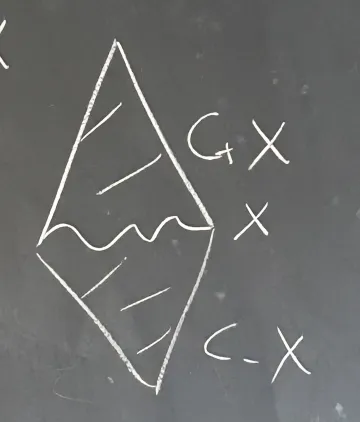
\includegraphics[width=0.3\textwidth]{Figures/pos_neg_cone.png}\]
    We can decompose the suspension map as the composition of the following maps:
% https://q.uiver.app/#q=WzAsNCxbMCwwLCJcXHBpX2koWCkiXSxbMSwwLCJcXHBpX3tpKzF9KENfKyBYLCBYKSJdLFsyLDAsIlxccGlfe2krMX0oU1gsIENfey19IFgpIl0sWzMsMCwiXFxwaV97aSsxfShYKSJdLFswLDEsIlxcY29uZyJdLFsxLDJdLFsyLDMsIlxcY29uZyJdXQ==
\[\begin{tikzcd}
	{\pi_i(X)} & {\pi_{i+1}(C_+ X, X)} & {\pi_{i+1}(SX, C_{-} X)} & {\pi_{i+1}(SX)}
	\arrow["\cong", from=1-1, to=1-2]
	\arrow[from=1-2, to=1-3]
	\arrow["\cong", from=1-3, to=1-4]
\end{tikzcd}\]
Here, the first isomorphism is induced by the LES of homotopy groups of the pair $(C_+ X, X)$. The second isomorphism is induced by the LES of homotopy groups of the pair $(SX, C_{-} X)$.\\

Let us now examine the map of pairs
\[(C_+ X, X) \to (SX, C_{-} X).\]
We know that $X$ itself is $(n-1)$-connected, this implies that, from the LES of homotopy groups, $(C_+ X, X)$ and $(C_{-} X, X)$ are both $n$-connected. In particular, this implies that, by the Homotopy Excision Theorem (Theorem~\ref{thm::homotopy_excision}), the induced map
\[\pi_{i+1}(C_{+} X, X) \to \pi_{i+1}(SX, C_{-} X)\]
is an isomorphism for $i+1 < 2n$ and a surjection for $i+1 = 2n$.
\end{proof}

Here is an application of the Freudethal Suspension theorem.
\begin{corollary}
    For all $n = 1, 2, ...$, we have that
    \[\pi_i(S^n) = \begin{cases}
        0, i < n\\
        \Zbb, i = n
    \end{cases}\]
    Furthermore, the isomorphism $\pi_n(S^n) \to \Zbb$ is implemented by the degree map.
\end{corollary}

\begin{proof}
We already know $\pi_i(S^n) = 0$ for $i < n$. For the second case, we have a sequence of maps induced by suspension
    % https://q.uiver.app/#q=WzAsNSxbMCwwLCJcXHBpXzEoU14xKSJdLFsxLDAsIlxccGlfMihTXjIpIl0sWzIsMCwiXFxwaV8zKFNeMykiXSxbMywwLCJcXHBpXzQoU140KSJdLFs0LDAsIi4uLiJdLFswLDEsImZfMSJdLFsxLDIsImZfMiJdLFszLDRdLFsyLDMsImZfMyJdXQ==
\[\begin{tikzcd}
	{\pi_1(S^1)} & {\pi_2(S^2)} & {\pi_3(S^3)} & {\pi_4(S^4)} & {...}
	\arrow["{f_1}", from=1-1, to=1-2]
	\arrow["{f_2}", from=1-2, to=1-3]
	\arrow["{f_3}", from=1-3, to=1-4]
	\arrow[from=1-4, to=1-5]
\end{tikzcd}\]
Now the Freudethal suspension theorem tells that $f_n$ is an isomorphism for $n < 2n - 1$ and a surjection for $n = 2n - 1$. So we know that $f_n$ is an isomorphism for $n = 2, 3, ...$ and $f_1$ is a surjection.\\

If we could show that $\pi_2(S^2) = \Zbb$, then we will show that each $\pi_n(S^n)$ is isomorphic to $\Zbb$. Now let us look at 
\[f_1: \pi_1(S^1) \to \pi_2(S^2).\]
We know $\pi_1(S^1) = \Zbb$ is generated by the identity map $1_{S^1}$. Now, we clearly have that $f_1(1_{S^1}) = 1_{S^2}$ (from the suspension functor). Since $f_1$ is a surjection, we know that $\pi_2(S^2)$ is actually generated by $1_{S^2}$. Thus, $\pi_2(S^2)$ is either a finite cyclic group or is $\Zbb$.\\

We know from a previous class (hopefully) that degree is homotopy invariant. We know that given $S^k$, there exists a basepoint-preserving map of degree $n$, given by essentially passing the map $S^k$ to $\bigvee_{i=1}^n S^k$, and map each copy of $S^k$ onto $S^k$ by identity. Here is a picture for $n = 4$
\[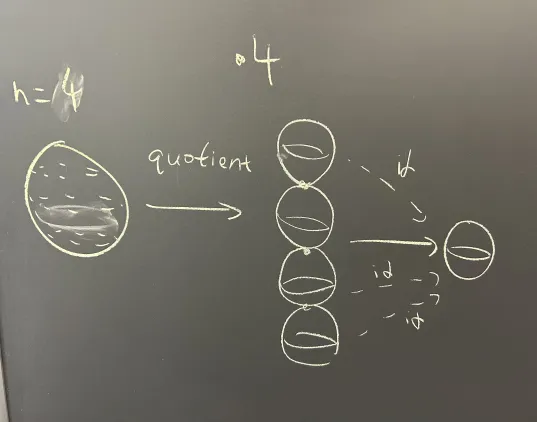
\includegraphics[width=0.5\textwidth]{Figures/degree_4_map.png}\]
For $k = 2$, this means that there is a map from $S^2$ to $S^2$ of degree $n$ for any $n$. Thus, $\pi_2(S^2)$ has to be infinite, and we thus conclude that $\pi_2(S^2) = \Zbb$.\\

Finally, to show that the degree map is an isomorphism. We know from the Freudenthal Suspension Theorem that $1_{S^2}$ generates $\pi_2(S^2)$, and following along the chain of isomorphisms and remembering that they are induced by suspension function, we have that each $1_{S^n}$ generates $\pi_n(S^n)$. If the degree map is a homomorphism, it certain sends generators to generators and is surjective (and injective), so it is an isomorphism.\\

Why is the dgree map a homomorphism? Well, for $\pi_1$, we know this from a previous class, hopefully. For $\pi_n$ in general, it follows from the standard fact that if $f: S^{n-1} \to S^{n-1}$ is a map and $Sf: S^{n} \to S^{n}$ is the induced map of the suspension functor, then $\deg f = \deg Sf$
\end{proof}

\begin{corollary}
    $\pi_n(\bigvee_{\alpha \in A} S^n) \cong \bigoplus_{\alpha \in A} \Zbb$, and $\pi_k(\bigvee_{\alpha \in A} S^n) = 0$ for $k < n$.
\end{corollary}

\begin{proof}
   Omitted. The same proof for a single sphere will work for this case.
\end{proof}

\begin{example}
    If $X$ is a finite CW complex, $H_{*}(X, \Zbb)$ is finitely generated because of cellular homology. The same thing, however, is not true for homotopy groups! Take $X = S^1 \vee S^2$ for example. The universal covering space $\Tilde{X}$ of $X$ is going to be the following diagram
    \[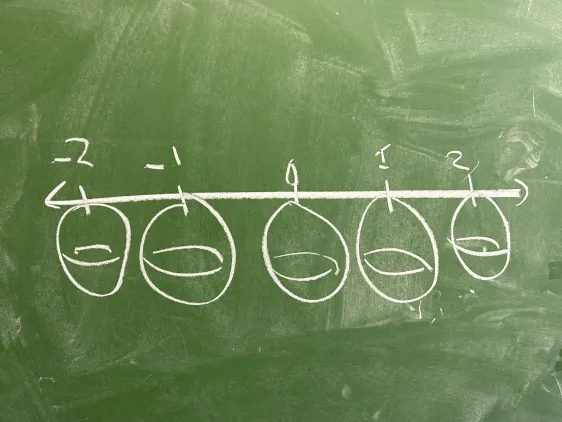
\includegraphics[width=0.5\textwidth]{Figures/s1_v_s2.png}\]
    So in particular, $\Tilde{X}$ is homotopy equivalent to $\bigvee_{n \in \Zbb} S^2$. In particular, 
    \[\pi_2(X) = \pi_2(\Tilde{X}) = \bigoplus_{n \in \Zbb} \Zbb \]
    is not finitely generated.
\end{example}

\begin{remark}
    There was a deviation away from the main lecture where we discussed whether the homotopy groups of a closed manifold is finitely generated. While we never reached a definite answer, it is always true that for a simply connected closed manifold, its homotopy groups are always finitely generated.\\
    
    We also noted that there are no closed manifolds that can be homotopy equivalent to $S^1 \vee S^2$. This is because the cup product structure $H^1(S^1 \vee S^2) \times H^1(S^1 \vee S^2) \to H^2(S^1 \vee S^2)$ is the zero map. If $M$ is a closed manifold homotopy equivalent to $S^1 \vee S^2$, then $\dim M = 2$ because $M$ is $\Zbb/2$-orientable, and the cup product map of $H^1(M) \times H^1(M) \to H^2(M)$ over $\Zbb/2$ has to be non-degenerate, by Poincare duality.
\end{remark}

\subsection{Eilenberg Maclane Space}

\begin{definition}
    $X$ is a $K(\pi, n)$ if $\pi_i(X) = \pi$ for $i = n$ and $0$ for $i \neq 0$. Here, $\pi$ is an abelian group if $n > 1$ and $\pi$ is a group if $n = 1$.
\end{definition}

\begin{theorem}
    Given any $\pi, n$ satisfying the definition above, there exists a CW-complex which is $K(\pi, n)$.
\end{theorem}

\begin{proof}
    We will only show this for $n > 1$. The case for $n = 1$, hopefully you have seen this in a previous class (according to the instructor). Every abelian group can be written as the surjection of a free abelian group. Let us write the surjection as
    \[\bigoplus_{\lambda \in \Lambda} \Zbb \to \pi \to 0.\]
    Let $R$ be the kernel of this surjection. Take $X_n = \bigvee_{\lambda \in \Lambda} S^n_{\lambda}$, then we have that
    \[\pi_i(X_n) = 0, i < n.\]
    \[\pi_n(X_n)  = \pi_n(\bigvee_{\lambda \in \Lambda} S^n_{\lambda}) = \bigoplus_{\lambda \in \Lambda} \Zbb.\]
    
    Looking at $R$, we know that $\bigoplus_{\lambda \in \Lambda} \Zbb \cong \pi_n(X_n)$, so we can take generators of $R$ and represent them by maps $\psi_r: S^n \to X_n$. Let $X_{n+1} = X_n \cup_{\psi} e^{n+1}$ again be the attachment of $X_n$ with each cell representing a generator in $R$ with the attaching map $\psi_r$.\\

    In this case, we claim that $\pi_n(X_{n+1}) = \pi$. From Corollary~\ref{cor::cw_skeleton_hom_gp}(c), we know that the inclusion map $i: X_n \to X_{n+1}$ induces a surjection on $i_*: \pi_n(X_n) \twoheadrightarrow \pi_n(X_{n+1})$. We claim that $\ker(i_*) = R$, so the first isomorphism theorem will conclude that $\pi_n(X_{n+1}) = \pi$. Indeed, recall $\psi_r: S^n \to X_n$ is a map whose representative is a generator of $X_n$, then $i \circ \psi_r: S^n \to X_{n+1}$ is going to be null-homotopic because the attachment of $e^{n+1}$ to $X_n$ by $\psi_r$ gives a very explicit homotopy from the boundary of $e^{n+1}$ to the center of $e^{n+1}$ (which we can think of all a constant map). Thus, we have that $R \subset \ker(i_*)$.\\
    
    On the other hand, suppose $f: S^n \to X_n$ is a map such that $i \circ f: S^n \to X_{n+1}$ is null-homotopic, we wish to show that $[f] \in R$. Since $i \circ f$ is based null-homotopic, let $H: S^n \times I \to X_{n+1}$ such that $H_0 = f$ and $H_1 = c_{x}$ with $x \in X_n$. If the image of $H$ is contained entirely in $X_n$, then $[f] = [0] \in \pi_n(X_n)$ and we are done. \mattie{After asking the instructor, the proof of $\pi_n(X_{n+1}) = \pi$ will be formally justified in the next lecture.}\\
    
    Now, we have shown that $\pi_n(X_{n+1}) = \pi$. Take generators $\psi_{\gamma}: S^{n+1} \to X^{n+1}$ for $\pi_{n+1}(X_{n+1})$ and attach them to create $X_{n+2} = X_{n+1} \cup_{\psi_\gamma} e^{n+2}$. This will kill $\pi_{n+1}(X_{n+2})$ and turn it into $0$. Indeed, if $f: S^{n+1} \to X_{n+2}$ is a based map, then by Cellular Approximation, $f$ without loss factors through $X_{n+1}$. We without loss write $f = i \circ \Tilde{f}$ where $i: X_{n+1} \to X_{n+2}$ is the inclusion map. The map $\Tilde{f}$ is given by generators $\psi_{\gamma}$'s. Thus, it suffices for us to check that each $i \circ \psi_{\gamma}$ represents $0$, which is exactly given by these cell attachments. Thus, we conclude that $\pi_{n+1}(X_{n+2}) = 0$.
    
    However, this does not affect $\pi_n$ and we have $\pi_{n}(X_{n+2}) = \pi$, because of the cellular approximation theorem. We can do this repeatedly going up and killing higher homotopy groups, which will give us the desired Eilenberg-Maclane space.
\end{proof}

\begin{remark}
    The proof that $\pi_n(X_{n+1}) = \pi$ is significantly simplified if the class has proven Hurewicz Theorem, but we have not proven Hurewicz Theorem. We observe that $X_{n+1}$ is $(n-1)$-connected, so Hurewicz Theorem implies that $\pi_n(X_{n+1})$ is isomorphic to $H_n(X_{n+1})$ by the Hurewicz map. The cellular homology of $H_n(X_{n+1})$ is significantly easier to compute, as $C_n(X_n, X_{n-1}) = C_n(X_n) = \bigoplus_{\lambda \in \Lambda} \Zbb$ and the cellular boundary formula tells us that the boundary map from $C_{n+1}(X_{n+1}, X_n) \to C_{n}(X_n, X_{n-1})$ has image exactly equal to $R$. 
\end{remark}

It is true that any two $K(\pi, n)$ which are CW-complexes are homotopy equivalent, we will prove this next lecture.

\newpage
\section{Lecture October 8th, 2024}

\textbf{Announcement: }We will not have classes for Thursday next week and Thursday next next week. For next Tuesday and next next Tuesday, we will be having double-block classes in algebraic topology to make up for them.

\subsection{Recall Materials from Last Time}

Let us recall the statement of excision for homotopy.
\begin{theorem}
    Suppose $X$ is a CW complex and $X = A \cup B$ is the union of two subcomplexes. Suppose $C = A \cap B$ is non-empty. If $(A, C)$ is $m$-connected and $(B, C)$ is $n$-connected, then the map induced by inclusion $\pi_i(A, C) \to \pi_i(X, B)$ is an isomorphism when $i < m+n$ and a surjection for $i = m+n$.
\end{theorem}

From here we obtained the following corollary.

\begin{corollary}
   We have that
   $$\pi_k(S^n) = \begin{cases}
       0, k < n\\
       \Zbb, k = n
   \end{cases},$$
   and the isomorphism $\pi_n(S^n) \to \Zbb$ can be given by the degree map. Furthermore, we have that
   \[\pi_n(\bigvee_{\alpha \in A} S^n_\alpha) = \bigoplus_{\alpha \in A} \Zbb. \]
   Here the inclusion $i_{\alpha}: S^n \to \bigvee_{a\in A} S^n_a$ given by sending $S^n$ onto the copy corresponding to $a$ represents the identity $1_{\alpha}$ in $\bigoplus_{a \in A} \Zbb$.
\end{corollary}

\begin{example}
    There are examples of closed manifolds whose $\pi_k$ is not finitely generated. Take $M = T^4 \# \Cbb P^2$ as the connected sum between the $4$-torus and $\Cbb P^2$. Since $\Cbb P^2$ itself is simply connected, the universal cover of $M$ is $\Rbb^4$ with every lattice point being wedged a copy of $\Cbb P^2$. In particular, each of the $\Cbb P^2$ has a generator in degree $2$ (by Hurewicz's theorem), so $\pi_2(M)$ is not finitely generated.
\end{example}

\subsection{Localizing Weak Homotopy Equivalences}
\begin{definition}
   We define an equivalence relation $X \sim Y$ if there exists a series of topological spaces $X_1 = X, X_2, ..., X_n = Y$ such that either for all $i$, there is a weak homotopy equivalence from $X_i \to X_{i+1}$ or from $X_{i+1} \to X_i$. We say that $X$ is weakly equivalent to $Y$ if $X \sim Y$ (note that there may not be a map from $X$ to $Y$ that is an isomorphism on all homotopy groups.)
\end{definition}

\begin{remark}
    In more categorical languages, we are secretly localizing all weak homotopy equivalences in the reasonable category of spaces we are working with. That being said, we are doing a naive brute-force version of localization that does not necessarily make a category. There is a more streamlined way of doing this using the idea of a homotopy categories.
\end{remark}

Here is a general ``rough" procedure for localizing a category.
\begin{definition}
    If $\mathcal{C}$ is a category and $S \subset \text{ class of morphisms}$, then we can create a localization category $C_{S}$, where for every morphism $s \in S$, it becomes an isomorphism in $C_{S}$. Thus, we are really just add a formal inverse $s^{-1}: Y \to X$ for every $s: X \to Y \in S$. For two objects $X, Y \in C_S$, the collection of morphisms
    \[C_S(X, Y)\]
    is a chain $X = X_1, X_2, ...., X_n = Y$ such that for each $i$, either there exists an element $s_i \in S$ from $X_i \to X_{i+1}$ or from $X_{i+1} \to X_i$.
\end{definition}

\begin{proposition}
    If $X$ is weakly equivalent to $Y$, then $H_*(X; A)$ is an isomorphism $H_*(X; A)$ with $A$ being any coefficient system, 
\end{proposition}

\begin{proof}
    Omitted, you may find a proof in Hatcher.
\end{proof}

\begin{remark}
    This constraint of weak equivalence is stronger than just having isomorphic homotopy groups. For example $S^2 \times \Rbb P^3$ and $\Rbb P^2 \times S^3$ have isomorphic homotopy groups, but their homology groups are not isomorphic.
\end{remark}

Here we obtain an analog of Excision for good pairs on homotopy groups.

\begin{proposition}\label{prop::quotient_exic}
    Let $(X, A)$ be a $r$-connected CW pair and $A$ itself is $s$-connected, then $\pi_k(X, A) \to \pi_k(X/A)$ is an isomorphism for $k\leq r+s$ and a surjection for $k = r+s+1$.
\end{proposition}

\begin{proof}
    Let $X \cup CA$ be the cofiber of the inclusion map $i: A \to X$. In this case, $CA$ is contractible and is a subcomplex of $X \cup CA$. Furthermore, $X \cup CA/CA$ is clearly homeomorphic to $X/A$. Now we can consider the map
    \[X \cup CA \to X \cup CA/CA \cong X/A.\]
    From here we can consider the diagram
% https://q.uiver.app/#q=WzAsNSxbMCwwLCJcXHBpX2koWCwgQSkiXSxbMSwwLCJcXHBpX2koWCBcXGN1cCBDQSwgQ0EpIl0sWzIsMCwiXFxwaV9pKFggXFxjdXAgQ0EvQ0EpIl0sWzMsMCwiXFxwaV9pKFgvQSkiXSxbMiwxLCJcXHBpX2koWCBcXGN1cCBDQSkiXSxbMiwzLCJcXGNvbmciXSxbMCwxLCIoMikiXSxbMSwyXSxbNCwyLCIoMSkiXSxbNCwzLCJcXGNvbmciLDJdXQ==
\[\begin{tikzcd}
	{\pi_i(X, A)} & {\pi_i(X \cup CA, CA)} & {\pi_i(X \cup CA/CA)} & {\pi_i(X/A)} \\
	&& {\pi_i(X \cup CA)}
	\arrow["{(2)}", from=1-1, to=1-2]
	\arrow[from=1-2, to=1-3]
	\arrow["\cong", from=1-3, to=1-4]
	\arrow["{(1)}", from=2-3, to=1-3]
	\arrow["\cong"', from=2-3, to=1-4]
\end{tikzcd}\]
    Here $(1)$ is an isomorphism by the quotient map $X \cup CA \to X \cup CA/CA$ (this is because $CA$ is contractible and $(X \cup CA, CA)$ is a CW pair, so modding out $CA$ is a homotopy equivalence). (2) is induced by inclusion $(X, A) \to (X \cup CA, CA)$, we can apply the homotopy excision theorem to this map and get that:
    \begin{enumerate}
        \item $\pi_i(X, A) \to \pi_i(X \cup CA, CA)$ is an isomorphism for $i \leq r + s$.
        \item $\pi_i(X, A_ \to \pi_i(X \cup CA, CA)$ is srujective for $i = r+s+1$.
        \item This is because $(CA, A)$ is $(s+1)$-connected.
    \end{enumerate}
\end{proof}

\subsection{Eilenberg Maclane Spaces - Part Two}
Now we return back to the theorem from last time, which the note-taker pointed out an error from last time. That is why we are fixing it.
\begin{proposition}
    For any $n \geq 1$, $A$ a group (abelian if $n > 1$), then there exists a CW complex $X$ that is $K(A, n)$.
\end{proposition}

\begin{proof}
    We only show that for $n > 1$. Let $A$ be an abelian group, then $A$ is srujected onto by a free-abelian group
    \[\bigoplus_{a \in \mathcal{A}} \Zbb \to A \to 0.\]
    Let $X^n = \bigvee_{a \in \mathcal{A}} S^n_a$, then we know that
    \[\pi_k(X^n) \cong \begin{cases}
        0, k < n\\
        \bigoplus_{a \in \mathcal{A}} \Zbb, k = n
    \end{cases}.\]
    Since $\pi_n(X^n) = \bigoplus_{a \in \mathcal{A}} \Zbb$, we have a surjection
    \[\pi_n(X^n) \to A \to 0.\]
    Let $R$ be the kernel of this surjection $\pi_n(X^n) \to A$. We take $\beta \in B$ as a set of generators for $R$, and represent each $\beta$ by a map $\varphi_\beta: S^n \to X^n$. We attach an $(n+1)$-cell to $X^n$ by $\varphi_\beta$ for each $\beta$, ie.
    \[X^{n+1} = X^n \cup \bigcup_{\beta} e_{\beta}^{n+1}.\]
    Using cellular approximation, we know that $\pi_k(X^{n+1}) = 0$ for $k < n$.\\

    For $k = n$, we consider the long exact sequence of the pairs $(X^{n+1}, X^n)$. Here we have that
    % https://q.uiver.app/#q=WzAsNCxbMCwwLCJcXHBpX3tuKzF9KFhee24rMX0sIFhebikiXSxbMSwwLCJcXHBpX24oWF5uKSJdLFsyLDAsIlxccGlfbihYXntuKzF9KSJdLFszLDAsIjAiXSxbMCwxXSxbMSwyXSxbMiwzXV0=
\[\begin{tikzcd}
	{\pi_{n+1}(X^{n+1}, X^n)} & {\pi_n(X^n)} & {\pi_n(X^{n+1})} & 0
	\arrow[from=1-1, to=1-2]
	\arrow[from=1-2, to=1-3]
	\arrow[from=1-3, to=1-4]
\end{tikzcd}\]
Thus, by Proposition~\ref{prop::quotient_exic}, we have that 
\[\pi_i(X^{n+1}, X^n) \to_f \pi_i(X^{n+1}/ X^n) = \pi_i(\bigvee_{\beta \in B} S_{\beta}^{n+1}).\]
is an isomorphism for $i \leq 2n-1$, and a surjection for $i = 2n$. In particular since $n > 1$, we have that
\[\pi_{n+1}(X^{n+1}, X^n) \cong \pi_{n+1}(X^{n+1}/X^n) = \bigoplus_{\beta \in B} \Zbb.\]
THe map $f$ behaves exactly how one might expect. For the class given by $i_{\beta}: S^{n+1} \to \bigoplus_{\beta \in B} S^{n+1}_{\beta}$, we send it to $[\varphi_{\beta}] \in \pi_n(X^n)$. Thus, $\operatorname{im}(f)$ is exactly the subgroup generated by $[\varphi_{\beta}]$, so $\operatorname{im}(f) = R$. This implies that $\pi_n(X^{n+1}) \cong A$ from the long exact sequence.\\

Now, we have that
\[\pi_k(X^{n+1}) = \begin{cases}
    0, k < n\\
    A, k = n
\end{cases}.\]
We wish to kill $\pi_{n+1}(X^{n+1})$. Take generators $\psi_{\gamma}: S^{n+1} \to X^{n+1}$ for $\pi_{n+1}(X_{n+1})$ and attach them to create $X_{n+2} = X_{n+1} \cup_{\psi_\gamma} e^{n+2}$. This will kill $\pi_{n+1}(X_{n+2})$ and turn it into $0$. Indeed, if $f: S^{n+1} \to X_{n+2}$ is a based map, then by Cellular Approximation, $f$ without loss factors through $X_{n+1}$. We without loss write $f = i \circ \Tilde{f}$ where $i: X_{n+1} \to X_{n+2}$ is the inclusion map. The map $\Tilde{f}$ is given by generators $\psi_{\gamma}$'s. Thus, it suffices for us to check that each $i \circ \psi_{\gamma}$ represents $0$, which is exactly given by these cell attachments. Thus, we conclude that $\pi_{n+1}(X_{n+2}) = 0$.\\
    
However, this does not affect $\pi_n$ and we have $\pi_{n}(X_{n+2}) = \pi$, because of the cellular approximation theorem. We can do this repeatedly going up and killing higher homotopy groups, which will give us the desired Eilenberg-Maclane space.
\end{proof}

From the proof of constructing Eilenberg Maclane spaces, we can similarly see a proof of the following.
\begin{proposition}
    Suppose $X = (\bigvee_{a \in A} S^n_{\alpha}) \cup \bigcup_{\beta \in B} e^{n+1}_\beta$. Then for any path-connected space $Y$ and any homomorphism
    \[\psi: \pi_n(X) \to \pi_n(Y),\]
    there exists $f: X \to Y$ such that $\psi = f_*$.
\end{proposition}

\begin{proof}
    Send the basepoint of $X_n = \bigvee_{a \in A} S^n_{\alpha}$ to $y_0 \in Y$. From here, we define $f_n: X^n \to Y$ to be given by: for any $i_\alpha: S^n \to \bigvee_{\alpha \in A} S^n_{\alpha}$, we send $f_n([i_{\alpha}])$ to a map representing $\psi([i \circ i_{\alpha}]) \in \pi_n(Y)$ (here $i$ is the inclusion of $X^n$ to $X$).\\

    This defines a map $f_n: X^n \to Y$ such that $(f_n)_*: \pi_n(X^n) \to \pi_n(Y)$ satisfies the following
    \[(f_n)_*([i_{\gamma}]) = \psi([i \circ i_{\gamma}]).\]
    Since the $[i_{\gamma}]$'s generate $\pi_n(X^n)$, this implies that
    \[(f_n)_*(\varphi) = \psi([i \circ \varphi]), \text{ for all } \varphi \in \pi_n(X).\]
    Now, we wish to extend $f_n$ to $f_{n+1}: X^{n+1} \to Y$. We observe that $\varphi_{\beta}$ is null-homotopic in $X^{n+1}$ because of the attaching maps. Thus, $f \circ \varphi_{\beta}$ is null-homotopic in $Y$. (Recall a nullhomotopic map extends to a continuous map on the disk), thus $f_n$ extends over each disks attached onto a continuous map $f_{n+1}: X^{n+1} \to Y$.\\

    Why does $f_{n+1}$ induce the exact same map as $\psi$? We first observe that we do have the commutative diagram
    % https://q.uiver.app/#q=WzAsMyxbMCwwLCJcXHBpX24oWF5uKSJdLFsyLDAsIlxccGlfbihYXntuKzF9KSJdLFsxLDEsIlxccGlfbihZKSJdLFswLDEsImlfKiIsMCx7InN0eWxlIjp7ImhlYWQiOnsibmFtZSI6ImVwaSJ9fX1dLFswLDIsIihmX24pXyoiLDJdLFsxLDIsIihmX3tuKzF9KV8qIl1d
\[\begin{tikzcd}
	{\pi_n(X^n)} && {\pi_n(X^{n+1})} \\
	& {\pi_n(Y)}
	\arrow["{i_*}", two heads, from=1-1, to=1-3]
	\arrow["{(f_n)_*}"', from=1-1, to=2-2]
	\arrow["{(f_{n+1})_*}", from=1-3, to=2-2]
\end{tikzcd}\]
%From the same proof in the construction of the Eilenberg Maclane space, we can see that $i_*: \pi_n(X^n) \to \pi_n(X^{n+1})$ is a surjection with the kernel being generated exactly by $[\varphi_\beta: S^n \to X^n]$ in $\pi_n(X^n)$ for all $\beta \in B$.\\

Let us now check that $(f_{n+1})_* = \psi$. Indeed, for any $g: S^n \to X^{n+1}$, by cellular approximation without loss $g$ factors through $i \circ g'$ for some $g': S^n \to X^n$. Thus, we have that
\[(f_{n+1})_*([g]) = [f_{n+1} \circ i \circ g'] = [f_n \circ g'] = (f_n)_*([g']) = \psi([i \circ g']) = \psi([g]).\]

\end{proof}

\begin{corollary}
    If $X = K(A, n)$ is a CW-complex, then $X$ is unique up to homotopy equivalence.
\end{corollary}

\begin{proof}
    If $X$ and $X'$ are two CW $K(A, n)$. We can assume through the construction that we have of $K(A, n)$'s that $X = \bigvee_{a \in A} S^{n}_a \cup \bigcup_{b \in B} e_b^{n+1} \cup (\text{higher cells})$. From here, we see that 
    \[X^{n+1} = \bigvee_{a \in A} S^{n}_a \cup \bigcup_{b \in B} e_b^{n+1}. \]
    From the previous prposition, we know there exists a map $f_{n+1}: X^{n+1} \to X'$ that gives an isomorphism on $\pi_n$. Now we can extend $f_{n+1}$ onto $e^{n+2}_\gamma$, we just need that $f_{n+1} \circ \varphi_{\gamma}$ is null-homotopic, but it is since $\pi_{n+1}(X') = 0$. Thus, we can do this simultaneously and also get a map $f_{n+2}: X^{n+2} \to X'$ and adding $n+2$ cells does not affect the map $f_{n+2}$ on $\pi_n$.\\

    Thus, we can keep doing this going up to produce a desired weak homotopy equivalence. By Whitehead's Theorem, this gives a homotopy equivalence. 
\end{proof}

\subsection{Hurewicz Theorem}

\begin{definition}
    Let $X$ be a space, there is a Hurewicz map
    \[h_k: \pi_k(X) \to \Tilde{H}_k(X),\]
    where given $\phi: S^k \to X$, and $[S^k] \in H_k(S^k)$ be its fundamental class.
    \[[\phi] \mapsto \phi_*([S^k]) \in \Tilde{H}_k(X).\]
\end{definition}

\begin{theorem}[Hurewicz Theorem]
    Let $n \geq 2$. If $X$ is $(n-1)$-connected  then $h_k$ is an isomorphism for $k \leq n$. In particular, this implies that $\Tilde{H}_k(X) = 0$ for $k \leq n-1$ and $\Tilde{H}_n(X) \cong \pi_n(X)$.\\
    
    Moreover, there is a relative version of the statement where if $(X, A)$ is $(n-1)$-connected and $A$ is simply connected, then $H_i(X, A) = 0$ for $i \leq n-1$ and $\pi_n(X, A) \cong H_n(X, A)$.
\end{theorem}

\begin{remark}
    There is a Hurewicz theorem for $n = 1$ that states $\Tilde{H}_1(X)$ is the abelianization of $\pi_1(X)$.
\end{remark}

\newpage
\section{Lecture October 10th, 2024}

\subsection{Hurewicz Theorem - Continued}

\begin{theorem}[Hurewicz Theorem]
    If $X$ is $(n-1)$-connected for $n \geq 2$, then the reduced homology $\Tilde{H}(X) = 0$ for $i \leq n - 1$, and the Hurewicz homomorphism
    \[h_n: \pi_n(X) \to H_n(X)\]
    is an isomorphism. Here $h_n$ is defined by
    \[h_n(\varphi: S^n \to X) = \varphi_*([S^n]) \in H_n(X).\]
    Note that a concrete way to interpret the Hurewicz map $h_n$ is as follows - there is a canonical map $q$ from an $n$-simplex $\Delta^n$ to $S^n$ by quotienting its boundary. Thus $\varphi \circ q: \Delta^n \to X$ is a singular $n$-simplex and we send
    \[[\varphi] \mapsto [\varphi \circ q].\]
    Moreover, if the pair $(X, A)$ is $(n-1)$-connected and $A$ is simply connected, then 
    \[H_{i}(X, A) = 0 \text{ for $i \leq n - 1$ and } h_n: \pi_n(X, A) \to H_n(X, A)\]
    is an isomorphism. Here, $h_n$ is defined similarly as before.
\end{theorem}

\begin{proof}
    We will not prove why the Hurewicz map is an isomorphism here, but we will prove everything else. Without loss of generality by the CW approximation theorem, we may assume that $(X, A)$ is a CW-pair. We observe that the relative case follows from the absolute case, because when $(X, A)$ is a CW pair, we know we can identify by the Homotopy Excision Theorem
    \[\pi_i(X, A) \cong \pi_i(X/A), i \leq n.\]
    Since $(X, A)$ is a good pair, we also have that
    \[H_{k}(X, A) \cong \Tilde{H}_k(X/A).\]
    Thus, it suffices for us to prove this in the absolute case when $X$ is a CW complex. By the CW approximation theorem and since $X$ is $(n-1)$-connected, we can furthermore assume without loss that $X^{n-1}$ is a point.\\

    We note that $\Tilde{H}_k(X) = 0$ for $k < n-1$ by cellular homology (there is only $1$ cell below dimension $n$, which is a point). Now we want to check that $\pi_n(X) \cong H_n(X)$. To do this, we can without loss replace $X$ by its $(n+1)$-skeleton (this does not affect the $k$-th homotopy group/homology for $k \leq n$), so we without loss have that
    \[X = \bigvee_{a \in A} S^n_{\alpha} \cup \bigcup_{b \in B} e_b^{n+1}.\]
    From the LES of the pair $(X^{n+1}, X^n)$, we have that
    \[\pi_{n+1}(X^{n+1}, X^n) \to \pi_n(X^n) \to \pi_n(X^{n+1}) \to \pi_{n}(X^{n+1}, X^n) \to ...\]
    We know that $\pi_{n}(X^{n+1}, X^n) = 0$, so exactness implies that $\pi_{n}(X^{n+1})$ is the cokernel of the map
    \[\bigoplus_{b \in B} \Zbb = \pi_{n+1}(X^{n+1}, X^n) \to_{\partial_\pi} \pi_n(X^n) = \bigoplus_{a \in A} \Zbb\]

    \textbf{Claim:} This map $\partial_\pi$ coincides with the map in the construction of the cellular homology
    \[\partial: H_{n+1}(X^{n+1}, X^n) \to H_n(X^n, X^{n-1}) = H_n(X^n, \star).\]
    From last semester at UPenn, we learned that cellular homology says that - for the free generators $e^{n+1}_\beta \in H_{n+1}(X^{n+1}, X^n)$, the coefficients of $\partial(e^{n+1}_\beta)$ are the degrees of the map
    \[S^n \to_{\varphi_\beta} X = \bigvee_{a \in A} S^n_{\alpha} \to_q S^n_{\alpha}. \]
    Here $\varphi_\beta$ is the restriction of the characteristic map of $e^{n+1}_\beta$ to boundary, onto $X^n$ in the construction of $X^{n+1}$ and $q$ is the quotient map of $\bigvee_{a \in A} S^n_{\alpha}$ that collapses all other copies of $S^n$ to the basepoint except for $S^n_{\alpha}$.\\

    However, this coefficient is the same as the one given by $\partial_{\pi}$ because the isomorphism $\pi_n(S^n) \to \Zbb$ is given by the degree map.
\end{proof}

\begin{remark}
    We will see another proof of this when we get to spectral sequences, where we will also prove that the Hurewicz map is an isomorphism.
\end{remark}

From here we obtain a corollary that is sometimes also called Whitehead's theorem.
\begin{corollary}
Let $f: X \to Y$ be a map between simply-connected CW complexes, and $f_*: H_k(X) \to H_k(Y)$ is an isomorphism for all $k$, then $f$ is a homotopy equivalence.
 \end{corollary}

\begin{proof}
    From cellular approximation, we can without loss assume $f$ is a cellular map. We can also replace $Y$ by the mapping cylinder of $f$ (which is CW since $f$ is cellular) since it is homotopy equivalent to $Y$. We can assume then that $X$ is a subcomplex of $Y$. Since $X$ is now a subcomplex of $Y$, we can use the LES of relative homology $(Y, X)$ and we see that
    \[H_k(Y, X) = 0 \text{ for all $k$}.\]
    Now since $\pi_1(X) = \pi_1(Y) = 0$, and since $H_1$ is the abelianization of $\pi_1$ (this is sometimes also called Hurewicz's theorem), we know that
    \[H_1(X) = H_1(Y) = 0.\]
    Now since $H_1(Y, X) = H_2(Y, X) = 0$ and $X$ is simply-connected, Hurewicz's theorem implies that $\pi_2(Y, X) = 0$. You could go up from this and similarly show that each $\pi_n(Y, X) = 0$ for all $n$. Hence, from the LES of homotopy groups for the pair $(Y, X)$, $f$ induces an isomorphism between their homotopy groups. Thus, the original whitehead implies that $f$ is a homotopy equivalence.
\end{proof}

\begin{example}
    Here are some applications of the Hurewicz Theorem and its corollaries.
    \begin{itemize}
        \item 0) Since $S^n$ is $(n-1)$-connected, we have another proof that $\pi_k(S^n) \cong H_n(S^n)$ for $k \leq n$.
        \item 1) Suppose $X$ is a closed simply-connected $3$-manifold, then $X$ is homotopy equivalent to $S^3$. To see this, we note that $\pi_1(X) = 0$ implies that $H_1(X) = 0$. Since $\pi_1(X) = 0$, $X$ itself is orientable (this is because its oriental double cover is two copies of $X$). Thus, this implies that $H_3(X) = \Zbb$. Now since $H^1(X) = 0$ from the Universal Coefficient Theorem, Poincare duality implies that $H_2(X) = 0$.\\

        Since $\pi_1(X) = 0$, Hurewicz's Theorem implies that $\pi_2(X) \cong H_2(X) = 0$. Thus $X$ is $2$-connected, and by Hurewicz's theorem, this implies that $\pi_3(X) = \Zbb$. Now let $f: S^3 \to X$ be a map representing the generator of $\pi_3(X)$, we can apply Whitehead's theorem to see that $f_*: H_k(S^3) \to H_k(X)$ is an isomorphism for all $k$.
    \end{itemize}
\end{example}

\subsection{Quillen's Plus Construction}
Here is another application.

\begin{definition}
    A group $G$ is called perfect if $G = [G, G]$ (it equals to its own commutative subgroup).
\end{definition}

\begin{theorem}
    Suppose $X$ is a CW complex with $H_1(X) = 0$ (ie. this is equivalent to $\pi_1(X)$ being perfect), then there exists $i: X \to X^+$ where $X^+$ is obtained from $X$ by attaching 2-cells and 3-cells such that $X^+$ is simply-connected and $i_*: H_k(X) \to H_k(X^+)$ is an isomorphism for all $k$.
\end{theorem}

\begin{proof}
    Let $\varphi_\alpha: S^1 \to X$ be the loops corresponding to generators of $\pi_1(X)$. Let $X' = X \cup \bigcup_{\alpha \in A} e^2_\alpha$ with attachment maps given by $\varphi_\alpha$. THis kills $\pi_1$ and we thus have that
    \[\pi_1(X') = 0.\]
    From the LES of relative homology on $(X', X)$, we have that
% https://q.uiver.app/#q=WzAsMTMsWzAsMCwiSF97aysxfShYJywgWCkgPSAwIl0sWzEsMCwiSF9rKFgpIl0sWzMsMCwiSF97a30oWCcsIFgpID0gMCJdLFsyLDAsIkhfayhYJykiXSxbMSwyLCJIXzIoWCkiXSxbMiwyLCJIXzIoWCcpIl0sWzMsMiwiSF8yKFgnLCBYKSA9IDAiXSxbMSwzLCJIXzEoWCkgPSAwIl0sWzIsMywiSF8xKFgnKSA9IDAiXSxbMywzLCJIXzEoWCcsIFgpIl0sWzEsMSwiLi4uIl0sWzQsMCwiayBcXGdlcSAzIl0sWzQsMywiLi4uIl0sWzAsMV0sWzEsM10sWzMsMl0sWzIsMTBdLFsxMCw0XSxbNCw1XSxbNSw2XSxbNiw3XSxbNyw4XSxbOCw5XSxbOSwxMl1d
\[\begin{tikzcd}
	{H_{k+1}(X', X) = 0} & {H_k(X)} & {H_k(X')} & {H_{k}(X', X) = 0} & {k \geq 3} \\
	& {...} \\
	& {H_2(X)} & {H_2(X')} & {H_2(X', X)} \\
	& {H_1(X) = 0} & {H_1(X') = 0} & {H_1(X', X)} & {...}
	\arrow[from=1-1, to=1-2]
	\arrow[from=1-2, to=1-3]
	\arrow[from=1-3, to=1-4]
	\arrow[from=1-4, to=2-2]
	\arrow[from=2-2, to=3-2]
	\arrow[from=3-2, to=3-3]
	\arrow[from=3-3, to=3-4]
	\arrow[from=3-4, to=4-2]
	\arrow[from=4-2, to=4-3]
	\arrow[from=4-3, to=4-4]
	\arrow[from=4-4, to=4-5]
\end{tikzcd}\]
In particular, we have that $H_k(X) \cong H_{k}(X')$ for $k \geq 2$, and we have the short exact sequence
\[0 \to H_2(X) \to H_2(X') \to H_2(X', X) \to 0\]
Now $H_2(X', X)$ is a free abeoian group $\bigoplus_{a \in A} \Zbb$. Thus, since free modules are projective, this sequence splits and we have that
\[H_2(X') \cong H_2(X) \oplus H_2(X', X).\]
Now, since $\pi_1(X') = 0$, we know that $\pi_2(X') \cong H_2(X')$ from Hurewicz's theorem.\\

We can represent a basis for $H_2(X', X) \subseteq H_2(X)$ by $\psi_{\beta}: S^2 \to X'$. WLOG, we can assume each $\psi_{\beta}$ are cellular maps, and we attach the $3$-cells to $X'$ by $\psi_{\beta}$ and form
\[X^+ \coloneqq X' \cup \bigcup_{b \in B} e^3_\beta.\]
In this case, $\pi_1(X^+)$ is still $0$ (adding $3$-cells does not change homotopy group). Furthermore, $H_k(X^+, X) = 0$ by the construction (for $k \neq 2$ it comes from the LES, for $k=2$ it comes from this construction). 
\end{proof}

The theorem is a special case of Quillen's Plus Construction.

\begin{theorem}
    Let $X$ be a CW complex. Let $H \subseteq \pi_1(X)$ be perfect. There exists $X^+$ and a map $f: X \to X^+$ which induces an isomorphism on homology and $\pi_1(X^+) \cong \pi_1(X)/N(H)$. Here, $N(H)$ denotes the normal closure of $H$ in $\pi_1(X)$. 
\end{theorem}

\begin{proof}
    Since $H$ is a subgroup of $\pi_1(X)$, we consider a covering space $p: X_H \to X$ that corresponds to the subgroup $H$. In this case, $\pi_1(X_H) = H$, which by hypothesis is perfect. From the previous theorem, we can form a plus construction $(X_H^)+$ to find a map
    \[i_H: X_H \to (X_H)^+\]
    that is an isomorphism on homology and $(X_H)^+$ itself is simply-connected. Now, we form the mapping cylinder $\operatorname{Cyl}(p)$ of the covering map $p$. Thus, we define $X^+$ to be the pushout of $i_H$ and the canonical inclusion $X_H \to \operatorname{Cyl}(p)$. Thus, we have
    % https://q.uiver.app/#q=WzAsNSxbMSwwLCJYX0giXSxbMiwwLCIoWF9IKV4rIl0sWzEsMSwiXFxvcGVyYXRvcm5hbWV7Q3lsfShwKSJdLFswLDEsIlgiXSxbMiwxLCJYXisiXSxbMCwxLCJpX0giXSxbMiwzLCJcXHNpbWVxIl0sWzAsMl0sWzIsNF0sWzEsNF1d
\[\begin{tikzcd}
	& {X_H} & {(X_H)^+} \\
	X & {\operatorname{Cyl}(p)} & {X^+}
	\arrow["{i_H}", from=1-2, to=1-3]
	\arrow[from=1-2, to=2-2]
	\arrow[from=1-3, to=2-3]
	\arrow["\simeq", from=2-2, to=2-1]
	\arrow[from=2-2, to=2-3]
\end{tikzcd}\]
Concretely, $X^+ = \operatorname{Cyl}(p) \cup_{X_H} X^+_H$. Now, by Van Kampen's Theorem (which is a statement of pushout), we know that there is a surjection
\[\pi_1(X) \to \pi_1(X^+) \to 0\]
with kernel being the normal closure of $H$.\\

Furthermore, we have that
\[X^+/\operatorname{Cyl}(p) = X^+_H/X_H.\]
Since the induced map $H_*(X_H) \to H_*(X_H^+)$ is an isomorphism. From the Long Exact Sequence, we know that
\[0 = H_*(X^+_H, X_H) = H_*(X^+_H/X_H) \cong H_*(X^+/\operatorname{Cyl}(p)).\]
Thus, $H_*(\operatorname{Cyl}(p)) \cong H_*(X) \to H_*(X^+)$ is an isomorphism for all $*$ by the LES of relative homology.
\end{proof}

\begin{remark}
    Quillen's $+$ construction was used to solve Adam's problem, which was concerned with Adams map in $K$-theory.
\end{remark}

Let $\Sigma_{\infty}$ be the permutations of $\Nbb$ (note that we can take $\Sigma_{\infty} = \bigcup \Sigma_n$ as the increasing union of the finite permutation groups). Now, from here we can form an index $2$ subgroup called $A_{\infty}$ that is perfect.\\

Consider the Eilenberg-Maclane space $K(\Sigma_{\infty}, 1)$ and let $X^+ = K(\Sigma_{\infty}, 1)^+$ be the plus construction with respect to $A_{\infty}$.

\begin{theorem}
    $\pi_i(X^+) \cong \pi_i^s$, where $\pi_i^s$ are the stable homotopy groups of spheres.
\end{theorem}

Since we haven't defined what a stable homotopy groups of spheres is in this class, we better define it.
\begin{definition}
    From the Freudenthal Suspension theorem, this chain of maps given by the Suspension functor eventually stabilizes to a chain of isomorphisms
    \[\pi_{i}(S^0) \to \pi_{i+1}(S^{1}) \to \pi_{i+2}(S^{2}) \to ...\]
    We define the stable homotopy group $\pi_i^s$ as
    \[\pi_i^s = \lim_{k \to \infty} \pi_{i+k}(S^k).\]
\end{definition}

\begin{example}
    $\pi_0 \Sbb = \Zbb \{1\}$ and $\pi_1 \Sbb = \Zbb/2 \{\eta\}$, where $\eta$ is the generator of $\pi_1 \Sbb$ and is the Hopf map $S^3 \to S^2$.
\end{example}

Here is another construction. Let $R$ be a ring, and we can form $GL_{\infty}(R) = \bigcup_{n=1}^\infty GL_n(R)$. It turns out that the commutator subgroup of $GL_{\infty}(R)$ is perfect.

\begin{definition}[Quillen's Definition of Algebraic $K$-theory]
    We define
    \[K_i(R) \coloneqq \pi_i(K(GL_{\infty}(R), 1)^+), i \geq 1.\]
    There is of course a $K_0(R)$, which is defined separately.
\end{definition}

\newpage
\section{Lecture October 15th, 2024 - Morning}

\subsection{Serre Fibrations}
Recall that a map $p: Y \to X$ is a \textbf{fibration} if it satisfies the homotopy lifting property for all spaces $Z$, $f: Z \to Y$ and homotopy $H: Z \times I \to X$, we admit a lift $\Tilde{H}: Z \times I \to Y$ such that 
% https://q.uiver.app/#q=WzAsNCxbMSwwLCJZIl0sWzEsMSwiWCJdLFswLDAsIlogXFx0aW1lcyBcXHswXFx9Il0sWzAsMSwiWiBcXHRpbWVzIEkiXSxbMCwxLCJwIl0sWzIsM10sWzMsMSwiSCIsMl0sWzIsMCwiZiJdLFszLDAsIlxcVGlsZGV7SH0iLDAseyJzdHlsZSI6eyJib2R5Ijp7Im5hbWUiOiJkYXNoZWQifX19XV0=
\[\begin{tikzcd}
	{Z \times \{0\}} & Y \\
	{Z \times I} & X
	\arrow["f", from=1-1, to=1-2]
	\arrow[from=1-1, to=2-1]
	\arrow["p", from=1-2, to=2-2]
	\arrow["{\Tilde{H}}", dashed, from=2-1, to=1-2]
	\arrow["H"', from=2-1, to=2-2]
\end{tikzcd}\]
commutes.\\

\begin{definition}
    A fibration is also called a \textbf{Hurewicz fibration}. There is, however, a more general notion of fibration - we say $p: Y \to X$ is a \textbf{Serre fibration} if it has the HLP with respect to all CW complexes. 
\end{definition}

\begin{remark}
    Usually in homotopy theory, when people say the word ``fibration" - they usually mean ``Serre fibration".
\end{remark}

\begin{definition}
    We say that $p: Y \to X$ has a HLP with respect to a pair $(A, B)$ if this exists and commutes
    % https://q.uiver.app/#q=WzAsNCxbMCwxLCJBIFxcdGltZXMgSSJdLFswLDAsIkEgXFx0aW1lcyBcXHswXFx9IFxcY3VwIChCIFxcdGltZXMgSSkiXSxbMSwwLCJZIl0sWzEsMSwiWCJdLFsxLDAsIiIsMCx7InN0eWxlIjp7InRhaWwiOnsibmFtZSI6Imhvb2siLCJzaWRlIjoidG9wIn19fV0sWzIsMywicCJdLFswLDMsIkgiLDJdLFsxLDIsImYiXSxbMCwyLCJcXFRpbGRle0h9IiwwLHsic3R5bGUiOnsiYm9keSI6eyJuYW1lIjoiZGFzaGVkIn19fV1d
\[\begin{tikzcd}
	{A \times \{0\} \cup (B \times I)} & Y \\
	{A \times I} & X
	\arrow["f", from=1-1, to=1-2]
	\arrow[hook, from=1-1, to=2-1]
	\arrow["p", from=1-2, to=2-2]
	\arrow["{\Tilde{H}}", dashed, from=2-1, to=1-2]
	\arrow["H"', from=2-1, to=2-2]
\end{tikzcd}\]
\end{definition}

\begin{proposition}
The following are equivalent:
\begin{enumerate}
    \item $p: Y \to X$ is a Serre fibration.
    \item $p$ satisfies the HLP relative to $D^k$ (closed disks).
    \item $p$ satisfies the HLP relative to the pair $(D^k, \partial D^k)$.
    \item $p$ satisfies the HLP relative to the pair $(Z, B)$
\end{enumerate}
\end{proposition}

\begin{proof}
    The equivalence between the second and third item is best explained by examining the following picture. Consider the pair $(D^k \times I, D^{k} \times \{0\})$ and $(D^k, \partial D^k)$:
    \[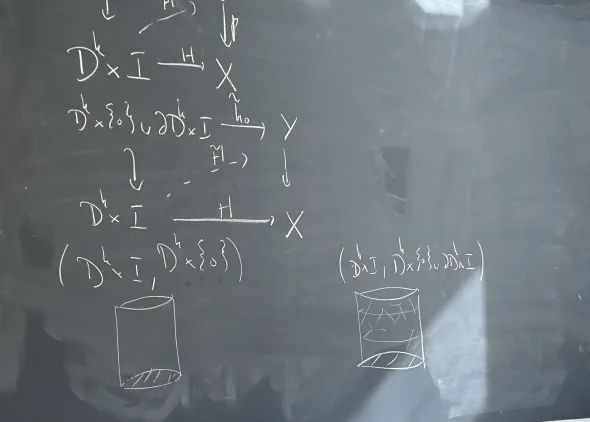
\includegraphics[width=0.35\textwidth]{Figures/soup_can_again.png}\]
    These two pairs are clearly homeomorphic as pairs (consider the soup can analogy laid out in Lemma~\ref{lem::relative_pin_null}), and thus $p: Y \to X$ has HLP to one if and only if has HLP to the other.

    Clearly (1) implies (2), which implies (3). To show that (3) implies (4), we observe that for any CW pair $(Z, B)$, we consider the following, which one can show has a lift due to universal properties
    % https://q.uiver.app/#q=WzAsNCxbMCwwLCJaIFxcdGltZXMgXFx7MFxcfSBcXGN1cCBCIFxcdGltZXMgSSJdLFsxLDAsIlkiXSxbMSwxLCJYIl0sWzAsMSwiWiBcXHRpbWVzIEkiXSxbMywyLCJIIiwyXSxbMCwzLCIiLDIseyJzdHlsZSI6eyJ0YWlsIjp7Im5hbWUiOiJob29rIiwic2lkZSI6InRvcCJ9fX1dLFsxLDIsInAiXSxbMCwxLCJmIl0sWzMsMSwiXFxUaWxkZXtIfSIsMSx7InN0eWxlIjp7ImJvZHkiOnsibmFtZSI6ImRvdHRlZCJ9fX1dXQ==
\[\begin{tikzcd}
	{Z \times \{0\} \cup B \times I} & Y \\
	{Z \times I} & X
	\arrow["f", from=1-1, to=1-2]
	\arrow[hook, from=1-1, to=2-1]
	\arrow["p", from=1-2, to=2-2]
	\arrow["{\Tilde{H}}"{description}, dotted, from=2-1, to=1-2]
	\arrow["H"', from=2-1, to=2-2]
\end{tikzcd}\]

Clearly (4) implies (1). This concludes the proof of the proposition.
\end{proof}

From now on, fibrations will mean Serre fibrations.
\begin{proposition}
    Let $p: Y \to X$ be a Serre fibration beteen path-connected spaces and $x_0 \in X$. Let $y_0 \in p^{-1}(x_0) = F$. Then there is a natural map
    \[p: (Y, F, y_0) \to (X, x_0, x_0).\]
    This map induces an isomorphism
    \[p_*: \pi_n(Y, F, y_0) \to \pi_n(X, x_0) \text{ for all } n \geq 0.\]
\end{proposition}

\begin{corollary}
    There exists a long exact sequence of the form
    % https://q.uiver.app/#q=WzAsOSxbMCwxLCJcXHBpX24oRiwgeV8wKSJdLFsxLDEsIlxccGlfbihZLCB5XzApIl0sWzIsMSwiXFxwaV9uKFgsIHhfMCkiXSxbMCwyLCJcXHBpX3tuLTF9KEYsIHlfMCkiXSxbMSwyLCIuLi4iXSxbMiwyLCJcXHBpXzEoWCwgeF8wKSJdLFswLDMsIlxccGlfMChZLCB5XzApIl0sWzEsMywiMCJdLFsyLDAsIi4uLiJdLFswLDFdLFsxLDJdLFsyLDNdLFszLDRdLFs0LDVdLFs1LDZdLFs2LDddLFs4LDBdXQ==
\[\begin{tikzcd}
	&& {...} \\
	{\pi_n(F, y_0)} & {\pi_n(Y, y_0)} & {\pi_n(X, x_0)} \\
	{\pi_{n-1}(F, y_0)} & {...} & {\pi_1(X, x_0)} \\
	{\pi_0(Y, y_0)} & 0
	\arrow[from=1-3, to=2-1]
	\arrow[from=2-1, to=2-2]
	\arrow["{p_*}", from=2-2, to=2-3]
	\arrow[from=2-3, to=3-1]
	\arrow[from=3-1, to=3-2]
	\arrow[from=3-2, to=3-3]
	\arrow[from=3-3, to=4-1]
	\arrow[from=4-1, to=4-2]
\end{tikzcd}\]
\end{corollary}

\begin{proof}
    Consider the long exact sequence of the pair $(Y, F, y_0)$, we can obtain that
    % https://q.uiver.app/#q=WzAsNixbMCwxLCJcXHBpX24oRiwgeV8wKSJdLFsxLDEsIlxccGlfbihZLCB5XzApIl0sWzIsMSwiXFxwaV9uKFksIEYsIHhfMCkiXSxbMCwyLCJcXHBpX3tuLTF9KEYsIHlfMCkiXSxbMSwyLCIuLi4iXSxbMiwwLCIuLi4iXSxbNSwwXSxbMCwxXSxbMSwyXSxbMiwzXSxbMyw0XV0=
\[\begin{tikzcd}
	&& {...} \\
	{\pi_n(F, y_0)} & {\pi_n(Y, y_0)} & {\pi_n(Y, F, x_0)} \\
	{\pi_{n-1}(F, y_0)} & {...}
	\arrow[from=1-3, to=2-1]
	\arrow[from=2-1, to=2-2]
	\arrow[from=2-2, to=2-3]
	\arrow[from=2-3, to=3-1]
	\arrow[from=3-1, to=3-2]
\end{tikzcd}\]
From the proposition, we get an isomorphism
\[p_*: \pi_n(Y, F, y_0) \to \pi_n(X, x_0) \text{ for all } n \geq 0.\]
Moreover, the isomorphism is in a nice way that after composing $p_*$ with the maps in the current LES, we get the new maps in the LES given by the corollary. Details omitted on this part.
\end{proof}

Now we will prove the proposition.
\begin{proof}
    \ul{To show that $p_*: \pi_n(Y, F, y_0) \to \pi_n(X, x_0)$ is surjective:} Let $\varphi: (I^n, \partial I^n) \to (X, x_0)$. We consider the lifting problem
    % https://q.uiver.app/#q=WzAsNCxbMCwyLCJJXntuLTF9IFxcdGltZXMgSSA9IElebiJdLFsyLDIsIihYLCB4XzApIl0sWzAsMCwiSV57bi0xfSBcXHRpbWVzIFxcezBcXH0gXFxjdXAgXFxwYXJ0aWFsIElee24tMX0gXFx0aW1lcyBJIl0sWzIsMCwiWSJdLFswLDEsIlxcdmFycGhpIl0sWzMsMSwicCJdLFsyLDNdLFsyLDBdLFswLDMsIlxcVGlsZGV7XFx2YXJwaGl9IiwxLHsic3R5bGUiOnsiYm9keSI6eyJuYW1lIjoiZGFzaGVkIn19fV1d
\[\begin{tikzcd}
	{I^{n-1} \times \{0\} \cup \partial I^{n-1} \times I} && Y \\
	\\
	{I^{n-1} \times I = I^n} && {(X, x_0)}
	\arrow["{\Tilde{\varphi}_0}", from=1-1, to=1-3]
	\arrow[from=1-1, to=3-1]
	\arrow["p", from=1-3, to=3-3]
	\arrow["{\Tilde{\varphi}}"{description}, dashed, from=3-1, to=1-3]
	\arrow["\varphi", from=3-1, to=3-3]
\end{tikzcd}\]
Here the map $\Tilde{\varphi}_0$ is given by
\[\Tilde{\varphi}_0: J^{n-1} = I^{n-1} \times \{0\} \cup \partial I^{n-1} \times I \to Y\]
is the CONSTANT map onto $y_0$ in $(I^n, \partial I^n, J^{n-1}) \to (Y, F, y_0)$.\\

By the relative lifting property, we get a lift $\Tilde{\varphi}$ such that
\[p \circ \Tilde{\varphi} = \varphi, \Tilde{\varphi}|_{J^{n-1}} = y_0, \Tilde{\varphi}_{\partial I^n} \subset F\]
where the last item is because $F = p^{-1}(y_0)$ as we recall. Thus, this is a valid element in $\pi_n(Y, F, y_0)$, and we have shown surjectivity.\\

\ul{To show that $p_*: \pi_n(Y, F, y_0) \to \pi_n(X, x_0)$ is injective:} Suppose $\Tilde{\varphi}_0, \Tilde{\varphi}_1$ are both maps $(I^n, \partial I^n, J^{n-1}) \to (Y, F, y_0)$ such that
\[p_*[\Tilde{\varphi}_0] = p_*[\Tilde{\varphi}_1].\]
This of course means that $p \circ \Tilde{varphi}_0$ is homotopic to $p \circ \Tilde{\varphi}_1$. Let $H$ be this homotopy, then we have a map
\[H: (I^n \times I, \partial I^n \times I) \to (X, x_0)\]
We define a partial lift of $H$ to be
% https://q.uiver.app/#q=WzAsMyxbMSwwLCJJXm4gXFx0aW1lcyBcXHswXFx9IFxcY3VwIElebiBcXHRpbWVzIFxcezFcXH0gXFxjdXAgSl57bi0xfSBcXHRpbWVzIEkiXSxbMiwwLCIoWSwgeV8wKSJdLFswLDAsIlxcVGlsZGV7SH06Il0sWzAsMV1d
\[\begin{tikzcd}
	{\Tilde{H}:} & {I^n \times \{0\} \cup I^n \times \{1\} \cup J^{n-1} \times I} & {(Y, y_0)}
	\arrow[from=1-2, to=1-3]
\end{tikzcd}\]
where we specify that
\begin{itemize}
    \item $\Tilde{H}|_{I^n \times \{0\}} = \Tilde{\varphi}_0$
    \item $\Tilde{H}|_{I^n \times \{1\}} = \Tilde{\varphi}_1$
    \item $\Tilde{H}|_{J^{n-1} \times I} = c_{y_0}$
\end{itemize}
The relative lifting property gives an extension of lifting to the following:
% https://q.uiver.app/#q=WzAsNCxbMCwyLCJJXm4gXFx0aW1lcyBJIl0sWzIsMiwiKFgsIHhfMCkiXSxbMCwwLCJJXm4gXFx0aW1lcyBcXHswXFx9IFxcY3VwIElebiBcXHRpbWVzIFxcezFcXH0gXFxjdXAgSl57bi0xfSBcXHRpbWVzIEkiXSxbMiwwLCIoWSwgeV8wKSJdLFswLDEsIkgiXSxbMiwwLCIiLDAseyJzdHlsZSI6eyJ0YWlsIjp7Im5hbWUiOiJob29rIiwic2lkZSI6InRvcCJ9fX1dLFsyLDMsIlxcVGlsZGV7SH0iXSxbMywxLCJwIl0sWzAsMywiXFxUaWxkZXtcXFRpbGRle0h9fSIsMSx7InN0eWxlIjp7ImJvZHkiOnsibmFtZSI6ImRhc2hlZCJ9fX1dXQ==
\[\begin{tikzcd}
	{I^n \times \{0\} \cup I^n \times \{1\} \cup J^{n-1} \times I} && {(Y, y_0)} \\
	\\
	{I^n \times I} && {(X, x_0)}
	\arrow["{\Tilde{H}}", from=1-1, to=1-3]
	\arrow[hook, from=1-1, to=3-1]
	\arrow["p", from=1-3, to=3-3]
	\arrow["{\Tilde{\Tilde{H}}}"{description}, dashed, from=3-1, to=1-3]
	\arrow["H", from=3-1, to=3-3]
\end{tikzcd}\]
By the commutativity of the diagram, we see that $\Tilde{\Tilde{H}}$ sends $J^{n-1} \times I$ into $F$, and this shows that $\Tilde{\varphi}_0 = \Tilde{\varphi}_1$.
\end{proof}

\subsection{Fiber Bundles are Serre Fibrations}

Let us recall the definition of a fiber bundle.
\begin{definition}
    A map $p: Y \to X$ is a fiber bundle with fiber $F$ if for all $x \in X$, there exists an open set $U$ containing $x$, and a homeomorphism
    \[\varphi_U: p^{-1}(U) \to U \times F\]
    such that the following diagram commutes
    % https://q.uiver.app/#q=WzAsMyxbMCwwLCJwXnstMX0oVSkiXSxbMSwwLCJVIFxcdGltZXMgRiJdLFswLDEsIlUiXSxbMCwxLCJcXHZhcnBoaV9VIl0sWzEsMiwiXFxwaSJdLFswLDIsInAiLDJdXQ==
\[\begin{tikzcd}
	{p^{-1}(U)} & {U \times F} \\
	U
	\arrow["{\varphi_U}", from=1-1, to=1-2]
	\arrow["p"', from=1-1, to=2-1]
	\arrow["\pi", from=1-2, to=2-1]
\end{tikzcd}\]
\end{definition}

\begin{theorem}
    If $p: Y \to X$ is a fiber bundle, and there exists a numerable trivializing cover, meaning:
    \begin{enumerate}
        \item There is a cover $U_{\alpha}, \alpha \in A$ of $X$ such that $p^{-1}(U_\alpha) \cong U_{\alpha} \times F$.
        \item There exists $\lambda_{\alpha}$ a partition of unity with respect to $U_{\alpha}$.
    \end{enumerate}
    Note that if $X$ is paracompact, then this is automatically satisfied. Then this implies that $p: Y \to X$ is a Hurewicz fibration.
\end{theorem}

\begin{proof}
    Omitted.
\end{proof}

The theorem is perhaps too general. We will instead look at another theorem and prove this.
\begin{theorem}
    Any fiber bundle is a Serre fibration.
\end{theorem}

\begin{proof}
    It suffices for us to prove the HLP with respect to disks (or $I^n$ respectively). Suppose we have a homotopy
    \[H: I^n \times I \to X\]
    Write $H(x, t) = h_t(x)$, and we want a lift
    \[\Tilde{h}_t: I^n \times I \to Y, \text{ starting with a specified } \Tilde{h}_0 \text{ of $h_0$}.\]
    Indeed, we consider the diagram
% https://q.uiver.app/#q=WzAsNCxbMCwxLCJJXm4gXFx0aW1lcyBJIl0sWzEsMCwiWSJdLFsxLDEsIlgiXSxbMCwwLCJJXm4gXFx0aW1lcyBcXHswXFx9Il0sWzEsMiwicCJdLFswLDIsIkgiLDJdLFszLDEsImhfMCJdLFszLDAsIiIsMix7InN0eWxlIjp7InRhaWwiOnsibmFtZSI6Imhvb2siLCJzaWRlIjoidG9wIn19fV1d
\[\begin{tikzcd}
	{I^n \times \{0\}} & Y \\
	{I^n \times I} & X
	\arrow["{h_0}", from=1-1, to=1-2]
	\arrow[hook, from=1-1, to=2-1]
	\arrow["p", from=1-2, to=2-2]
	\arrow["H"', from=2-1, to=2-2]
\end{tikzcd}\]

    Note that $I^n$ is sent into $Y$. Let $U_{\alpha}$ be a trivializing cover of $p: Y \to X$.\\
    
    We chop up the cube $I^n \times I$ into little cubes $C \times [t_n, t_{n+1}]$ where $C$ is a sub-cube of $I^n$, such that
    \[H|_{C \times [t_n, t_{n+1}]}: C \times [t_n, t_{n+1}] \to X \text{ has image in some } U_{\alpha}. \]
    Now we have some diagram like
    % https://q.uiver.app/#q=WzAsMyxbMCwyLCJDIFxcdGltZXMgW3RfbiwgdF97bisxfV0iXSxbMiwyLCJVX3tcXGFscGhhfSJdLFsyLDAsIlVfe1xcYWxwaGF9IFxcdGltZXMgRiBcXGNvbmcgcF57LTF9KFVfe1xcYWxwaGF9KSJdLFswLDEsIkgiXSxbMiwxLCJwIl1d
\[\begin{tikzcd}
	&& {U_{\alpha} \times F \cong p^{-1}(U_{\alpha})} \\
	\\
	{C \times [t_n, t_{n+1}]} && {U_{\alpha}}
	\arrow["p", from=1-3, to=3-3]
	\arrow["H", from=3-1, to=3-3]
\end{tikzcd}\]
This is now just a projection map, which we can clearly get a lift into $p^{-1}(U_{\alpha})$. We can do this for all cubes in the sub-division such that the lifts are compatible with each other (they glue together), which eventually with give us the desired map. e omit some details here that can be found in Hatcher.
\end{proof}

\begin{example}
    Here is an example of a Serre fibration that is not a fiber bundle. Consider the right triangle $X$ and project each point down to the $x$-axis:
    \[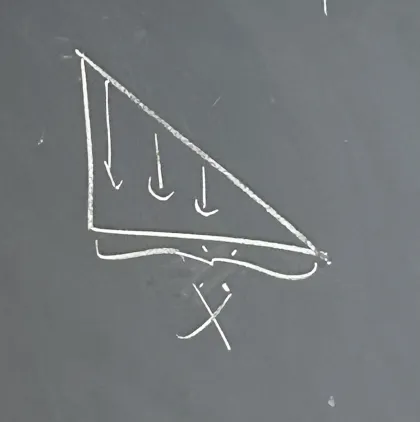
\includegraphics[width=0.25\textwidth]{Figures/right_triangle.png}\]
    This is not a fiber bundle but it is a Serre fibration.
\end{example}

\begin{remark}
    A map that is locally a Serre fibration is actually a Serre fibration. This is more involve to prove then showing that fiber bundles are Serre fibrations.
\end{remark}

\begin{definition}
    Suppose $(X, x_0)$ is a space, let $P_X = \{\gamma: I \to X| \gamma(0) = x_0\}$. There is a Serre fibration
    \[p: P_X \to P, p(\gamma) = \gamma(1), \]
    whose fiber $p^{-1}(x)$ is $\{\gamma: I \to X\ |\ \gamma(0) = x_0, \gamma(1) = x\}$. This fiber is actually homotopy equivalent to the loop space $\Omega_{x_0}$.  
\end{definition}

\begin{example}
Here are some examples of fiber bundles.
\begin{itemize}
    \item 0) If $F$ is discrete, then $p: Y \to X$ with $p^{-1}(x_0) = F$ is a covering space. For example, we can consider
    \[S^0 \to S^n \to_{p} \Rbb P^n, n \geq 2.\]
    In this case we have an LES
    % https://q.uiver.app/#q=WzAsNCxbMCwwLCJcXHBpXzEoU15uKSA9IDAiXSxbMSwwLCJcXHBpXzEoXFxSYmIgUF5uKSA9IFxcWmJiLzIiXSxbMiwwLCJcXHBpXzAoU14wKSA9IFxcWmJiLzIiXSxbMywwLCIwIl0sWzAsMV0sWzEsMl0sWzIsM11d
\[\begin{tikzcd}
	{\pi_1(S^n) = 0} & {\pi_1(\Rbb P^n) = \Zbb/2} & {\pi_0(S^0) = \Zbb/2} & 0
	\arrow[from=1-1, to=1-2]
	\arrow[from=1-2, to=1-3]
	\arrow[from=1-3, to=1-4]
\end{tikzcd}\]
    \item 1) Let $U(1)$ act on $S^{2n+1} \subseteq \Cbb^{n+1} \setminus \{0\}$ by the acton
    \[\lambda (z_0, ..., z_n) = (\lambda z_0, ..., \lambda z_n).\]
    In this case, we have that $\Cbb P^n$ are the orbits of this group action
    \[S^{2n+1}/U(1) = \Cbb P^n.\]
    Here, the map $p: S^{2n+1} \to \Cbb P^n$ is a fiber bundle. The trivializing cover is given by
    \[U_i = \{[z_0: ...: z_i: ...: z_n]\ |\ z_i \neq 0\} \subseteq \Cbb P^n,\]
    where $p^{-1}(U_i) \cong U_i \times U(1)$ is given by
    \[(z_0, ... , z_n) \mapsto ([z_0: ... : z_n], \frac{z_i}{|z_i|})\]

    From the LES of fibration, we have that
    % https://q.uiver.app/#q=WzAsMTEsWzAsMCwiXFxwaV8zKFUoMSkpID0gMCJdLFsxLDAsIlxccGlfMyhTXnsybisxfSkiXSxbMiwwLCJcXHBpXzMoXFxDYmIgUF5uKSJdLFswLDEsIlxccGlfMihVKDEpKSA9IDAiXSxbMSwxLCJcXHBpXzIoU157Mm4rMX0pIl0sWzIsMSwiXFxwaV8yKFxcQ2JiIFBebikiXSxbMCwyLCJcXHBpXzEoVSgxKSkgPSBcXFpiYiJdLFsxLDIsIlxccGlfMShTXnsybisxfSkiXSxbMiwyLCJcXHBpXzEoXFxDYmIgUF5uKSJdLFswLDMsIlxccGlfMChVKDEpKSJdLFsxLDMsIi4uLiJdLFswLDFdLFsxLDJdLFsyLDNdLFszLDRdLFs0LDVdLFs1LDZdLFs2LDddLFs3LDhdLFs4LDldXQ==
\[\begin{tikzcd}
	{\pi_3(U(1)) = 0} & {\pi_3(S^{2n+1})} & {\pi_3(\Cbb P^n)} \\
	{\pi_2(U(1)) = 0} & {\pi_2(S^{2n+1})} & {\pi_2(\Cbb P^n)} \\
	{\pi_1(U(1)) = \Zbb} & {\pi_1(S^{2n+1})} & {\pi_1(\Cbb P^n)} \\
	{\pi_0(U(1))} & {...}
	\arrow[from=1-1, to=1-2]
	\arrow[from=1-2, to=1-3]
	\arrow[from=1-3, to=2-1]
	\arrow[from=2-1, to=2-2]
	\arrow[from=2-2, to=2-3]
	\arrow[from=2-3, to=3-1]
	\arrow[from=3-1, to=3-2]
	\arrow[from=3-2, to=3-3]
	\arrow[from=3-3, to=4-1]
\end{tikzcd}\]
If we assume that $2n + 1 > 2$, then we have that $\pi_2(S^{2n+1}) = 0$. In this case, we have that
\[\pi_2(\Cbb P^n) \cong \Zbb \text{ and } \pi_k(S^{2n+1}) \cong \pi_k(\Cbb P^n) \text{ for } k > 2.\]

    \item 2) In the specific case where we look at
    \[U(1) \hookrightarrow S^3 \to \Cbb P^1 \cong S^2 \]
    We have the long exact sequence
    % https://q.uiver.app/#q=WzAsNixbMCwwLCJcXHBpXzMoVSgxKSk9MCJdLFsxLDAsIlxccGlfMyhTXjMpIl0sWzIsMCwiXFxwaV8zKFxcQ2JiIFBeMSkiXSxbMCwxLCJcXHBpXzIoVSgxKSkgPSAwIl0sWzEsMSwiXFxwaV8yKFNeMykiXSxbMiwxLCIuLi4iXSxbMCwxXSxbMSwyLCJcXGNvbmciXSxbMiwzXSxbMyw0XSxbNCw1XV0=
\[\begin{tikzcd}
	{\pi_3(U(1))=0} & {\pi_3(S^3)} & {\pi_3(\Cbb P^1)} \\
	{\pi_2(U(1)) = 0} & {\pi_2(S^3)} & {...}
	\arrow[from=1-1, to=1-2]
	\arrow["\cong", from=1-2, to=1-3]
	\arrow[from=1-3, to=2-1]
	\arrow[from=2-1, to=2-2]
	\arrow[from=2-2, to=2-3]
\end{tikzcd}\]
Here, we see that
\[\pi_3(\Cbb P^1) \cong \pi_3(S^2) = \Zbb.\]
The generator of this map $p: S^3 \to S^2$ is called the \textbf{Hopf map} (or the \textbf{Hopf fibration}).
\end{itemize}
\end{example}


Here is a general fact we should keep in mind that we will be using to construct many examples of fiber bundles.
\begin{proposition}
    If $G$ is a compact Lie group acting freely on a differentiable manifold $M$, then 
    \[p: M \to M/G\]
    is a fiber bundle.
\end{proposition}

\newpage
\section{Lecture October 15th, 2024 - Afternoon Lecture}

\subsection{The Slice Theorem}

Recall in the morning we stopped on the following proposition.
\begin{proposition}
    If $G$ is a compact Lie group acting freely on a differentiable (compact) manifold $M$, then 
    \[p: M \to M/G\]
    is a fiber bundle.
\end{proposition}

To do this, it comes from a more general theorem.
\begin{theorem}[Slice Theorem]
    Let $G$ be a compact Lie group acting on $M$, then at any point $x \in M/G$, there exists a neighborhood $U$ containing $x$ such that $$p^{-1}(U) \cong S \times_{G_x} G \coloneqq \{(s, g) \in S \times G\}/\sim .$$
    To clarify the notations
    \begin{enumerate}
        \item The equivalence relation is generated by $(sh, g) \sim (s, hg)$ for all $h \in G_x$.
        \item $G_x$ is the set of stabilizer $\{g \in G\ |\ gx = x\}$. This is sometimes called the \textbf{isotropy group}.
        \item $S \subseteq M$ is a diffeomorphism of a neighborhood of $0$ in an Euclidean space $\Rbb^k$, where $G_x$ acts by a linear representation.
    \end{enumerate}
\end{theorem}

Here is a picture to keep in mind. The ambient space is the manifold $M$ and the curve drawn in the middle is the orbit. The Slice Theorem essentially says there is a tubular neighborhood around the orbit in the original manifold that is very special (given by the description of $S$ in the theorem).
\[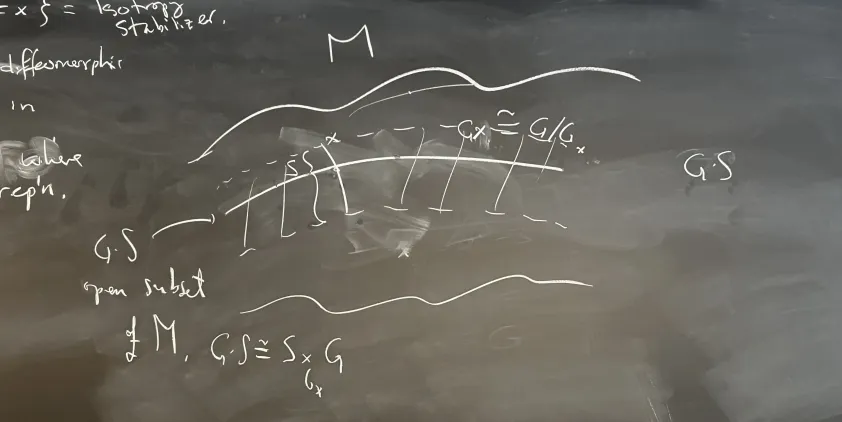
\includegraphics[width=0.5\textwidth]{Figures/slice_theorem.png}\]

In particular, if $H \subseteq G$ is a subgroup.  If there is a group homomorphism
\[H \mapsto O(V),\]
where $V$ is some Euclidean space and $O(V)$ is its orthogonal matrices. In this case, $G$ will act on
\[G \times_H V\]
These should be interpreted as local $G$-models for a compact Lie group acting on a manifold. The slice theorem says we can break up $M$ into these local models, where $H$ may vary based on the point.

\begin{example}
    Consider the action of $S^1$ on $S^2$ by rotating the equator $e$. In this case, the north and south poles are the fixed points. The orbit space is the closed interval. If you take the midpoint of the interval and look at its preimage, we have the following picture
    \[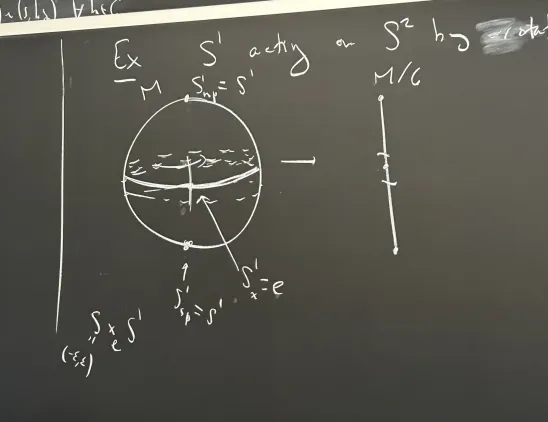
\includegraphics[width=0.5\textwidth]{Figures/spinning_earth.png}\]
    If you look at the preimage of one of the end0points though, its slice would change and span a disk over the pole in the preimage.
\end{example}

\begin{theorem}
    Given a $G$ acting on a manifold $M$, there exists a Riemannian metric which is $G$-invariant.
\end{theorem}

\begin{proof}
    Choose any Riemannian metric $g$ on $M$, we can define
    \[\Tilde{g}(x, y) = \int_{G} g(hX, hy) dh. \]
    Let us consider $(M, \Tilde{g})$ instead.
\end{proof}

\begin{proof}[Proof of Slice Theorem]
    Choose $\Tilde{g}$ on $M$ as Riemannian metric that is $G$-invariant.\\

   Now for an orbit $Gx$, we look at $N_\epsilon = \{y \in M\ |\ d(y, Gx) \leq \epsilon\}$. Note that $N_\epsilon$ is invariant under $G$ since $\Tilde{g}$ is invariant under $G$. For $\epsilon$ small enough, $N_{\epsilon}$ is the normal bundle $\nu_i$ around $Gx$. Let $i: Gx \to M$ be the inclusion map, then $Gx$ acts on the normal bundle $\nu_i$. We can choose the slice $S$ to be $v_{i, x}$ (the fiber of the normal bundle at the point $x$, under the identification between $N_{\epsilon} \cong v_i$).\\

   Note that since $Gx$ is compact, that is why we can choose $\epsilon$ small enough so that $N_\epsilon$ is the normal bundle.
\end{proof}

\begin{example}
    Here are some more examples of fiber bundles.
    \begin{enumerate}
        \item If $X$ is a differentiable manifold, its tangent and cotangent bundles $TX, T^*X$ are both fiber bundles. 
        \item The subset $SX \subseteq TX$ being vectors of length $1$ (after choosing a Riemannian metric) is a sphere bundle.
        \item Consider the fiber bundle for $\Cbb P^n$ and $\Hbb P^n$ (the quarternionic projective space)
        % https://q.uiver.app/#q=WzAsMyxbMCwwLCJVKDEpIl0sWzEsMCwiU157Mm4rMX0iXSxbMiwwLCJcXENiYiBQXm4iXSxbMSwyLCJwIl0sWzAsMSwiIiwwLHsic3R5bGUiOnsidGFpbCI6eyJuYW1lIjoiaG9vayIsInNpZGUiOiJ0b3AifX19XV0=
\[\begin{tikzcd}
	{U(1)} & {S^{2n+1}} & {\Cbb P^n}
	\arrow[hook, from=1-1, to=1-2]
	\arrow["p", from=1-2, to=1-3]
\end{tikzcd}\]

% https://q.uiver.app/#q=WzAsMyxbMiwwLCJcXG1hdGhiYntIfSBQXjIiXSxbMSwwLCJTXns0biszfSJdLFswLDAsIlNVKDIpIl0sWzIsMSwiIiwwLHsic3R5bGUiOnsidGFpbCI6eyJuYW1lIjoiaG9vayIsInNpZGUiOiJ0b3AifX19XSxbMSwwXV0=
\[\begin{tikzcd}
	{SU(2)} & {S^{4n+3}} & {\mathbb{H} P^2}
	\arrow[hook, from=1-1, to=1-2]
	\arrow[from=1-2, to=1-3]
\end{tikzcd}\]
Here, $S^{4n+3}$ sits in $\Cbb^{2(n+1)}$, and the action of $SU(2)$ is given by component wise action of $SU(2)$ on the coordinates
\[((z_0, z_1), (z_2, z_3), ..., (z_{2n+1}, z_{2n+2})).\]
Note that $SU(2)$ is isomorphic to the unit quarternions, and also note each $(z_i, z_{i+1}) \in \Cbb^2$.\\

Note that $SU(2)$ is diffeomorphic to $S^3$, so we have
\[\pi_n(SU(2)) = \pi_n(S^3) = \begin{cases}
    0, n < 3\\
    \Zbb, n = 3,\\
    ...
\end{cases}\]
Considering the long exact seqeunce, let $n \geq 1$, we have that
% https://q.uiver.app/#q=WzAsNyxbMiwxLCJcXHBpXzQoXFxIYmIgUF5uKSJdLFsxLDEsIlxccGlfNChTXns0biszfSkgPSAwIl0sWzAsMSwiXFxwaV80KFNVKDIpKSJdLFsyLDAsIi4uLiJdLFswLDIsIlxccGlfMyhTVSgyKSkgPSBcXFpiYiJdLFsxLDIsIlxccGlfMyhTXns0biszfSkgPSAwIl0sWzIsMiwiLi4uIl0sWzMsMl0sWzIsMV0sWzEsMF0sWzQsNV0sWzAsNF0sWzUsNl1d
\[\begin{tikzcd}
	&& {...} \\
	{\pi_4(SU(2))} & {\pi_4(S^{4n+3}) = 0} & {\pi_4(\Hbb P^n)} \\
	{\pi_3(SU(2)) = \Zbb} & {\pi_3(S^{4n+3}) = 0} & {...}
	\arrow[from=1-3, to=2-1]
	\arrow[from=2-1, to=2-2]
	\arrow[from=2-2, to=2-3]
	\arrow[from=2-3, to=3-1]
	\arrow[from=3-1, to=3-2]
	\arrow[from=3-2, to=3-3]
\end{tikzcd}\]
Here, we conclude that 
\[\pi_4(\Hbb P^n) = \Zbb.\]
    \end{enumerate}
\end{example}

\subsection{Constructing Fiber Bundles}

Given a fiber bundle $p: Y \to X$. For all $x \in X$, there exists a homeomorphism 
    \[\varphi_x: p^{-1}(U_x) \to U_x \times F\]
    such that
    % https://q.uiver.app/#q=WzAsMyxbMCwwLCJwXnstMX0oVV94KSJdLFsxLDAsIlVfeCBcXHRpbWVzIEYiXSxbMSwxLCJVX3giXSxbMCwyLCJwIl0sWzAsMSwiXFx2YXJwaGlfeCJdLFsxLDJdXQ==
\[\begin{tikzcd}
	{p^{-1}(U_x)} & {U_x \times F} \\
	& {U_x}
	\arrow["{\varphi_x}", from=1-1, to=1-2]
	\arrow["p", from=1-1, to=2-2]
	\arrow[from=1-2, to=2-2]
\end{tikzcd}\]
Assume for simplicity that $X$ is compact, so we can choose a finite subcover $U_{x_1}, ..., U_{x_N}$.\\

For each $i = 1, ..., N$, we have a diagram,
% https://q.uiver.app/#q=WzAsMyxbMCwwLCJwXnstMX0oVV97eF9pfSkiXSxbMSwwLCJVX3t4X2l9IFxcdGltZXMgRiJdLFsxLDEsIlVfe3hfaX0iXSxbMSwyXSxbMCwxLCJcXHZhcnBoaV97eF9pfSJdLFswLDIsInAiLDJdXQ==
\[\begin{tikzcd}
	{p^{-1}(U_{x_i})} & {U_{x_i} \times F} \\
	& {U_{x_i}}
	\arrow["{\varphi_{x_i}}", from=1-1, to=1-2]
	\arrow["p"', from=1-1, to=2-2]
	\arrow[from=1-2, to=2-2]
\end{tikzcd}\]

No suppose $i \neq j$, then we can consider the restriction of the two maps
\[\varphi_{x_i}: p^{-1}(U_{x_i} \cap U_{x_j}) \to (U_{x_i} \cap U_{x_j}) \times F.\]
\[\varphi_{x_j}: p^{-1}(U_{x_j} \cap U_{x_j}) \to (U_{x_i} \cap U_{x_j}) \times F.\]
These two maps do not have to be the same on their overlaps! We can now consider
% https://q.uiver.app/#q=WzAsMyxbMCwwLCIgcF57LTF9KFVfe3hfaX0gXFxjYXAgVV97eF9qfSkiXSxbMiwwLCIoVV97eF9pfSBcXGNhcCBVX3t4X2p9KSBcXHRpbWVzIEYiXSxbMiwxLCIoVV97eF9pfSBcXGNhcCBVX3t4X2p9KSBcXHRpbWVzIEYiXSxbMCwyLCJcXHZhcnBoaV97eF9qfSIsMl0sWzAsMSwiXFx2YXJwaGlfe3hfaX0iXSxbMiwxLCJcXHZhcnBoaV97eF9pfSBcXGNpcmMgXFx2YXJwaGlfe3hfan1eey0xfSIsMl1d
\[\begin{tikzcd}
	{ p^{-1}(U_{x_i} \cap U_{x_j})} && {(U_{x_i} \cap U_{x_j}) \times F} \\
	&& {(U_{x_i} \cap U_{x_j}) \times F}
	\arrow["{\varphi_{x_i}}", from=1-1, to=1-3]
	\arrow["{\varphi_{x_j}}"', from=1-1, to=2-3]
	\arrow["{\varphi_{x_i} \circ \varphi_{x_j}^{-1}}"', from=2-3, to=1-3]
\end{tikzcd}\]

\begin{question}
    What does the map do?
    \[\varphi_{x_i} \circ \varphi_{x_j}^{-1}: (U_{x_i} \cap U_{x_j}) \times F \to (U_{x_i} \cap U_{x_j}) \times F\]
\end{question}

We compute to see
\begin{align*}
    \varphi_{x_i} \circ \varphi_{x_j}^{-1}(x, f) &= (x, \psi_{ij}(x)(f)).
\end{align*}
The first coordinate is because of the commutativity of the diagram. On the other hand, $\psi_{ij}$ is a function dependent on the index $i$ and $j$. We can think of
\[\psi_{ij}: U_{x_i} \cap U_{x_j} \to \operatorname{Homeo}(F).\]

\begin{definition}
We say that the transition maps satisfy the cocycle condition - if given $U_{x_i}, U_{x_j}, U_{x_k}$ with $\varphi_{x_i}, \varphi_{x_j}, \varphi_{x_k}$, here we have the maps
    \[\psi_{ij} = \varphi_{x_i} \circ \varphi_{x_j}^{-1}: U_{x_i} \cap U_{x_j} \to \operatorname{Homeo}(F)\]
    \[\psi_{jk} = \varphi_{x_j} \circ \varphi_{x_k}^{-1}: U_{x_j} \cap U_{x_k} \to \operatorname{Homeo}(F).\]
    \[\psi_{ik} = \varphi_{x_i} \circ \varphi_{x_k}^{-1}: U_{x_i} \cap U_{x_k} \to \operatorname{Homeo}(F).\]
    On $U_{x_i} \cap U_{x_j} \cap U_{x_k}$, we have that
    \[\psi_{ij} \circ \psi_{jk} = \psi_{ik}.\]
    This is called the \textbf{cocycle condition}. Note that clearly $\psi_{ii}$ is the identity on $F$ for all $x \in U_{x_i}$.
\end{definition}

Note that everything we said works just as well for an arbitrary cover.

\begin{proposition}
Let $p: Y \to X$ be a fiber bundle with fiber $F$, for any trivializing cover $U_{\alpha}$, $\psi_{\alpha \beta}: U_{\alpha} \cap U_{\beta} \to \operatorname{Homeo}(F)$ satisfying the cocycle condition.
\end{proposition}
    
We can also go backwards on this. 
\begin{definition}
    Given a collection of $U_{\alpha}$ covering $X$ with maps $\psi_{\alpha \beta}: U_{\alpha, \beta} \to \operatorname{Homeo}(F)$ satisfying the cocycle condition, we can construct a fiber bundle $Y$ as follows.
    \[Y = \bigsqcup U_{\alpha} \times F/\sim\]
    where $(x, f) \in U_{\alpha \beta} \times F \subseteq U_{\beta} \times F$ is identified by $(x, \psi_{\alpha \beta}(f)) \in U_{\alpha \beta} \times F \subseteq U_\alpha \times F$. The map $Y \to X$ is the projection map to the first coordinate.
\end{definition}

\subsection{$(G, F)$ fiber-bundles}

In the construction of fiber bundles, we were concerned with $\operatorname{Homeo}(F)$, but we can get richer structure when we restrict to specific subgroups of $\operatorname{Homeo}(F)$.

\begin{definition}
    Let $G$ be a topological group. Suppose $G$ is acting on a space $F$ with a left action
    \[G \times F \to F, (g, f) \mapsto g \cdot f.\]
    This can be though off as a map $G \to \operatorname{Homeo}(F)$. We also suppose this map is injective (ie. action is faithful).\\ 
    
    A $(G, F)$-fiber bundle is a fiber bundle $p: Y \to X$ such that there exists an open cover $\{U_\alpha\}$ of $X$ and
    \[\varphi_{\alpha}: p^{-1}(U_{\alpha}) \to U_{\alpha} \times F\]
    such that the corresponding transition functions $\psi_{\alpha \beta}: U_{\alpha, \beta} \to \operatorname{Homeo}(F)$ lands in $G \subseteq \operatorname{Homeo}(F)$ (identified with the image of $G \to \operatorname{Homeo}(F)$).
\end{definition}

\begin{remark}
What we have shown previously shows that there is a $1-1$ correspondence between a $(G, F)$-fiber bundle and a collection of open maps $\{U_{\alpha}\}$ and transition maps $\psi_{\alpha \beta}: U_{\alpha \beta} \to G$ satisfiying the identity condition and the cocycle condition. To emphasize the presence of the group $G$, we sometimes also use $g_{\alpha \beta}: U_{\alpha \beta} \to G$ to mean the transition maps.\\

The general \textbf{slogan} is as follows - if $G$ preserves some structure on $F$, then the $(G, F)$-bundles will have that structure.
\end{remark}

\begin{example}
    Let us suppose $G = GL_{n}(\Cbb)$ and $F = \Cbb^n$, where $G$ acts on $F$ by how matrices usually act. In this case, $G$ preserves the vector-space structure on $F$. In this case, when we construct a $(G, F)$-fiber bundle for
    \[Y = \bigsqcup U_\alpha \times F/\sim, (x, f) \sim (x, g_{\alpha \beta}(x)(f)).\]
    The element $g_{\alpha \beta}(x)$ is an element of $GL_{n}(\Cbb)$, and this will give the structure of a complex vector space on the fiber $F$. Thus, $Y \to X$ is exactly a complex vector-bundle. If we instead use $G = U(n)$ and $F = \Cbb^n$, $G$ preserves the vector space structure and the Hermitian structure on $\Cbb^n$. Then the associated $(G, F)$-fiber bundle is exactly a complex vector-bundle equipped with a Hermitian metric.
\end{example}

\begin{example}
     If we instead use $G = GL_n(\Rbb)$ and $F = \Rbb^n$, a $(G, F)$-bundle is exactly a real vector bundle. If we instead use $G = O(n)$ and $F = \Rbb^n$, we get a real vector bundle equipped with a inner product.
\end{example}

\begin{example}
    There is an act of $G$ on $G$ by left-multiplication. A $(G, G)$-bundle is called a \textbf{principal $G$-bundle}. Suppose $\pi: P \to X$ is a principal $G$-bundle. The action of $G$ on $G$ is not an automorphism of $G$ (left multiplication is not a group homomorphism), so the fibers of $X$ will not have a group structure as $G$ (as there is no canonical way to choose an identity element). These fibers are examples of what is called a \ul{$G$-torsor} - which is a space $X$ that is isomorphic to $G$, but not canonically. They arise for instance from principal $G$-space (meaning it is free and transitive).\\
    
    The action of $G$ on $G$ is principal, so there are free-transitive actions on the fibers of $X$ and the fibers are principal $G$-spaces.\\

    Given a principal $G$-set $G$, and let $x_0 \in G$, we can give a group structure on $G$ with $x_0$ as the identity as follows. For $x, y \in G$, we can define
    \[x \cdot y \coloneqq x \cdot_G (x_0^{-1} y).\]
    Here $x \in G$ acts on $x_0^{-1} y \in G$ by left multiplication.\\

    If we can choose a section $s: X \to P$, then we could turn $P$ into a group-bundle where each fiber over $x$ is given a group structure structure with identity $s(x)$. But it turns out if we have a section, then the bundle has to be trivial! (this is very different for the case of vector bundles). This is because we can explicitly define a $(G, G)$-isomorphism of fiber bundles as follows
    \[P \to X \times G, y \mapsto (\pi(y), g_{y}).\]
    Here $g_{y} \in G$ is defined as follows. $y$ and $s(\pi(y))$ are both elements in the same fiber, and there exists a unique element $g_y$ such that $g_y \cdot y = s(\pi(y))$.
\end{example}


\newpage
\section{Lecture October 22th, 2024 - Morning Lecture}

\subsection{Principal $G$-bundles}

We will first talk about a specific example. Let us first recall the definition.

\begin{definition}
    Let $G$ be a Lie group, $F$ be a topological space, and $G$ acts on $F$ by a left $G$-action:
    \[G \times F \to F.\]
    Another way to think of this is a map
    \[\alpha: G \to \operatorname{Homeo}(F).\]
    Given $p: Y \to X$, we say that \ul{$p: Y \to X$ is a $(G, F)$-bundle} if there exists a cover $U_{\alpha}$ of $X$ and homeomorphisms
    \[\varphi_\alpha: p^{-1}(U_{\alpha}) \to U_\alpha \times F, \]
    such that the following diagram commutes
    % https://q.uiver.app/#q=WzAsMyxbMCwwLCJwXnstMX0oVV9cXGFscGhhKSJdLFsyLDAsIlVfXFxhbHBoYSBcXHRpbWVzIEYiXSxbMSwxLCJVX1xcYWxwaGEiXSxbMCwxLCJcXHZhcnBoaV9cXGFscGhhIl0sWzAsMiwicCIsMl0sWzEsMl1d
\[\begin{tikzcd}
	{p^{-1}(U_\alpha)} && {U_\alpha \times F} \\
	& {U_\alpha}
	\arrow["{\varphi_\alpha}", from=1-1, to=1-3]
	\arrow["p"', from=1-1, to=2-2]
	\arrow[from=1-3, to=2-2]
\end{tikzcd}\]
From here we define the transition maps $g_{\alpha \beta}$ as the composition
% https://q.uiver.app/#q=WzAsNCxbMCwwLCJnX3tcXGFscGhhIFxcYmV0YX06Il0sWzEsMCwiVV97XFxhbHBoYSBcXGJldGF9IFxcdGltZXMgRiJdLFsyLDAsInBeey0xfShVX3tcXGFscGhhIFxcYmV0YX0pIl0sWzMsMCwiVV97XFxhbHBoYSBcXGJldGF9IFxcdGltZXMgRiJdLFsxLDIsIlxcdmFycGhpX1xcYmV0YV57LTF9Il0sWzIsMywiXFx2YXJwaGlfXFxhbHBoYSJdXQ==
\[\begin{tikzcd}
	{g_{\alpha \beta}:} & {U_{\alpha \beta} \times F} & {p^{-1}(U_{\alpha \beta})} & {U_{\alpha \beta} \times F}
	\arrow["{\varphi_\beta^{-1}}", from=1-2, to=1-3]
	\arrow["{\varphi_\alpha}", from=1-3, to=1-4]
\end{tikzcd}\]
Here $U_{\alpha \beta} = U_\alpha \cap U_\beta$. From the commutativity of the diagram before, we can think of
\[g_{\alpha \beta}: U_{\alpha \beta} \times F \to U_{\alpha \beta} \times F, g_{\alpha \beta}(x, f) = (x,  g_{\alpha \beta}(x) \cdot f).\]
We use a slight abuse of notation here to use $g_{\alpha \beta}: U_{\alpha \beta} \to G \subseteq \operatorname{Homeo}(F)$ to also denote how $f \in F$ is sent to within $F$.\\

We also note that the transition maps satisfy the \textbf{cocycle condition} on $U_{\alpha \beta \gamma}$:
\[g_{\alpha \beta} \circ g_{\beta \gamma} = g_{\alpha \gamma}.\]
Further more on $U_{\alpha}$, we have the \textbf{identity condition}
\[g_{\alpha \alpha} = id.\]

In the specific case where $F = G$ where $G$ acts on $G$ by left-multiplication, the $(G,G)$-fiber bundle is also called a \ul{principal $G$-bundle}.
\end{definition}

% For a principal $G$-bundle $p: P \to X$, we have homeomorphisms
% \[\varphi_{\alpha}: p^{-1}(U_\alpha) \to U_\alpha \times G\]
% and $g_{\alpha \beta} = \varphi_\alpha \circ \varphi_\beta^{-1}: U_{\alpha \beta} \times G \to U_{\alpha \beta} \times G$ gives $g_{\alpha \beta}: U_{\alpha \beta} \to G$.\\

We first observe that there is a following equivalent definition of principal $G$-bundle as follows:
\begin{definition}[Alternative Construction]
    Let $\pi: P \to B$ be a fiber bundle with fiber $X$, and let there be a continuous right $G$-action $P \times G \to P$ that preserves the fibers of $\pi$ and acts principally (transitively and freely) on the fibers. For each fiber $\pi^{-1}(b)$, the restriction of the action gives a map $\pi^{-1}(b) \times G \to \pi^{-1}(b)$ for each $b \in B$.\\

    Fix $x_0 \in \pi^{-1}(b)$, we can construct a continuous map
    \[\phi_{x_0}: G \to \pi^{-1}(b), g \mapsto x_0 g. \]
    This map is surjective because the action is transitive. This map is injective because the action is free. We furthermore require that $\phi_{x_0}$ is a homeomorphism (\textbf{Note: }Under reasonable hypothesis, if $G$ is compact and $X$ is Hausdorff, then this is automatically satisfied. This may be relaxed to specifying the action of $G$ is proper and the fiber is CGWH, in which case $\phi$ would become a closed map.).\\

    If these hypothesises are all satisfied, we call $\pi: P \to B$ a principal $G$-bundle. Note that for a principal $G$-bundle define in this alternative definition, it is very apparently that the taking the $G$-orbits gives a homeomorphism
    \[P/G \cong B.\]
\end{definition}

\begin{proposition}
    On reasonable spaces, the two constructions of principal $G$-bundle can be recovered from each other.
\end{proposition}

\begin{proof}
\textbf{To go from the first definition to the second,} let us look at a general $(G,F)$-bundle first. Suppose we have a $(G, F)$-bundle $\pi: P \to B$ and we have identified $G \subseteq \operatorname{Homeo}(F)$. Consider the trivialization maps and transition maps
\[\varphi_{\alpha}: \pi^{-1}(U_{\alpha}) \to U_{\alpha} \times F \]
\[\psi_{\alpha \beta}: U_{\alpha \beta} \times F \to U_{\alpha \beta} \times F, (x, f) \mapsto (x, g_{\alpha \beta}(x) \cdot f).\]
Now, $G$ has a left action on the fiber $F$ coming from the definition. Let us go with the thought experiment and suppose that $G$ also has right action on the fiber $F$, which is not necessarily the same as the left action.\\

We can attempt to construct a right action of $G$ on $P$ as follows. For each fiber $F_b \coloneqq \pi^{-1}(b)$, there is a right action of $G$ on $F_b$ given as follows - for $x \in F_b$, then
\[x \cdot g \coloneqq \varphi_{\alpha}^{-1}(b, (\pi_2 \circ \varphi_{\alpha}(x)) \cdot g). \]
Here $\pi_2$ is the projection of $U_{\alpha} \times F$ onto $F$, and it is given by the natural right action indicated above.\\

Note that this satisfies composition because for $g, h \in G$,
\begin{align*}
    (x \cdot g) \cdot h &= \varphi_{\alpha}^{-1}(b, (\pi_2 \circ \varphi_{\alpha}(x \cdot g)) \cdot h)\\
    &= \varphi_{\alpha}^{-1}(b, (\pi_2 \circ \varphi_{\alpha}(\varphi_{\alpha}^{-1}(b, (\pi_2 \circ \varphi_{\alpha}(x))) \cdot g) \cdot h))\\
    &= \varphi_{\alpha}^{-1}(b, (\pi_2 \circ \varphi_\alpha(x))\cdot g) \cdot h))\\
    &= \varphi_{\alpha}^{-1}(b, (\pi_2 \circ \varphi_{\alpha}(x)) \cdot gh )\\
    &= x \cdot gh.
\end{align*}
Thus, we have defined a valid group action, but the question is - \textbf{is this action well-defined?}\\

Indeed, suppose $x \in U_{\alpha \beta}$, then we also want to check that
\[ \varphi_{\alpha}^{-1}(b, (\pi_2 \circ \varphi_{\alpha}(x)) \cdot g) =  \varphi_{\beta}^{-1}(b, (\pi_2 \circ \varphi_{\beta}(x)) \cdot g)\]
Indeed, we proceed to compute that
\begin{align*}
   \varphi_{\beta} \circ \varphi_{\alpha}^{-1}(b, (\pi_2 \circ \varphi_{\alpha}(x)) \cdot g) &= (b, g_{\beta \alpha}(x)(b) \cdot (\pi_2 \circ \varphi_{\alpha}(x)) \cdot g)
\end{align*}
Here we think of $g_{\beta \alpha}(x)(b)$ as an element of $G$. We observe that if the following equality is true
\[g_{\beta \alpha}(x)(b) \cdot (\pi_2(\varphi_{\alpha}(x)) \cdot g) = (g_{\beta \alpha}(x)(b) \cdot \pi_2(\varphi_{\alpha}(x))) \cdot g\quad (\dagger). \]
That is, if the left multiplication and the right multiplication structure commutes with each other, then we are good. In general, the two multiplication actions need not commutes.\\

However, when we look at a $(G, G)$-bundle (ie. $F = G$) in the first defintion of a principal $G$-bundle, the left multiplication action is the group multiplication from the left, and the right multiplication is also the group multiplication from the right. Thus, the equality in $(\dagger)$ is true, and we have that
\begin{align*}
   \varphi_{\beta} \circ \varphi_{\alpha}^{-1}(b, (\pi_2 \circ \varphi_{\alpha}(x)) \cdot g) &= (b, (g_{\beta \alpha}(x)(b) \cdot \pi_2(\varphi_{\alpha}(x))) \cdot g)\\
   &= (b, \varphi_{\beta}(x) \cdot g)
\end{align*}
Thus, we have produced a well-defined right group action on $P$, which satisfies all the desired properties mentioned.\\

\textbf{Conversely, if we want to go back from the second definition to the first definition}. Let $\pi: P \to B$ be a principal $G$-bundle in the sense of the second definition with fiber $X$. Fix $x_0 \in X$, for each $U_{\alpha} \times X$, we can produce a homeomorphism
\[\psi_{x_0}^{-1}: U_{\alpha} \times X \to U_{\alpha} \times G, (b, x) \mapsto (b, \phi_{x_0}^{-1}(x)).\]
Here $\phi_{x_0}$ is the fiber wise homeomorphism outlined in the second definition. We claim that the maps $\psi_{x_0}^{-1} \circ \varphi_{\alpha}: \pi^{-1}(U_{\alpha}) \to U \times G$ gives $\pi: P \to B$ the structure of a $(G, G)$-fiber bundle. It suffices for us to check that the corresponding transition maps act like group multiplication on the left.\\

Indeed, for any $(b, g) \in U_{\alpha} \times G$, we check that
\begin{align*}
  (\psi_{x_0}^{-1} \circ \varphi_{\beta}) \circ (\psi_{x_0}^{-1} \circ \varphi_{\alpha})^{-1} (b, x_0 g) &= \psi_{x_0}^{-1} \circ \varphi_{\beta} \circ \varphi_{\alpha}^{-1} \circ \psi_{x_0}(b, g)\\
  &= \psi_{x_0}^{-1} \circ \varphi_{\beta} \circ \varphi_{\alpha}^{-1}(b, x_0 g)\\
  &= \psi_{x_0}^{-1}(b,  g_{\beta \alpha}(b) (x_0 g))\\
  &= \psi_{x_0}^{-1}(b,  g_{\beta \alpha}(b)(x_0) g) \tag*{$G$ acts equivariantly with respect to $g_{\beta \alpha}$}\\
  &= \psi_{x_0}^{-1}(b, (x_0 \cdot h_{\beta \alpha}) g) \tag*{We can represent the element $g_{\beta \alpha}(b)(x_0)$ uniquely as $x_0 \cdot h_{\beta \alpha}$ because action is principal }\\
  &= \psi_{x_0}^{-1}(b, (x_0 \cdot h_{\beta \alpha} g)\\
  &= (b, h_{\beta \alpha} g).
\end{align*}
We see that the transition maps act on the fibers exactly by left multiplication. This concludes the converse direction.
\end{proof}

% For a $(G, F)$-bundle, the trivialization maps is equivariant with respect to the left action of $G$ on $F$ in the sense that
% \[\varphi_{\alpha}^{-1}(x, g \cdot f) = \]

% For a principal $G$-bundle $\pi: P \to X$. There is a natural right $G$-action on $P$. 

% In general, let $X$ be a principal $G$-space, ie. a space $X$ with a transitive free $G$-action. By choosing a point $x_0 \in X$, we get a homeomorphism of $X$ with $G$ given by
% \[\phi_{x_0}: G \to X, g \mapsto g \cdot x_0.\]
% (Transitively implies surjectivity, freeness imply injectivity).\\

% Now, $X$ has a \textbf{\ul{canonoical right $G$-action}},
% \[X \times G \to X \]
% constructed as follows:
% \begin{enumerate}
%     \item $X \times G$ is isomorphic to $G \times G$ as explained above.
%     \item The natural binary operation on $G \times G$ gives a map
%     \[G \times G \to G, (g, g') \mapsto g g',\]
%     and $G$ is again isomorphic to $X$.
%     \item Thus, the action is given by
%     \[(x, g) \mapsto (\phi_{x_0}^{-1}(x), g) \mapsto \phi_{x_0}^{-1}(x) g \mapsto \phi_{x_0}(\phi_{x_0}^{-1}(x) g) = (\phi_{x_0}^{-1}(x) g) \cdot x_0. \]
%      This map is actually independent of $x_0$ by associativity. To see this, let $x = a \cdot x_0$ and $x = b \cdot x_1$, then
%      \begin{align*}
%          (\phi_{x_0}^{-1}(x) g) \cdot x_0 &= (ag) \cdot x_0
%      \end{align*}
% \end{enumerate}

\begin{remark}
    In algebra, if $M$ is a left $R$-module, $N$ is a right $R$-module, then $M \otimes_R N$ has a (bi)-$R$-module structure. What we are trying to do here is similar.
\end{remark}

Now that we have established a canonical right action on principal $G$-bundles, we are ready to define the notion of associated bundles.

\begin{definition}[Associated Bundles]
    If $\pi: P \to X$ is a principal $G$-bundle, and $G$ acts on $F$ on the left, then the \textbf{associated bundle} is a $(G, F)$-bundle is given by
\[\begin{tikzcd}
	F & {P \times_G F} & X
	\arrow[from=1-1, to=1-2]
	\arrow["\pi", from=1-2, to=1-3]
\end{tikzcd}\]
where $P \times_G F$ is $P \times F/\sim$ with the equivalence relation
\[(pg, f) \sim (p, g \cdot f).\]
Here the right action of $g$ on $P$ is given by the discussions above. The left action on $F$ is the usual action.
\end{definition}

\begin{proposition}
    $P \times_G F$ is a $(G, F)$-bundle. Furthermore, if the maps $\alpha: G \to \operatorname{Homeo}(F)$ is injective (these actions are called faithful/effective), then we can associate to every $(G, F)$-bundle a principal $G$-space.\\

    Note that we actually required the maps to be injective already in the previous lecture, but indeed there is a more general notion of $(G,F)$-bundle where it is not injective.
\end{proposition}

\begin{proof}
    The verifications for the first statement are omitted. For the second statement, this is because we can now identify $G$ with a subgroup of $\operatorname{Homeo}(F)$. Given $p: Y \to X$ a $(G, F)$-bundle, we can get the maps (because $G$ is now in $\operatorname{Homeo}(F)$)
    \[g_{\alpha \beta}: U_{\alpha \beta} \to G.\]
    From here, we can form a principal $G$-bundle whose transition functions $g_{\alpha \beta}$ on $\bigsqcup_{\alpha} U_\alpha \times G/\sim$ with the equivalence relation
    \[(x, g) \in U_{\alpha \beta} \times G \subseteq U_{\beta} \times G \sim (x, g_{\alpha \beta}(x) \cdot g) \in U_{\alpha \beta} \times G \subseteq U_{\alpha} \times G.\]
\end{proof}

Here is an example.
\begin{example}
    Let $M^n$ be a differentiable manifold and $P$ be the bundle of frames in $TM$, ie.
    \[P = \{ (s_1, ..., s_n) | s_i \in T_x M, x \in M, \text{$\{s_1, ..., s_n\}$ forms a basis of $T_x M$} \},\]
    In other words, $P$ is a bundle of basis for tangent spaces over $X$. This is called the \textbf{frame bundle of $M$}.\\

    The projection map $p: P \to M$ is given by $s = (s_1, ..., s_n) \to x$, and the fiber $p^{-1}(x)$ is the space of basis of $T_x M$. The space of basis of $T_x M$ can be identified  as $GL(T_x M)$ (you can always get from a fixed basis to every other basis by an invertible matrix, uniquely).\\

    $p: P \to M$ is a principal $GL_n(\Rbb)$-bundle, and $GL_{n}(\Rbb)$ acts on $\Rbb^n$ linearly. The associated bundle constructed from this principal $GL_n(\Rbb)$-bundle is $P \times_{GL_n(\Rbb)} \Rbb^n$, \textbf{which turns out to be isomorphic to the tangent bundle $TM$}.\\

    If we instead consider the action of $GL_{n}(\Rbb)$ acts on the exterior algebra $\Lambda^k (\Rbb^n)^*$ (here $(\Rbb^n)^*$ is the dual), then the associated bundle is
    \[P \times_{GL_n(\Rbb)} \Lambda^k (\Rbb^n)^* \cong \Lambda^k T^*M.\]
    In other words, it is the bundle of $k$-differential forms $\Lambda^k T^*M$.
\end{example}

\begin{remark}
    Although we will not discuss this in the class, you can actually define connections on a principal $G$-bundle.
\end{remark}

\begin{proposition}
    If $\pi: P \to X$ is a principal $G$-bundle, and if $\pi$ has a section $s: X \to P$ (ie. $\pi \circ s = id_X$), then $P$ is trivial (ie. $P$ is isomorphic to $X \times G$). 
\end{proposition}

\begin{proof}
    Let $s: X \to P$ a section, then $\pi \circ s = id_X$. On the other hand, we consider $s \circ \pi(f), f \in P$. Write $x = \pi(f)$, then $f$ and $s \circ \pi(f)$ belong in the same fiber $\pi^{-1}(x)$, which implies that there exists $g \in G$, such that
    \[s \circ \pi(f) = f \cdot g.\]
    % \begin{remark}
    %     The canonical right action of $G$ on $P$ maps each fiber homeomorphically onto itself.
    % \end{remark}
    Thus, we define a map
    \[P \to X \times G, f \mapsto (\pi(f), g).\]
    This defines an isomorphsim of $P$ with $X \times G$.
\end{proof}

\begin{example}
    For example, if $s: M \to \operatorname{Frame}$-bundle as before of $M$ is a section. This means that $s(x)$ is a basis of $x$ for all $x$. This means that we can form a map
    \[M \times \Rbb^n \to TM, (x, (\lambda_1, ..., \lambda_n)) \mapsto \lambda_1 s_1(x) + ... + \lambda_n s_n(x)\]
    which is a trivialization of $TM$, which induces a trivialization of the frame bundle.
\end{example}

\begin{definition}
    A map of principal $G$-bundles over the same base space $X$ is a morphism $\Phi: P_1 \to P_2$ such that the diagram 
    % https://q.uiver.app/#q=WzAsMyxbMCwwLCJQXzEiXSxbMSwwLCJQXzIiXSxbMCwxLCJYIl0sWzAsMiwiXFxwaV8xIl0sWzEsMiwiXFxwaV8yIl0sWzAsMSwiXFxQaGkiXV0=
\[\begin{tikzcd}
	{P_1} & {P_2} \\
	X
	\arrow["\Phi", from=1-1, to=1-2]
	\arrow["{\pi_1}", from=1-1, to=2-1]
	\arrow["{\pi_2}", from=1-2, to=2-1]
\end{tikzcd}\]
commutes, and it commutes with the right $G$-action.
\end{definition}

\begin{corollary}
    If $\Phi: P_1 \to P_2$ is a morphism of principal $G$-bundles, then $\Phi$ is an isomorphism.
\end{corollary}

\begin{proof}
    Although this was left as an exercise, we will outline the proof here. In the specific case where $P_1$ and $P_2$ are both trivial bundles $X \times G$, then
    \[\Phi(x, g) = (x, \phi(x) g)\]
    where $\phi(x) \in G$ is some element depending continuously on $x$. Now we can consider an inverse $\Psi: P_2 \to P_1$ given by
    \[\Psi(x, g) = (x, \phi(x)^{-1} g).\]
    Clearly this also commutes with the right $G$-action and is an inverse. Thus, $\Phi$ gives an isomorphism. The general case follows from a local trivialization argument and being careful of compatibility issues.
\end{proof}

From here, we are motivated to give the following definition.
\begin{definition}
    Let $P_G(X)$ be the category of $G$-principal bundles over $X$. Note from our previous discussion, $P_G(X)$ is a category whose morphisms are all isomorphhisms, and thus $P_G(X)$ is a \textbf{groupoid}. 
\end{definition}

\begin{question}
    Our goal is to ``calculate" $P_G(X)$ modulo isomorphisms in homotopy theoretic terms.
\end{question}

\subsection{Simplicial Techniques}

This is a generalization of simplicial complexes.

\begin{definition}
    $\Delta$ (or $\operatorname{Ord}$) is the category with one object $[n]$ for every $n = 0, 1, 2, ...$. The collection of morphisms are
    \[\Delta([n], [m]) = \text{order-preserving maps from } \{0, 1, ..., m\} \to \{0, 1, ..., m\}.\]
    There are special morphisms that generate the category known as face maps and degenerate maps. The face maps are of the form
    \[\partial_i: [n] \to [n+1], \partial_i(k) = \begin{cases}
        k, k < i\\
        k+1, k \geq i
    \end{cases}.\]
    In other words, these are the order preserving injections from $[n] \to [n+1]$. The degenerate maps are of the form
    \[s_i: [n] \to [n-1], s_i \text{ is the order preserving map where $k \in \{0, ..., n-1\}$ get hit twice}.\]
    Together the face maps and degeneracy maps generate all non-identity morphisms in the category. Here is a pictorial representation 
    \[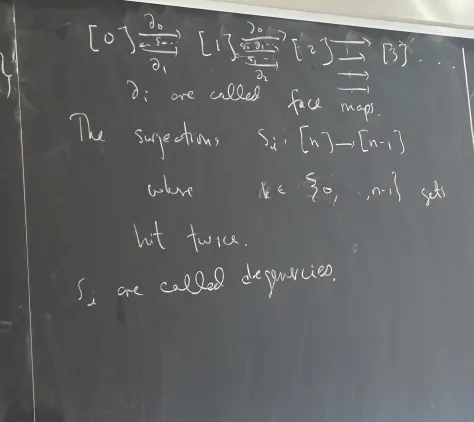
\includegraphics[width=0.5\linewidth]{Figures/simplicial_set_diag.png}\]
\end{definition}

\begin{definition}
    Let $\mathcal{C}$ be a category. A \textbf{simplicial $\Ccal$-object} is a functor from $\Delta^{op} \to \mathcal{C}$ (in other words a contravariant functor from $\Delta \to \mathcal{C}$).
\end{definition}

\begin{example}
    A simplicial set $X_{\bullet}$ is a functor $X: \Delta^{op} \to \operatorname{Set}$. Here we write
    \[X_0 = X[0], X_1 = X[1], X_2 = X[2], ...\]
    Here the face maps go from $X_i \to X_{i-1}$ and the degeneracy maps go from $X_{i-1} \to X_i$ (ie. their directions are backwards).
\end{example}

\begin{example}
    Let $K$ be a simplicial complex. For our purposes, we want to think of $K$ as a set of vertices with, for each $n$, $\Sigma^n$ is some collection of sub multi-ets (this means we allow multiple entries which are thought of degenerate simplicies) with $n+1$ elements in $K$, such that
    \begin{itemize}
        \item If $\sigma \in \Sigma^n$ and $\tau \subseteq \sigma$, then $\tau \in \Sigma^m$ for some $m \leq n$. 
    \end{itemize}
    From here, we can define a simplicial set as follows (which depends on some choice):
    \begin{itemize}
        \item Choose an arbitrary total ordering on the vertices of $K$.
        \item Let $K_n = \{(v_0, ..., v_n)\ |\ (v_0, v_1, ..., v_n) \in \Sigma^n, v_0 \leq .... \leq v_n\}$ be the set of ordered $n$-simplices.
        \item From here we define $\partial_i: K_n \to K_{n-1}$ to be given by
        \[\partial_i([v_0, ..., v_n]) = [v_1, ..., \hat{v_i}, ..., v_n].\]
        Analogously $s_i: K_{n-1} \to K_n$ to be given by
        \[s_i([v_0, ..., v_{n-1}]) = [v_0, ..., v_i, v_i, ..., v_{n-1}].\]
    \end{itemize}

    To see an example, consider the following diagram:
   \[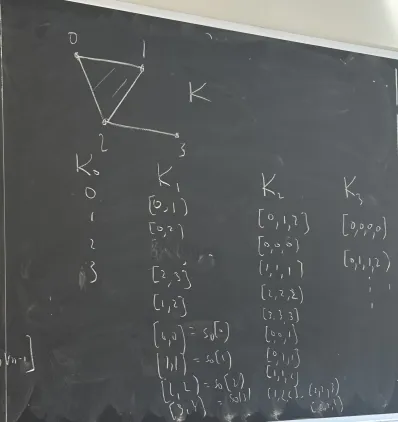
\includegraphics[width=0.5\linewidth]{Figures/simplicial_set_geo.png}\]
   Note that we allow simplicies with repeated indices to accommodate for degeneracies.
\end{example}

\begin{definition}
    A morphism from a simplicial $\Ccal$-object $F$ to another simplicial $\Ccal$-object $G$ is a natural transformation between the associated functors. More explicitly, they are just a collection of maps $h_i: F_i \to G_i$ that commutes with all associated maps given by the base categories under the functor. We use $sSet$ to denote the category of simplicial sets.
\end{definition}

\begin{definition}
     We define a covariant functor from $\operatorname{Ord} \to Top$ given as follows. For each $[n]$, we let its corresponding space $\Delta^n$ be the space
    \[\Delta^n \equiv = \{(t_0, t_1, ..., t_n) \in \Rbb^n \ |\ t_i \geq 0, \sum_{i=0}^n t_i = 1\}.\]
    We can define $\partial_i: \Delta^n \to \Delta^{n+1}$
    \[\partial_i(t_0, ..., t_n) = (t_0, ..., 0, ..., t_n)\]
    where we put $0$ at the $i$-th face. Similarly, we can define $s_i: \Delta^n \to \Delta^{n-1}$ as
    \[s_i(t_0, ..., t_n) = (t_0, ..., t_i + t_{i+1}, ..., t_n).\]
    We want to emphasize that this is a COVARIANT functor, so the directions are not flipped.
\end{definition}

\begin{definition}
    There is a functor $|\bullet|: sSet \to Top$ as follows - if $X_{\bullet}$ is a simplicial set, then
    \[|X_\bullet| = \bigsqcup_n X_n \times \Delta^n/\sim,\]
    the identification is given by - if $x \in X_n$ and $t \in \Delta^{n-1}$, then
    \[(\partial_i x, t) \sim (x, \partial_i t)\]
    if $x \in X_{n-1}, t \in \Delta^n$, then
    \[(s_i x, t) \sim (x, s_i t).\]
    The space $|X_\bullet|$ is a topological space, and it in fact turns out to be a CW-complex.
\end{definition}


\newpage
\section{Lecture October 22th, 2024 - Afternoon Lecture}

\subsection{Universal Principal $G$-bundles}

So far, we have two perspectives of principal $G$-bundles going on.
\begin{enumerate}
    \item $(G, G)$-fiber bundle.
    \item A map $\pi: P \to X$ with a free right $G$-action on $P$ such that $\pi(p \cdot g) = \pi(p)$. $G$ takes fiber to fiber and acts freely, transitively, and homeomorphically on each fiber.
\end{enumerate}
In particular, the second definition implies that the induced map
\[\pi': P/G \to X \text{ is a homeomorphism}.\]

Thus, to construct principal $G$-bundles, we should want to construct a space $P$ with a right free $G$-action, such that
\[\pi': P \to P/G \text{ is a fiber bundle}.\]

\begin{example}[Non-Example]
    Let $G = \Zbb$ act on $S^1$ by $1 \in \Zbb$ acting by rotation by $e^{2\pi i \alpha}$ for some fixed $\alpha \notin \Qbb$. This is a free action, but the quotient topology on $S^1/\Zbb$ is trivial (ie. it has only two open sets, the entire set and the set itself, because the orbits are dense) and the map $\pi: S^1 \to S^1/\Zbb$ is clearly not a fiber bundle..
\end{example}

The \textbf{good news} is as follows.
\begin{proposition}
If $G$ is compact and acts differentiably on $P$, then $\pi: P \to P/G$ is a fiber bundle.    
\end{proposition}

\begin{definition}
    A universal $G$-principle bundle is a $G$-principle bundle $E \to B$ such that for any $G$-principle bundle $P \to X$, there exists an unique homotopy class of maps $f: X \to B$ such that $P$ is the pullback $f^*(E)$:
    % https://q.uiver.app/#q=WzAsNCxbMSwwLCJFIl0sWzEsMSwiQiJdLFswLDEsIlgiXSxbMCwwLCJQIFxcY29uZyBmXiooRSkiXSxbMCwxXSxbMywyLCJcXHBpIiwyXSxbMiwxLCJmIiwyXSxbMywwXV0=
\[\begin{tikzcd}
	{P \cong f^*(E)} & E \\
	X & B
	\arrow[from=1-1, to=1-2]
	\arrow["\pi"', from=1-1, to=2-1]
	\arrow[from=1-2, to=2-2]
	\arrow["f"', from=2-1, to=2-2]
\end{tikzcd}\]
Here we assume $X$ is a CW complex, but the construction works onto the generality of paracompact spaces. We also write the universal bundle as $\pi: EG \to BG$ to emphasize the group.
\end{definition}

\begin{theorem}[Recognition Principle]
    If $\pi: E \to B$ is a principle $G$-bundle such that $E$ is contractible, then $\pi$ is a universal $G$-principle bundle. Furthermore, $E \to B$ is unique up to homotopy if $B$ is a CW-complex.
\end{theorem}

\begin{example}
Here are some examples of universal $G$-principal bundles.
    \begin{enumerate}
        \item If $G = \Zbb$, then $E = \Rbb, B = S^1$ is a universal $\Zbb$-principle $G$-bundle.
        \item If $G = \Zbb/n\Zbb$, then take $E = S^{\infty}$, $B = L(n, \infty)$ (being the infinite dimensional Lens space corresponding to $n$). Let us recall how the infinite dimensional Lens space is constructed, there is an action of $\Zbb/n$ on $S^{2k+1}$, $1$ acts on $S^{2k+1} \subseteq \Cbb^{k+1}$ by $e^{2\pi i n}$. From here, we can product the space $L(n, 2k+1)$.\\

        $L(n, \infty)$ is produced as the limit $L(n, 2k+1)$ as $k \to \infty$.
        
        \item If $G = S^1$ is the Lie group circle, then there is a map
        \[\pi: S^{2n+1} \to \Cbb P^n.\]
        If we take the limit as $n \to \infty$, in the sense of
        % https://q.uiver.app/#q=WzAsOCxbMCwwLCJTXnsybisxfSJdLFswLDEsIlNeezJuKzN9Il0sWzAsMiwiXFx2ZG90cyJdLFswLDMsIlNeezJcXGluZnR5KzF9Il0sWzEsMywiXFxDYmIgUF57XFxpbmZ0eX0iXSxbMSwwLCJcXENiYiBQXntufSJdLFsxLDEsIlxcQ2JiIFBee24rMX0iXSxbMSwyLCJcXHZkb3RzIl0sWzAsMV0sWzEsMl0sWzIsM10sWzMsNF0sWzUsNl0sWzAsNV0sWzEsNl0sWzYsN10sWzIsN10sWzcsNF1d
\[\begin{tikzcd}
	{S^{2n+1}} & {\Cbb P^{n}} \\
	{S^{2n+3}} & {\Cbb P^{n+1}} \\
	\vdots & \vdots \\
	{S^{2\infty+1}} & {\Cbb P^{\infty}}
	\arrow[from=1-1, to=1-2]
	\arrow[from=1-1, to=2-1]
	\arrow[from=1-2, to=2-2]
	\arrow[from=2-1, to=2-2]
	\arrow[from=2-1, to=3-1]
	\arrow[from=2-2, to=3-2]
	\arrow[from=3-1, to=3-2]
	\arrow[from=3-1, to=4-1]
	\arrow[from=3-2, to=4-2]
	\arrow[from=4-1, to=4-2]
\end{tikzcd}\]
    Then the map given by the limit $S^{2 \infty + 1} \to \Cbb P^{\infty}$ is the universal $S^1$-principle bundle.
    \end{enumerate}
\end{example}

\begin{proposition}
    If $\pi: P \to X$ is a $(G, F)$-bundle and $f: Y \to X$ is a function, then the pullback $f^*(P) \to Y$ is a $(G, F)$-bundle.
\end{proposition}

\begin{proof}
    If $g_{\alpha \beta}: U_{\alpha \beta} \to G$ are the transition functions for $G$, then
    \[\Tilde{g}_{\alpha \beta}: f^{-1}(U_{\alpha \beta}) \to G = g_{\alpha \beta} \circ f\]
    will be the transition maps for $f^*(P) \to Y$, giving it the structure of a $(G, F)$-fiber bundle.
\end{proof}

\begin{remark}
Let $\pi: EG \to BG$ be a universal $G$-principal bundle. If we fix an element $c \in H^k(BG, A)$, we can define a ``\textbf{characteristic class}" for $G$-bundles by $c(P \to X) \coloneqq f^*(c)$ where $f$ is produced by the definition of the universal bundle and $f^*(EG) \cong P$.
\end{remark}

\subsection{Geometric Realization and Singular Simplicial Set}

We can define the $\Delta^n$ in two ways, they are homeomorphic:
\[\Delta^n = \{(t_0, ..., t_n) \in \Rbb^{n+1}\ |\ t_i \geq 0, \sum t_i = 1\}\]
\[\cong \{(x_1, ..., x_n) \in \Rbb^n\ |\ 0 \leq x_1 \leq .... \leq x_n \leq 1\}.\]
There is an explicit map giving the homeomorphism
\[(t_1, ..., t_n) \mapsto (t_0, t_0 + t_1, t_0 + t_1 + t_2, ..., t_0 + ... + t_{n-1}).\]

For the second perspective, we can define its face maps and degeneracy maps, keeping in mind that this is covariant, as
\[\partial_i(x_1, ..., x_n) = (x_1, ..., x_i, x_i, x_{i+1}, ..., x_n)\]
\[s_i(x_1, ..., x_n) = (x_1, ..., \hat{x_i}, ..., x_n).\]

The second perspective is prominently used in Milnor's \textbf{The Geometric Realization of a Semi-Simplicial Complex} that will be very relevant to our discussions in this lecture. Note that, back in Milnor's time, their notions of a ``semi-simplicial set" are what we call ``simplicial set" now.\\

\textbf{NOTE: } We will use $\Delta_i$ to denote the simplicial set being mapped to $\Delta^i$, which can be thought of as its geometric realization.\\

\begin{definition}
From here there is a \textbf{geometric realization functor} $|\bullet|: sSet \to \text{Space}$ given by
\[|X| = \bigsqcup_n X_n \times \Delta^n/\sim\]
Here $X_n$ has the discrete topology, and $\sim$ is generated by the equivalence relations
\[(\partial_i x, t) \sim (x, \partial_i t) \text{ and } (s_i x, t) \sim (x, s_i t).\]    
\end{definition}

When we take the product of two simplicial complex $K_1, K_2$, there usually is not a canonical triangulation on $K_1 \times K_2$. The degeneracy maps specify a way to perform a canonical triangulation on the product.

\begin{definition}
    Given two simplicial sets $X, Y$, we define
    \[(X \times Y)_n = X_n \times Y_n,\]
    where the face maps and degeneracy maps are in the natural way $\partial_i = \partial_i^X \times \partial_i^Y$ and $s_i = s_i^X \times s_i^Y$.
\end{definition}

\begin{theorem}
    $X \times Y$ is a categorical product, and there is a homeomorphism $|X \times Y| \cong |X| \times |Y|$.
\end{theorem}

\begin{remark}
    Although for the majority of this class we said that we can regard CGWH category as an ambient space and not pay attention to them, this theorem is one of the places where this distinction becomes really important. In the usual product topology in Top, if either (1) $X$ and $Y$ are both countable, or (2) one of $|X|, |Y|$ is locally finite, then there is a homeomorphism $|X \times Y| \cong |X| \times |Y|$. In the product on CGWH categories, neither assumptions are needed.
\end{remark}

\begin{example}
    Here is an extensive example. If $\Delta_1$ and $\Delta_1$ are as before (they are thought of as solid edges in ts geometric realization), we consider $\Delta_1 \times \Delta_1$. In this case, its geometric realization can be realized as a solid square, which is their product. Pictorially, we have the following picture:
    \[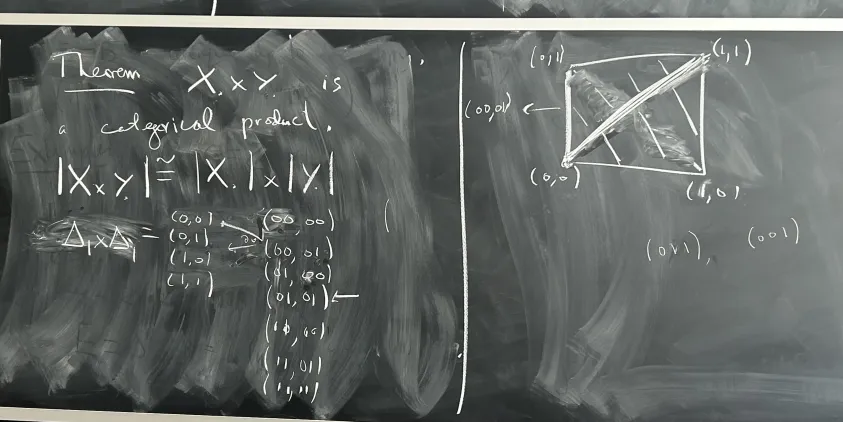
\includegraphics[width=0.6\textwidth]{Figures/sset_square.png}\]
    There is a discussion to be map on how the triangulation of the square is specified by the degeneracy maps, we will discuss this in more detail next time, though, in clearer details.
\end{example}

Given the geometric realization functor, we also define a functor going backwards.
\begin{definition}
    There is also a functor $\operatorname{Sing}: Space \to sSets$ (called the \textbf{singular simplicial set}) constructed as follows - for each $n$, we define
    \[\operatorname{Sing}_n(X) = \{\sigma: \Delta^n \to X\}\]
    as all the singular $n$-simplexes of $X$. The face maps are given by pre-composition with face maps of $\{\Delta^n\}_{n=0, 1,...}$ (note that they go the other direction).
    \[\partial_i \sigma \in \operatorname{Sing}_{n-1}(X), (\partial_i \sigma)(t \in \Delta^{n-1}) \coloneqq \sigma(\partial_i t)\]
    The degeneracy maps are given by pre-composition with degeneracy maps of $\{\Delta^n\}_{n=0, 1,...}$.
    \[s_i \sigma \in \operatorname{Sing}_{n+1}(X), (s_i \sigma)(t \in \Delta^{n+1}) \coloneqq \sigma(s_i t).\]
\end{definition}

We will note prove the following theorem, but we have the following two remarkable results.
\begin{theorem}
    $|\operatorname{Sing} X| \simeq X$. In fact, $|\bullet|$ is left adjoint to $\operatorname{Sing}(\bullet)$.
\end{theorem}

There is also a theorem of Kan, that we cannot state too precisely due to the limitations of this class, as follows.
\begin{theorem}[Kan]
    There is an equivalence between the homotopy theories of simplicial sets and that of topological spaces.
\end{theorem}

\begin{definition}
    A simplicial space of a functor $X: \Delta^{op} \to \operatorname{Space}$. In this case, there is still a geometric realization $|X|$ given by
    \[\bigsqcup_n X_n \times \Delta^n/\sim\]
    Here $X_n$ no longer has the discrete topology and instead have the natural topology it has as $X_n$ in spaces.
\end{definition}

\subsection{The Nerve of a Category}
For the remaining discussions in this lecture, we will introduce the notion of a topological category.

\begin{definition}
    A (small) \textbf{topological category} $\mathcal{C}$ is a category enriched over $\operatorname{Top}_*$ (ie. the entire collection $\operatorname{Ob}(\Ccal)$ and $\operatorname{Mor}_\Ccal(x, y)$ are topological spaces).
\end{definition}

From the topological category, we can define the notion of the \textbf{nerve of a category}.
\begin{definition}
    Let $\Ccal$ be any small category (does not have to be a topological category), the \ul{nerve of $\mathcal{C}$}, denoted $N\Ccal$ is a simplicial set
    \[N\Ccal_0 = \operatorname{Obj} \mathcal{C}, N \Ccal_1 = \bigsqcup_{x_0, x_1} \mathcal{C}(x_0, x_1),\]
    and in general $N \mathcal{C}_k$ composes of composable $k$-tuples $(\varphi_1, ..., \varphi_k)$. This means that, each $\varphi_i$ is a morphism in $\Ccal$, and the source of $\varphi_1$ is the target of $\varphi_2$, etc...\\
    
    The face and degeneracy maps are defined as follows. The degeneracy map $s_i: N \mathcal{C}_n \to N \mathcal{C}_{n+1}$ takes a sequence of $n$ composable maps
    \[c_0 \to c_1 \to ... \to c_n\]
    and it inserts an identity at $c_i$ maps in the $i$-th spot, ie. $s_i$ of the sequence above becomes
    \[c_0 \to c_1 \to ... \to c_i \to_{id} c_i \to c_{i+1} \to ... \to c_n.\]
    The face map $\partial_i: N \mathcal{C}_n \to N \mathcal{C}_{n-1}$ takes a sequence of $n$ composable maps
    \[c_0 \to c_1 \to ... \to c_i \to_{f_i} c_{i+1} \to_{f_{i+1}} ... \to c_n\]
    and just composes the $i$-th and $i+1$-th arrow for $0 < i < n$ (leaving out the first and last arrow). In other words, it becomes
    \[c_0 \to c_1 \to ... \to c_{i} \to_{f_{i+1} \circ f_i} c_{i+2} \to ... \to c_n. \]
    One can check that this indeed forms a simplicial set.
\end{definition}

\begin{remark}
    When $\Ccal$ is a topological category, we can define its nerve $N\Ccal$ to become a simplicial space (as opposed to a simplicial set).
\end{remark}

Here is an example that realizes the nerve of a category.
\begin{example}
    Let $X$ be a space, $\{U_\alpha\}$ a cover of $X$, the \textbf{\v{C}ech nerve} or the \textbf{nerve of an open cover} $\mathcal{C}^v_U$ is a simplicial space constructed as follows. As a remark, note that we use $\mathcal{C}^v_U$ to emphasize its correspondence to the underlying \v{C}ech cohomology. 
    \begin{itemize}
        \item $(\mathcal{C}^v_U)_0$ is the collection $\bigsqcup_\alpha U_{\alpha}$
        \item $(\mathcal{C}^v_U)_1$ is the collection $\bigsqcup_{\alpha, \beta} U_{\alpha \beta}$ (here $U_{\alpha \beta}$ are again $U_{\alpha} \cap U_{\beta}$).
        \item $(\mathcal{C}^v_U)_2$ is the collection $\bigsqcup_{\alpha, \beta, \gamma} U_{\alpha \beta \gamma}$
        \item And so on ... Here we write disjoint union to give them natural topologies.
    \end{itemize}
   Here the face maps are given by natural inclusions to parent spaces with less intersection. The degeneracy maps are given by inserting copies of indicies. For example, it would send $U_{\alpha \beta}$ to $U_{\alpha \beta \beta}$ (but note that the two spaces are the same as sets).
   %  Here $s: \bigsqcup U_{\alpha \beta} \to \bigsqcup U_{\alpha}$ is given by
   %  \[s(x \in U_{\alpha \beta}) = (x \in U_{\beta}), t(x \in U_{\alpha \beta}) = (x \in U_{\alpha}).\]
   %  If $x \in U_{\alpha \beta}, y \in U_{\gamma \delta}$, then 
   % \mattie{tbd}
\end{example}

We state the following fact but will not prove it.
\begin{theorem}[\v{C}ech Nerve Theorem]
    There is a homotopy equivalence $|C^v_{U}| \simeq X$, whenever there exists a partition of unity for the open cover $U$.
\end{theorem}

\begin{remark}
    The usual \v{C}ech nerve construction makes a simplicial set where each non-empty intersection is replaced by a point. In this case we do need the hypothesis that  $X$ is compact and the pairwise intersection of the $U_{\alpha}$'s are all contractible or empty, in order for the theorem to be true. However, in our case, since we are remembering them as spaces already, this is not needed.
\end{remark}

\begin{example}
    For the sake of sanity, we give the following example of the proposition. Here we take $[0,1]$ with a cover of two open sets given by $U$ and $V$. The lower diagram is the geometric realization of $C^v_U$.
    \[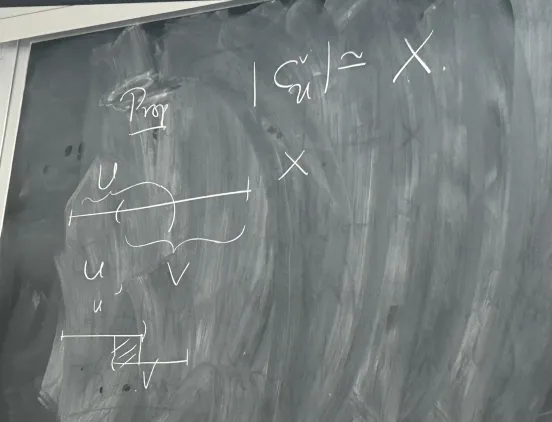
\includegraphics[width=0.5\textwidth]{Figures/cech_example.png}\]
\end{example}

\begin{definition}
    A functor $F: \Ccal \to \Dcal$ of topological categories is a \textbf{continuous functor} in the sense that its corresponding maps $\operatorname{Ob}(\Ccal) \to \operatorname{Ob}(\Dcal)$ is continuous, and $\operatorname{Mor}_{\Ccal}(x, y) \to \operatorname{Mor}_{\Dcal}(F(x), F(y))$ is continuous.
\end{definition}

\begin{proposition}
    Let $F: \Ccal \to \Dcal$ be a continuous functor, then we get a natural map $|F|: |N \mathcal{C}| \to |N \mathcal{D}|$. If $F_0, F_1: \Ccal \to \Dcal$ have a natural transformation between them, then $|F_0| \simeq |F_1|$ are homotopic maps.
\end{proposition}
    
\begin{proof}[Proof Sketch]
    To prove this, we let $\mathcal{I}$ be the small diagram category with two objects $0$ and $1$ and one non-identity morphism $0 \to 1$. We can check that
    \[|N\mathcal{I}| \cong [0,1].\]
    From here, we can check that a natural transformation from $F_0$ to $F_1$ is the same thing as a functor from the Cartesian product category $\mathcal{D}$:
    \[H: \mathcal{I} \times \mathcal{C} \to \mathcal{D}\]
    such that $H|_{0 \times \Ccal} = F_0$ and $H|_{1 \times \Ccal} = F_1$.\\

    From here, we can show that
    \[|H|: |N(\mathcal{I}) \times \mathcal{C}| = I \times |N \mathcal{C}| \to |N \mathcal{D}|\]
    is the desired homotopy between $|F_0|$ and $|F_1|$.
\end{proof}

\newpage
\section{Lecture October 29th, 2024}

There are a couple things we want to clear up from last time:
\begin{enumerate}
    \item We have a geometric realization functor $|\bullet|: \operatorname{sSet} \to T$ to our nice category of spaces. We made the following claim.
    \begin{theorem}
        The geometric realization functor commutes with Cartesian product, that is
        \[|X \times Y| \cong |X| \times_T |Y|.\]
    \end{theorem}
    Here, one should be careful that the Cartesian product on the RHS is taken in the category $T$, which is not always the usual Cartesian product topology in Top!!

    \item If $X$ is a topological space and $U = \{U_{\alpha}\}$ a cover, then we defined $C^{v}_{\bullet}(U)$ as the simplicial space where the zero simplices are $\bigsqcup_{\alpha \in A} U_{\alpha}$, the one simplices are $\bigsqcup_{\alpha, \beta \in A} U_{\alpha \beta}$, the two simplicies are $\bigsqcup_{\alpha, \beta, \gamma \in A} U_{\alpha \beta \gamma}$. The face maps are inclusions and the degeneracy maps are inclusions into intersections with degenerate indices.\\

    Then we made the claim that.
    \begin{theorem}[\v{C}ech Nerve Theorem]
        $|C^{v}_{\bullet} U| = \bigsqcup_p (\bigsqcup_{a_0, ..., a_p} U_{\alpha_0, ..., a_p}) \times \Delta^p/\sim$ is homotopy equivalent to $X$, whenever there exists a partition of unity for the open cover $U$.
    \end{theorem}
\end{enumerate}

\subsection{Topological Category}

To formally introduce our definition again, we will also clarify.
\begin{definition}
    A topological category consists of two spaces $\mathcal{O}$ (object) and $A$ (morphism), two functions $s,r : A \to \mathcal{O}$ (source and range/target), and a function $\circ: A \times_{\mathcal{O}} A \to A$ (composition). Here $A \times_{\mathcal{O}} A = \{(a, b) \in A \times A\ |\ s(a) = r(b)\}$ such that the following two conditions hold:\\

    1. (Composition is associative) We have that the following commutative diagram
    % https://q.uiver.app/#q=WzAsNCxbMCwwLCJBIFxcdGltZXNfTyBBIFxcdGltZXNfTyBBIl0sWzEsMCwiQSBcXHRpbWVzX08gQSJdLFsxLDEsIkEiXSxbMCwxLCJBIFxcdGltZXNfTyBBIl0sWzMsMiwiXFxjaXJjIiwyXSxbMSwyLCJcXGNpcmMiXSxbMCwzLCJwXzEiLDJdLFswLDEsInBfMiJdXQ==
\[\begin{tikzcd}
	{A \times_O A \times_O A} & {A \times_O A} \\
	{A \times_O A} & A
	\arrow["{p_2}", from=1-1, to=1-2]
	\arrow["{p_1}"', from=1-1, to=2-1]
	\arrow["\circ", from=1-2, to=2-2]
	\arrow["\circ"', from=2-1, to=2-2]
\end{tikzcd}\]
where $p_1(a_1, a_2, a_3) = (a_1, a_2 \circ a_3)$ and $p_2(a_1, a_2, a_3) = (a_1 \circ a_2, a_3)$.\\

2. (Composing with identity does not Change) We have another commutative diagram
% https://q.uiver.app/#q=WzAsOCxbMCwxLCJPIFxcdGltZXNfTyBBICJdLFsxLDEsIkEgXFx0aW1lc19PIEEiXSxbMiwxLCJBIl0sWzIsMiwiQSJdLFswLDIsIkEgXFx0aW1lc19PIE8iXSxbMSwyLCJBIFxcdGltZXNfTyBBIl0sWzAsMCwiXFx7KG8sIGEpfHIoYSk9b1xcfSJdLFswLDMsIlxceyhhLCBvKXxzKGEpPW9cXH0iXSxbMCwxXSxbNCw1XSxbNSwzLCJcXGNpcmMiXSxbMSwyLCJcXGNpcmMiXV0=
\[\begin{tikzcd}
	{\{(o, a)|r(a)=o\}} \\
	{O \times_O A } & {A \times_O A} & A \\
	{A \times_O O} & {A \times_O A} & A \\
	{\{(a, o)|s(a)=o\}}
	\arrow[from=2-1, to=2-2]
	\arrow["\circ", from=2-2, to=2-3]
	\arrow[from=3-1, to=3-2]
	\arrow["\circ", from=3-2, to=3-3]
\end{tikzcd}\]
Here the map $O \times_O A \to A \times_O A$ sends $(o, a)$ to $(id_o, a)$, and similarly for the other map.
\end{definition}

\begin{example}
    Here are some examples:
    \begin{enumerate}
        \item A topological monoid is a topological category with $1$-object.
        \item A topological group is a topologicalc ategory with $1$-object where every morphism is ``invertible".
        \item If $U = \{U_\alpha\}_\alpha$ is a cover of $X$, then there is a topological category $C^v(U)$ whose objects are $\mathcal{O} = \bigsqcup_{a \in A} U_a$ and $A = \bigsqcup_{a_0, a_1 \in A} U_{a_0 a_1}$. The source map $s: A \to \mathcal{O}$ is given by $(x \in U_{\alpha \beta}) \mapsto (x \in U_{\beta})$, the range map $r$ is given by $(x \in U_{\alpha \beta}) \mapsto (x \in U_{\alpha})$.\\

        In particular, $s(x \in U_{\alpha \beta}) = r(y \in U_{\gamma \delta})$ if and only if $\beta = \gamma$ and $x = y$. Thus the composition is given by
        \[(x \in U_{\alpha \beta}) \circ (x \in U_{\beta \gamma}) = (x \in U_{\alpha \gamma}).\]
        This is an example of a \textbf{topological groupoid}.
    \end{enumerate}
\end{example}

\begin{definition}
Given a topological category $\Ccal = (\mathcal{O}, A)$, we can define a \textbf{simplicial space, called the nerve of $\Ccal$,} as follows:
\begin{enumerate}
    \item $N \Ccal_0 = \mathcal{O}$
    \item $N \Ccal_1 = A$
    \item $N \Ccal_2 = A \times_O A$ is the pair of composable arrows.
    \item $N \Ccal_3 = A \times_O A \times_O A$
    \item and so on...
\end{enumerate}
In general $\partial_i: N C_{k} \to N C_{k-1}$ is given by sending $(a_1, ..., a_k)$ by composing the $i$-th term and the $i+1$-term in the sequence. ie. $\partial_1(a_1, ..., a_k) = (a_1 \circ a_2, a_3, ..., a_k)$, etc. $\partial_0$ knocks off the first term, and $\partial_k$ lnocks off the last term.\\

The degeneracy maps are given by $s_i: N \Ccal_{k-1} \to N \Ccal_{k}$ with $s_i(a_1, ..., a_{k-1}) = (a_1, ..., a_{i-1}, u(s(a_{i-1}), a_i, ..., a_{k-1})$. Here the map $u$ sends an object to its identity map.
\end{definition}

\subsection{Constructing $EG$ and $BG$}

Last time, we showed that if $F_0, F_1: \mathcal{C} \to \mathcal{D}$ are two continuous functors, then give rise to two functors
\[NF_0, NF_1: N \Ccal \to N \Dcal\]
Thus, we get two maps between their geometric realizations
\[B F_0, B F_1: |N \Ccal| \to |N \Dcal|.\]

\begin{remark}
    $|N \Ccal|$ is often also denoted $B \Ccal$, which is called \textbf{the classifying space of the topological category $\Ccal$}.
\end{remark}

Recall that if $N: F_0 \to F_1$ is a natural transformation, then this gives rise to a homotopy between
\[BN: B F_0 \to B F_1\]
Here the two maps go from $B \Ccal \to B \Dcal$. (Thus, $BN$ is concretely a function of the form $B \Ccal \times [0, 1] \to B \Dcal$).\\

To recall why this is the case, a natural transformation from $F_0$ to $F_1$ is really the same thing as a function from $\Ccal \times \mathcal{A} \to \Dcal$. Here $\mathcal{A}$ is a topological category with $(O, A)$ where $O = \{0, 1\}$ and $A = \{id_0, id_1, 0 \to 1 \}$. One can check that $|N \mathcal{A}| \cong [0, 1]$. Thus
\[|N(\Ccal \times \mathcal{A})| \cong |N\Ccal| \times_T |N \mathcal{A}| = |N \Ccal| \times_T [0, 1]\]
such that
\[H|_{\Ccal \times \{0\}} = F_0 \text{ and } H|_{\Ccal \times \{1\}} = F_1.\]


\begin{example}
Here are some examples:
\begin{enumerate}
    \item Let $U$ be an open cover of $X$, then $N C^{v}(U)$ (the Nerve of the topological category $C^{v}(U)$), then this is the name as $C^{v}_{\bullet}(U)$ is the \v{C}ech nerve.

    \item Let $X$ be a topological space, we can define $\Ccal$ whose objects are $X$ and whose morphisms are $X \times X$. The source and range maps are the projections to the first and second coordinates respectively. Here we have a composition between $(x, y)$ and $(z, w)$ if and only if $y = z$, and in this case
    \[(x, y) \circ (y, w) = (x, w).\]
    We can build a nerve by specifying $X \times X \times X = (X \times X) x_X (X \times X)$, and so on ...

    \begin{lemma}
        $B \Ccal$ in this example is contractible.
    \end{lemma}

    \begin{proof}
        Let $*$ be the category with one object and one morphism (think of this as a point). Let $\Ccal$ be the topological category in this particular example.\\
        
        Pick $x_0 \in X$, define a functor $F_{x_0}: * \to \mathcal{C}$ where $F_{x_0}(*) \equiv x_0$ and $F_{x_0}(id_*) = id_{x_0}$.\\

        From here we define a functor $G: \Ccal \to *$ where $G(x \in X) = *$ and $G(x, y) = 1_*$.\\

        Then $G \circ F_{x_0}$ is the identity functor on $*$. In particular, \ul{$B(G \circ F)$ is homotopic to the identity map on $B*$, which is a point.}\\

        On the other hand, $F_{x_0}  \circ G: \Ccal \to \Ccal$ such that
        \[F_{x_0} \circ G(x) = x_0 \text{ and } F \circ G(x, y) = (x_0, x_0).\]
        There is a natural transformation $F \circ G \to id_{\Ccal}$ (to the identity functor) as follows:
        \[\forall x \in X, N_x: F \circ G(x) = x_0 \to id_{\Ccal}(x) = x\]
        is the unique map from $x_0 \to x$ in the category. Thus, we also have that $F \circ G \simeq id_{\Ccal}$, and thus
        \[B(F \circ G) \simeq id_{B \Ccal}.\]

        Thus, we conclude that $B \Ccal$ is contractible!
    \end{proof}
\end{enumerate} 
\end{example}

\begin{definition}
Let $G$ be a Lie group, let $\mathcal{E} G$ be the topological category $G \times G \to G$ in the previous example (here this just uses the structure of $G$ as a topological space).\\

We let $BG$ e the topological category with one object (diagrammatically this is something like $\{G \rightrightarrows *\}$).
\end{definition}

From our previous discussion, we know that $|N \mathcal{E} G| \simeq \text{pt}$. On the other hand what is $N BG$?\\

Well, the face maps $\partial_2, \partial_1, \partial_0$ from $G \tiems G$ to $G$ take $(g_1, g_2)$ to $g_2, g_1 g_2, g_1$ respectively. The degeneracy map backwards send $g$ to $(g, e)$ or $(e, g)$.\\

More generally, the map is $NBG_k = G^k \to G^{k-1} = NBG_{k-1}$ is given by
\begin{align*}
    (g_1, ..., g_k) &\mapsto (g_2, ..., g_k)\\
    & \vdots\\
    &\mapsto (g_1, ..., g_i g_{i+1}, ..., g_k)\\
    &\vdots\\
    & \mapsto (g_1, ..., g_{k-1})
\end{align*}

Now $G$ has an action on $N \mathcal{E} G$ freely and properly discontinuous, such that - when we quotient out this $G$-action, we have a map that is an isomorphism
\[(N \mathcal{E} G)/G \to N B G\]

\begin{exercise}[Homework Problem]
    Figure out which action of $G$ gives this action.
\end{exercise}

Thus, this gives a principal $G$-bundle structure when taking geometric realization
\[|N \mathcal{E} G| \to |N BG|\]

\begin{definition}
    We call $EG = |N \mathcal{E} G|$ and $BG = |NBG|$.
\end{definition}

\begin{remark}
    This is sometimes more generally a process called the Bar construction, where we could choose a different $G$ action that is free and properly discontinuous.
\end{remark}

\begin{theorem}
    $EG \to BG$ is the universal principal $G$-bundle.
\end{theorem}

The advantage of this construction is that it is completely functorial. A homomorphism between Lie groups will give a corresponding map between their universal principal $G$-bundles.

\begin{proof}
    By the recognition principle and our previous discussions, this is evidently true. 
\end{proof}

We still need to prove the recognition principle, however. This will be done in the next lecture. For now, we seek to investigate the following.

\subsection{Cohomology of an Open Cover in Principal $G$-Bundles}
First we establish a technical lemma.

\begin{lemma}\label{lem::g_prin_coh_well_def}
Given $\pi: P \to B$ a principal $G$-bundle and a trivializing cover $U = \{U_\alpha\}_{\alpha \in A}$. Moreover, there is an isomorphism $\varphi_{\alpha}: P|_{U_\alpha} \to U_{\alpha} \times G$ that commutes in the definition of the bundle, which induces maps
\[g_{\alpha \beta}: U_{\alpha \beta} \to G, g_{\alpha \beta} \circ g_{\beta \gamma} = g_{\alpha \gamma}.\]

If $\varphi'_{\alpha}: P|_{U_{\alpha}} \to U_{\alpha} \times G$ is a different trivialization (but for the same cover), then in this case we get $g'_{\alpha \beta}$'s.\\

Then there exists $\psi: U_{\alpha} \to G$ such that
\[g_{\alpha \beta} = \psi_\alpha g'_{\alpha \beta}  \psi_{\beta}^{-1}.\]
\ul{\textbf{Here we should be careful that we do not mean compositions, but rather as product of elements in the group $G$.}}
\end{lemma}

\begin{proof}
    We have maps
    % https://q.uiver.app/#q=WzAsMyxbMCwwLCJQfF97VV9cXGFscGhhfSJdLFsxLDAsIlVfXFxhbHBoYSBcXHRpbWVzIEciXSxbMSwxLCJVX1xcYWxwaGEgXFx0aW1lcyBHIl0sWzAsMSwiXFx2YXJwaGlfXFxhbHBoYSJdLFswLDIsIlxcdmFycGhpX1xcYWxwaGEnIiwyXV0=
\[\begin{tikzcd}
	{P|_{U_\alpha}} & {U_\alpha \times G} \\
	& {U_\alpha \times G}
	\arrow["{\varphi_\alpha}", from=1-1, to=1-2]
	\arrow["{\varphi_\alpha'}"', from=1-1, to=2-2]
\end{tikzcd}\]
We observe that the identity map $1: P|_{U_\alpha} \to P|_{U_\alpha}$ is an isomorphism of the trivial principal bundle - specifically, the following diagram commutes:
% https://q.uiver.app/#q=WzAsNCxbMCwwLCJQfF97VV9cXGFscGhhfSJdLFsxLDAsIlVfXFxhbHBoYSBcXHRpbWVzIEciXSxbMSwxLCJVX1xcYWxwaGEgXFx0aW1lcyBHIl0sWzAsMSwiUHxfe1VfXFxhbHBoYX0iXSxbMCwxLCJcXHZhcnBoaV9cXGFscGhhIl0sWzAsMywiMSIsMl0sWzMsMiwiXFx2YXJwaGlfXFxhbHBoYSciLDJdLFsxLDJdXQ==
\[\begin{tikzcd}
	{P|_{U_\alpha}} & {U_\alpha \times G} \\
	{P|_{U_\alpha}} & {U_\alpha \times G}
	\arrow["{\varphi_\alpha}", from=1-1, to=1-2]
	\arrow["1"', from=1-1, to=2-1]
	\arrow[from=1-2, to=2-2]
	\arrow["{\varphi_\alpha'}"', from=2-1, to=2-2]
\end{tikzcd}.\]
In particular, if we look at the map $\varphi_{\alpha} \circ (\varphi'_{\alpha})^{-1}: U_a \times G \to U_a \times G$, it will be a map of the form
\[\varphi_{\alpha} \circ (\varphi'_{\alpha})^{-1}(x, g) = (x, \psi_{\alpha}(x) \cdot g).\]
Here $\psi_{\alpha}(x) \in G$ is some element dependent only on what $x \in U_\alpha$ is. This independence holds because what $(\varphi'_\alpha)^{-1}$ and $\varphi_\alpha$ does to the second coordinates are independent of $g \in G$. In particular, $\psi_{\alpha}$ outlines a map $U_\alpha \to G$, and we claim that this is our desired map.\\

% Thus, $\psi_{\alpha} \coloneqq \varphi_{\alpha} \circ (\varphi'_{\alpha})^{-1}$ is a map from $U_{\alpha} \to G$.\\

From here, we can check that that $g_{\alpha \beta} = \psi_{\alpha} g'_{\alpha \beta} \psi_{\beta}^{-1}$. Indeed, we note that $\psi_{\alpha} g'_{\alpha \beta} \psi_{\beta}^{-1}$ corresponds to the map $\varphi_{\alpha} \circ (\varphi_{\alpha}')^{-1} \circ (\varphi_{\alpha}' \circ \varphi_\beta'^{-1}) \circ ((\varphi_\beta') \circ \varphi_\beta^{-1}) = \varphi_\alpha \circ \varphi_\beta^{-1}$, which corresponds back to $g_{\alpha \beta}$.
\end{proof}

\begin{definition}
Independent of the bundle on $X$. We consider the following. Let $U = \{U_{\alpha}\}_{\alpha \in A}$ be an open cover of $X$. Recall a system of transition maps associated to $U$ is given by the collection $\{g_{\alpha \beta}: U_{\alpha \beta} \to G\}$ where:
\begin{enumerate}
    \item $g_{\alpha \beta}$ is continuous.
    \item (Identity Condition) $g_{\alpha \alpha}$ is the identity.
    \item (Cocycle Condition) $g_{\alpha \beta} \circ g_{\beta \gamma} = g_{\alpha \gamma}$.
\end{enumerate}
(These transition maps can always build a principal $G$-bundle). We let $C^1(U; G)$ be the collection of all possible systems of transition maps.\\

We say that two systems $\{g_{\alpha \beta}\} \sim \{g'_{\alpha \beta}\}$ if there exists a collection $\{\psi_\alpha: U_{\alpha} \to G\}$ such that for all indices,
\[g_{\alpha \beta} = \psi_\alpha g'_{\alpha \beta} \psi_{\beta}^{-1}.\]
\end{definition}

$C^1(U;G)$ are thought of as the $1$-cochains, from here we define a ``cohomology" as follows.

\begin{definition}
    We define $H^1(U; G)$ as $C^1(U;G)/\sim$. Note this is a pointed set with the ``base point corresponding to the trivial bundle". Explicitly the base point is the equivalence class of the trivial transition maps, ie. $g_{\alpha \beta}: U_{\alpha \beta} \to G$ is the constant map onto the identity.
\end{definition}

\begin{remark}
    If $G$ is abelian, then $H^1(U;G)$ may be given a group structure. However, when $G$ is not abelian, $H^1(U; G)$ is in general only a pointed set.
\end{remark}

We have defined the notion of a ``first cohomology" with respect one open cover of $X$. Now we want to give a first cohomology that is independent of the cover. $H^1(U; G)$ itself, however, is not independent of $U$, so we want some uniform object that combines the information given by all open covers. This leads to our consideration of colimits.

\begin{definition}
    A \textbf{refinement} of $U = \{U_\alpha\}_{\alpha \in A}$ is a cover $V = \{V_\beta\}_{\beta \in B}$ and a map $\psi: B \to A$ such that
    \[\forall \beta \in B, V_\beta \subseteq U_{\psi(\beta)}.\]
\end{definition}

\begin{definition}
    Given $U$ and a refinement $V$, there exists a \textbf{natural restriction map}
    \[\operatorname{res}_{UV}: H^1(U; G) \to H^1(V; G)\]
    defined as follows - for each (equivalence class of) transition maps $\{g_{\alpha \beta}: U_{\alpha \beta} \to G\}$, we can product transition maps $\{h_{\gamma \delta}: V_{\gamma \delta} \to G\}$ by specifying that 
    \[h_{\gamma \delta}: V_{\gamma \delta} \subseteq U_{\psi(\gamma) \psi(\delta)} \text{ is the restriction of } g_{\psi(\gamma) \psi(\delta)}.\]
    We define $H^1(X; G)$ as the colimit of the $H^1(U; G)$'s over these refinements of all open cover of $G$.
\end{definition}

\begin{remark}
   $H^1(X; G)$ may be defined alternatively in the language of sheaf cohomology. Let $\mathcal{F}$ be a sheaf of groups on $X$, and for each open set $U$ of $X$, $\mathcal{F}(U)$ is the group of continuous functions from $U$ to $G$. In this case, $H^1(X; G)$ is exactly the 1st sheaf cohomology with respect to $\mathcal{F}$. (There is a subtlety in what we mean by sheaf cohomology if the group is not abelian, but the general construction will align). $H^1(X; G)$ is not typically the singular cohomology, despite the notation. However, if $G$ is discrete, then $\mathcal{F}$ is the sheaf of locally constant maps with values in $G$, and $H^1(X; G)$ agrees with the singular cohomology in $G$.
\end{remark}

\begin{theorem}
    When $X$ is paracompact, there is an isomorphism $H^1(X; G) \cong P_G(X)$ between the first cohomology (again, this should not be confused with the singular case) and isomorphism classes of principal $G$-bundles.
\end{theorem}

\begin{remark}
    There is an equivalent formulation of the statement specifying that $P_G(X)$ are in bijection with homotopy classes of maps $[X, BG]$. In the case that $G$ is discrete, $BG = K(G, 1)$, and we know that $[X, K(G, 1)]$ is the ordinary singular cohomology in $G$-coefficients.
\end{remark}

We might come back and formally prove this, but for now we give a proof sketch.

\begin{proof}[Proof Sketch]
    For each $H^1(U; G)$, given an equivalence class of transition maps $\{g_{\alpha \beta}\}$ on $X$, we can construct a principal bundle $P \to X$ whose isomorphism class is well-defined up to equivalence (perhaps using Lemma~\ref{lem::g_prin_coh_well_def}). Furthermore, one can check that these maps commute with restrictions. Thus, we have a collection of maps $f_U: H^1(U; G) \to P_G(X)$. The universal property of colimits then gives us a map $H^1(X; G) \to P_G(X)$, which one can check to be an isomorphism.

   %  To check that $P_G(X)$ is isomorphic to $H^1(X; G)$, it suffices for us to check that $P_G(X)$ and the collection $\{f_U\}$ satisfies the universal property of the colimit. Now, suppose we have a collection of maps $\Tilde{f}_U: H^1(U; G) \to A$ that are compatible to transitio maps, then we specify a map $P_G(X) \to A$

    
   % Let $P \to X$ be a principal $G$-bundle,  Lemma~\ref{lem::g_prin_coh_well_def} guarantees that the element representing $P \to X$ in $H^1(U; G)$ is independent of the choice of trivialization on $P \to X$ for the same cover. Thus, $(P \to X)$ gives a well-defined element in $H^1(U; G)$.\\

   % This induces a map $P_G(X) \to H^1(U; G)$ for all open cover $U$ that commutes with the restriction maps. 
\end{proof}

\begin{example}
Suppose $P \to X$ is a principal $G$-bundle. Let $U = \{U_\alpha\}$ be a cover, $g_{\alpha \beta}: U_{\alpha \beta} \to G$ be the transition functions. From here we consider the \v{C}ech nerve $C^{v}(U)$ and $NBG$. Let us compare them:
\[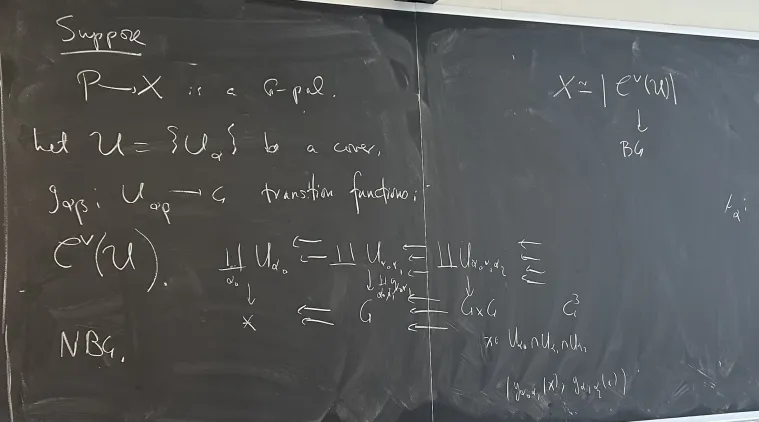
\includegraphics[width=0.8\textwidth]{Figures/NBG_Cech.png}\]
Note that these vertical morphisms commute with their internal simplicial and degeneracy maps exactly because of a \textbf{cocycle conditions}!\\

Taking this over to its geometric realization, we obtain an explicit map
\[X \simeq  |C^{v}(U)| \to BG.\]
In this case, the pullback of $EG \to BG$ along this map gives a bundle equivalent to $P \to X$.
\end{example}

\begin{remark}
    There are more explicit constructions of maps from $X \to BG$ in specialized cases (ex. the Gauss map).
\end{remark}

\newpage
\section{Lecture October 31st, 2024}

We haven't proven the essential punchline on how homotopy results have anything to do with principal $G$-bundles. This is the goal of our lecture today. We state the result as follows.

\subsection{Homotopy Invariance of Pullback of Principal G-bundles}

\begin{theorem}\label{thm::homotopy_inv_pullback_bundle}
    Let $\pi: P \to X$ is a principal $G$-bundle and $Y$ be a CW complex, and $f_0, f_1: Y \to X$ are homotopy maps, then the pullbacks $f_0^+ P$ and $f_1^* P$ are isomorphic as principal $G$-bundles.
\end{theorem}

\begin{remark}
    The theorem is true generally for any $(G, F)$-fiber bundles, and in particular it will apply to vector bundles. The proof should be fairly similar too.
\end{remark}

We make a couple comments/facts before proving this - let $P \to X$ be a principal $G$-bundle\\

1. Suppose $F$ is a left $G$-space, then we can form an associated bundle $P \times_G F \to X$, which we recall is
    \[P \times_G F = P \times F/\sim, (pg, f) \sim (p, gf)\]
 Note that this equivalence relation is the same as stating that $(pg, g^{-1} f) \sim (p, f)$.\\

2. We will state and prove the following lemma:
    \begin{lemma}
        Consider the associated bundle $P \times_G F \to X$, then we can compute its sections as follows:
        \[\Gamma(X; P \times_G F) \cong \{\varphi: P \to F\ |\ \varphi(pg) = \varphi(p) \cdot g\}\]
        (ie. it is the collection of right $G$-equivariant functions from $P \to G$.) Note that here $F$ is a left $G$-space by hypothesis, and we give a right $G$-space structure on $F$ by specifying an action that
        \[f \cdot_{right} g \coloneqq = g^{-1} \cdot_{left} f.\]
        Under this interpretation, the sections may also be computed as
        \[\Gamma(X; P \times_G F) \cong \{\varphi: P \to F\ |\ \varphi(pg) = g^{-1} \cdot \varphi(p)\}\]
    \end{lemma}

\begin{example}
    If $G$ acts \textbf{on the right} of $P$, then consider $C^0(P)$ is collection of contnuous $\Cbb$-valued functions on $P$. Then $G$ acts \textbf{on the left} of $C^0(P)$ given by
    \[g \cdot f(p) \coloneqq f(p \cdot g).\]
    We can check this is a valid action because
    \begin{align*}
       f(p g_1 g_2) &= (g_1 g_2)f(p)\\
       &= g_1(g_2 f(p))\\
       &= (g_2 f)(p g_1)\\
       &= f((pg_1) g_2)\\
       &= f(p g_1 g_2).
    \end{align*}
\end{example}

\begin{proof}[Proof of Lemma]
    Let $\varphi \in \{\varphi: P \to F\ |\ \varphi(pg) = \varphi(p) \cdot g\}$, we specify a map $s_{\varphi}(x)$ for $x \in X$ to be given by 
    \[s_\varphi(x) = (p, \varphi(p)) \in P \times_G F,\]
    where $p$ is any lift of $x$ to $P$ (we just mean $p$ is in the fiber of $x$).  Note that if we lifted to any other fiber $p'$, then there exists a unique $g \in G$ such that $p' = pg$. Thus, 
    \[(p', \varphi(p')) = (pg \varphi(p)g) = (pg, g^{-1} \varphi(p)) \sim (p, \varphi(p)).\]
    Thus, our map is well-defined.\\

    Conversely, let $s \in \Gamma(X, P \times_G F)$, then we define $\varphi_s: P \to F$ as follows - for $p \in P$ and let $\pi: P \times_F G \to X$, then we have an element $s(\pi(p)) \in P \times_G F$. Because this is the associated bundle of a principal $G$-bundle, we can choose a representative of $s(\pi(p))$ of the form $(p, f_p)$, where $f_p \in F$ depends on $p$. From here, we specify
    \[\varphi_s(p) = f_p.\]

    One can check that these two maps are inverses of each other.
\end{proof}

Now we are ready to prove the theorem.

\begin{proof}[Proof of Theorem~\ref{thm::homotopy_inv_pullback_bundle}]
    Let $F: Y \times I \to X$ be a homotopy between $f_0 \simeq f_1: Y \to X$. We consider the pullback $F^*(P) \to Y \times I$. The theorem then follows from the lemma:

    \begin{lemma}
        Let $\pi: Q \to Y \times I$ be a $G$-principal bundle, $Q_0 = Q|_{Y \times \{0\}}$, then $Q$ is isomorphic to $Q_0 \times I$.
    \end{lemma}

    \begin{proof}[Proof of Lemma]
        Recall that a morphism between principal $G$-bundles is an isomorphism. Thus, it suffices for us to construct a morphism $Q \to Q_0 \times I$. By the previous lemma before this, we just need to show that there exists a section of the form
        \[Q \times_G (Q_0 \times I) \to Y \times I.\]
        But we already have a section $s_0$ to this map above corresponding to $1_{Q_0}: Q_0 \to Q_0$, this is because of the following sub-lemma:

        \begin{lemma}
            If $\pi: Z \to Y \times I$, where $Y$ is a CW-complex, is a Serre fibration, and we have a section $s_0: Y \times \{0\} \to Z$, then there exists an extension $s: Y \times I \to Z$ that is also a section.
        \end{lemma}

        \begin{proof}[Proof of Sub-Lemma]
            This comes from solving the lifting problem
            % https://q.uiver.app/#q=WzAsNCxbMCwwLCJZIFxcdGltZXMgXFx7MFxcfSJdLFswLDEsIlkgXFx0aW1lcyBbMCwgMV0iXSxbMSwwLCJaIl0sWzEsMSwiWSBcXHRpbWVzIEkiXSxbMCwxLCIiLDAseyJzdHlsZSI6eyJ0YWlsIjp7Im5hbWUiOiJob29rIiwic2lkZSI6InRvcCJ9fX1dLFswLDIsInNfMCJdLFsxLDMsIjEiXSxbMiwzXSxbMSwyLCJzIiwxLHsic3R5bGUiOnsiYm9keSI6eyJuYW1lIjoiZGFzaGVkIn19fV1d
\[\begin{tikzcd}
	{Y \times \{0\}} & Z \\
	{Y \times [0, 1]} & {Y \times I}
	\arrow["{s_0}", from=1-1, to=1-2]
	\arrow[hook, from=1-1, to=2-1]
	\arrow[from=1-2, to=2-2]
	\arrow["s"{description}, dashed, from=2-1, to=1-2]
	\arrow["1", from=2-1, to=2-2]
\end{tikzcd}\]
        \end{proof}

        Thus, we can extend this to $s: Y \times I \to Q \times_G (Q_0 \times I)$, which corresponds to a morphism $Q \to Q \times I$.
    \end{proof}

\end{proof}

    \begin{corollary}
        If $X$ is contractible, then every princiapl $G$-bundle is isomorphic to $X \times G$.
    \end{corollary}

\subsection{Homotopy Classification of Principal $G$-bundles}
    \begin{theorem}
        Let $\pi: P \to B$ be a principal $G$-bundle, suppose $P$ is weakly  contractible, then for all CW complexes, the map
        \[\alpha: [X, B] \to P_G(X)\]
        by sending $\varphi: X \to B$ to $\varphi^*(B) \to X$, is an isomorphism of sets.
    \end{theorem}

    \begin{proof}
        Suppose $P$ is weakly contractible:
        \begin{enumerate}
            \item \textbf{$\alpha$ is surjective:} Let $Q \to X$ be a principal $G$-bundle, then $Q \times_G P \to P$ has $P$ as a fiber, which is weakly contractible, so there is a general fact \textbf{which will be on your homework} that implies that we have a section.\\

            By our identiciation of sections and $G$-equivariant maps, there then exists a $G$-equivariant map $\Phi: Q \to P$. Let $\varphi: X \to B$ be the induced map on quotient, ie.
            % https://q.uiver.app/#q=WzAsNCxbMCwwLCJRIl0sWzEsMCwiUCJdLFswLDEsIlgiXSxbMSwxLCJCIl0sWzAsMl0sWzAsMSwiXFxQaGkiXSxbMSwzXSxbMiwzLCJcXHZhcnBoaSJdXQ==
\[\begin{tikzcd}
	Q & P \\
	X & B
	\arrow["\Phi", from=1-1, to=1-2]
	\arrow[from=1-1, to=2-1]
	\arrow[from=1-2, to=2-2]
	\arrow["\varphi", from=2-1, to=2-2]
\end{tikzcd}\]
Note that this square is a pullback, and we automatically have that $Q \cong \varphi^*(P)$.

    \item $\alpha$ is injective: Suppose $f_0, f_1: X \to B$ such that $f^*_0 P \cong f_1^* P$. Let $\psi$ be the isomorphism between the two pullback bundles.  Let $Q \to X \times I$ be the principal $G$-bundle $(f_0^* P) \times I$. Consider the associated bundle
    \[\tau: Q \times_G P \to X \times I.\]
    We have equivariant maps $Q_0 = f^*_0 P \to P$, and $Q_1 = f_1^*(P) \cong f_0^*(P) \to P$.

    These maps correspond to section of $\tau$ over $X \times \{0\}$ and $X \times \{1\}$. Since the fiber $P$ is weakly contractible, there exists a section $s$ over $X \times I$ extending it, so there exists a principal $G$-bundle $Q \to P$. Now we can pass this to the quotient.
        \end{enumerate}
    \end{proof}

\begin{corollary}
    If $P \to B$ is a principal $G$-bundle, and $P$ is weakly contractible, then $P \to B$ is the universal $G$-bundle, over the CW complexes.
\end{corollary}

\begin{corollary}
Let $H \subseteq G$ be a closed sub-Lie group of $G$, if $P \to B = P/G$ is a universal $G$-bundle, then $P \to P/H$ is the universal $H$-bundle.    
\end{corollary}

\begin{proof}
    This follows from the previous corollary because $P \to P/H$ is a principal $H$-bundle (as $H$ is a closed sub-Lie group) and $P$ is weakly contractible.
\end{proof}

\subsection{Inducing and Reducing Bundles}

We make the following remark without proof.
\begin{proposition}\label{BG_closed_incl}
If $\alpha: H \to G$ is a homomorphism of Lie groups, then our functorial construction of classfying spaces gives us a map $B \alpha: BH \to BG$. In the specific case where $H \to G$ is a closed inclusion, $B \alpha$ is exactly the map $P/H \to P/G$, whose fiber is $G/H$.    
\end{proposition}


\begin{definition}[Induced Bundles]
    If $\alpha: H \to G$ is a homomorphism of Lie groups, and clearly $H$ has an action on $G$. Let $\pi: Q \to X$ be a principal $H$-bundle, then $Q \times_H G \to X$ is a principal $G$-bundle, which we call the \textbf{induced principal $G$-bundle}. 
\end{definition}

\begin{definition}[Reducing Bundles]
    If $\alpha: H \to G$ is a homomorphism of Lie groups. Given a principal $G$-bundle $P \to X$, we say that the structure group $G$ reduces to $H$, if there exists a principal $H$-bundle $Q \to X$ such that $P \cong Q \times_H G$. 
\end{definition}

\begin{remark}
    If $P$ has a trivializing cover $U = \{U_\alpha\}$ and transition functions $g_{\alpha\beta}: U_{\alpha \beta} \to G$, \textbf{a reduction of $G$ to $H$} is the existence of transition functions $h_{\alpha \beta}: U_{\alpha \beta} \to H$ (you might have to choose a finer cover), such that $\{g_{\alpha \beta}\} \sim \{\alpha(h_{\alpha \beta})\}$. Here $\alpha$ is the fixed group homomorphism $H \to G$, and $\sim$ is the equivalence relation defined last lecture.
\end{remark}

Here are some examples of this theory.
\begin{example}
    Let $P \to X$ be a principal $\operatorname{GL}_n(\Rbb)$-bundle, then a reduction of $P$ to $GL_n(\Rbb)^+ = \{g\ |\ \operatorname{det}(g) > 0\}$ is the same as giving an orientation.\\
    
    To be more precise, let $E = P \times_{GL_n(\Rbb)} \Rbb^n$ be the associated bundle to $P$, note that $E$ is a real-vector bundle. Let $F' = P' \times_{GL_n(\Rbb)'} \Rbb^n$, where $P'$ is a reduction of $P$ to $\operatorname{GL}_{n}(\Rbb)^+$. Then $E'$ is the choice of $E$ with an orientation (in the sens eof a real vector bundle).
\end{example}

\begin{example}
    If we reduce to $O(n) \subseteq \operatorname{GL}_n(\Rbb)$ instead, then $E' \cong P' \times_{O(n)} \times \Rbb^n$ is a vector bundle with a chosen inner product. If we reduce to $SO(n) \subseteq \operatorname{GL}_n(\Rbb)$, then $E' \cong P' \times_{SO(n)} \times \Rbb^n$ is an oriented vector bundle with a chosen inner product.
\end{example}

\begin{example}
    $GL_n(\Cbb)$ sits inside $\operatorname{GL}_{2n}(\Rbb)^+$ (complex matrices are always orientation persevering). In this case, reducing a $\operatorname{GL}_{2n}(\Rbb)$-bundle to $\operatorname{GL}_n(\Cbb)$ is equivalent to taking a rank $2n$-real vector bundle and giving it with a complex rank $n$ vector bundle structure.
\end{example}

\begin{remark}
    Apparently, you could even get a foliation for reducing to a nice group.
\end{remark}

\subsection{Sympletic Manifolds and Spin Groups}

\begin{definition}
    A sympletic manifold $(M, \omega)$ is a smooth manifold together with a closed real $2$-form $\omega \in \Omega^2(M)$ which is non-degenerate (ie. $\omega: \Lambda^2 TX \to \Rbb$, $\omega(c, \eta) = 0$ for all $\eta$ implies that $c = 0$).\\

    When we have a vector space $V$ and a sympletic form $\omega$ on it, we can define the sympletic group as
    \[\operatorname{Sp}(V, \omega) = \{A \in \operatorname{GL}(v)\ |\ \omega(Av, Au) = \omega(v, u)\} \subseteq \operatorname{GL}(V).\]
\end{definition}

\begin{remark}
    A Riemannian manifold is a smooth manifold equipped with a \textbf{symmetric $2$-tensor}! A sympletic manifold is a smooth manifold equipped with a (closed) \textbf{anti-symmetric $2$-tensor}!
\end{remark}

\begin{definition}
    For $n \geq 3$, we know that $\pi_1(\operatorname{SO}(n)) = \Zbb/2\Zbb$. From covering space theory there is a two-sheeted universal covering of $\operatorname{SO}(n)$ called the \textbf{Spin group} $\operatorname{Spin}(n)$. Diagrammatically, we have that
    \[\Zbb/2 \to \operatorname{Spin}(n) \to_{\alpha} \operatorname{SO}(n).\]
\end{definition}

\begin{example}
    $\Rbb^{2n}$ with $\omega = \sum_{i=1}^n dx^i \wedge dy^i$ is a symmpletic manifold!
\end{example}

\begin{theorem}[Darboux's Theorem] Given $(M, \omega)$ a symmpletic manifold and let $x \in M$, then there exists a local chart $U$ such that $\omega = \sum dx^i \wedge dy^i$.
\end{theorem}

\begin{remark}
    In particular, Darboux's Theorem implies that we don't have any local invariants in sympletic geometry! This is a stark contrast to Riemannian geometry, where curvature is a canonical example of local invariants.
\end{remark}

Now we derive a criterion for when a principal $G$-bundle can be reduced.
\begin{theorem}
    Let $\pi: P \to X$ be a prinicipal $G$-bundle and $\alpha: H \to G$ be a group homomorphism, then the following are equivalent:
    \begin{enumerate}
        \item $P$ can be reduced to $H$.
        \item $P \times_G (G/H) \to X$ has a section.
        \item Let $f$ be defined in the left diagram, then it has a lift in the right diagram: % https://q.uiver.app/#q=WzAsNyxbMCwwLCJQIl0sWzAsMSwiWCJdLFsxLDEsIkJHIl0sWzEsMCwiRUciXSxbMywwLCJCSCJdLFszLDEsIkJHIl0sWzIsMSwiWCJdLFswLDEsIlxccGkiLDJdLFszLDIsIlxccGkiXSxbMSwyLCJmIiwyXSxbMCwzXSxbNCw1LCJCXFxhbHBoYSJdLFs2LDUsImYiLDJdLFs2LDQsIlxcVGlsZGV7Zn0iLDAseyJzdHlsZSI6eyJib2R5Ijp7Im5hbWUiOiJkYXNoZWQifX19XV0=
\[\begin{tikzcd}
	P & EG && BH \\
	X & BG & X & BG
	\arrow[from=1-1, to=1-2]
	\arrow["\pi"', from=1-1, to=2-1]
	\arrow["\pi", from=1-2, to=2-2]
	\arrow["{B\alpha}", from=1-4, to=2-4]
	\arrow["f"', from=2-1, to=2-2]
	\arrow["{\Tilde{f}}", dashed, from=2-3, to=1-4]
	\arrow["f"', from=2-3, to=2-4]
\end{tikzcd}\]
    \end{enumerate}
\end{theorem}

\begin{proof}
 For (1) implies (2): If $P = Q \times_H G$, then $P \times_G (G/H) = (G \times_H G) \times_G G/H$. One can check that there is a homeomorphism from this to
 \[Q \times_H (G/H).\]
 The coset $eH$ is a fixed point for the $H$-action on $G/H$, so there is an $H$-equivariant map that sends a point $* \to G/H$ by sending $* \to eH$. In this case, this induces a map
 \[Q \times_H * \to Q \times_H G/H\]
 % https://q.uiver.app/#q=WzAsMyxbMCwwLCJRIFxcdGltZXNfSCAqIl0sWzAsMSwiWCJdLFsxLDAsIlEgXFx0aW1lc19IIEcvSCJdLFswLDEsIj0iLDMseyJzdHlsZSI6eyJib2R5Ijp7Im5hbWUiOiJub25lIn0sImhlYWQiOnsibmFtZSI6Im5vbmUifX19XSxbMCwyXSxbMSwyLCJzIiwyXV0=
\[\begin{tikzcd}
	{Q \times_H *} & {Q \times_H G/H} \\
	X
	\arrow[from=1-1, to=1-2]
	\arrow["{=}"{marking, allow upside down}, draw=none, from=1-1, to=2-1]
	\arrow["s"', from=2-1, to=1-2]
\end{tikzcd}\]
This gives the desired section.\\

(3) implies (1) is obvious. We leave (2) implies (3) to be thought about by the students.
\end{proof}

\begin{example}
    Let $\alpha: U(n) = H \to \operatorname{GL}_n(\Cbb) = G$ be the closed inclusion. In this case, $G/H$ is homeomorphic to $\Rbb^n$ for some $n$. Reducing from $GL_n(\Cbb)$ to $U(n)$ is equivalent to having a section of
    \[G/H \to P \times_G (G/H) \to X.\]
    On the other hand, $G/H$ is contractible, so it always has a section. Thus, every $\operatorname{GL}_n(\Cbb)$-bundle has a reduction to a $U(n)$-bundle.
\end{example}

\newpage
\section{Lecture November 5th, 2024}

\subsection{Inducing and Reducing Bundles - Continued}
\textbf{Recall:} Last time we showed the following:
\begin{theorem}
    If $\pi: E \to B$ is a principal $G$-bundle. $X$ is a CW complex and $f_0, f_1: X \to B$ are homotopic, then $f_0^*(E) \cong f_1^*(E)$ are isomorphic as principal $G$-bundles.
\end{theorem}

We also showed the following.
\begin{theorem}
    If $\pi: E \to B$ is a principal $G$-bundle, then for any CW complex $X$, the map $\alpha: [X, B] \to P_G(X)$ given by
    \[\alpha(f: X \to B) = f^* E\]
    is an isomorphism of sets if $E$ is weakly contractible.
\end{theorem}

From here, we looked at bundles induced on subgroups.

\begin{definition}
    Let $H \subseteq G$ be a closed subgroup and $E \to B$ an $H$-principal bundle, then $E \times_H G$ is a $G$-principal bundle (called the \textbf{induced principal $G$-bundle}. If $P \to B$is a principal $G$-bundle, an there exists a principal $H$-bundle $Q \to B$ such that
    \[P \cong Q \times_H G\]
    We say that $Q$ is a \textbf{reduction of $P$ to $H$}.
\end{definition}

Using this definition, we have the following proposition.
\begin{proposition}
    Let $\pi: P \to B$ be a principal $G$-bundle. The following are equivalent
    \begin{itemize}
        \item (i) $P \cong Q \times_H G$ for $Q$ some principal $H$-bundle.
        \item (ii) The associated bundle
        \[G/H \to P \times_G (G/H) \to B\]
        has a section.
        \item Let $f$ be defined in the left diagram, then it has a lift in the right diagram: % https://q.uiver.app/#q=WzAsNyxbMCwwLCJQIl0sWzAsMSwiWCJdLFsxLDEsIkJHIl0sWzEsMCwiRUciXSxbMywwLCJCSCJdLFszLDEsIkJHIl0sWzIsMSwiWCJdLFswLDEsIlxccGkiLDJdLFszLDIsIlxccGkiXSxbMSwyLCJmIiwyXSxbMCwzXSxbNCw1LCJCXFxhbHBoYSJdLFs2LDUsImYiLDJdLFs2LDQsIlxcVGlsZGV7Zn0iLDAseyJzdHlsZSI6eyJib2R5Ijp7Im5hbWUiOiJkYXNoZWQifX19XV0=
\[\begin{tikzcd}
	P & EG && BH \\
	X & BG & X & BG
	\arrow[from=1-1, to=1-2]
	\arrow["\pi"', from=1-1, to=2-1]
	\arrow["\pi", from=1-2, to=2-2]
	\arrow["{B\alpha}", from=1-4, to=2-4]
	\arrow["f"', from=2-1, to=2-2]
	\arrow["{\Tilde{f}}", dashed, from=2-3, to=1-4]
	\arrow["f"', from=2-3, to=2-4]
\end{tikzcd}\]
    \end{itemize}
\end{proposition}

\begin{remark}
    For a group $G$, when we say $\pi: EG \to BG$ as ``the" universal principal $G$-bundle, we mean $EG$ is weakly contractible and $BG$ is unique up to weak homotopy equivalence.
\end{remark}

\begin{remark}
    Given $H \subseteq G$ (closed subgroup), there exists a map $BH \to BG$. $G$ acts freely and proper discontinuously on $EG$, since $H \subseteq G$ is closed subgroup, it still acts freely and proper discontinuously on $EG$. In this case, the quotient of the bundle is homotopic to $BH$
    \[EG \to EG/H \simeq BH.\]
    We can quotient out $EG$ by $G$ too, and clearly we have a map $EG/H \to EG/G$ (in fact, let $G$ just act on $EG/H$). This becomes a bundle of the form
    \[G/H \to EG/H = BH \to EG/G = BG.\]
\end{remark}

Based on this remark, we have the following.
\begin{corollary}
    If $H \subseteq G$, then the homotopy fiber $BH \to BG$ is homotopy equivalent to $G/H$.
\end{corollary}

To recall the definition of a homotopy fiber:
\begin{definition}
    Let $f: X \to Y$ be a continuous map, we can replace the map by a fibration $\Tilde{f}: X' \to Y$ where $X' \simeq X$. In this case, $\Tilde{f}^{-1}(y)$ is called the \textbf{homotopy fiber}.
\end{definition}

\begin{example}
    \begin{enumerate}
        \item If $G$ is a Lie group with a finite number of connected components. From standard Lie group theory (this is  \textbf{theorem of Borel}), there exists $K \subseteq G$ a maximal compact subgroup, $K$ is unique up to conjugation, and $G/K$ is homeomorphic to $\Rbb^{\ell}$ for some $\ell$.\\
        
        There is a natural inclusion map $K \to G$, which induces a map $BK \to BG$. From our remark above, we have a map of the form
        \[G/K \to BK \to BG\]
        But $G/K$ is $\Rbb^{\ell}$ and contractible! Thus, $BK \to BG$ is a homotopy equivalence. Hence classifying principal $G$-bundles reduces to classfying principal $K$-bundles.

        \item If $N$ be the group of upper triangular matrix with diagonal elements all being $1$. This is contractible, and its maximal compact subgroup $K$ is $\{e\}$ (the identity subgroup). Thus, $BN \simeq B\{e\} \simeq *$ is contractible.

        \item Let $G = GL_n(\Cbb)$, then its associated maximal compact subgroup is $K = U(n)$. In this case, $B U_n \to B GL_n(\Cbb)$ is a homotopy equivalence. This also means every complex vector bundle has a Hermitian structure.
    \end{enumerate}
\end{example}

\subsection{Application/Discussion to Vector Bundles}
From concreteness, we will give a separate proof that every complex vector bundle has a Hermitian structure that need not use this machinery.

\begin{proposition}
Given a rank $n$ complex (resp. real) vector bundle $E$ over paracompact $X$, there exists a Hermitian (resp. Euclidean) inner product on $E$.    
\end{proposition}

\begin{proof}
   We only show this for the complex case, and the proof for the real case is similarly. Let $U_\alpha$ be a locally finite trivializing cover of $E$ (locally finite comes from $X$ being paracompact). Write $E|_{U_\alpha} \cong U_\alpha \times \Cbb$. Over $E|_{U_\alpha}$, we can transfer the usual inner Hermitian product on $\Cbb^n$ to it. Let us call this inner product to $\langle \bullet, \bullet \rangle_{U_\alpha}$. Let $\lambda_\alpha$ be a partition of unity adapted to $U_{\alpha}$, and we define
   \[\langle \bullet, \bullet \rangle_E = \sum_\alpha \lambda_\alpha \langle \bullet, \bullet \rangle_{U_\alpha}.\]
   which is a Hermitian inner product on $E$.
\end{proof}

\begin{definition}
    A sequence is vector bundles
    $$0 \to E_1 \to_i E_2 \to_j \to E_3 \to 0$$
    is \textbf{exact} if - when we restrict to each fiber over $x \in X$
    \[i: E_{1, x} \to E_{2, x} \text{ and } j: E_{2, x} \to E_{3, x}\]
    - then the induced sequence of vector spaces is exact
    \[0 \to E_{1, x} \to_i E_{2, x} \to_j E_{3, x} \to 0.\]
\end{definition}

\begin{definition}[Whitney Sum]
    Let $\pi: E \to X$ and $\pi: F \to X$ be two vector bundles. Then we can form a vector bundle $E \boxplus E \to X \times X$ in the natural way. Let $\Delta: X \to X \times X$ be the diagonal map $\Delta(x) = (x, x)$, then we define \textbf{the direct sum (Whitney sum)} of $E$ and $F$ as:
    \[E \oplus F = \Delta^*(E \boxplus F).\]
    Note that in this case $(E \oplus F)_x \cong E_x \oplus F_x$. If $E \to X$ and $F \to X$ has rank $k$ and $\ell$, then $E \oplus F \to X$ has rank $k+\ell$.
\end{definition}

\begin{remark}
    Recall $E^k/\Cbb$ (a rank $k$ complex vector bundle) corresponds to a principal $GL_k)(\Cbb)$-bundle, corresponding to some transition functions $g_{\alpha \beta}$. If $F^{\ell}/\Cbb$ correspons to some transitions functions $h_{\alpha \beta}$ similarly. Then 
    \[\begin{pmatrix}
        g_{\alpha \beta} & 0\\
        0 & h_{\alpha \beta}
    \end{pmatrix} \in GL_{n+\ell}(\Cbb)\]
    are transition functions for the principal bundle $E \oplus F$.
\end{remark}

\begin{corollary}
    If $0 \to E_1 \to E_2 \to E_3 \to 0$ is an exact sequence of vector bundles over paracompact $X$, then $E_2 \cong E_1 \oplus E_2$.
\end{corollary}

\begin{proof}
    Put a Hermitian (resp. real) inner product on $E_2$, then there exists an isomorphism $E_1 \oplus E_1^{\bot} \cong E_2$ such that $E_1^{\bot} \to E_3$ being an isomorphism.
\end{proof}

\begin{remark}
    We did this in the setting of topological vector bundles and smooth vector bundles, this splitting is not true over holomorphic vector bundles. 
\end{remark}

An alternative definition of splitting is as follows.
\begin{definition}
    Let $0 \to E_1 \to E_2 \to_j  E_3 \to 0$ bs an exact sequence, we say it splits if there is a section $s: E_3 \to E_2$ a morphism of vector bundles, such that $j \circ s = 1_{E_3}$. This is equivalent to saying that $E_2 \cong E_1 \oplus E_3$.
\end{definition}

Before we move on, let us introduce a few more constructions of vector bundles that will be useful.

\begin{definition}
    Let $\Fbb$ be either $\Rbb$ or $\Cbb$ depending on if we are talking about real or complex vector bundles. Let $E \to X$ and $F \to X$ be two $\Fbb$-vector bundles of rank $n$ and $m$ respectively. Let $\{U_{\alpha}\}$ be a trivializing cover for both $E$ and $F$ (we can always go down to a refinement). In this case $E$ admits transition functions $g_{\alpha \beta}: U_{\alpha \beta} \to GL_n(\Fbb)$, and $F$ admits transition functions $h_{\alpha \beta}: U_{\alpha \beta} \to GL_m(\Fbb)$.\\

    From here we define the following constructions,
    \begin{enumerate}
        \item The \ul{tensor product} of $E$ and $F$ is a vector bundle $E \otimes F \to X$ of rank $mn$ constructed as follows. For each $x \in U_{\alpha \beta}$, $g_{\alpha \beta}(x)$ is a linear map from $\Fbb^n \to \Fbb^n$ and $h_{\alpha \beta}(x)$ is a linear map from $\Fbb^m \to \Fbb^m$. The tensor product gives a linear transformation
        \[g_{\alpha \beta}(x) \otimes h_{\alpha \beta}(x): \Fbb^n \otimes \Fbb^m = \Fbb^{nm} \to \Fbb^n \otimes \Fbb^m = \Fbb^{nm}.\]
        To be concrete about this tensor product construction, this is a special case of a general construction of tensor product of two linear transformations $\phi: V_1 \to W_1$ and $\psi: V_2 \to W_2$. Recall that there is a bilinear map $\otimes: W_1 \times W_2 \to W_1 \otimes W_2$. We define $\phi \times \psi: V_1 \times V_2 \to W_1 \times W_2$ as $(v_1, v_2) \mapsto (\phi(v_1), \phi(v_2))$. The composition $\otimes \circ \phi \times \psi: V_1 \times V_2 \to W_1 \otimes W_2$ is bilinear, so the universal property of tensor product gives a map
        \[\phi \otimes \psi: V_1 \otimes V_2 \to W_1 \otimes W_2.\]
        
        This defines a transition function $x \mapsto g_{\alpha \beta}(x) \otimes h_{\alpha \beta}(x) \in GL_{nm}(\Fbb)$ on $U_{\alpha \beta}$. We can then use $(\{U_\alpha\}, g_{\alpha \beta} \otimes h_{\alpha \beta})$ to form a vector bundle,  which is denoted $E \otimes F$.

        \item The \ul{dual-bundle} of $E$ is a vector bundle $E^* \to X$ of rank $n$ constructed as follows. $E$ comes with transition functions $g_{\alpha \beta}: U_{\alpha \beta} \to GL_n(\Fbb)$. We can define $g_{\alpha \beta}^*: U_{\alpha \beta} \to GL_n(\Rbb)$ such that for all $x \in U_{\alpha \beta}$, $g_{\alpha \beta}^*(x)$ is the linear dual of $g_{\alpha \beta}(x)$. From here, we can use $(\{U_\alpha\}, g_{\alpha \beta}^*)$ to form a vector bundle $E^*$.
        
        \item The \ul{$\operatorname{Hom}$-bundle} of $E$ and $F$ is a vector bundle $\operatorname{Hom}(E, F) \to X$ of rank $mn$ defined as
        \[\operatorname{Hom}(E, F) = E^* \otimes F.\]
        When $F$ is the trivial bundle (with an abuse of notation we write $F = \Fbb$), one can check that $\operatorname{Hom}(E, \Fbb) = E^* = E^* \otimes \Fbb$).

        \item The \ul{$k$-th exterior power of $E$} is a vector bundle $\Lambda^k E \to X$ of rank ${n \choose k}$ constructed as follows. $E$ comes with transition functions $g_{\alpha \beta}: U_{\alpha \beta} \to GL_n(\Fbb)$, which we can produce a map
        \[\Lambda^k g_{\alpha \beta}: U_{\alpha \beta} \to GL_n(\Lambda^k \Fbb),\]
        \[\Lambda^k g_{\alpha \beta}(x)(e_{a_1} \wedge ... \wedge e_{a_k}) \coloneqq \Lambda^n_{i=1} g_{\alpha \beta}(x)(e_{a_i}).\]
        Note that there is a natural isomorphism between $\Lambda^k E^*$ and $(\Lambda^k E)^*$.
    \end{enumerate}
\end{definition}

\begin{example}[Vector Bundle Constructions Related to Manifolds]
    Let $X$ be a smooth manifold and $\Fbb = \Rbb$, then the dual of the tangent bundle $TM$ is the cotangent bundle $T^* M$. A $(r, s)$-tensor field on $X$ (taking in $r$ vectors and $s$ covectors) is a section of $(\bigotimes_{i = 1}^r T^* M ) \otimes (\bigotimes_{i = 1}^s TM)$. A $k$-th differential form on $X$ is a section of $\Lambda^k (T^* M)$.
\end{example}

\begin{definition}
    Let $E \to X$ be a vector bundle, we use $\operatorname{Sec}(E)$ or $H^0(X, E)$ to denote the space of sections of $E \to X$.
\end{definition}

\subsection{Flat Vector Bundles}
Let us continue the examples of reducing principal $G$-bundles. In particular, we want to ask the following question.

\begin{question}
    Let $G = \operatorname{GL}_n(\Rbb)$ and $\Gamma \subseteq G$ be a discrete subgroup. At the level of vector bundles, $\pi: E \to X$ is a rank $n$ real vector bundle. What does it mean to have a reduction of this to $\Gamma$?
\end{question}

 Well by definition, it means that the transition functions for $E$: $g_{\alpha \beta}: U_{\alpha \beta} \to GL_n(\Rbb)$ are equivalent to $h_{\alpha \beta}: U_{\alpha \beta} \to \Gamma \subseteq \operatorname{GL}_n(\Rbb)$ (in the sense of the equivalence relation we defined for cocycles, possibly having to choose a finer trivializing cover). Since $\Gamma$ is a discrete subgroup, \ul{we first observe that $h_{\alpha \beta}$ has to be locally constant since it is continuous}!\\

Given these clutching/transition functions $h_{\alpha beta}: U_{\alpha \beta} \to \Gamma$, we can form a corresponding $\Gamma$-principal bundle:
\[\Gamma \to P \to X\]
In particular since $\Gamma$ is discrete, the map $P \to X$ is a covering space (it is a fibration with discrete fibers). We also have the associated bundle $P \times_\Gamma \Rbb^n$ is isomorphic to $E$ (since $E$ reduces to $\Gamma$).\\

 Using this structure, suppose $X$ is a differentiable manifold, then we can form the following construction.
 \begin{definition}
    Let $\Omega^k(X; E) \coloneqq \operatorname{Sec}(\Lambda^k T^*M \otimes E)$. An element of $\Omega^k(X; E)$ is called a \textbf{$k$-th differential form on $X$ with values in $E$}. The reasoning of this name is justified by the following observation:
    \[\Lambda^k T^*M \otimes E \cong (\Lambda^k TM)^* \otimes E \cong \operatorname{Hom}(\Lambda^k TM, E).\]
    When $E = \Rbb$ is the trivial vector bundle, $\Lambda^k T^* M \otimes \Rbb \cong \Lambda^k T^*M$, so $\Omega^k(X; \Rbb)$ recovers the original definition of differential forms. In this case, we write $\Omega^k(X) \coloneqq \Omega^k(X; \Rbb)$
 \end{definition}

 \begin{remark}
     Note that $\operatorname{Sec}(\bullet)$ is a functor that actually respects the monoidal structure of tensor product. In particular,
     \[\operatorname{Sec}(\Lambda^k T^*M \otimes E) \cong \operatorname{Sec}(\Lambda^k T^* M) \otimes_{\Omega^0(X)} \operatorname{Sec}(E) \cong \Omega^k(M) \otimes_{\Omega^0(X)} \operatorname{Sec}(E).\]
 \end{remark}

 Our definition of $\Omega^k(X; E) $ itself actually did not need anything about $\Gamma$. But to define a suitable notion of ``exterior derivative" on $\Omega^k(X; E)$, it will require our vector bundle $E \to X$ to have such $\Gamma$ that is reduces to. The general condition we desire is called ``$E$ is a \textbf{flat vector bundle}".

 \begin{definition}
     Let $E \to X$ be a vector bundle. We say $E$ is \textbf{flat} if it has a flat structure. A flat structure on $E \to X$ is a trivialization cover $\{U_{\alpha}\}$ of $X$ such that the transition functions $g_{\alpha, \beta}: U_{\alpha \beta} \to GL_n(\Rbb)$ are \textbf{locally constant}.
 \end{definition}

 Note that clearly a vector bundle $E \to X$ satisfying a reduction to a discrete subgroup $\Gamma$ is flat under this definition.

 \begin{definition}[Exterior Derivative Construction on Flat Vector Bundle]
     Let $\pi: E \to X$ be a flat vector bundle, let $e^1_{\alpha}, ..., e^n_{\alpha}$ be the sections of $E$ over $U_{\alpha}$ such that each $\varphi_{\alpha}(e^1_{\alpha}(x)), ..., \varphi_{\alpha}(e^n_{\alpha}(x))$ gives a standard basis of $\{x\} \times \Rbb^n \in U_{\alpha} \times \Rbb^n$. Here, $\varphi_{\alpha}: \pi^{-1}(U_{\alpha}) \to U_{\alpha} \times \Rbb^n$ is the trivialization map.\\

     Sections of $E$ are $0$-forms with values in $E$. We define $d e^i_{\alpha} = 0$. Locally on $U_{\alpha}$, a $k$-form $\omega \in \Omega^k(X, E)$ can be locally written as
     \[\omega = \sum \omega_i \otimes e^i_{\alpha}\]
     where $\omega_i \in \Omega^k(X)$. From here we define that
     \[d(\sum \omega_i \otimes e^i_{\alpha}) = \sum (d \omega_i) \otimes e^i_{\alpha},\]
     where $d\omega_i$ is the usual exterior derivative.\\

     We should check that our $d$ is well-defined on overlaps $U_{\alpha \beta}$. In this case given $s \in \Omega^k(X, E)$, we can write
     \[s = \sum \omega_i \otimes e^i_\alpha = \sum \tau_j \otimes e^j_\beta.\]
     We can write the transition $e^i_{\alpha} = \sum c_{ij} e^j_\beta$, where $c_{ij}$ are locally constant functions since the vector bundle is flat. Now we have that
     \[\sum \tau_j \otimes e^j_\beta = s = \sum \omega_i \otimes e^i_{\alpha} = \sum \omega_i \otimes (\sum c_{ij} e^j_\beta) = \sum (\sum c_{ij} \omega_i) \otimes e^j_\beta.\]
     In particular, we have that $\tau_j = \sum c_{ij} \omega_i$ from a match of basis. Now, we have that
     \begin{align*}
         d(\sum \tau_j \otimes e^j_\beta) &= \sum (d \tau_j) \otimes e^j_\beta\\
         &= \sum (c_{ij} d\omega_i) \otimes e^j_\beta \tag*{Since $c_{ij}$'s are locally constant}\\
         &= \sum (d\omega_i) \otimes e^i_\alpha\\
         &= d(\sum \omega_i \otimes e^i_\alpha).
     \end{align*}
     Thus, we have produce a valid map
     \[d: \Omega^k(M, E) \to \Omega^{k+1}(M, E).\]
     This is the \textbf{exterior derivative associated to $\Omega^{*}(M, E)$}, we use $d_E$ to denote $d$ to indicate $E$ too.
 \end{definition}

 \begin{proposition}
     The exterior derivative operator $d_E: \Omega^k(M, E) \to \Omega^{k+1}(M, E)$ satisfies the following properties:
      \begin{itemize}
        \item Locally speaking, write $w \otimes v \in \Omega^k(X) \otimes \operatorname{Sec}(E)$, then $d_E(w \otimes v) = dw \otimes v$.
        \item Locally speaking, $d_E(fs) = df \otimes s + f d_E(s)$.
        \item $d_E^2 = 0$ (This is sometimes called the \textbf{flatness condition}).
    \end{itemize}
 \end{proposition}

\begin{proof}
    The first two follows directly from the definition. The last one really does as well, but for completeness we observe that it suffices for us to show that $d_E^2$ is locally zero everywehere. The result then comes from the fact that ordinary exterior derivative satisfies $d^2 = 0$.
\end{proof}

\begin{definition}
    We let $H^*_\phi(X, E)$ denote the \textbf{de Rham cohomology of $X$ with differential forms of values in $E$} of the complex $\Omega^*_\phi(X, E)$. Note that we use $\phi$ to indicate that this cohomology actually depends on the choice of trivialization (the construction of $d_E$ itsel depends on the trivialization)!
\end{definition}

The fact that this de Rham cohomology does depend on the choice of transition function is somewhat unsettling, fortunarely there are appropriate conditions for which this is true. We state the following proposition without proof.

\begin{proposition}
Let $E \to X$ be a flat vector bundle
\begin{enumerate}
    \item If $\{(U_{\alpha}, \phi_{\alpha})\}$ has a refinement $\{(V_\beta, \phi'_\beta)\}$, then $\Omega^*_{\phi}(X, E)$ and $\Omega^*_{\psi}(X, E)$ are identifical and thus have the same cohomology.
    \item If $E$ has two local trivializations corresponding to transition maps $\{g_{\alpha \beta}\}$ and $\{h_{\alpha \beta}\}$ on the same open cover, if there exists locally constant functions
\[\psi_{\alpha}: U_{\alpha} \to \operatorname{GL}_n(\Rbb)\]
such that $g_{\alpha \beta} = \psi_{\alpha} h_{\alpha \beta} \psi_{\beta}^{-1}$, then they give an isomorphism of the chain complex of differential forms, and thus an isomorphism of cohomology.
\end{enumerate}
\end{proposition}

The story of flat vector bundle is useful in the following construction of \textbf{twisted de Rham cohomology}.

\begin{definition}
    Let $X$ be a differentiable manifold, let $\{(U_{\alpha}, \phi_{\alpha})\}$ be a local coordinate of $X$. Define $g_{\alpha \beta} = \phi_{\alpha} \circ \phi_{\beta}^{-1}$.\\
    
    The \textbf{orientation bundle} of $M$ is a line bundle $L \to X$ constructed by transition functions
    \[f_{\alpha \beta}: U_{\alpha \beta} \to \operatorname{GL}_1(\Rbb) = \Rbb - \{0\}, \]
    be given as follows. $g_{\alpha \beta}$ is a differentiable function from $U_{\beta} \to U_{\alpha}$. For each $x \in U_{\alpha \beta}$, there is a Jacobian matrix $J(g_{\alpha \beta})$ of the partial derivatives of $g_{\alpha \beta}$ on $x$. From here we define
    \[f_{\alpha \beta}(x) = \operatorname{sgn}(\det J(g_{\alpha \beta}))(x)\]
    as the sign of determinant of the Jacoian. Note that since $g_{\alpha \beta}$ comes from coordinate charts, the matrix can never be non-degenerate.\\

    Thus, we have defined a locally constant transition function. There is a canonical trivialization, which is called \textbf{trivialization induced by the coordinate chart}, of $L$ over $U_{\alpha}$.
\end{definition}

From the previous proposition and some extra work, one can show the following:
\begin{theorem}
    If $\phi'$ and $\psi'$ are two trivializations of the orientation bundle $L$ induced from two coordinate charts of $X$, then $\Omega^*_{\phi'}(X, L)$ and $\Omega^*_{\psi'}(X, L)$ are isomorphic and so is their cohomology. We define this cohomology as the \textbf{twisted de Rham cohomology of $X$}.
\end{theorem}
% \begin{definition}
%     Let $\Omega^*(X; E)$ be the differential forms on $X$ with values in $E$ as follows. This can be thought of as
%     \[\Omega^*(X' E) \cong (\Omega^*(P) \otimes \Rbb^n)^\Gamma\]
%     where $\Gamma$ acts on $\Omega^*(P) \otimes \Rbb^n$ and we take the fixed points.\\
    
%     Over the trivializing cover $U_\alpha$, we have that
%     \[\Omega^*(U_\alpha; E) \cong \Omega^*(U_\alpha) \otimes \Rbb^n.\]
%     We define an exterior derivative $d: \Omega^*(X, E) \to \Omega^{x+1}(X, E)$ given by
%     \begin{itemize}
%         \item $d_E(w \otimes v) = dw \otimes v$
%         \item $d_E^2 = 0$ (This is the flatness condition)
%         \item $d_E(fs) = df \otimes s + f d_e(s)$.
%     \end{itemize}
% \end{definition}

\begin{remark}
    To relate back to our story, the principal $G$-bundles that can be expressed as $P \times_\Gamma \Rbb^n$ are often called \textbf{local systems} or \textbf{flat bundles}. There is a correspondence from this to \textbf{locally constant sheaves of vector spaces}. The motivation on why this is locally constant is precisely because $\Gamma$ is discrete.\\

    The following discussion with the TA may not be rigorous, but the TA claims there is an intuitive correspondence between
   \begin{itemize}
       \item $\prod_1(X)-$sets $\iff$ $\operatorname{Cov}_X$ $\iff$ $LC_{Sets}$.\\
       
       Here $\operatorname{Cov}_X$ are covering spaces of $X$ and $\operatorname{LC}_{sets}$ are locally constant sheaves with values in sets.

       \item $\operatorname{Rep}_{\Rbb}(\pi_1(x)) \iff \operatorname{Flat}\ \Rbb-\operatorname{Vect}_X \iff LC_{Vec}$.\\

       Here, $LC_{Vec}$ are allegedly locally constant sheaves with values in vector space.
   \end{itemize}
\end{remark}

\subsection{First Chern Class}

 To make use of this classification - it will be helpful to understand the cohomology $H^*(B G)$.
\begin{itemize}
    \item When $G = U(1)$, $\Cbb P^{\infty} = BU(1)$, In this case we know that $H^*(BU(1)) = H^*(\Cbb P^\infty) = \Zbb[c]$ where $|c| = 2$. This generator $c$ is often called the \textbf{first Chern class}. In other words, if $\pi: P \to X$ is a $U(1)$-principal bundle, then $P \cong f^*(EU(1))$ and define $c_1(P) = f^*(c)$.\\

    \item We know that $EU(1) \cong S^{\infty}$. We can form the associated bundle $\gamma = S^{\infty} \times_{U(1)} \Cbb$ over $\Cbb P^{\infty}$. $\gamma$ is called the \textbf{canonical/tautological line bundle}, and it has a concrete description - each point $x \in \Cbb P^{\infty}$ can be thought of as a line $\ell_x$ through the origin in $\Cbb^{\infty}$. Then $\gamma \subseteq \Cbb P^{\infty} \times \Cbb^{\infty}$ is given by
    \[\gamma = \{(x, p) \in \Cbb P^{\infty} \times \Cbb^{\infty}\ |\ p \in \ell_x\}.\]

    \item $\Cbb P^n$ also has an analogous tautological line bundle $\gamma_n \to \Cbb P^n$ given by
    \[\gamma_n = \{(x, p) \in \Cbb P^n \times \Cbb^{n+1}\ |\ p \in \ell_x \}.\]
    Let $i: \Cbb P^n \to \Cbb P^{\infty}$ be the standard inclusion map, then $c_1(\gamma_n) = i^*(\gamma)$ is the generator of $H^2(\Cbb P^n)$.
\end{itemize}


\begin{remark}
    For those who are interested in algebraic geometry, $\gamma_n$ is $\mathcal{O}(-1)$ of $\Pbb^n_\Cbb$. The dual of $\gamma_n$ is $\mathcal{O}(1)$ of $\Pbb^n_\Cbb$, and this what algebraic geometry sometimes called the ``tautological line bundle" instead.
\end{remark}

\subsection{Double Complex}

A single complex is $(C^n, d)_{n \in \Zbb}$ with $d: C^n \to C^{n+1}$ such that $d^2 = 0$. For simplicity, we usually assume that $C^k = 0$ for $k < 0$. A double complex adds an ``orthogonal direction" to a single complex.

\begin{definition}
    A \textbf{double complex} is a collection $\mathcal{C} = (C^{p,q}, d, \delta)_{p, q \in \Zbb}$ such that:
    \begin{enumerate}
        \item $d: C^{p, q} \to C^{p+1, q}$ with $d^2 = 0$ are the ``horizontal differentials".
        \item $\delta: C^{p, q} \to C^{p, q+1}$ with $\delta^2 = 0$ are the ``vertical differentials".
        \item We have the condition $d \delta + \delta d = 0$.
        \item For simplicity, we also assume that $C^{p, q} = 0$ if $p$ or $q < 0$.
    \end{enumerate}
    Pictorially, we have a diagram of the form
    % https://q.uiver.app/#q=WzAsMTksWzEsMSwiQ157MCwyfSJdLFsxLDIsIkNeezAsMX0iXSxbMSwzLCJDXnswLDB9Il0sWzIsMywiQ157MSwwfSJdLFswLDQsIlxcYnVsbGV0Il0sWzQsNCwicCJdLFswLDAsInEiXSxbMywzLCJDXnsyLDB9Il0sWzIsMiwiQ157MSwxfSJdLFszLDIsIkNeezIsMX0iXSxbMywxLCJDXnsyLDJ9Il0sWzIsMSwiQ157MSwyfSJdLFsxLDAsIlxcdmRvdHMiXSxbMiwwLCJcXHZkb3RzIl0sWzMsMCwiXFx2ZG90cyJdLFs0LDAsIi5eey5eLn0iXSxbNCwxLCIuLi4iXSxbNCwyLCIuLi4iXSxbNCwzLCIuLi4iXSxbNCw1LCIiLDAseyJzdHlsZSI6eyJ0YWlsIjp7Im5hbWUiOiJtYXBzIHRvIn19fV0sWzQsNiwiIiwyLHsic3R5bGUiOnsidGFpbCI6eyJuYW1lIjoibWFwcyB0byJ9fX1dLFsxLDAsIlxcZGVsdGEiXSxbMiwxLCJcXGRlbHRhIl0sWzMsOCwiXFxkZWx0YSJdLFs4LDExLCJcXGRlbHRhIl0sWzksMTAsIlxcZGVsdGEiXSxbNyw5LCJcXGRlbHRhIl0sWzIsMywiZCIsMl0sWzMsNywiZCIsMl0sWzEsOCwiZCIsMl0sWzgsOSwiZCIsMl0sWzAsMTEsImQiLDJdLFs3LDE4LCJkIiwyXSxbOSwxNywiZCIsMl0sWzEwLDE2LCJkIiwyXSxbMTEsMTAsImQiLDJdLFsxMCwxNCwiXFxkZWx0YSJdLFsxMSwxMywiXFxkZWx0YSJdLFswLDEyLCJcXGRlbHRhIl1d
\[\begin{tikzcd}
	q & \vdots & \vdots & \vdots & {.^{.^.}} \\
	& {C^{0,2}} & {C^{1,2}} & {C^{2,2}} & {...} \\
	& {C^{0,1}} & {C^{1,1}} & {C^{2,1}} & {...} \\
	& {C^{0,0}} & {C^{1,0}} & {C^{2,0}} & {...} \\
	\bullet &&&& p
	\arrow["\delta", from=2-2, to=1-2]
	\arrow["d"', from=2-2, to=2-3]
	\arrow["\delta", from=2-3, to=1-3]
	\arrow["d"', from=2-3, to=2-4]
	\arrow["\delta", from=2-4, to=1-4]
	\arrow["d"', from=2-4, to=2-5]
	\arrow["\delta", from=3-2, to=2-2]
	\arrow["d"', from=3-2, to=3-3]
	\arrow["\delta", from=3-3, to=2-3]
	\arrow["d"', from=3-3, to=3-4]
	\arrow["\delta", from=3-4, to=2-4]
	\arrow["d"', from=3-4, to=3-5]
	\arrow["\delta", from=4-2, to=3-2]
	\arrow["d"', from=4-2, to=4-3]
	\arrow["\delta", from=4-3, to=3-3]
	\arrow["d"', from=4-3, to=4-4]
	\arrow["\delta", from=4-4, to=3-4]
	\arrow["d"', from=4-4, to=4-5]
	\arrow[maps to, from=5-1, to=1-1]
	\arrow[maps to, from=5-1, to=5-5]
\end{tikzcd}\]
For a double complex $\Ccal$, we associate to it a single complex $\operatorname{Tot}\Ccal$ called the \textbf{total complex} as follows:
\begin{enumerate}
    \item We define $(\operatorname{Tot}\Ccal)^n \coloneqq \bigoplus_{p+q=n} C^{p,q}$ (ex. $(\operatorname{Tot}\Ccal)^0 = C^{0,0}, (\operatorname{Tot}\Ccal)^1 = C^{0,1} \oplus C^{0,1}, (\operatorname{Tot}\Ccal)^2 = C^{2,0} \oplus C^{1,1} \oplus C^{0, 2}$).
    \item We define the differential $D: (\operatorname{Tot} \Ccal)^{n} \to (\operatorname{Tot} \Ccal)^{n+1}$ as $D = d + \delta$. Notationally, this means that $D$ restricted to each $C^{p, q}$ is exactly the map $d + \delta$ going into $C^{p+1, q} \oplus C^{p, q+1}$. Note that
    \[D^2 = (d + \delta)^2 = d^2 + d \delta + \delta d + \delta^2 = d \delta + \delta d = 0.\]
\end{enumerate}
From here, we define $H^*(\Ccal) \coloneqq H^*(\operatorname{Tot} \Ccal, D)$.
\end{definition}

We state the following lemma and encourage the reader to prove it as an exercise.
\begin{lemma}
    Let $\Ccal = (C^{p,q}, d, \delta)$ be a double complex. We define $\Ccal^*$ as an augmented complex by appending 2 additional rows below $\Ccal$,
    % https://q.uiver.app/#q=WzAsMjQsWzAsMSwiQ157MCwyfSJdLFswLDIsIkNeezAsMX0iXSxbMCwzLCJDXnswLDB9Il0sWzEsMywiQ157MSwwfSJdLFsyLDMsIkNeezIsMH0iXSxbMSwyLCJDXnsxLDF9Il0sWzIsMiwiQ157MiwxfSJdLFsyLDEsIkNeezIsMn0iXSxbMSwxLCJDXnsxLDJ9Il0sWzAsMCwiXFx2ZG90cyJdLFsxLDAsIlxcdmRvdHMiXSxbMiwwLCJcXHZkb3RzIl0sWzMsMCwiLl57Ll4ufSJdLFszLDEsIi4uLiJdLFszLDIsIi4uLiJdLFszLDMsIi4uLiJdLFswLDQsIkNeMCJdLFsxLDQsIkNeMSJdLFsyLDQsIkNeMiJdLFszLDQsIi4uLiJdLFswLDUsIjAiXSxbMSw1LCIwIl0sWzIsNSwiMCJdLFszLDUsIi4uLiJdLFsxLDAsIlxcZGVsdGEiXSxbMiwxLCJcXGRlbHRhIl0sWzMsNSwiXFxkZWx0YSJdLFs1LDgsIlxcZGVsdGEiXSxbNiw3LCJcXGRlbHRhIl0sWzQsNiwiXFxkZWx0YSJdLFsyLDMsImQiLDJdLFszLDQsImQiLDJdLFsxLDUsImQiLDJdLFs1LDYsImQiLDJdLFswLDgsImQiLDJdLFs0LDE1LCJkIiwyXSxbNiwxNCwiZCIsMl0sWzcsMTMsImQiLDJdLFs4LDcsImQiLDJdLFs3LDExLCJcXGRlbHRhIl0sWzgsMTAsIlxcZGVsdGEiXSxbMCw5LCJcXGRlbHRhIl0sWzE2LDIsIlxcZXBzaWxvbiJdLFsxNywzLCJcXGVwc2lsb24iXSxbMTgsNCwiXFxlcHNpbG9uIl0sWzE2LDE3LCJkIl0sWzE3LDE4LCJkIl0sWzE4LDE5LCJkIl0sWzIyLDE4XSxbMjEsMTddLFsyMCwxNl1d
\[\begin{tikzcd}
	\vdots & \vdots & \vdots & {.^{.^.}} \\
	{C^{0,2}} & {C^{1,2}} & {C^{2,2}} & {...} \\
	{C^{0,1}} & {C^{1,1}} & {C^{2,1}} & {...} \\
	{C^{0,0}} & {C^{1,0}} & {C^{2,0}} & {...} \\
	{C^0} & {C^1} & {C^2} & {...} \\
	0 & 0 & 0 & {...}
	\arrow["\delta", from=2-1, to=1-1]
	\arrow["d"', from=2-1, to=2-2]
	\arrow["\delta", from=2-2, to=1-2]
	\arrow["d"', from=2-2, to=2-3]
	\arrow["\delta", from=2-3, to=1-3]
	\arrow["d"', from=2-3, to=2-4]
	\arrow["\delta", from=3-1, to=2-1]
	\arrow["d"', from=3-1, to=3-2]
	\arrow["\delta", from=3-2, to=2-2]
	\arrow["d"', from=3-2, to=3-3]
	\arrow["\delta", from=3-3, to=2-3]
	\arrow["d"', from=3-3, to=3-4]
	\arrow["\delta", from=4-1, to=3-1]
	\arrow["d"', from=4-1, to=4-2]
	\arrow["\delta", from=4-2, to=3-2]
	\arrow["d"', from=4-2, to=4-3]
	\arrow["\delta", from=4-3, to=3-3]
	\arrow["d"', from=4-3, to=4-4]
	\arrow["\epsilon", from=5-1, to=4-1]
	\arrow["d", from=5-1, to=5-2]
	\arrow["\epsilon", from=5-2, to=4-2]
	\arrow["d", from=5-2, to=5-3]
	\arrow["\epsilon", from=5-3, to=4-3]
	\arrow["d", from=5-3, to=5-4]
	\arrow[from=6-1, to=5-1]
	\arrow[from=6-2, to=5-2]
	\arrow[from=6-3, to=5-3]
\end{tikzcd}\]
Suppose we have the following conditions:
\begin{enumerate}
    \item $d \epsilon + \epsilon d = 0$
    \item $\delta \circ \epsilon = 0$
    \item The columns are exact.
\end{enumerate}
Then $H^*(C^*, d)$ (the cohomology of the line $C^0 \to_d C^1 \to_d ...$) is isomorphic to $H^*(\Ccal, D)$
\end{lemma}

\newpage
\section{Lecture November 7th, 2024}

\subsection{Proving the Augmentation Lemma}

Today we will first prove the following lemma stated last time.

\begin{lemma}
    Let $\Ccal = (C^{p,q}, d, \delta)$ be a double complex. We define $\Ccal^*$ as an augmented complex by appending 2 additional rows below $\Ccal$,
    % https://q.uiver.app/#q=WzAsMjQsWzAsMSwiQ157MCwyfSJdLFswLDIsIkNeezAsMX0iXSxbMCwzLCJDXnswLDB9Il0sWzEsMywiQ157MSwwfSJdLFsyLDMsIkNeezIsMH0iXSxbMSwyLCJDXnsxLDF9Il0sWzIsMiwiQ157MiwxfSJdLFsyLDEsIkNeezIsMn0iXSxbMSwxLCJDXnsxLDJ9Il0sWzAsMCwiXFx2ZG90cyJdLFsxLDAsIlxcdmRvdHMiXSxbMiwwLCJcXHZkb3RzIl0sWzMsMCwiLl57Ll4ufSJdLFszLDEsIi4uLiJdLFszLDIsIi4uLiJdLFszLDMsIi4uLiJdLFswLDQsIkNeMCJdLFsxLDQsIkNeMSJdLFsyLDQsIkNeMiJdLFszLDQsIi4uLiJdLFswLDUsIjAiXSxbMSw1LCIwIl0sWzIsNSwiMCJdLFszLDUsIi4uLiJdLFsxLDAsIlxcZGVsdGEiXSxbMiwxLCJcXGRlbHRhIl0sWzMsNSwiXFxkZWx0YSJdLFs1LDgsIlxcZGVsdGEiXSxbNiw3LCJcXGRlbHRhIl0sWzQsNiwiXFxkZWx0YSJdLFsyLDMsImQiLDJdLFszLDQsImQiLDJdLFsxLDUsImQiLDJdLFs1LDYsImQiLDJdLFswLDgsImQiLDJdLFs0LDE1LCJkIiwyXSxbNiwxNCwiZCIsMl0sWzcsMTMsImQiLDJdLFs4LDcsImQiLDJdLFs3LDExLCJcXGRlbHRhIl0sWzgsMTAsIlxcZGVsdGEiXSxbMCw5LCJcXGRlbHRhIl0sWzE2LDIsIlxcZXBzaWxvbiJdLFsxNywzLCJcXGVwc2lsb24iXSxbMTgsNCwiXFxlcHNpbG9uIl0sWzE2LDE3LCJkIl0sWzE3LDE4LCJkIl0sWzE4LDE5LCJkIl0sWzIyLDE4XSxbMjEsMTddLFsyMCwxNl1d
\[\begin{tikzcd}
	\vdots & \vdots & \vdots & {.^{.^.}} \\
	{C^{0,2}} & {C^{1,2}} & {C^{2,2}} & {...} \\
	{C^{0,1}} & {C^{1,1}} & {C^{2,1}} & {...} \\
	{C^{0,0}} & {C^{1,0}} & {C^{2,0}} & {...} \\
	{C^0} & {C^1} & {C^2} & {...} \\
	0 & 0 & 0 & {...}
	\arrow["\delta", from=2-1, to=1-1]
	\arrow["d"', from=2-1, to=2-2]
	\arrow["\delta", from=2-2, to=1-2]
	\arrow["d"', from=2-2, to=2-3]
	\arrow["\delta", from=2-3, to=1-3]
	\arrow["d"', from=2-3, to=2-4]
	\arrow["\delta", from=3-1, to=2-1]
	\arrow["d"', from=3-1, to=3-2]
	\arrow["\delta", from=3-2, to=2-2]
	\arrow["d"', from=3-2, to=3-3]
	\arrow["\delta", from=3-3, to=2-3]
	\arrow["d"', from=3-3, to=3-4]
	\arrow["\delta", from=4-1, to=3-1]
	\arrow["d"', from=4-1, to=4-2]
	\arrow["\delta", from=4-2, to=3-2]
	\arrow["d"', from=4-2, to=4-3]
	\arrow["\delta", from=4-3, to=3-3]
	\arrow["d"', from=4-3, to=4-4]
	\arrow["\epsilon", from=5-1, to=4-1]
	\arrow["d", from=5-1, to=5-2]
	\arrow["\epsilon", from=5-2, to=4-2]
	\arrow["d", from=5-2, to=5-3]
	\arrow["\epsilon", from=5-3, to=4-3]
	\arrow["d", from=5-3, to=5-4]
	\arrow[from=6-1, to=5-1]
	\arrow[from=6-2, to=5-2]
	\arrow[from=6-3, to=5-3]
\end{tikzcd}\]
Suppose we have the following conditions:
\begin{enumerate}
    \item $d \epsilon + \epsilon d = 0$
    \item $\delta \circ \epsilon = 0$
    \item The columns are exact.
\end{enumerate}
Then $H^*(C^*, d)$ (the cohomology of the line $C^0 \to_d C^1 \to_d ...$) is isomorphic to $H^*(\Ccal, D)$
\end{lemma}

\begin{proof}
    We consider a map $H^i(C^*, d) \to H^*(C, D)$ as follows. Let $[a] \in H^i(C^*, d)$, let $a$ be a representative of $[a]$ in $C^i$, now $\epsilon a$ is an element of $C^{i, 0}$, which is part of $\operatorname{Tot}^i(C)$, so gives an element in $H^i(C, D)$.\\

    Let us first check this map is well-defined. We first note that $D\epsilon a = d \epsilon a + \delta \epsilon a = d \epsilon a = -\epsilon (da) = 0$, so $\epsilon a$ is closed in the total complex. Now, suppose $a, b$ represent the same class $[a]$, then this means that $a - b = d c$ for some $c \in C^{i-1}$. Now, $\epsilon a - \epsilon b = \epsilon (a - b) = \epsilon dc = -d\epsilon c = d(-\epsilon c)$. Furthermore, since $\delta(-\epsilon c) = -\delta \epsilon c = 0$ (since $\delta \circ \epsilon = 0$), we have that
    \[D(-\epsilon c) = d(-\epsilon c) + \delta(-\epsilon c) = \epsilon a - \epsilon b.\]
    Thus, $\epsilon a$ and $\epsilon b$ represents the same element in $H^i(C^*, d)$.\\

    Let us know check that this is an abelian group homomorphism. Indeed, for $[a], [b] \in H^i(C^*, d)$, we wish to show that $[\epsilon(a + b)]$ and $[\epsilon a] + [\epsilon b]$ represent the same element in $H^i(C, D)$. Now, by definition of cohomology, we know that for any $[x], [y] \in H^i(C, D)$, their addition is defined by $[x] + [y] = [x + y]$. Thus, this is evidently an abelian group homomorphism.\\

    For injectivity, suppose $[\epsilon a]$ represents $0$ in $H^i(C, D)$, then this means that $\epsilon a = D b$ for some $b \in Tot^{i-1}(\Ccal)$. Write $b = b^{0, i-1} + ... + b^{i-1, 0}$ where $b^{r, s} \in C^{i, j}$ and $r + s = i-1$.\\
    
    Now, we can without loss write $\epsilon a = D b^{i-1, 0} = d b^{i-1,0} + \delta b^{i-1, 0}$. Furthermore, $\delta b^{i-1, 0} = 0$ since it lands in $C^{i-1, 1}$. \ul{The reason why we can without loss do this is extremely similar to the surjectivity argument below, so we will omit it here}.\\

    Now we observe that since $\delta b^{i-1, 0} = 0$, the exactness of the column asserts that $b^{i-1, 0} = \epsilon c$ for some $c \in C^{i-1}$. We now check that $d(-c) = a$. Indeed, 
    \[\epsilon d(-c) = -d(\epsilon -c) = d \epsilon c = d b^{i-1, 0} = \epsilon a.\]
Since the column are exact, $\epsilon$ is injective, so we have that $d(-c) = a$.\\

    For surjectivity, let $[\alpha] \in H^i(C, D)$, then we can write its representative in $Tot^i(C)$ as $\alpha = a^{i, 0} + ... + a^{0, i}$ where $a^{r,s} \in C^{r, s}$, $r+s = i$, and $D \alpha = 0$.\\

    In particular, this implies that $\delta(a^{0, i}) = 0$, so by exactness, write $a^{0, i} = \delta (b^{0, i-1})$. Thus, $\alpha$ is equivalent to $a^{i, 0} + ... + a^{1, i-1} - d(b^{0, i-1})$. Note that $d(b^{0, i-1}) \in C^{1, i-1}$, so we can combine the last two terms and WITHOUT LOSS write
    \[\alpha = a^{i, 0} + ... + a^{1, i-1}.\]
    We still have that $D \alpha = 0$, but in this case we again have that $\delta a^{1, i-1} = 0$ (there are no other items in the sum that can be mapped to $a^{1, i}$) and the columns are exact, thus we can repeat the same process and without loss assume that
    \[\alpha = a^{i, 0} \in C^{i, 0} \text{ and } D(\alpha) = 0.\]

    Now since $\alpha \in C^{i, 0}$, we have that $d \alpha = 0$ and $\delta \alpha = 0$. From exactness, we have that $\alpha = \epsilon b$ for some $b \in C^i$. This concludes the proof of surjectivity.
\end{proof}

Note that a completely analogus statement with exact rows also hold. Namely, we also have the following lemma.

\begin{lemma}
    Let $\Ccal = (C^{p,q}, d, \delta)$ be a double complex. We define $\Ccal^*$ as an augmented complex by appending additional columns on the left of $\Ccal$,
    % https://q.uiver.app/#q=WzAsMjMsWzIsMSwiQ157MCwyfSJdLFsyLDIsIkNeezAsMX0iXSxbMiwzLCJDXnswLDB9Il0sWzMsMywiQ157MSwwfSJdLFs0LDMsIkNeezIsMH0iXSxbMywyLCJDXnsxLDF9Il0sWzQsMiwiQ157MiwxfSJdLFs0LDEsIkNeezIsMn0iXSxbMywxLCJDXnsxLDJ9Il0sWzIsMCwiXFx2ZG90cyJdLFszLDAsIlxcdmRvdHMiXSxbNCwwLCJcXHZkb3RzIl0sWzUsMCwiLl57Ll4ufSJdLFs1LDEsIi4uLiJdLFs1LDIsIi4uLiJdLFs1LDMsIi4uLiJdLFsxLDEsIkNeMiJdLFsxLDIsIkNeMSJdLFsxLDMsIkNeMCJdLFswLDMsIjAiXSxbMCwyLCIwIl0sWzAsMSwiMCJdLFsxLDAsIlxcdmRvdHMiXSxbMSwwLCJcXGRlbHRhIl0sWzIsMSwiXFxkZWx0YSJdLFszLDUsIlxcZGVsdGEiXSxbNSw4LCJcXGRlbHRhIl0sWzYsNywiXFxkZWx0YSJdLFs0LDYsIlxcZGVsdGEiXSxbMiwzLCJkIiwyXSxbMyw0LCJkIiwyXSxbMSw1LCJkIiwyXSxbNSw2LCJkIiwyXSxbMCw4LCJkIiwyXSxbNCwxNSwiZCIsMl0sWzYsMTQsImQiLDJdLFs3LDEzLCJkIiwyXSxbOCw3LCJkIiwyXSxbNywxMSwiXFxkZWx0YSJdLFs4LDEwLCJcXGRlbHRhIl0sWzAsOSwiXFxkZWx0YSJdLFsxOSwxOF0sWzIwLDE3XSxbMjEsMTZdLFsxNywxNiwiXFxkZWx0YSJdLFsxOCwxNywiXFxkZWx0YSJdLFsxNywxLCJcXGV0YSJdLFsxOCwyLCJcXGV0YSJdLFsxNiwwLCJcXGV0YSJdLFsxNiwyMl1d
\[\begin{tikzcd}
	& \vdots & \vdots & \vdots & \vdots & {.^{.^.}} \\
	0 & {C^2} & {C^{0,2}} & {C^{1,2}} & {C^{2,2}} & {...} \\
	0 & {C^1} & {C^{0,1}} & {C^{1,1}} & {C^{2,1}} & {...} \\
	0 & {C^0} & {C^{0,0}} & {C^{1,0}} & {C^{2,0}} & {...}
	\arrow[from=2-1, to=2-2]
	\arrow[from=2-2, to=1-2]
	\arrow["\eta", from=2-2, to=2-3]
	\arrow["\delta", from=2-3, to=1-3]
	\arrow["d"', from=2-3, to=2-4]
	\arrow["\delta", from=2-4, to=1-4]
	\arrow["d"', from=2-4, to=2-5]
	\arrow["\delta", from=2-5, to=1-5]
	\arrow["d"', from=2-5, to=2-6]
	\arrow[from=3-1, to=3-2]
	\arrow["\delta", from=3-2, to=2-2]
	\arrow["\eta", from=3-2, to=3-3]
	\arrow["\delta", from=3-3, to=2-3]
	\arrow["d"', from=3-3, to=3-4]
	\arrow["\delta", from=3-4, to=2-4]
	\arrow["d"', from=3-4, to=3-5]
	\arrow["\delta", from=3-5, to=2-5]
	\arrow["d"', from=3-5, to=3-6]
	\arrow[from=4-1, to=4-2]
	\arrow["\delta", from=4-2, to=3-2]
	\arrow["\eta", from=4-2, to=4-3]
	\arrow["\delta", from=4-3, to=3-3]
	\arrow["d"', from=4-3, to=4-4]
	\arrow["\delta", from=4-4, to=3-4]
	\arrow["d"', from=4-4, to=4-5]
	\arrow["\delta", from=4-5, to=3-5]
	\arrow["d"', from=4-5, to=4-6]
\end{tikzcd}\]
Suppose we have the following conditions:
\begin{enumerate}
    \item $\delta \eta + \eta \delta = 0$
    \item $d \circ \eta = 0$
    \item The rows are exact.
\end{enumerate}
Then $H^*(C^*, \delta)$ (the cohomology of the line $C^0 \to_\delta C^1 \to_\delta ...$) is isomorphic to $H^*(\Ccal, D)$
\end{lemma}


\subsection{The de Rham Theorem}

One particularly useful application of the aforementioned augmentation lemma is in the proof of the de Rham theorem.\\

Let $M$ be a smooth manifold. Suppose $M$ has a good cover $U = \{U_{\alpha}\}_{\alpha \in \mathcal{A}}$ such that the intersections $U_{\alpha_1, ..., \alpha_n}$ are either empty or contractible (this is satisfied on any Riemannian manifold, and a smooth manifold admits one). \\

We consider a complex as follows:
\[C^{p, q} = \prod_{\alpha_0, ..., \alpha_q} \Omega^p(U_{\alpha_0, ..., \alpha_q}).\]
In other words it is the direct product of $p$-forms on $U_{\alpha_0, ..., \alpha_q}$ for all choices of $q$ elements from the index set $\mathcal{A}$. The horizontal differential $d: C^{p, q} \to C^{p+1,q}$ is the de Rham differential. The vertical differential is given by for $\omega \in \prod_{\alpha_1, ..., \alpha_q} \Omega^p(U_{\alpha_1, ..., \alpha_q})$
\begin{align*}
    \delta(\omega)_{\alpha_0, ..., \alpha_{q+1}} &= \sum_{j=0}^{q+1} (-1)^j \omega_{\alpha_0, ..., \widehat{\alpha_j}, ..., \alpha_{q+1}}|_{U_{\alpha_0, ..., \alpha_{q+1}}} 
\end{align*}

We leave it as a routine verification for the reader that.
\begin{lemma}
    From the construction above,
    \[\delta^2 = 0, d^2 = 0, \text{ and } d\delta = \delta d.\]
\end{lemma}

Note that $d \delta = \delta d$! So this isn't quite the doulbe complex we want yet. We can resolve this, however, by replacing $\delta$ with $-\delta$ in every odd column. Let us call this \ul{double complex $(C, D)$}.\\

We consider an augmentation of $(C, D)$ by the standard de Rham complex at the bottom as follows:
% https://q.uiver.app/#q=WzAsMjQsWzAsMSwiQ157MCwyfSJdLFswLDIsIkNeezAsMX0iXSxbMCwzLCJDXnswLDB9Il0sWzEsMywiQ157MSwwfSJdLFsyLDMsIkNeezIsMH0iXSxbMSwyLCJDXnsxLDF9Il0sWzIsMiwiQ157MiwxfSJdLFsyLDEsIkNeezIsMn0iXSxbMSwxLCJDXnsxLDJ9Il0sWzAsMCwiXFx2ZG90cyJdLFsxLDAsIlxcdmRvdHMiXSxbMiwwLCJcXHZkb3RzIl0sWzMsMCwiLl57Ll4ufSJdLFszLDEsIi4uLiJdLFszLDIsIi4uLiJdLFszLDMsIi4uLiJdLFswLDQsIlxcT21lZ2FeMChNKSJdLFsxLDQsIlxcT21lZ2FeMShNKSJdLFsyLDQsIlxcT21lZ2FeMihNKSJdLFszLDQsIi4uLiJdLFswLDUsIjAiXSxbMSw1LCIwIl0sWzIsNSwiMCJdLFszLDUsIi4uLiJdLFsxLDAsIlxcZGVsdGEiXSxbMiwxLCJcXGRlbHRhIl0sWzMsNSwiXFxkZWx0YSJdLFs1LDgsIlxcZGVsdGEiXSxbNiw3LCJcXGRlbHRhIl0sWzQsNiwiXFxkZWx0YSJdLFsyLDMsImQiLDJdLFszLDQsImQiLDJdLFsxLDUsImQiLDJdLFs1LDYsImQiLDJdLFswLDgsImQiLDJdLFs0LDE1LCJkIiwyXSxbNiwxNCwiZCIsMl0sWzcsMTMsImQiLDJdLFs4LDcsImQiLDJdLFs3LDExLCJcXGRlbHRhIl0sWzgsMTAsIlxcZGVsdGEiXSxbMCw5LCJcXGRlbHRhIl0sWzE2LDIsIlxcZXBzaWxvbiJdLFsxNywzLCJcXGVwc2lsb24iXSxbMTgsNCwiXFxlcHNpbG9uIl0sWzE2LDE3LCJkIl0sWzE3LDE4LCJkIl0sWzE4LDE5LCJkIl0sWzIyLDE4XSxbMjEsMTddLFsyMCwxNl1d
\[\begin{tikzcd}
	\vdots & \vdots & \vdots & {.^{.^.}} \\
	{C^{0,2}} & {C^{1,2}} & {C^{2,2}} & {...} \\
	{C^{0,1}} & {C^{1,1}} & {C^{2,1}} & {...} \\
	{C^{0,0}} & {C^{1,0}} & {C^{2,0}} & {...} \\
	{\Omega^0(M)} & {\Omega^1(M)} & {\Omega^2(M)} & {...} \\
	0 & 0 & 0 & {...}
	\arrow["\delta", from=2-1, to=1-1]
	\arrow["d"', from=2-1, to=2-2]
	\arrow["\delta", from=2-2, to=1-2]
	\arrow["d"', from=2-2, to=2-3]
	\arrow["\delta", from=2-3, to=1-3]
	\arrow["d"', from=2-3, to=2-4]
	\arrow["\delta", from=3-1, to=2-1]
	\arrow["d"', from=3-1, to=3-2]
	\arrow["\delta", from=3-2, to=2-2]
	\arrow["d"', from=3-2, to=3-3]
	\arrow["\delta", from=3-3, to=2-3]
	\arrow["d"', from=3-3, to=3-4]
	\arrow["\delta", from=4-1, to=3-1]
	\arrow["d"', from=4-1, to=4-2]
	\arrow["\delta", from=4-2, to=3-2]
	\arrow["d"', from=4-2, to=4-3]
	\arrow["\delta", from=4-3, to=3-3]
	\arrow["d"', from=4-3, to=4-4]
	\arrow["\epsilon", from=5-1, to=4-1]
	\arrow["d", from=5-1, to=5-2]
	\arrow["\epsilon", from=5-2, to=4-2]
	\arrow["d", from=5-2, to=5-3]
	\arrow["\epsilon", from=5-3, to=4-3]
	\arrow["d", from=5-3, to=5-4]
	\arrow[from=6-1, to=5-1]
	\arrow[from=6-2, to=5-2]
	\arrow[from=6-3, to=5-3]
\end{tikzcd}\]
Here $\epsilon: \Omega^k(M) \to C^{k, 0}$ is defined similarly as $\delta$ (with attention to sign on even and odd columns).\\

Now suppose $\omega \in C^{p, 0} = \prod_{a_0} \Omega^p(U_{a_0})$, then $(\delta \omega)_{a_0, a_1} = \omega_{a_1} - \omega_{a_0}|_{U_{a_0, a_1}}$. Thus, we have that $\delta \omega = 0$ if and only if $\omega_{a_0} = \omega_{a_1}$ on $U_{a_0, a_1}$ for all such $a_0, a_1$.\\

This looks similar to some sheaf conditions. And in fact, by glueing compatible differential forms, we have that the following lemma. 

\begin{lemma}
Let $\omega \in C^{p,0}$, then $\delta \omega = 0$ if and only if there exists some $\eta \in \Omega^p(M)$ such that $\eta|_{U_\alpha} = \omega_\alpha$ for all $\alpha$.\\

As a corollary, this lemma implies that the columns of the augmented dobule complex are exact at $C^{p, 0}$
\end{lemma}


\begin{lemma}
    The columns of the augmented doulbe complex are exact.
\end{lemma}

\begin{proof}
    We already showed exactness at $C^{p, 0}$, and clearly the map $\epsilon: \Omega^p(M) \to C^{p, 0}$ is injective.\\
    
    Now, we want to check exactness at $C^{p, q}$. Let $\{\lambda_{\alpha}\}_{\alpha \in \mathcal{A}}$ be a partition of unity associated to $\{U_\alpha\}_{\alpha \in \mathcal{A}}$, we define a map
    \[s: C^{p, q} \to C^{p, q-1}, (s\omega)_{a_0,...,a_{q-1}} = \lambda_{\alpha_0} \cdot \omega_{\alpha_0, \alpha_0 ..., a_{q-1}} + ... + \lambda_{\alpha_{q-1}} \omega_{\alpha_0, \alpha_1, ..., \alpha_{q-1}, \alpha_{q-1}}\]
    (Here in the summation, we repeat the appropriate index twice in the subscript of $\omega$). One can check that
    \[\delta s + s \delta = 1.\]
    This in particular implies exactness. Indeed, suppose $\delta(\omega) = 0$, then $\delta(s\omega)) + s(\delta(\omega)) = \omega$, so $\delta(s \omega) + 0 = \omega$, and hence the kernel is also in the image.
\end{proof}

Thus, by the augmentation lemma, we have that.
\begin{proposition}
    Write $H^*_{DR}(M) = H^*(\Omega M, d)$, we have that
    \[H^*_{DR}(M) \cong H^*(\operatorname{Tot} C, D).\]
\end{proposition}

We have not reached de Rham's theorem yet. To do this we instead want to consider the C\v{e}ch cohomology, which briefly made an appearance in our earlier discussion on cohomology with principal $G$-bundles.

\begin{definition}
    Let $M$ be a smooth manifold as before with a good cover $\{U_\alpha\}$. From here, we define the C\v{e}ch complex as
    \[C^{v_q}(U) = \prod_{a_0, ..., a_q, U_{a_0, ..., a_q} \neq \emptyset} \Rbb, \]
    in other words it gives each non-empty $ U_{a_0, ..., a_q}$ a copy of $\Rbb$. The differential $\delta: C^{v_q}(U) \to C^{v_{q+1}}(U)$ is given by
    \[\delta (c)_{a_0, ..., a_{q+1}} = \sum (-1)^j c_{a_0, ..., \widehat{a_j}, ..., a_{q+1}}.\]
\end{definition}

\begin{remark}
    The C\v{e}ch cohomology of this complex in this case is exactly the locally constant sheaf cohomology on $M$ with values in $\Rbb$ (ie. contractible spaces are connected and sent to $\Rbb$, empty set is sent to $0$). The locally constant sheaf cohomology on $M$ with values in $\Rbb$ is, of course, another name for the singular cohomology of $M$ with values in $\Rbb$. Thus, we have the isomorphism
    \[H^*(C^{v_*}, \delta) \cong H^*_{sing}(M; \Rbb).\]
\end{remark}

Let us consider an augmentation of the double complex given by the C\v{e}ch complexes as:
% https://q.uiver.app/#q=WzAsMjMsWzIsMSwiQ157MCwyfSJdLFsyLDIsIkNeezAsMX0iXSxbMiwzLCJDXnswLDB9Il0sWzMsMywiQ157MSwwfSJdLFs0LDMsIkNeezIsMH0iXSxbMywyLCJDXnsxLDF9Il0sWzQsMiwiQ157MiwxfSJdLFs0LDEsIkNeezIsMn0iXSxbMywxLCJDXnsxLDJ9Il0sWzIsMCwiXFx2ZG90cyJdLFszLDAsIlxcdmRvdHMiXSxbNCwwLCJcXHZkb3RzIl0sWzUsMCwiLl57Ll4ufSJdLFs1LDEsIi4uLiJdLFs1LDIsIi4uLiJdLFs1LDMsIi4uLiJdLFsxLDEsIkNee3ZfMn0iXSxbMSwyLCJDXnt2XzF9Il0sWzEsMywiQ157dl8wfSJdLFswLDMsIjAiXSxbMCwyLCIwIl0sWzAsMSwiMCJdLFsxLDAsIlxcdmRvdHMiXSxbMSwwLCJcXGRlbHRhIl0sWzIsMSwiXFxkZWx0YSJdLFszLDUsIlxcZGVsdGEiXSxbNSw4LCJcXGRlbHRhIl0sWzYsNywiXFxkZWx0YSJdLFs0LDYsIlxcZGVsdGEiXSxbMiwzLCJkIiwyXSxbMyw0LCJkIiwyXSxbMSw1LCJkIiwyXSxbNSw2LCJkIiwyXSxbMCw4LCJkIiwyXSxbNCwxNSwiZCIsMl0sWzYsMTQsImQiLDJdLFs3LDEzLCJkIiwyXSxbOCw3LCJkIiwyXSxbNywxMSwiXFxkZWx0YSJdLFs4LDEwLCJcXGRlbHRhIl0sWzAsOSwiXFxkZWx0YSJdLFsxOSwxOF0sWzIwLDE3XSxbMjEsMTZdLFsxNywxNiwiXFxkZWx0YSJdLFsxOCwxNywiXFxkZWx0YSJdLFsxNywxLCJcXGV0YSJdLFsxOCwyLCJcXGV0YSJdLFsxNiwwLCJcXGV0YSJdLFsxNiwyMl1d
\[\begin{tikzcd}
	& \vdots & \vdots & \vdots & \vdots & {.^{.^.}} \\
	0 & {C^{v_2}} & {C^{0,2}} & {C^{1,2}} & {C^{2,2}} & {...} \\
	0 & {C^{v_1}} & {C^{0,1}} & {C^{1,1}} & {C^{2,1}} & {...} \\
	0 & {C^{v_0}} & {C^{0,0}} & {C^{1,0}} & {C^{2,0}} & {...}
	\arrow[from=2-1, to=2-2]
	\arrow[from=2-2, to=1-2]
	\arrow["\eta", from=2-2, to=2-3]
	\arrow["\delta", from=2-3, to=1-3]
	\arrow["d"', from=2-3, to=2-4]
	\arrow["\delta", from=2-4, to=1-4]
	\arrow["d"', from=2-4, to=2-5]
	\arrow["\delta", from=2-5, to=1-5]
	\arrow["d"', from=2-5, to=2-6]
	\arrow[from=3-1, to=3-2]
	\arrow["\delta", from=3-2, to=2-2]
	\arrow["\eta", from=3-2, to=3-3]
	\arrow["\delta", from=3-3, to=2-3]
	\arrow["d"', from=3-3, to=3-4]
	\arrow["\delta", from=3-4, to=2-4]
	\arrow["d"', from=3-4, to=3-5]
	\arrow["\delta", from=3-5, to=2-5]
	\arrow["d"', from=3-5, to=3-6]
	\arrow[from=4-1, to=4-2]
	\arrow["\delta", from=4-2, to=3-2]
	\arrow["\eta", from=4-2, to=4-3]
	\arrow["\delta", from=4-3, to=3-3]
	\arrow["d"', from=4-3, to=4-4]
	\arrow["\delta", from=4-4, to=3-4]
	\arrow["d"', from=4-4, to=4-5]
	\arrow["\delta", from=4-5, to=3-5]
	\arrow["d"', from=4-5, to=4-6]
\end{tikzcd}\]
Here $\eta: C^{v_q} \to C^{0, q}$ is defined by sending the real number $c_{\alpha_0}$ on $U_{\alpha_0}$ to the constant $0$-form (the smooth function) with value in $c_{\alpha_0}$.

\begin{lemma}
    The rows are exact, and the agumentation satisfies the statements of the augmentation lemma.
\end{lemma}

\begin{proof}
    The exactness of the rows can be verified as a direct combinatorial exercise. But we also note that if we only look at the chain $C^{0, q} \to C^{1, q} \to  ..$ its cohomologies are exactly the product of the cohomology of each $U_{a_0, ..., a_q}$ (so it is trivial for $p > 0$ and a product of $\Rbb$'s for $p = 0$). This product of $\Rbb$'s for $p = 0$ is surjected onto by $\eta$ exactly, so its cohomology there is also trivial. Finally, $\eta$ is clearly injective.\\

    We leave the other two properties' verifications as an exercise.
\end{proof}

Thus, from the augmentation lemma, we also have that
\begin{proposition}
    $H^*(C, D) \cong H^{*}(C^{v_*}, \delta)$.
\end{proposition}

Combining our results yielf the de Rham theorem.

\begin{theorem}[de Rham Theorem]
    Let $M$ be a smooth manifold, there is an isomorphism between
    \[H^*_{dR}(M) \cong H^*_{sing}(M).\]
\end{theorem}

\subsection{Spectral Sequence}

\begin{definition}
    A \textbf{spectral sequence} is a sequence of abelian groups with differentials $(E_n, d_n: E_n \to E_n)$ (thought of as pages) such that $d_n^2 = 0$ and $E_{n+1} \cong H^*(E_n, d_n)$.
\end{definition}

\begin{definition}
    A morphism of spectral sequences is a sequence of maps $f_n: E_n \to F_n$ for all $n$ such that $d_B f_n = f_n d_A$ an $H^*(f_n) = f_{n+1}$ (ie. it commutes with differentials and turning the page).
\end{definition}

\begin{theorem}[Serre Spectral Sequence]
Let $\pi: Y \to X$ be a Serre fibration with fiber $F$. Then there exists a spectral sequence $(E_r^{p, q}, d_r)$ with differentials going the way
    \[d_r: E^{p, q}_r \to E^{p+r, q-r+1}_r.\]
This spectral sequence has the signature
\[E^{p, q}_r \implies H^{p+q}(Y).\]
In other words, it converges to $H^{p+q}(Y)$.
    Furthermore, if $X$ is simply connected, then the $E_2$ page is given by
    \[E^{p,q}_2 = H^{p}(X, H^q(F)).\]
\end{theorem}

\begin{example}
    Recall we have a standard fibration of the form
    \[S^1 \to S^{2n+1} \to \Cbb P^n.\]
    In this case since $\Cbb P^n$ is simply connected, we have that $E^{p, q}_2 = H^p(\Cbb P^n, H^q(S^1))$. In this case, the $E_2$ page is given by

\[\begin{sseqpage}[ cohomological Serre grading,
classes = { draw = none },
transient cycles = red ]
\foreach \x in {0,2, 4} \foreach \y in {0,1} {
\class["\mathbb{Z}"](\x,\y)
}
\class["..."](6, 0)
\class["..."](6, 1)
\d2(0,1)
\d2(2,1)
\d2(4,1)
\end{sseqpage}\]
Now, we know that
\[H^{2n+1}(S^{2n+1}) = H^0(S^{2n+1}) = \Zbb \text{ and } H^k(S^{2n+1}) = 0, k \neq 0, 2n+1.\]
This (and what the $E_2$ page looks like) implies that the spectral sequence should eventually look like (ie. its $E_{\infty}$ page)
\[\begin{tikzcd}
	1 &&& {\mathbb{Z}} \\
	0 & {\mathbb{Z}} \\
	& 0 & {...} & 2n
\end{tikzcd}\]
In particular the visible $d_2$ differentials all turn out to be isomorphisms.
\end{example}

\newpage
\section{Lecture November 12th, 2024}

\subsection{Serre Spectral Sequences}

\begin{definition}
    A \textbf{spectral sequence} is a sequence of abelian groups with differentials $(E_n, d_n: E_n \to E_n)$ such that $d_n^2 = 0$ and
    \[E_{n+1} \cong H(E_n, d_n)\]
    A morphism of spectral sequences $(E_n, d_{E_n})$ and $(F_n, d_{F_n})$ is a sequence of morphisms $f_n: E_n \to F_n$ for all $n$ such that
    \[f_n \circ d_{E_n} = d_{F_n} \circ f_{n} \text{ and } H(f_n) = f_{n+1}.\]
\end{definition}

Last time, we stated the Serre spectral sequence.
\begin{theorem}[Serre Spectral Sequence]
Let $\pi: Y \to X$ be a Serre fibration with fiber $F$. Then there exists a spectral sequence $(E_r^{p, q}, d_r)$ with differentials going the way
    \[d_r: E^{p, q}_r \to E^{p+r, q-r+1}_r.\]
This spectral sequence has the signature
\[E^{p, q}_r \implies H^{p+q}(Y).\]
In other words, it abuts/converges to $H^{p+q}(Y)$.
    Furthermore, if $X$ is simply connected, then the $E_2$ page is given by
    \[E^{p,q}_2 = H^{p}(X, H^q(F)).\]
\end{theorem}

Here are a few initial questions about the Serre spectral sequence:
\begin{enumerate}
    \item What does ``convergence" mean?
    \item How do we use this spectral sequence?
    \item How do we construct the spectral sequence?
\end{enumerate}

\subsection{Constructing Spectral Sequences from Exact Couples}
We will first partially answer the question - \textbf{How do we construct the spectral sequence?}

\begin{definition}
    An \textbf{exact couple} is a pair of abelian groups $D, E$ and homomorphisms $i, j, k$ such that the following diagram is exact everywhere
    % https://q.uiver.app/#q=WzAsMyxbMCwwLCJEIl0sWzIsMCwiRCJdLFsxLDEsIkUiXSxbMiwwLCJrIl0sWzAsMSwiaSJdLFsxLDIsImoiXV0=
\[\begin{tikzcd}
	D && D \\
	& E
	\arrow["i", from=1-1, to=1-3]
	\arrow["j", from=1-3, to=2-2]
	\arrow["k", from=2-2, to=1-1]
\end{tikzcd}\]
Given an exact couple $(D, E)$, we can define a map
    \[d: E \to E, d \coloneqq j \circ k.\]
Note that
\[d^2 = jkjk = j(kj)k = j(0)k = 0.\]
Thus, $(E, d)$ is a complex. Now let $D' = i(D)$ and $E' = H(E, d)$, then consider triangle
% https://q.uiver.app/#q=WzAsMyxbMCwwLCJEJyJdLFsyLDAsIkQnIl0sWzEsMSwiRSciXSxbMCwxLCJpJyJdLFsxLDIsImonIl0sWzIsMCwiayciXV0=
\[\begin{tikzcd}
	{D'} && {D'} \\
	& {E'}
	\arrow["{i'}", from=1-1, to=1-3]
	\arrow["{j'}", from=1-3, to=2-2]
	\arrow["{k'}", from=2-2, to=1-1]
\end{tikzcd}\]
Here we define $i'(i(x)) = i(i(x))$ (for $x \in D$, note that this is clearly well-defined). We define $j': D' \to E'$ to be given by
\[j'(i(x)) = [j(x)] \in H(E, d) = E',\]
which is the class of $j(x)$ in the homology $H(E, d)$. To check that \textbf{$j'$ is well-defined}, we need to check:
\begin{itemize}
    \item \ul{$j(x)$ is a cycle:} Indeed, $d(j(x)) = jkj(x) = j(kj)(x) = j(0)(x) = 0$.
    \item \ul{If $i(x) = i(y)$, then $[j(x)] = [j(y)]$:} Indeed, since $i(x-y) = 0$, by exactness, there exists some $z \in E$ such that $k(z) = x-y$. Then $j(k(z)) = j(x) - j(y)$, so $d(z) = j(x) - j(y)$.
\end{itemize}
Finally, we define $k': E' \to D'$ given by $k'([e]) = k(e)$. We also need to check that
\begin{itemize}
    \item $k(e)$ is in the image of $i$. Indeed, since $de = 0$, $jke = 0$, so $j(ke) = 0$, so $ke = \ker(j) = \operatorname{im}(i)$.
    \item $k(e)$ is independent of the cycle that represents it. The verification is similar as before.
\end{itemize}
\end{definition}

Now we state the following technical lemma.
\begin{lemma}[Exact Couple Construction]
Let $(D, E), i, j,k$ be an exact couple as before, then the tirangle we constructe is an exact couple
\[\begin{tikzcd}
	{D'} && {D'} \\
	& {E'}
	\arrow["{i'}", from=1-1, to=1-3]
	\arrow["{j'}", from=1-3, to=2-2]
	\arrow["{k'}", from=2-2, to=1-1]
\end{tikzcd}\]
\end{lemma}

\begin{proof}
    We only check exactness at $E'$, ie. $\ker(k') = \operatorname{im}(j')$. Indeed, we first note that for $x \in D$
    \[k'j'(ix) = kj(x) = 0 \text{ since $j\circ k =0$.}\]
    Thus $\operatorname{im}(j') \subseteq \operatorname{ker}(k')$. Now, to show that $\ker(k') \subseteq \operatorname{im}(j')$, we first note that $k'(e) = 0$ if and only if $ke = 0$. Now, since $k e = 0$, $e = j(x) = j'(i(x))$  for some $x \in D$. Thus, we have proven the reverse direction.\\

    We leave the rest of the verification to the reader.
\end{proof}

We have also proven the following proposition.
\begin{proposition}
Given an exact couple $(D, E)$, we can repeatedly set
\begin{enumerate}
    \item $E_1 = E' = H(E, d)$.
    \item $E_2 = E'_1 = H(E', d') = H(E_1, d_1)$.
    \item ...
\end{enumerate}
This will be a \textbf{spectral sequence}!
\end{proposition}

\subsection{Filtration of Chain Complexes / Abelian Groups}
\begin{definition}
    A filtration on a (co-chain) complex $(C^\bullet, d)$ is a sequence of subcomplex:
% https://q.uiver.app/#q=WzAsOCxbMCwwLCJDXlxcYnVsbGV0ID0gRl8wIENeXFxidWxsZXQiXSxbMSwwLCJGXzEgQ157XFxidWxsZXR9Il0sWzIsMCwiRl8yIENee1xcYnVsbGV0fSJdLFszLDAsIi4uLiJdLFswLDEsIkNee1xcYnVsbGV0ICsgMX0gPSBGXzAgQ157XFxidWxsZXQgKzF9Il0sWzEsMSwiRl8xIENee1xcYnVsbGV0KzF9Il0sWzIsMSwiRl8yIENee1xcYnVsbGV0KzF9Il0sWzMsMSwiLi4uIl0sWzAsMSwiXFxzdXBzZXRlcSJdLFsxLDIsIlxcc3Vwc2V0ZXEiXSxbMiwzXSxbMCw0LCJkIiwyXSxbNiw3XSxbNCw1LCJcXHN1cHNldGVxIiwyXSxbNSw2LCJcXHN1cHNldGVxIiwyXSxbMSw1LCJkIl0sWzIsNiwiZCJdXQ==
\[\begin{tikzcd}
	{C^\bullet = F_0 C^\bullet} & {F_1 C^{\bullet}} & {F_2 C^{\bullet}} & {...} \\
	{C^{\bullet + 1} = F_0 C^{\bullet +1}} & {F_1 C^{\bullet+1}} & {F_2 C^{\bullet+1}} & {...}
	\arrow["\supseteq", from=1-1, to=1-2]
	\arrow["d"', from=1-1, to=2-1]
	\arrow["\supseteq", from=1-2, to=1-3]
	\arrow["d", from=1-2, to=2-2]
	\arrow[from=1-3, to=1-4]
	\arrow["d", from=1-3, to=2-3]
	\arrow["\supseteq"', from=2-1, to=2-2]
	\arrow["\supseteq"', from=2-2, to=2-3]
	\arrow[from=2-3, to=2-4]
\end{tikzcd}\]
(Note there is a notion of filtered abelian group too $A = F_0 A \supseteq F_1 A \supseteq F_2 A ...$).
\end{definition}

\begin{definition}
    A morphism of filtered chain complexes (resp. filtered abelian groups) is a map $f: C^\bullet \to D^\bullet$ (resp. $f: A \to B$) such that the restriction gives $f: F_k C^{\bullet} \to F_k D^{\bullet}$ (resp. $f: F_k A \to F_k B$).
\end{definition}

\begin{definition}
    Given a filtered chain complex (or abelian group), we define the \textbf{graded filtrations of} $C$ (or $A$) such that
    \[\operatorname{gr}_F C \coloneqq \bigoplus_{p} F_p C^\bullet/F_{p+1} C^{\bullet}.\]
    (or respectively $\operatorname{gr}_F A \coloneqq \bigoplus_p F_p A/ F_{p+1} A$.)\\

    $gr$ is functorial in the following sense - for a filtered map $f: C^\bullet \to D^\bullet$, we get 
    \[\operatorname{gr}_F(f): \operatorname{gr}_F C \to \operatorname{gr}_F D\]
    a map of chain complexes.
\end{definition}

\begin{remark}
    We should think of the cohomology $H(\operatorname{gr}_F C)$ as the first order approximation to the cohomology $H(C)$. This analogy will become clear in the following lectures.
\end{remark}

\begin{definition}
Also, there exists a filtration on $H(C^\bullet)$, where we define
\[F_p H(C) \coloneqq \operatorname{im}(H(F_p C) \to H(C)).\]
When we say the word \textbf{abut/converge} to $H^*(Y)$ in the Serre spectral sequence (or spectral sequences in general), we mean that the $E_\infty$ page is given by
\[E_{\infty} \cong \operatorname{gr}_F H(Y).\]
\end{definition}

\begin{question}
    What is the $E_{\infty}$ page?
\end{question}

Note that in the Serre spectral sequence, we have the differential
\[d_r: E_r^{p, q} \to E_r^{p+r, q-r+1}\]
this is a map from total degree $p+q$ to total degree $p+q+1$. Here is an example of wha tthe $E_3$ looks like (with trivial differentials hidden)


\[\begin{sseqpage}[ cohomological Serre grading,
classes = { draw = none },
transient cycles = red ]
\foreach \x in {0,1,2,3,4} \foreach \y in {0,1, 2} {
\class["E^{\x, \y}_3"](\x,\y)
}
\class["..."](5, 0)
\class["..."](5, 1)
\d3(0,2)
\d3(1,2)
\d3(2,2)
\end{sseqpage}\]

When we flip the page to $E_4$, we see that the $3 \times 2$ box around the origin has not changed (everything outside that might change). In other words
\[E_4^{p, q} = E_3^{p, q} \text{ for } p \in \{0, 1, 2\} \text{ and } q \in \{0, 1\}.\]
Furthermore, there will be more items that stay the same from $E_4$ to $E_5$, and so on.\\

\textbf{Terminology: } We say a map \textbf{vanishes for trivial reasons} if its domain or target is the $0$ group.\\

Furthermore, \ul{the point where the groups in the spectral sequence stops changing will be called $E_{\infty}^{p, q}$}. For instance, $E^{1, 1}_3 = E^{1, 1}_\infty$ for trivial reasons.\\

Now we can rephrase our convergence condition more precisely.
\begin{theorem}
    More precisely in the statement of the Serre spectral sequence, for each $n$ on the $E_{\infty}$ page,
    \[\bigoplus_{p+q=n} E_{\infty}^{p, q} \cong \operatorname{gr}_F H^n(Y).\]
\end{theorem}

\begin{example}
    Let us demonstrate these terminologies with the same example we had last time. Recall we have a standard fibration of the form
    \[S^1 \to S^{2n+1} \to \Cbb P^n.\]
    In this case since $\Cbb P^n$ is simply connected, we have that $E^{p, q}_2 = H^p(\Cbb P^n, H^q(S^1))$. This time, we pretend we don't know the cohomology of $\Cbb P^n$. \\

    We know that the $E_2$ page converges to the following
    \[H^*(S^{2n+1}) = \begin{cases}
        \Zbb, * = 0, 2n+1\\
        0, \text{otherwise}
    \end{cases}.\]
    
    In this case, the $E_2$ page is given by
% https://q.uiver.app/#q=WzAsMTksWzAsMSwiSF4wKFxcQ2JiIFBebiwgSF4zKFNeMSkpIl0sWzAsMiwiSF4wKFxcQ2JiIFBebiwgSF4yKFNeMSkpIl0sWzAsMywiSF4wKFxcQ2JiIFBebiwgSF4xKFNeMSkpIl0sWzAsNCwiSF4wKFxcQ2JiIFBebiwgSF4wKFNeMSkpIl0sWzEsNCwiSF4xKFxcQ2JiIFBebiwgSF4wKFNeMSkpIl0sWzIsNCwiSF4yKFxcQ2JiIFBebiwgSF4wKFNeMSkpIl0sWzIsMywiSF4yKFxcQ2JiIFBebiwgSF4xKFNeMSkpIl0sWzIsMiwiSF4yKFxcQ2JiIFBebiwgSF4yKFNeMSkpIl0sWzIsMSwiSF4yKFxcQ2JiIFBebiwgSF4zKFNeMSkpIl0sWzEsMywiSF4xKFxcQ2JiIFBebiwgSF4xKFNeMSkpIl0sWzEsMiwiSF4xKFxcQ2JiIFBebiwgSF4yKFNeMSkpIl0sWzEsMSwiSF4xKFxcQ2JiIFBebiwgSF4zKFNeMSkpIl0sWzAsMCwiXFx2ZG90cyJdLFsxLDAsIlxcdmRvdHMiXSxbMiwwLCJcXHZkb3RzIl0sWzMsMSwiLi4uIl0sWzMsMiwiLi4uIl0sWzMsMywiLi4uIl0sWzMsNCwiLi4uIl1d
\[\begin{tikzcd}
	\vdots & \vdots & \vdots \\
	{H^0(\Cbb P^n, H^3(S^1))} & {H^1(\Cbb P^n, H^3(S^1))} & {H^2(\Cbb P^n, H^3(S^1))} & {...} \\
	{H^0(\Cbb P^n, H^2(S^1))} & {H^1(\Cbb P^n, H^2(S^1))} & {H^2(\Cbb P^n, H^2(S^1))} & {...} \\
	{H^0(\Cbb P^n, H^1(S^1))} & {H^1(\Cbb P^n, H^1(S^1))} & {H^2(\Cbb P^n, H^1(S^1))} & {...} \\
	{H^0(\Cbb P^n, H^0(S^1))} & {H^1(\Cbb P^n, H^0(S^1))} & {H^2(\Cbb P^n, H^0(S^1))} & {...}
\end{tikzcd}\]
We know what the homology of $S^1$ is, so this collapses to the following, really (with differentials hidden):
% https://q.uiver.app/#q=WzAsMTAsWzAsMCwiSF4wKFxcQ2JiIFBebiwgSF4xKFNeMSkpIl0sWzAsMSwiSF4wKFxcQ2JiIFBebiwgSF4wKFNeMSkpIl0sWzEsMSwiSF4xKFxcQ2JiIFBebiwgSF4wKFNeMSkpIl0sWzIsMSwiSF4yKFxcQ2JiIFBebiwgSF4wKFNeMSkpIl0sWzIsMCwiSF4yKFxcQ2JiIFBebiwgSF4xKFNeMSkpIl0sWzEsMCwiSF4xKFxcQ2JiIFBebiwgSF4xKFNeMSkpIl0sWzMsMCwiLi4uIl0sWzMsMSwiLi4uIl0sWzQsMSwiSF57Mm59KFxcQ2JiIFBebiwgSF4wKFNeMSkpIl0sWzQsMCwiSF57Mm59KFxcQ2JiIFBebiwgSF4xKFNeMSkpIl1d
\[\begin{tikzcd}
	{H^0(\Cbb P^n, H^1(S^1))} & {H^1(\Cbb P^n, H^1(S^1))} & {H^2(\Cbb P^n, H^1(S^1))} & {...} & {H^{2n}(\Cbb P^n, H^1(S^1))} \\
	{H^0(\Cbb P^n, H^0(S^1))} & {H^1(\Cbb P^n, H^0(S^1))} & {H^2(\Cbb P^n, H^0(S^1))} & {...} & {H^{2n}(\Cbb P^n, H^0(S^1))}
\end{tikzcd}\]
For combinatorial reasons, we see that all the $d_3$-differentials are trivial, all the $d_4$-ifferentials are trivial, and son on. So the $E_3$ page is the $E_{\infty}$ page!!!\\

Thus, since we know the cohomology of $S^{2n+1}$, the non-trivial differentials on the $E_2$ page have to all kill each other out (in other words, they are isomorphisms). Furthermore, the $H^1$ terms on the zeroth row have to all be $0$. Thus, we have that
\[H^{2i+1}(\Cbb P^n, \Zbb) = H^1(\Cbb P^n, \Zbb) = 0, H^{2i}(\Cbb P^n, \Zbb) = H^{0}(\Cbb P^n, \Zbb), \]
for all $0 \leq i \leq n$. Finally, $H^0(\Cbb P^n, \Zbb) = \Zbb$ because $\Cbb P^n$ is connected. Thus, we have computed the cohomology of $\Cbb P^n$! 
\end{example}

\begin{lemma}
    Suppose $A, B$ are filtered abelian groups, and $f: A \to B$ a filtered map such that
    \[\operatorname{gr}_F(f): \operatorname{gr}_F(A) \to \operatorname{gr}_F(B) \text{ is an isomorphism},\]
    then $f$ is an isomorphism if it is bounded, ie. $F_p A = F_p B = 0$ for $p >> 0$.
\end{lemma}

\begin{proof}
    We have a morpism of the form
    % https://q.uiver.app/#q=WzAsMTAsWzAsMCwiQSJdLFswLDEsIkIiXSxbMSwwLCJGXzAgQSJdLFsyLDAsIkZfMSBBIl0sWzMsMCwiRl8yIEEiXSxbNCwwLCIuLi4iXSxbMSwxLCJGXzBCIl0sWzIsMSwiRl8xQiJdLFszLDEsIkZfMkIiXSxbNCwxLCIuLi4iXSxbMCwxLCJmIl0sWzIsNiwiZiJdLFszLDcsImYiXSxbNCw4LCJmIl0sWzYsNywiXFxzdXBzZXRlcSIsMl0sWzcsOCwiXFxzdXBzZXRlcSIsMl0sWzIsMywiXFxzdXBzZXRlcSJdLFszLDQsIlxcc3Vwc2V0ZXEiXSxbNCw1XSxbOCw5XV0=
\[\begin{tikzcd}
	A & {F_0 A} & {F_1 A} & {F_2 A} & {...} \\
	B & {F_0B} & {F_1B} & {F_2B} & {...}
	\arrow["f", from=1-1, to=2-1]
	\arrow["\supseteq", from=1-2, to=1-3]
	\arrow["f", from=1-2, to=2-2]
	\arrow["\supseteq", from=1-3, to=1-4]
	\arrow["f", from=1-3, to=2-3]
	\arrow[from=1-4, to=1-5]
	\arrow["f", from=1-4, to=2-4]
	\arrow["\supseteq"', from=2-2, to=2-3]
	\arrow["\supseteq"', from=2-3, to=2-4]
	\arrow[from=2-4, to=2-5]
\end{tikzcd}\]
For all $p$, we have a diagram of the form
% https://q.uiver.app/#q=WzAsMTAsWzAsMCwiMCJdLFsxLDAsIkZfe3ArMX1BIl0sWzIsMCwiRl9wIEEiXSxbMywwLCJGX3BBL0Zfe3ArMX0gQSJdLFs0LDAsIjAiXSxbMCwxLCIwIl0sWzQsMSwiMCJdLFszLDEsIkZfcEIvRl97cCsxfSBCIl0sWzIsMSwiRl9wIEIiXSxbMSwxLCJGX3twKzF9IEIiXSxbMyw3LCJcXG9wZXJhdG9ybmFtZXtncn0oZikiXSxbNyw2XSxbMyw0XSxbMCwxXSxbMSwyXSxbMiwzXSxbMiw4LCJmIiwyXSxbMSw5LCJmIiwyXSxbNSw5XSxbOSw4XSxbOCw3XV0=
\[\begin{tikzcd}
	0 & {F_{p+1}A} & {F_p A} & {F_pA/F_{p+1} A} & 0 \\
	0 & {F_{p+1} B} & {F_p B} & {F_pB/F_{p+1} B} & 0
	\arrow[from=1-1, to=1-2]
	\arrow[from=1-2, to=1-3]
	\arrow["f"', from=1-2, to=2-2]
	\arrow[from=1-3, to=1-4]
	\arrow["f"', from=1-3, to=2-3]
	\arrow[from=1-4, to=1-5]
	\arrow["{\operatorname{gr}(f)}", from=1-4, to=2-4]
	\arrow[from=2-1, to=2-2]
	\arrow[from=2-2, to=2-3]
	\arrow[from=2-3, to=2-4]
	\arrow[from=2-4, to=2-5]
\end{tikzcd}\]
Take $p+1$ to be the first $p+1$ such that $F_{p+1} A = F_{p+1} B = 0$. Then $f: F_{p+1} A \to F_{p+1} B$ is an isomorphism. On the other hand, we are given $\operatorname{gr}(f)$ is an isomorphism. Thus, \textbf{the Five Lemma} implies that $f: F_p A \to F_p B$ is an isomorphism. Now we just recur down and conclude that $f$ is an isomorphism.
\end{proof}

\newpage
\section{Lecture November 14th, 2024}

Over the last few lectures, we described a number of objects of interests:
\begin{itemize}
    \item Double Complexes
    \item Filtered Complexes
    \item Exact Couples
    \item Spectral Sequences
\end{itemize}
We will see that there is a sequence of canonical maps
% https://q.uiver.app/#q=WzAsNCxbMCwwLCJcXHRleHR7RG91YmxlIENvbXBsZXhlc30iXSxbMSwwLCJcXHRleHR7RmlsdGVyZWQgQ29tcGxleGVzfSJdLFsyLDAsIlxcdGV4dHtFeGFjdCBDb3VwbGVzfSJdLFszLDAsIlxcdGV4dHtTcGVjdHJhbCBTZXF1ZW5jZX0iXSxbMiwzXSxbMSwyXSxbMCwxLCIiLDAseyJvZmZzZXQiOjJ9XSxbMCwxLCIiLDAseyJvZmZzZXQiOi0yfV1d
\[\begin{tikzcd}
	{\text{Double Complexes}} & {\text{Filtered Complexes}} & {\text{Exact Couples}} & {\text{Spectral Sequence}}
	\arrow[shift right=2, from=1-1, to=1-2]
	\arrow[shift left=2, from=1-1, to=1-2]
	\arrow[from=1-2, to=1-3]
	\arrow[from=1-3, to=1-4]
\end{tikzcd}\]
(ie. a double complex gives two canonically associated filtered complexes, a filtered complex gives a canonically associated exact couple, and an exact couple gives a canonically associated spectral sequence.)\\

Last lecture, we saw the map $\text{Exact Couples} \to \text{Spectral Sequences}$. Today we will first see how a filtered complex produces an exact couple.

\subsection{Producing Exact Couples from Filtered Complexes}

Let $(C, d)$ be a complex. Let
\[C' = F_0 C \supseteq F_1 C \supseteq ... \text{ be a filtration of } C.\]
By convention, we also extend the filtration and say that
\[F_k C = F_0 C = C \text{ for } k < 0.\]
To simplify the notation, when $C$ is clear, we write $F_p = F_p C$.

\begin{definition}
  We define
\[D_0 = \bigoplus_{k \in \Zbb} F_k C.\] 
In other words,
\[D_0 = ... F_{-2} \oplus F_{-1} \oplus F_0 \oplus F_1 \oplus F_2 ...\]
From here, we define a map $i_0: D_0 \to D_0$ to be the \textbf{shift map} given by shifting one index less by inclusion, ie.
% https://q.uiver.app/#q=WzAsMTQsWzEsMCwiRl97LTJ9Il0sWzAsMCwiLi4uIl0sWzAsMSwiLi4uIl0sWzIsMCwiRl97LTF9Il0sWzMsMCwiRl8wIl0sWzQsMCwiRl8xIl0sWzUsMCwiRl8yIl0sWzYsMCwiLi4uIl0sWzYsMSwiLi4uIl0sWzUsMSwiRl8yIl0sWzQsMSwiRl8xIl0sWzMsMSwiRl8wIl0sWzIsMSwiRl97LTF9Il0sWzEsMSwiRl97LTJ9Il0sWzAsMiwiaV8wIl0sWzMsMTMsImlfMCJdLFs0LDEyLCJpXzAiXSxbNSwxMSwiaV8wIl0sWzYsMTAsImlfMCJdLFs3LDksImlfMCJdXQ==
\[\begin{tikzcd}
	{...} & {F_{-2}} & {F_{-1}} & {F_0} & {F_1} & {F_2} & {...} \\
	{...} & {F_{-2}} & {F_{-1}} & {F_0} & {F_1} & {F_2} & {...}
	\arrow["{i_0}", from=1-2, to=2-1]
	\arrow["{i_0}", from=1-3, to=2-2]
	\arrow["{i_0}", from=1-4, to=2-3]
	\arrow["{i_0}", from=1-5, to=2-4]
	\arrow["{i_0}", from=1-6, to=2-5]
	\arrow["{i_0}", from=1-7, to=2-6]
\end{tikzcd}\]
From here we define the quotient map $j_0: D_0 \to D_0/i_0 D_0$. We define $E_0 = D_0/i_0 D_0$. Note that
\[E_0 = ... 0 \oplus 0 \oplus F_0/F_1 \oplus F_1/F_2 \oplus F_2/F_3 \oplus...\]
Thus, we have produced a short exact sequence of the form
% https://q.uiver.app/#q=WzAsNSxbMCwwLCIwIl0sWzEsMCwiRF8wIl0sWzIsMCwiRF8wIl0sWzMsMCwiRV8wIl0sWzQsMCwiMCJdLFswLDFdLFsxLDIsImlfMCJdLFsyLDMsImpfMCJdLFszLDRdXQ==
\[\begin{tikzcd}
	0 & {D_0} & {D_0} & {E_0} & 0
	\arrow[from=1-1, to=1-2]
	\arrow["{i_0}", from=1-2, to=1-3]
	\arrow["{j_0}", from=1-3, to=1-4]
	\arrow[from=1-4, to=1-5]
\end{tikzcd}\]
Taking $H^*(\bullet)$ of the sequence and write $D_1 = H^*(D_0), E_1 = H^*(E_0)$, $i_1 = H^*(i_0)$, and $j_1 = H^*(j_0)$, we get a long exact sequence
% https://q.uiver.app/#q=WzAsNSxbMCwwLCJEXzEiXSxbMSwwLCJEXzEiXSxbMiwwLCJFXzEiXSxbMywwLCJEXzEiXSxbNCwwLCIuLi4iXSxbMCwxLCJpXzEiXSxbMSwyLCJqXzEiXSxbMiwzLCJrXzEiXSxbMyw0XV0=
\[\begin{tikzcd}
	{D_1} & {D_1} & {E_1} & {D_1} & {...}
	\arrow["{i_1}", from=1-1, to=1-2]
	\arrow["{j_1}", from=1-2, to=1-3]
	\arrow["{k_1}", from=1-3, to=1-4]
	\arrow[from=1-4, to=1-5]
\end{tikzcd}\]
Note that explicitly
\[D_1 = \bigoplus_{k \in \Zbb} H^*(F_{k}) \text{ and } E_1 = 0 \oplus ... \oplus 0 \oplus H^*(F_0/F_1) \oplus H^*(F_1/F_2) \oplus ...  = H^*(\operatorname{gr}_F C).\]
Furthermore, the $i_1$'s really is the identity map on $H^*(F_k)$ for $k \leq 0$ (but need not be identity nor inclusions for $k > 0$).\\

We also define $D_r = i_0^{r-1} D \subseteq D$ and write $i_{r-1} := i_0^{r-1}$
\end{definition}

Since a short exact sequence gives a long exact sequence, we in particular have that
\begin{proposition}
    The sequence $D_1 \to{i_1} D_1 \to_{j_1} E_1 \to_{k_1} D_1$ produced from the filtered complex above is an exact couple.
\end{proposition}

\begin{example}
    Suppose the filtration given is short
    \[C = F^0 \supseteq F^1 \supseteq F^2 \supseteq 0 ...\]
    In this case, we write
    \[D_1 = ... H^*(F_{-1}) \oplus H^*(F_0) \oplus H^*(F_1)  \oplus H^*(F_2) \oplus 0 ...\]
    Our map $i_1$ looks like the following:
    % https://q.uiver.app/#q=WzAsMTYsWzIsMCwiSF4qKEZfey0xfSkiXSxbMywwLCJIXiooRl97MH0pIl0sWzQsMCwiSF4qKEZfezF9KSJdLFs1LDAsIkheKihGX3syfSkiXSxbMSwwLCIuLi4iXSxbMCwwLCJEXzE6Il0sWzAsMSwiRF8xOiJdLFsxLDEsIi4uLiJdLFsyLDEsIkheKihGX3stMX0pIl0sWzMsMSwiSF4qKEZfezB9KSJdLFs0LDEsIkheKihGX3sxfSkiXSxbNSwxLCJIXiooRl97Mn0pIl0sWzYsMCwiMCJdLFs3LDAsIi4uLiJdLFs2LDEsIjAiXSxbNywxLCIuLi4iXSxbNSw2LCJpXzEiLDJdLFsxMiwxMSwiaV8xIiwyXSxbMywxMCwiaV8xIiwyXSxbMiw5LCJpXzEiLDJdLFsxLDgsImlfMSwgXFxjb25nIiwyXSxbMCw3LCJpXzEsIFxcY29uZyIsMl1d
\[\begin{tikzcd}
	{D_1:} & {...} & {H^*(F_{-1})} & {H^*(F_{0})} & {H^*(F_{1})} & {H^*(F_{2})} & 0 & {...} \\
	{D_1:} & {...} & {H^*(F_{-1})} & {H^*(F_{0})} & {H^*(F_{1})} & {H^*(F_{2})} & 0 & {...}
	\arrow["{i_1}"', from=1-1, to=2-1]
	\arrow["{i_1, \cong}"', from=1-3, to=2-2]
	\arrow["{i_1, \cong}"', from=1-4, to=2-3]
	\arrow["{i_1}"', from=1-5, to=2-4]
	\arrow["{i_1}"', from=1-6, to=2-5]
	\arrow["{i_1}"', from=1-7, to=2-6]
\end{tikzcd}\]

In this case, $D_2 \equiv i_1(D_1) \subseteq D_1$ and looks like.
% https://q.uiver.app/#q=WzAsMTMsWzEsMSwiLi4uIl0sWzIsMCwiLTIiXSxbMywwLCItMSJdLFs0LDAsIjAiXSxbNSwwLCIxIl0sWzYsMCwiMiJdLFszLDEsImlfMShIXiooRl8wKSkgXFxjb25nIEheKihGXzApIl0sWzIsMSwiaV8xKEheKihGX3stMX0pKSA9IEheKihGX3stMX0pIl0sWzAsMSwiRF8yOiJdLFs0LDEsImlfMShIXiooRl8xKSkiXSxbNSwxLCJpXzEoSF4qKEZfMikpIl0sWzYsMSwiMCJdLFs3LDEsIi4uLiJdXQ==
\[\begin{tikzcd}
	&& {-2} & {-1} & 0 & 1 & 2 \\
	{D_2:} & {...} & {i_1(H^*(F_{-1})} & {i_1(H^*(F_0))} & {i_1(H^*(F_1))} & {i_1(H^*(F_2))} & 0 & {...}
\end{tikzcd}\]
Now, what is $i_2$? Well, they are the maps induced by $i_1$ from the previous:
% https://q.uiver.app/#q=WzAsMjAsWzEsMSwiLi4uIl0sWzIsMCwiLTIiXSxbMywwLCItMSJdLFs0LDAsIjAiXSxbNSwwLCIxIl0sWzYsMCwiMiJdLFszLDEsImlfMShIXiooRl8wKSkiXSxbMiwxLCJpXzEoSF4qKEZfey0xfSkpIl0sWzAsMSwiRF8yOiJdLFs0LDEsImlfMShIXiooRl8xKSkiXSxbNSwxLCJpXzEoSF4qKEZfMikpIl0sWzYsMSwiMCJdLFs3LDEsIi4uLiJdLFsxLDIsIi4uLiJdLFsyLDIsImlfMShIXiooRl97LTF9KSkiXSxbMywyLCJpXzEoSF4qKEZfezB9KSkiXSxbNCwyLCJpXzEoSF4qKEZfezF9KSkiXSxbNSwyLCJpXzEoSF4qKEZfezJ9KSkiXSxbNiwyLCIwIl0sWzcsMiwiLi4uIl0sWzYsMTQsImlfMiJdLFs5LDE1LCJpXzIiXSxbMTAsMTYsImlfMiJdLFsxMSwxNywiaV8yIl0sWzEyLDE4XSxbNywxM11d
\[\begin{tikzcd}
	&& {-2} & {-1} & 0 & 1 & 2 \\
	{D_2:} & {...} & {i_1(H^*(F_{-1}))} & {i_1(H^*(F_0))} & {i_1(H^*(F_1))} & {i_1(H^*(F_2))} & 0 & {...} \\
	& {...} & {i_1(H^*(F_{-1}))} & {i_1(H^*(F_{0}))} & {i_1(H^*(F_{1}))} & {i_1(H^*(F_{2}))} & 0 & {...}
	\arrow["{incl.}", from=2-3, to=3-2]
	\arrow["{i_2, incl.}", from=2-4, to=3-3]
	\arrow["{i_2, incl.}", from=2-5, to=3-4]
	\arrow["{i_2}", from=2-6, to=3-5]
	\arrow["{i_2}", from=2-7, to=3-6]
	\arrow[from=2-8, to=3-7]
\end{tikzcd}\]
Here one can work out that every $i_1: H^*(F_{k}) \to H^*(F_{k-1})$ for $k \leq 1$ is an inclusion.\\

At $D_3$, for similar reasons all the $i_3$'s turn out to be inclusions (and because everything is zero after index $2$)! Thus, when we get to $D_4$, we have
% https://q.uiver.app/#q=WzAsMTEsWzUsMCwiMCJdLFs0LDAsIi0xIl0sWzUsMSwiaV4yKEheKihGXzIpKSJdLFs2LDEsIjAiXSxbNCwxLCJpIEheKihGXzEpIl0sWzMsMCwiLTIiXSxbMiwwLCItMyJdLFsxLDEsIi4uLiJdLFszLDEsIkheKihGXzApIl0sWzIsMSwiSF4qKEZfMCkiXSxbMCwxLCJEXzQiXV0=
\[\begin{tikzcd}
	&& {-3} & {-2} & {-1} & 0 \\
	{D_4} & {...} & {H^*(F_0)} & {H^*(F_0)} & {i H^*(F_1)} & {i^2(H^*(F_2))} & 0
\end{tikzcd}\]
Here, all the $i_4$'s are injective, so we get a short exact sequence of the form
\[0 \to D_4 \to_{i_4} D_4 \to E_4 \to 0\]
Here
\[E_4 = H^*(C^* = F_0)/i H^*(F_1) \oplus H^*(F_1)/i^2(H^*(F_2)) \oplus i^2(H^*(F_2)).\]
Thus, we see that
\[E_4 \text{ is exactly } \operatorname{gr}_F H^*(C),\]
since we recall that $F_k H^*(C) = \operatorname{Im}(H^*(F_k) \to H^*(C))$.
\end{example}

More generally, we have the following theorem.
\begin{theorem}
    Given a filtered complex as above,
    \[C^* = F_0 \supseteq F_1 \supseteq ...\]
    that is \textbf{bounded} in each degree (ie. for all $k$, (the k-th component of the complex) $F^k_p = 0$ for $p >> 0$). Then there exists a spectral sequence where
    \[E_1 = H^*(\operatorname{gr}_F C) \implies H^*(C),\]
    (In other words, $E_{\infty} \cong \operatorname{gr}_F H^*(C)$.)
\end{theorem}

\subsection{Multiplicative Spectral Sequence}
\begin{example}
    Consider $U(n)$ acting on $\Cbb^n$. This action preserves the unit sphere $S^{2n-1}$ in $\Cbb^n$ and is a transitive action on $S^{2n-1}$. This implies from Lie group theory that,
    \[S^{2n-1} \cong U(n)/H\]
    where $H$ is is an isotropy group of some point $x_0$. In particular if $x_0 = (1, 0, ..., 0)$, $H = U(n-1)$.\\

    Thus we have a fibration of the form
    \[U(n-1) \to U(n) \to S^{2n-1}.\]
    When $n = 2$, we have
    \[U(1) \to U(2) \to S^3.\]
    Note that $U(1)$ is just $S^1$. Doing the Serre spectral sequence, we have that
    \[E_2^{p, q} = H^p(S^3, H^q(U(1))).\]
    Thus, our $E_2$ page looks like
    \[\begin{sseqpage}[ cohomological Serre grading,
classes = { draw = none },
transient cycles = red ]

\class["\mathbb{Z}"](0,0)
\class["\mathbb{Z}"](3,0)
\class["\mathbb{Z}"](0,1)
\class["\mathbb{Z}"](3,1)

\end{sseqpage}\]
Clearly there are no non-trivial differentials on the $E_2$ page. Thus the items on the $E_3$ page looks exactly like the $E_2$ page, there are no $d_3$ differentials and so on. So we have the $E_{\infty}$ page is the $E_2$ page. Furthermore, there are no extension problems, so we conclude that
\[H^*(U(2)) \cong \begin{cases}
    \Zbb, * = 0, 1, 3, 4\\
    0
\end{cases}\]
\end{example}

\begin{definition}
    Let us try another fibration
    \[U(2) \to U(3) \to S^5.\]
    In this case we have that $E_2 = H^p(S^5; H^q(U(2))$.
        \[\begin{sseqpage}[ cohomological Serre grading,
classes = { draw = none },
transient cycles = red ]

\class["\mathbb{Z}"](0,0)
\class["\mathbb{Z}"](0,1)
\class["\mathbb{Z}"](0,3)
\class["\mathbb{Z}"](0,4)

\class["\mathbb{Z}"](5,0)
\class["\mathbb{Z}"](5,1)
\class["\mathbb{Z}"](5,3)
\class["\mathbb{Z}"](5,4)

\end{sseqpage}\]
Again there are no non-trivial $d_2, d_3,$ or $d_4$ differentials. And $E_6$ is $E_{\infty}$ page. On the $E_5$ page, we do get one possibly non-trivial differential:
        \[\begin{sseqpage}[ cohomological Serre grading,
classes = { draw = none },
transient cycles = red ]

\class["\mathbb{Z}"](0,0)
\class["\mathbb{Z}"](0,1)
\class["\mathbb{Z}"](0,3)
\class["\mathbb{Z}"](0,4)

\class["\mathbb{Z}"](5,0)
\class["\mathbb{Z}"](5,1)
\class["\mathbb{Z}"](5,3)
\class["\mathbb{Z}"](5,4)

\d5(0,4)

\end{sseqpage}\]
Thus, we know what the cohomology of $U(3)$ is at every index except for $4$ and $5$.
\end{definition}

\begin{question}
    What about index $4$ and $5$?
\end{question}

Here we introduce a refinement of the statement for the Serre spectral sequence:
\begin{theorem}
  Let $\pi: Y \to X$ be a Serre fibration,  then there is a multiplicative spectral sequence
  \[(E_r^{p, q}, d_r) \implies H^{*}(Y).\]
  Furthermore if $X$ is simply connected, then
  \[E_2^{p, q} = H^p(X; H^q(F)).\]
\end{theorem}

\begin{definition}
    We say that a spectral sequence if multiplicative if there is a graded commutative (meaning the anti-commutative on odd degree) product for each $E_r$ page given by
    \[E_r^{p, q} \times E_r^{p', q'} \to E_r^{p+p', q+q'}\]
    such that $d_r$ is a graded derivative, ie.
    \[d_r(a, b) = d_r(a) b + (-1)^{|a|} a d_r(b).\]
\end{definition}

\begin{example}[Example Continued]
    Let's go back to the simple example first. For $U(2)$, we have that $E^{p, q}_2 = H^p(S^3; H^q(U(1))$.\\
    
    Now $H^*(U(1)) \cong \Zbb[u]$ and $|u| = 1$ is a graded commutative ring. In general, $\Zbb[a, b, c, ...]$ means the free graded commutative ring on generators $a, b, c, ...$, meaning the polynomials in the even generators are ``exterior" in the odd variables.\\

    Remembering the multiplicative structure this time, we have that
    \[\begin{sseqpage}[ cohomological Serre grading,
classes = { draw = none },
transient cycles = red ]

\class["\mathbb{Z}\cdot 1"](0,0)
\class["\mathbb{Z} \cdot u_2"](3,0)
\class["\mathbb{Z} \cdot u_1"](0,1)
\class["\mathbb{Z} \cdot u_1 u_2"](3,1)

\end{sseqpage}\]
In this case, we have that
\[H^*(U(2)) \cong \Zbb[u_1, u_2], |u_1| = 1 \text{ and } |u_2| = 3.\]
\end{example}

\begin{example}
    For $U(3)$, we have the following spectral sequence:
      \[\begin{sseqpage}[ cohomological Serre grading,
classes = { draw = none },
transient cycles = red ]

\class["\mathbb{Z} 1"](0,0)
\class["\mathbb{Z} u_1"](0,1)
\class["\mathbb{Z} u_2"](0,3)
\class["\mathbb{Z} u_1 u_2"](0,4)

\class["\mathbb{Z} 1"](5,0)
\class["\mathbb{Z} u_1"](5,1)
\class["\mathbb{Z} u_2"](5,3)
\class["\mathbb{Z} u_1 u_2"](5,4)

\d5(0,4)

\end{sseqpage}\]
Now $d_5(u_1 u_2) = d_5(u_1) u_2 + (-1)^{|u_1|} u_1 d_5(u_2) = 0 + 0 = 0$. Thus, the $d_5$ differentrial is really the zero map.
\end{example}

\begin{exercise}
    Calculate the cohomology $H^*(U(n))$ inductively.
\end{exercise}

\begin{remark}
    We shoved some details under the rug. What we found at the end is technically the ring structure of the associated graded of the cohomology of the total space, rather than the rings tructure of the cohomology of the total space. But as there is no extension problem here, it turns out this does not matter in the examples for $U(n)$.\\

    Also, while the statemement of the Serre spectral sequence is to calculate the cohomology of the total space, if we use it to get the cohomology of the base space of the fiber, we don't have extension problems.
\end{remark}

\begin{example}
  Consider the fibration $U(1) \to S^{2n+1} \to \Cbb P^n$ and we have the $E_2$ page
  % https://q.uiver.app/#q=WzAsMTIsWzAsMCwiXFxaYmIgdSJdLFswLDEsIlxcWmJiIDEiXSxbMSwwLCIwIl0sWzEsMSwiMCJdLFsyLDAsIlxcWmJiIl0sWzIsMSwiXFxaYmIiXSxbMywwLCIwIl0sWzMsMSwiMCJdLFs0LDAsIi4uLiJdLFs0LDEsIi4uLiJdLFs1LDAsIlxcWmJiIl0sWzUsMSwiXFxaYmIiXSxbMCw1LCJcXGNvbmciXV0=
\[\begin{tikzcd}
	{\Zbb u} & 0 & \Zbb & 0 & {...} & \Zbb \\
	{\Zbb 1} & 0 & \Zbb & 0 & {...} & \Zbb
	\arrow["\cong", from=1-1, to=2-3]
\end{tikzcd}\]
Thus, $c \coloneqq d_2(u)$ is a generator of that copy of $\Zbb$, so our page is 
% https://q.uiver.app/#q=WzAsMTIsWzAsMCwiXFxaYmIgdSJdLFswLDEsIlxcWmJiIDEiXSxbMSwwLCIwIl0sWzEsMSwiMCJdLFsyLDAsIlxcWmJiIHVjIl0sWzIsMSwiXFxaYmIgYyJdLFszLDAsIjAiXSxbMywxLCIwIl0sWzQsMCwiLi4uIl0sWzQsMSwiLi4uIl0sWzUsMCwiXFxaYmIiXSxbNSwxLCJcXFpiYiJdLFswLDUsIlxcY29uZyJdXQ==
\[\begin{tikzcd}
	{\Zbb u} & 0 & {\Zbb uc} & 0 & {...} & \Zbb \\
	{\Zbb 1} & 0 & {\Zbb c} & 0 & {...} & \Zbb
	\arrow["\cong", from=1-1, to=2-3]
\end{tikzcd}\]
ow $d(uc)$ is a generator. Writing Lebiniz rule gives us that
\[d(uc) = du \cdot c + (-1) u dc = du \cdot c = c^2.\]
Thus, $c^2$ is the generator of the next cohomology term $H^4$.\\

Inductively going down $H^*(\Cbb P^n) \cong \Zbb[c]/(c^{n+1})$ where $|c| = 2$.
\end{example}

\subsection{Cohomology of $\Omega(S^3)$}

\begin{example}
   Let $\operatorname{P} S^3$ be the based path space of $S^3$ (ie. fix a base point, the pathes have to start to that base point). Recall there is a fibration given by
   \[\Omega S^3 \to PS^3 \to S^3.\]
   Note that $\pi_0(\Omega S^3) = \pi_1(S^3) = 0$, so $\Omega S^3$ is connected. In this case, our $E_2$ page looks like:
% https://q.uiver.app/#q=WzAsMTYsWzAsMSwiSF4yKFxcT21lZ2EgU14zKSJdLFswLDAsIlxcdmRvdHMiXSxbMCwyLCJIXjEoXFxPbWVnYSBTXjMpIl0sWzAsMywiSF4wKFxcT21lZ2EgU14zKSA9IFxcWmJiIl0sWzEsMywiMCJdLFsyLDMsIjAiXSxbMywzLCJcXFpiYiJdLFsxLDIsIjAiXSxbMSwxLCIwIl0sWzIsMSwiMCJdLFsyLDIsIjAiXSxbMSwwLCJcXHZkb3RzIl0sWzIsMCwiXFx2ZG90cyJdLFszLDIsIj8iXSxbMywxLCI/Il0sWzMsMCwiPyJdXQ==
\[\begin{tikzcd}
	\vdots & \vdots & \vdots & {\vdots} \\
	{H^2(\Omega S^3)} & 0 & 0 & {?} \\
	{H^1(\Omega S^3)} & 0 & 0 & {?} \\
	{H^0(\Omega S^3) = \Zbb} & 0 & 0 & \Zbb
\end{tikzcd}\]
Now here is the thing, the based path space is contractible (just go back on the path), so the $E_{\infty}$  page can only have a single copy of $\Zbb$ on the $(0, 0)$-th term. Furthermore, $E_2 = E_3$ for trivial reasons and $E_{4} = E_{\infty}$ for trivial reasons. Thus, the $d_3$ differentials must kill off every item on the page except for the copy of $\Zbb$ at $(0, 0)$.\\

From here we see that
\[H^1(\Omega S^3) = 0, H^1(\Omega S^2) = \Zbb.\]
Recursively going up we have that
\[H^{odd}(\Omega S^3) = 0 \text{ and } H^{even}(\Omega S^3) = \Zbb.\]
\end{example}

\begin{question}
    It appears that $\Omega (S^3)$ and $\Cbb P^{\infty}$ have the same cohomology ring and they even have the same homotopy groups up to $\pi_0, \pi_1, \pi_2, \pi_3$. Are they homotopy equivalent to each other? 
\end{question}

\newpage
\section{Lecture November 19th, 2024}

\subsection{Tangent on Derived Categories}

In homotopy theory, we want to start from $T$, and construct a new associated homotopy category $\operatorname{ho} T$ such that $\operatorname{obj}(\operatorname{ho} T) = \operatorname{obj}(T)$, and such that if $f: X \to Y$ is a weak homotopy equivalence, then $f$ induces an isomorphism in $\operatorname{ho} T$. Furthermore, for a functor $F: T \to \Ccal$, we want to induce a functor $\operatorname{ho} T \to \Ccal$. If $F$ sends weak equivalences to isomorphisms, it seems okay to define this functor. But the question seems ambiguous when $F$ does not satisfy that.\\

Quillen gave a framework to make this construction complete and more rigorous, using the idea that we want to ``derive" the functor $F$.

\begin{definition}
In our setting here, if $\mathcal{A}$ is an abelian category, then let $\operatorname{Ch}(A)$ be the chain complexes of $A$. Let $f: C \to D$ be a morphism of chain complexes, we say $f$ is a quasi-isomorphism if the induced map $H^*(f): H^*(C) \to H^*(D)$ is an isomorphism.    
\end{definition}

Roughly speaking,
\begin{definition}
    The derived category of $A$ is $\operatorname{Ch}(A)$ with the quasi-isomorphisms formally inverted. This is the homotopy category of $\operatorname{Ch}(A)$ with quasi-isomorphisms as the weak equivalences. 
\end{definition}

It turns out that $D(A)$ is no longer an abelian category, but rather an example of \textbf{triangulated category}.

\subsection{The Ring Structure of $\Omega S^3$}

Recall at the end of last lecture, we asked the question:
\begin{question}
    Is $\Omega(S^3)$ homotopy equivalent to $\Cbb P^{\infty}$?
\end{question}

Let us first try to calculate the ring structure of $H^*(\Omega S^3)$. Recall we have a fibration of the form
\[\Omega S^3 \to P S^3 \simeq \star \to S^3.\]
Our $E_2$ page is of the form
\[E_2^{p, q} = H^p(S^3, H^q(\Omega S^3)).\]
Recall we calculated last time also that
\[H^*(\Omega S^3) = \begin{cases}
    0, *\text{ is odd}\\
    \Zbb, *\text{ is even}
\end{cases}\]
Thus, the $E_2$ page can be drawn as
% https://q.uiver.app/#q=WzAsMTksWzEsNSwiXFxtYXRoYmJ7Wn0iXSxbMSw2LCIwIl0sWzIsNiwiMSJdLFszLDYsIjIiXSxbNCw2LCIzIl0sWzUsNiwiLi4uIl0sWzQsNSwiXFxtYXRoYmJ7Wn0iXSxbMCw1LCIwIl0sWzAsNCwiMSJdLFswLDMsIjIiXSxbMCwyLCIzIl0sWzAsMSwiNCJdLFsxLDMsIlxcbWF0aGJie1p9Il0sWzQsMywiXFxtYXRoYmJ7Wn0iXSxbMSwxLCJcXG1hdGhiYntafSJdLFs0LDEsIlxcbWF0aGJie1p9Il0sWzAsMCwiXFx2ZG90cyJdLFsxLDAsIlxcdmRvdHMiXSxbNCwwLCJcXHZkb3RzIl1d
\[\begin{tikzcd}
	\vdots & \vdots &&& \vdots \\
	4 & {\mathbb{Z}} &&& {\mathbb{Z}} \\
	3 \\
	2 & {\mathbb{Z}} &&& {\mathbb{Z}} \\
	1 \\
	0 & {\mathbb{Z}} &&& {\mathbb{Z}} \\
	& 0 & 1 & 2 & 3 & {...}
\end{tikzcd}\]
For trivial reasons $E_2$ is the same as $E_3$. Also everything ends on $E_4$ for trivial reasons (ie. $E_4 = E_{\infty}$), ad the $E_4$ page looks like
% https://q.uiver.app/#q=WzAsMTIsWzEsNSwiXFxtYXRoYmJ7Wn0iXSxbMSw2LCIwIl0sWzIsNiwiMSJdLFszLDYsIjIiXSxbNCw2LCIzIl0sWzUsNiwiLi4uIl0sWzAsNSwiMCJdLFswLDQsIjEiXSxbMCwzLCIyIl0sWzAsMiwiMyJdLFswLDEsIjQiXSxbMCwwLCJcXHZkb3RzIl1d
\[\begin{tikzcd}
	\vdots \\
	4 \\
	3 \\
	2 \\
	1 \\
	0 & {\mathbb{Z}} \\
	& 0 & 1 & 2 & 3 & {...}
\end{tikzcd}\]
Thus, the $d_3$ differentials on $E^{0, 2n}_3$ for $n > 0$ are all isomorphisms.\\

Let $u$ be a chosen generator of $H^3(S^3)$, then 
\[d_3: E_3^{0, 2} = H^2(\Omega S^3) \to E_3^{3, 0} = H^3(S^3) \text{ is an isomorphism}\]
Call $x$ a generator of $H^2(\Omega S^3)$ such that $dx = u$.\\

Our picture on the $E_3$ page currently looks like:
% https://q.uiver.app/#q=WzAsMTksWzEsNSwiXFxtYXRoYmJ7Wn0iXSxbMSw2LCIwIl0sWzIsNiwiMSJdLFszLDYsIjIiXSxbNCw2LCIzIl0sWzUsNiwiLi4uIl0sWzQsNSwiXFxtYXRoYmJ7Wn0gdSJdLFswLDUsIjAiXSxbMCw0LCIxIl0sWzAsMywiMiJdLFswLDIsIjMiXSxbMCwxLCI0Il0sWzEsMywiXFxtYXRoYmJ7Wn0geCJdLFs0LDMsIlxcbWF0aGJie1p9IHh1Il0sWzEsMSwiXFxtYXRoYmJ7Wn0iXSxbNCwxLCJcXG1hdGhiYntafSJdLFswLDAsIlxcdmRvdHMiXSxbMSwwLCJcXHZkb3RzIl0sWzQsMCwiXFx2ZG90cyJdLFsxMiw2LCJkXzMiXSxbMTQsMTMsImRfMyJdXQ==
\[\begin{tikzcd}
	\vdots & \vdots &&& \vdots \\
	4 & {\mathbb{Z}} &&& {\mathbb{Z}} \\
	3 \\
	2 & {\mathbb{Z} x} &&& {\mathbb{Z} xu} \\
	1 \\
	0 & {\mathbb{Z}} &&& {\mathbb{Z} u} \\
	& 0 & 1 & 2 & 3 & {...}
	\arrow["{d_3}", from=2-2, to=4-5]
	\arrow["{d_3}", from=4-2, to=6-5]
\end{tikzcd}\]
Here $xu$ generates $H^3(S^3, H^1(\Omega S^3))$ because the latter can be identified by $H^3(S^3) \otimes H^1(\Omega S^3)$ by the Universal Coefficient Theorem.\\ %for Homology.\\

Now let $d_3: H^3(\Omega S^3) \to \Zbb xu$ be the isomorphism. Then there is $y$ generator in $H^3(\Omega S^3)$ such that
\[d_3(y) = xu.\]
Another element in $H^4(\Omega S^3)$ is $x^2$. Lebiniz's rule tells us that
\[d_3(x^2) = x d_3(x) + (-1)^{|x|} x dx = 2 x dx = 2 xu.\]
With an abuse of notation, we denote $y = \frac{x^2}{2}$ (note $2$ is actually not invertible).\\

Now, we have that
% https://q.uiver.app/#q=WzAsMjMsWzEsNywiXFxtYXRoYmJ7Wn0iXSxbMSw4LCIwIl0sWzIsOCwiMSJdLFszLDgsIjIiXSxbNCw4LCIzIl0sWzUsOCwiLi4uIl0sWzQsNywiXFxtYXRoYmJ7Wn0gdSJdLFswLDcsIjAiXSxbMCw2LCIxIl0sWzAsNSwiMiJdLFswLDQsIjMiXSxbMCwzLCI0Il0sWzEsNSwiXFxtYXRoYmJ7Wn0geCJdLFs0LDUsIlxcbWF0aGJie1p9IHh1Il0sWzQsMywiXFxtYXRoYmJ7Wn0gXFxmcmFje3heMn17Mn0gdSJdLFswLDIsIjUiXSxbMSwzLCJcXG1hdGhiYntafSBcXGZyYWN7eF4yfXsyfSJdLFswLDEsIjYiXSxbMCwwLCJcXHZkb3RzIl0sWzEsMCwiXFx2ZG90cyJdLFs0LDAsIlxcdmRvdHMiXSxbMSwxLCJcXG1hdGhiYntafSJdLFs0LDEsIlxcbWF0aGJie1p9Il0sWzEyLDYsImRfMyJdLFsxNiwxMywiZF8zIl0sWzIxLDE0LCJkXzMiXV0=
\[\begin{tikzcd}
	\vdots & \vdots &&& \vdots \\
	6 & {\mathbb{Z}} &&& {\mathbb{Z}} \\
	5 \\
	4 & {\mathbb{Z} \frac{x^2}{2}} &&& {\mathbb{Z} \frac{x^2}{2} u} \\
	3 \\
	2 & {\mathbb{Z} x} &&& {\mathbb{Z} xu} \\
	1 \\
	0 & {\mathbb{Z}} &&& {\mathbb{Z} u} \\
	& 0 & 1 & 2 & 3 & {...}
	\arrow["{d_3}", from=2-2, to=4-5]
	\arrow["{d_3}", from=4-2, to=6-5]
	\arrow["{d_3}", from=6-2, to=8-5]
\end{tikzcd}\]
Now, let $z$ be a generator of $H^6(\Omega S^3)$ such that $d_3(z) = \frac{x^2}{2} u$. On the other hand Lebiniz's rule actually tells us that
\[d_3(x^3) = 3! \frac{x^2}{2} u.\]
Hence, we have that, with an abuse of notation,
\[z = \frac{x^3}{3!}\]

\begin{proposition}
    The cohomology ring of $\Omega S^3$ is
    \[H^*(\Omega S^3) \cong \Zbb[x, \frac{x^2}{2!}, \frac{x^3}{3!}, \frac{x^4}{4!}, ...]\]
    where $|x| = 2$.
\end{proposition}

\begin{remark}
    In number theory, if $|x| = 1$, we call the ring
    \[\Zbb[x, \frac{x^2}{2!}, \frac{x^3}{3!}, \frac{x^4}{4!}, ...]\]
    as \textbf{the divided power ring}.
\end{remark}

\begin{corollary}
    $\Omega S^3$ is not homotopy equivalent to $\Cbb P^{\infty}$ since they have non-isomorphic ring structure.
\end{corollary}

\subsection{Cohomology of Eilenberg Maclane Space}

\begin{definition}
    Let $K(A, n)$ be a CW Eilenberg Maclane space, there is a group structure on $K(A, n)$ given as follows. We have a fibration of the form
    \[\Omega K(A, n+1) \to P K(A, n+1) \simeq * \to K(A, n+1).\]
    The long exact sequence in homotopy groups gives a weak equivalence (because $P K(A, n+1)$ is contractible) between $\Omega K(A, n+1) = K(A, n)$. Thus, $K(A, n)$ is equivalent to $\Omega K(A, n+1)$ and may be given a loop space structure, this means that it is an $H$-space, and thus we have a group structure on $[X, K(A, n)]$.
\end{definition}

\begin{theorem}
    Let $K(A, n)$ be a CW Eilenberg Maclane space, then
    \[H^n(X, A) \cong [X, K(A, n)].\]
\end{theorem}

\begin{proof}
If we have time, we will prove this theorem, but we will come back to this later.    
\end{proof}

Now, $K(\Zbb, 2) = \Cbb P^{\infty} = BU(1)$. Thus, from our theorem before, $[X, BU(1)]$ classified principal $U(1)$-bundles, or equivaalently $[X, BU(1)]$ classifies complex line bundles.\\

On the other hand,
\[[X, K(\Zbb, 2)] = H^2(X; \Zbb)\]
Thus, $H^2(X; \Zbb)$ may be viewed the isomorphism classes of complex line bundles on $X$.\\

In particular, from our knowledge of cohomology, we recall
\[H^*(K(\Zbb, 2)) = \Zbb[x], |x| = 2.\]

\begin{question}
    What is $H^*(K(\Zbb, 3))$?
\end{question}

\begin{example}
    We only compute up to $H^6$. Let us consider the fibration
    \[\Omega K(\Zbb, 3) \simeq K(\Zbb, 2) \to PK(\Zbb, 3) \simeq * \to K(\Zbb, 3).\]
    Since $K(\Zbb, 2)$ is simply connected, the Serre spectral sequence gives us that
    \[E^{p, q}_2 = H^p(K(\Zbb, 3); H^q(K(\Zbb, 2))).\]
    THe $E_2$ page is (with only the $x$ and $y$ axis drawn):
    % https://q.uiver.app/#q=WzAsMjksWzEsNiwiMCJdLFsyLDYsIjEiXSxbMyw2LCIyIl0sWzQsNiwiMyJdLFs1LDYsIjQiXSxbNiw2LCI1Il0sWzcsNiwiNiJdLFs4LDYsIi4uLiJdLFsxLDUsIlxcbWF0aGJie1p9Il0sWzAsNSwiMCJdLFswLDQsIjEiXSxbMCwzLCIyIl0sWzAsMiwiMyJdLFsyLDUsIkheMSJdLFszLDUsIkheMiJdLFs0LDUsIkheMyJdLFs1LDUsIkheNCJdLFs2LDUsIkheNSJdLFs3LDUsIkheNiJdLFs4LDUsIi4uLiJdLFsyLDcsIkheaSA9IEheaShLKFxcWmJiLCAzKSkiXSxbMSw0LCIwIl0sWzEsMywiXFxtYXRoYmJ7Wn0iXSxbMSwyLCIwIl0sWzEsMSwiXFxtYXRoYmJ7Wn0iXSxbMCwxLCI0Il0sWzAsMCwiXFx2ZG90cyJdLFsxLDAsIlxcdmRvdHMiXSxbMiw0LCI/Il1d
\[\begin{tikzcd}
	\vdots & \vdots \\
	4 & {\mathbb{Z}} \\
	3 & 0 \\
	2 & {\mathbb{Z}} \\
	1 & 0 & {?} \\
	0 & {\mathbb{Z}} & {H^1} & {H^2} & {H^3} & {H^4} & {H^5} & {H^6} & {...} \\
	& 0 & 1 & 2 & 3 & 4 & 5 & 6 & {...} \\
	&& {H^i = H^i(K(\Zbb, 3))}
\end{tikzcd}\]

    Now we know that
    \[\pi_k(K(\Zbb, 3)) \cong \begin{cases}
        \Zbb, k = 3\\
        0, \text{ other wise }
    \end{cases}\]
    The Hurewicz Theorem implies that
    \[H_k(K(\Zbb, 3)) = \begin{cases}
        \Zbb, k = 0, 3\\
        0, k = 1, 2
    \end{cases}.\]
    By the Universal Coefficient Theorem for cohomology,
    \[H^k(K(\Zbb, 3)) = \begin{cases}
        0, k = 1, 2\\
        \Zbb, k = 3
    \end{cases}\]
    Thus, our page becomes, with similar arguments as before with Universal Coefficient theorem for homology, that
    % https://q.uiver.app/#q=WzAsMzQsWzEsNiwiMCJdLFsyLDYsIjEiXSxbMyw2LCIyIl0sWzQsNiwiMyJdLFs1LDYsIjQiXSxbNiw2LCI1Il0sWzcsNiwiNiJdLFs4LDYsIi4uLiJdLFsxLDUsIlxcbWF0aGJie1p9Il0sWzAsNSwiMCJdLFswLDQsIjEiXSxbMCwzLCIyIl0sWzAsMiwiMyJdLFsyLDUsIjAiXSxbMyw1LCIwIl0sWzQsNSwiXFxtYXRoYmJ7Wn0gdSJdLFs1LDUsIkheNCJdLFs2LDUsIkheNSJdLFs3LDUsIkheNiJdLFs4LDUsIi4uLiJdLFsyLDcsIkheaSA9IEheaShLKFxcWmJiLCAzKSkiXSxbMSw0LCIwIl0sWzEsMywiXFxtYXRoYmJ7Wn0geCJdLFsxLDIsIjAiXSxbMSwxLCJcXG1hdGhiYntafSJdLFswLDEsIjQiXSxbMCwwLCJcXHZkb3RzIl0sWzEsMCwiXFx2ZG90cyJdLFsyLDQsIjAiXSxbMyw0LCIwIl0sWzQsNCwiMCJdLFs0LDMsIlxcbWF0aGJie1p9IHh1Il0sWzIsMywiMCJdLFszLDMsIjAiXV0=
\[\begin{tikzcd}
	\vdots & \vdots \\
	4 & {\mathbb{Z}} \\
	3 & 0 \\
	2 & {\mathbb{Z} x} & 0 & 0 & {\mathbb{Z} xu} \\
	1 & 0 & 0 & 0 & 0 \\
	0 & {\mathbb{Z}} & 0 & 0 & {\mathbb{Z} u} & {H^4} & {H^5} & {H^6} & {...} \\
	& 0 & 1 & 2 & 3 & 4 & 5 & 6 & {...} \\
	&& {H^i = H^i(K(\Zbb, 3))}
\end{tikzcd}\]
On the $E_3$ page, the map $d_3: \Zbb x \to \Zbb u$ is an isomorphism (because only the $(0, 0)$-term survives to $E_{\infty}$ and this is the last possible non-trivial morphism between them), Thus, $d_3(x) = u$.\\

$x^2$ is the generator of $E_3^{0, 4}$, and by Lebiniz's rule:
\[dx^2 = 2x dx = 2 xu.\]
Now our page looks like
% https://q.uiver.app/#q=WzAsMzgsWzEsNiwiMCJdLFsyLDYsIjEiXSxbMyw2LCIyIl0sWzQsNiwiMyJdLFs1LDYsIjQiXSxbNiw2LCI1Il0sWzcsNiwiNiJdLFs4LDYsIi4uLiJdLFsxLDUsIlxcbWF0aGJie1p9Il0sWzAsNSwiMCJdLFswLDQsIjEiXSxbMCwzLCIyIl0sWzAsMiwiMyJdLFsyLDUsIjAiXSxbMyw1LCIwIl0sWzQsNSwiXFxtYXRoYmJ7Wn0gdSJdLFs1LDUsIkheNCJdLFs2LDUsIkheNSJdLFs3LDUsIkheNiJdLFs4LDUsIi4uLiJdLFsyLDcsIkheaSA9IEheaShLKFxcWmJiLCAzKSkiXSxbMSw0LCIwIl0sWzEsMywiXFxtYXRoYmJ7Wn0geCJdLFsxLDIsIjAiXSxbMSwxLCJcXG1hdGhiYntafSB4XjIiXSxbMCwxLCI0Il0sWzAsMCwiXFx2ZG90cyJdLFsxLDAsIlxcdmRvdHMiXSxbMiw0LCIwIl0sWzMsNCwiMCJdLFs0LDQsIjAiXSxbNCwzLCJcXG1hdGhiYntafSB4dSJdLFsyLDMsIjAiXSxbMywzLCIwIl0sWzIsMiwiMCJdLFsyLDEsIjAiXSxbMywxLCIwIl0sWzMsMiwiMCJdLFsyNCwzMSwiZF8zKHheMikgPSAyeHUiXSxbMjIsMTUsImRfMyJdXQ==
\[\begin{tikzcd}
	\vdots & \vdots \\
	4 & {\mathbb{Z} x^2} & 0 & 0 \\
	3 & 0 & 0 & 0 \\
	2 & {\mathbb{Z} x} & 0 & 0 & {\mathbb{Z} xu} \\
	1 & 0 & 0 & 0 & 0 \\
	0 & {\mathbb{Z}} & 0 & 0 & {\mathbb{Z} u} & {H^4} & {H^5} & {H^6} & {...} \\
	& 0 & 1 & 2 & 3 & 4 & 5 & 6 & {...} \\
	&& {H^i = H^i(K(\Zbb, 3))}
	\arrow["{d_3(x^2) = 2xu}", from=2-2, to=4-5]
	\arrow["{d_3}", from=4-2, to=6-5]
\end{tikzcd}\]

Now $H^4$ has to be $0$ because no differentials can hit it. In fact, $H^5$ also has to be $0$ for the same reason. Now look at the map
\[d_3: \Zbb xu \to H^6.\]
Now since $\Zbb xu$ has to be disappear. The kernel of this $d_3$ has to the image of $d_3: \Zbb x^2 \to \Zbb xu$, which is $2\Zbb$. Thus, the kernel of $d_3$ is $2 \Zbb$. On the other hand, this map has to be surjective since $H^6$ vanish on $E_{\infty}$. Thus, we conclude that
\[H^6 \cong \Zbb/2\Zbb.\]
\end{example}

\subsection{Calculating $\pi_4(S^3)$}

Let us try to calculate $\pi_4(S^3)$. From Hurewicz's theorem, we have that
\[\pi_k(S^3) = \begin{cases}
    0, k = 0, 1, 2\\
    \mathbb{Z}, k = 3
\end{cases}.\]

Start with $S^3$, we can construct a space $X$ that kills the homotopy groups of $S^3$ above degree $4$, by attaching cells in degrees $\geq 6$ (that kills generators of $\pi_5, \pi_6, ...$ etc.) The argument is analogous to the standard procedures we did in the proof of CW approximation, Cellular approximation, etc. \\

From here we arrive
\[X = S^3 \cup \{e^{n_i}_i\}_{i \in I}, n_i \geq 6.\]
There is a canonical inclusion map $f: S^3 \to X$. $f$ induces an isomorphism on $\pi_k$ for $k \leq 4$ (from standard CW theory).\\

Now we can attach more cells to $X$ to kill $\pi_4(X)$, this produces $K(\Zbb, 3)$, and thus we have maps
% https://q.uiver.app/#q=WzAsMyxbMCwxLCJTXjMiXSxbMSwxLCJLKFxcbWF0aGJie1p9LCAzKSJdLFsxLDAsIlgiXSxbMCwyLCJmIl0sWzIsMV0sWzAsMV1d
\[\begin{tikzcd}
	& X \\
	{S^3} & {K(\mathbb{Z}, 3)}
	\arrow[from=1-2, to=2-2]
	\arrow["f", from=2-1, to=1-2]
	\arrow[from=2-1, to=2-2]
\end{tikzcd}\]
(We are not lifting anything here, the map from $S^3 \to K(\Zbb, 3)$ is the composition).\\

\textbf{Claim: } We can always replace the map $p: X \to K(\Zbb, 3)$ by a fibration. The claim in fact follows from the more general fact.

\begin{lemma}
    Let $f: A \to B$ be a map, then up to homotopy this map may be replaced by a fibration.
\end{lemma}

\begin{proof}[Proof of Lemma]
    Let $C_0(I, B)$ be the space of continuous functions from $I$ to $B$ given the compact open topology, and consider the pullback $A \times_f C_0(I, B)$ given by the maps $f:A  \to B$ and the evaluation at $0$ map $C_0(I, B) \to B$. Clearly, $A \times_f C_0(I, B)$ deformation retracts onto $A$, by identifying $A$ as the subspace composing of $(a, c_a)$, where $c_a$ is the constant path at $f(a)$.\\

    Thus, we can factor $f: A \to B$ as
    \[A \hookrightarrow A \times_f C_0(I, B) \to_{\pi} B.\]
    where the inclusion of $A$ is a homotopy equivalence. Furthermore, $\pi$ given by mapping to $(a, \gamma) \mapsto \gamma(1)$ is a fibration.
\end{proof}
% From the factorization given by mapping cylinder, we can always without loss assume $p: X \to K(\Zbb, 3)$ is an inclusion. From here the space
% \[\{\gamma: [0, 1] \to Y\ |\ \gamma(0) \in X\} \]
% is homotopy equivalent to $X$, which gives the fibration.\\

Let $F$ be the fiber of $p: X \to K(\Zbb, 3)$. In the LES of homotopy groups, we have that
\[\pi_5(K(\Zbb, 3)) = 0 \to \pi_4(F) \to \pi_4(X) \to \pi_4(K(\Zbb, 3)) = 0\]
Thus, $\pi_4(F) \cong \pi_4(X) \cong \pi_4(S^3)$. In fact $F$ is homotopy equivalent to $K(\pi_4(S^3), 4)$ by looking at other places on the long exact sequence.\\

Let us try to calculate $\pi_4(F)$. Now, by Hurewicz's theorem,
\[\pi_4(F) \cong H_4(F).\]
Apply the Serre spectral sequence to $F \to X \to K(\Zbb, 3)$. The signature of the spectral sequence is going to be
\[E^{p, q}_2 = H^p(K(\Zbb, 3), H^q(F)) \implies H^*(X).\]

Here our $E_2$ page (only the two axis) looks like
% https://q.uiver.app/#q=WzAsMjgsWzEsNywiMCJdLFsyLDcsIjEiXSxbMyw3LCIyIl0sWzQsNywiMyJdLFs1LDcsIjQiXSxbNiw3LCI1Il0sWzcsNywiNiJdLFsxLDYsIlxcbWF0aGJie1p9Il0sWzIsNiwiMCJdLFszLDYsIjAiXSxbNCw2LCJcXG1hdGhiYntafSJdLFs1LDYsIjAiXSxbNiw2LCIwIl0sWzcsNiwiXFxtYXRoYmJ7Wn0vMlxcbWF0aGJie1p9Il0sWzEsNSwiSF4xKEYpIl0sWzEsNCwiSF4yKEYpIl0sWzEsMywiSF4zKEYpIl0sWzEsMiwiSF40KEYpIl0sWzEsMSwiSF41KEYpIl0sWzEsMCwiXFx2ZG90cyJdLFswLDYsIjAiXSxbMCw1LCIxIl0sWzAsNCwiMiJdLFswLDMsIjMiXSxbMCwyLCI0Il0sWzAsMSwiNSJdLFswLDAsIlxcdmRvdHMiXSxbMiw1LCI/Il1d
\[\begin{tikzcd}
	\vdots & \vdots \\
	5 & {H^5(F)} \\
	4 & {H^4(F)} \\
	3 & {H^3(F)} \\
	2 & {H^2(F)} \\
	1 & {H^1(F)} & {?} \\
	0 & {\mathbb{Z}} & 0 & 0 & {\mathbb{Z}} & 0 & 0 & {\mathbb{Z}/2\mathbb{Z}} \\
	& 0 & 1 & 2 & 3 & 4 & 5 & 6
\end{tikzcd}\]
Now since $F = K(\pi_4(S^3), 4)$. Hurewicz's theorem and Universal coefficient theorem tells us that $H^1(F) = H^2(F) = H^3(F) = 0$, and $H^4(F) = \operatorname{Torsion-free}(\pi_4(S^3))$ (call this $Free$) and $H^5(F) = \operatorname{Tor}(\pi_4(S^3))$ (call this Tor). Thus, we have that

% https://q.uiver.app/#q=WzAsMjgsWzEsNywiMCJdLFsyLDcsIjEiXSxbMyw3LCIyIl0sWzQsNywiMyJdLFs1LDcsIjQiXSxbNiw3LCI1Il0sWzcsNywiNiJdLFsxLDYsIlxcbWF0aGJie1p9Il0sWzIsNiwiMCJdLFszLDYsIjAiXSxbNCw2LCJcXG1hdGhiYntafSJdLFs1LDYsIjAiXSxbNiw2LCIwIl0sWzcsNiwiXFxtYXRoYmJ7Wn0vMlxcbWF0aGJie1p9Il0sWzEsNSwiMCJdLFsxLDQsIjAiXSxbMSwzLCIwIl0sWzEsMiwiRnJlZSJdLFsxLDEsIlRvciJdLFsxLDAsIlxcdmRvdHMiXSxbMCw2LCIwIl0sWzAsNSwiMSJdLFswLDQsIjIiXSxbMCwzLCIzIl0sWzAsMiwiNCJdLFswLDEsIjUiXSxbMCwwLCJcXHZkb3RzIl0sWzIsNSwiPyJdLFsxOCwxMywiZF82Il0sWzE3LDEyLCJkXzUiXV0=
\[\begin{tikzcd}
	\vdots & \vdots \\
	5 & Tor \\
	4 & Free \\
	3 & 0 \\
	2 & 0 \\
	1 & 0 & {?} \\
	0 & {\mathbb{Z}} & 0 & 0 & {\mathbb{Z}} & 0 & 0 & {\mathbb{Z}/2\mathbb{Z}} \\
	& 0 & 1 & 2 & 3 & 4 & 5 & 6
	\arrow["{d_6}", from=2-2, to=7-8]
	\arrow["{d_5}", from=3-2, to=7-7]
\end{tikzcd}\]

What the the $E_{\infty}$ page? Well
\[E_{\infty} = \operatorname{gr} H^*(X).\]
Let us actually try to calculate some terms in $H^*(X)$. Recall that $X = S^3 \cup \{e^{n_i}_i\}$ for $i \in I$ and $n_i \geq 6$. From cellular homology, since $X$ has no cells of dimension $0, 1, 4, 5$, we must have that
\[H_1(X) = H_2(X) = H_4(X) = H_5(X) = 0.\]
There is only one $0$-cell and one $3$-cell, and they have no adjacent cells, so we also have that
\[H_0(X) = H_3(X) = \Zbb.\]

From the Universal Coefficient Theorem for cohomology, we also have that
\[H^0(X) = H^3(X) = \Zbb \text{ and } H^1(X) = H^2(X) = H^4(X) = H^5(X) = 0.\]

In particular, no terms with degree $5$ can survive to $E_{\infty}$. Thus, $\operatorname{Free}$ has to die. Since there are no other possible morphisms to kill $\operatorname{Free}$, it must be the case that $\operatorname{Free} = 0$.\\

Now let us look at $H^6(X)$. Since $H_5(X)$, the universal coefficient theorem of cohomology for $X$ tells us that
\[H^6(X) = \operatorname{Hom}(H_6(X), \Zbb).\]
In particular, this implies that $H^6(X)$ is torsion-free. Thus, the $\Zbb/2$ term at coordinate $(6, 0)$ must get killed by $d_6$. Thus, $d_6$ is surjective. On the other hand, since $H^5(X) = 0$, it must be the case that $d_6$ also kills $\operatorname{Tor}$, so $d_6$ is injective.\\

Thus, we conclude that $d_6$ is an isomorphism. We have thus arrived at the result.
\begin{theorem}
    $\pi_4(S^3)$ is isomorphic to $\Zbb/2$.
\end{theorem}

\begin{remark}
    The generator of $\pi_4(S^3)$ is given by the once suspeneded Hopf fibration $S^3 \to S^2$.
\end{remark}

\newpage
\section{Lecture November 21st, 2024}

\subsection{Quick Tangent on Why Line Bundles are Invertible}
A line bundle is essentially the data a principal $U(1)$-bundle. In this case, a line bundle $L_1$ is given by the transition functions
\[g_{\alpha \beta}: U_{\alpha \beta} \to \Cbb^{\times}.\]
Let $L_2$ be another line bundle given by
\[h_{\alpha \beta} = g_{\alpha \beta}^{-1}.\]

In this case the tensor product $L_1 \otimes L_2$ gives the trivial bundle.

\subsection{The Homology Serre Spectral Sequence and Alternative Proof of Hurewicz Theorem}

We have been doing the Serre spectral sequence using cohomology, today we look at a homology version. Essentially the superscripts become subscripts and the differentials map the other way. Note that the homology spectral sequence is not usually multiplicative since homology lacks products.

\begin{theorem}
    Given $\rho: Y \to X$ a Serre fibration with fiber $F$, there exists a homology spectral sequence
    \[E^{2}_{p, q} \implies H_*(Y)\]
    and the differentials are of the form $d^r: E^{r}_{p, q} \to E^{r}_{p - r, q + r-1}$.\\
    
    Furthermore, if $X$ is simply connected, then
    \[E^{2}_{p, q} = H_p(X; H_q(F)).\]
\end{theorem}

Let us look at again - for a space $X$, the fibration
\[\Omega X \to PX \to_{\pi} X.\]

Suppose $\pi_1(X) = 0$. In this case, our $E_2$ page looks something like:
% https://q.uiver.app/#q=WzAsMTIsWzEsMCwiSF8wKFgsIEhfMkYpIl0sWzEsMSwiSF8wKFgsIEhfMUYpIl0sWzEsMiwiSF8wKFgsIEhfMEYpIl0sWzIsMiwiSF8xKFgsIEhfMEYpIl0sWzMsMiwiSF8yKFgsIEhfMkYpIl0sWzEsMywiMCJdLFsyLDMsIjEiXSxbMywzLCIyIl0sWzIsMSwiPyJdLFswLDIsIjAiXSxbMCwxLCIxIl0sWzAsMCwiMiJdLFs0LDEsImReMiIsMl1d
\[\begin{tikzcd}
	2 & {H_0(X, H_2F)} \\
	1 & {H_0(X, H_1F)} & {?} \\
	0 & {H_0(X, H_0F)} & {H_1(X, H_0F)} & {H_2(X, H_2F)} \\
	& 0 & 1 & 2
	\arrow["{d^2}"', from=3-4, to=2-2]
\end{tikzcd}\]
Since $X$ is simply connected, we also have that $H_1(X) = 0$, and also $\pi_0 \Omega X = 0$, so $H_0(\Omega X) = \Zbb$. Thus we have 
% https://q.uiver.app/#q=WzAsMTIsWzEsMCwiSF8wKFgsIEhfMkYpIl0sWzEsMSwiSF8wKFgsIEhfMUYpID0gSF8xKFxcT21lZ2EgWCkiXSxbMSwyLCJcXG1hdGhiYntafSJdLFsyLDIsIjAiXSxbMywyLCJIXzIoWCkiXSxbMSwzLCIwIl0sWzIsMywiMSJdLFszLDMsIjIiXSxbMiwxLCI/Il0sWzAsMiwiMCJdLFswLDEsIjEiXSxbMCwwLCIyIl0sWzQsMSwiZF4yIiwyXV0=
\[\begin{tikzcd}
	2 & {H_0(X, H_2F)} \\
	1 & {H_0(X, H_1F) = H_1(\Omega X)} & {?} \\
	0 & {\mathbb{Z}} & 0 & {H_2(X)} \\
	& 0 & 1 & 2
	\arrow["{d^2}"', from=3-4, to=2-2]
\end{tikzcd}\]

Here $H_0(X, H_1F) = H_0(X; H_1(\Omega X)) = H_0(X) \otimes H_1(\Omega X) = \Zbb \otimes H_1(\Omega X) = H_1(\Omega X)$ because everything in low dimensions are torsion free and apply the Universal Coefficient Theorem for homology. Let us actually recall the statement of this theorem.
\begin{theorem}[Universal Coefficient Theorem for Homology and Cohomology]
For homology,
    $$H_k(X; A) \cong (H_k(X) \otimes A) \oplus \operatorname{Tor}(H_{k-1} X, A).$$
For cohomology,
    $$H^k(X; A) \cong \operatorname{Hom}(H_k(X), A) \oplus \operatorname{Ext}(H_{k-1} X, A).$$
Note that the splittings here are not canonicaol.
\end{theorem}

We also know that the $E^{\infty}$ page should have everything zero except for a single copy of $\Zbb$ at $(0, 0)$. This is also the last time there will be a possibly non-trivial morphism between $H_2(X)$ and $H_1(\Omega X)$. Thus, this must be an isomorphis, and hence
\[H_2(X) \cong H_1(\Omega X) \cong \text{abelianization of $\pi_1(\Omega X)$}.\]
On the other hand since $\pi_1(\Omega X)$ is $\pi_2(X)$, and is already abelian, we arrive at the following proposition.

\begin{proposition}
    If $X$ is simply connected, $H_2(X)$ is isomorphic to $\pi_2(X)$.
\end{proposition}

This result is not surprising, since this is also a standard corollary of the Hurewicz Theorem. The power of this perspective is that we can obtain another proof of the Hurewicz theorem.\\

Indeed, assume by induction that for all $X$ satisfying
\[\pi_k(X) = 0, k < n,\]
we have that $\pi_n(X) \cong H_n(X)$.\\

Then we now consider for $X$ that satisfies $\pi_k(X) = 0, k < n+1$. In this case, from our hypothesis, we know that
\[\pi_k(\Omega X) = \pi_{k+1}(X) = 0 \text{ for } k+1 < n+1.\]
In other words,
\[\pi_k(\Omega X) = 0, k < n.\]
By our inductive hypothesis, we then have that $H_k(\Omega X) = 0$ for $k < n$ and that $H_n(\Omega X) = \pi_n(\Omega X) = \pi_{n+1}(X)$. Now looking the the spectral sequence, we have
% https://q.uiver.app/#q=WzAsMTgsWzEsNCwiXFxtYXRoYmJ7Wn0iXSxbMSwzLCIwIl0sWzEsMiwiXFx2ZG90cyJdLFsxLDEsIjAiXSxbMCwxLCJuLTEiXSxbMCwwLCJuIl0sWzEsMCwiSF9uKFxcT21lZ2EgWCkiXSxbMCwzLCIxIl0sWzAsNCwiMCJdLFsxLDUsIjAiXSxbMiw0LCIwIl0sWzIsNSwiMSJdLFszLDUsIi4uLiJdLFszLDQsIi4uLiJdLFs0LDQsIjAiXSxbNCw1LCJuIl0sWzUsNCwiSF97bisxfShYKSJdLFs1LDUsIm4rMSJdLFsxNiw2LCJkXm4iXV0=
\[\begin{tikzcd}
	n & {H_n(\Omega X)} \\
	{n-1} & 0 \\
	& \vdots \\
	1 & 0 \\
	0 & {\mathbb{Z}} & 0 & {...} & 0 & {H_{n+1}(X)} \\
	& 0 & 1 & {...} & n & {n+1}
	\arrow["{d^n}", from=5-6, to=1-2]
\end{tikzcd}\]

Because the $E^{\infty}$ page only has one copy of $\Zbb$ at $(0, 0)$ and everything else is $0$, and since this is the last time there is a possibly nontrivial map between them. We have that $d^n$ is an isomorphism, and hence we have given another proof of the Hurewicz theorem.
\begin{theorem}[Hurewicz Theorem]
    Suppose $X$ is $n$-connected for $n > 0$, then
    \[H_{n+1}(X) \cong \pi_{n+1}(X).\]
\end{theorem}

Let us look at another example.

\begin{example}
    Recall again we have the fibration
    \[K(\Zbb, 2) \simeq \Omega K(\Zbb, 3) \to P K(\Zbb, 3) \to K(\Zbb , 3)\]
    At the $E_3$ page. In this case we will use the cohomological Serre spectral sequence:
% https://q.uiver.app/#q=WzAsMzAsWzEsNiwiXFxtYXRoYmJ7Wn0gXFxjZG90IDEiXSxbMiw2LCIwIl0sWzMsNiwiMCJdLFs0LDYsIlxcbWF0aGJie1p9IFxcY2RvdCB1Il0sWzUsNiwiMCJdLFs2LDYsIjAiXSxbNyw2LCJcXG1hdGhiYntafS8yIFxcY2RvdCB1XjIiXSxbNyw3LCJIXjYiXSxbNiw3LCJIXjUiXSxbNSw3LCJIXjQiXSxbNCw3LCJIXjMiXSxbMyw3LCJIXjIiXSxbMiw3LCJIXjEiXSxbMSw3LCJIXjAiXSxbOCw2LCI/Il0sWzgsNywiSF43Il0sWzAsNiwiMCJdLFswLDUsIjEiXSxbMCw0LCIyIl0sWzEsNCwiXFxtYXRoYmJ7Wn0geCJdLFs0LDQsIlxcbWF0aGJie1p9IHV4Il0sWzAsMywiMyJdLFswLDIsIjQiXSxbMSwyLCJcXG1hdGhiYntafSB4XjIiXSxbMCwxLCI1Il0sWzAsMCwiNiJdLFsxLDAsIlxcbWF0aGJie1p9IHheMyJdLFs0LDIsIlxcbWF0aGJie1p9IHV4XjIiXSxbNCwwLCJcXGJ1bGxldCJdLFs3LDQsIlxcbWF0aGJie1p9LzIgdV4yIHggIl0sWzIzLDIwXSxbMjAsNl0sWzI2LDI3XSxbMjcsMjksIjAiXV0=
\[\begin{tikzcd}
	6 & {\mathbb{Z} x^3} &&& \bullet \\
	5 \\
	4 & {\mathbb{Z} x^2} &&& {\mathbb{Z} ux^2} \\
	3 \\
	2 & {\mathbb{Z} x} &&& {\mathbb{Z} ux} &&& {\mathbb{Z}/2 u^2 x } \\
	1 \\
	0 & {\mathbb{Z} \cdot 1} & 0 & 0 & {\mathbb{Z} \cdot u} & 0 & 0 & {\mathbb{Z}/2 \cdot u^2} & {?} \\
	& {H^0} & {H^1} & {H^2} & {H^3} & {H^4} & {H^5} & {H^6} & {H^7}
	\arrow[from=1-2, to=3-5]
	\arrow[from=3-2, to=5-5]
	\arrow["0", from=3-5, to=5-8]
	\arrow[from=5-5, to=7-8]
\end{tikzcd}\]

Every map from $\Zbb$ to $\Zbb/2$ is the $0$ map, so that is why one of the morphism indicated above is $0$. \\

By Lebiniz's Rule, the map $d^3: \Zbb x^3 \to \Zbb u x^2$ sends $x^3$ to $3 u x^2$, and hence on the $E^4$-page, $\Zb x^3$ disappears, and we have
% https://q.uiver.app/#q=WzAsMzIsWzEsNiwiXFxtYXRoYmJ7Wn0gXFxjZG90IDEiXSxbMiw2LCIwIl0sWzMsNiwiMCJdLFs0LDYsIjAiXSxbNSw2LCIwIl0sWzYsNiwiMCJdLFs3LDYsIjAiXSxbNyw3LCJIXjYiXSxbNiw3LCJIXjUiXSxbNSw3LCJIXjQiXSxbNCw3LCJIXjMiXSxbMyw3LCJIXjIiXSxbMiw3LCJIXjEiXSxbMSw3LCJIXjAiXSxbOCw2LCI/Il0sWzgsNywiSF43Il0sWzAsNiwiMCJdLFswLDUsIjEiXSxbMCw0LCIyIl0sWzEsNCwiMCJdLFs0LDQsIjAiXSxbMCwzLCIzIl0sWzAsMiwiNCJdLFsxLDIsIjAiXSxbMCwxLCI1Il0sWzAsMCwiNiJdLFsxLDAsIjAiXSxbNCwyLCJcXG1hdGhiYntafS8zIHV4XjIiXSxbNyw0LCJcXG1hdGhiYntafS8yIHVeMiB4ICJdLFs0LDAsIlxcYnVsbGV0Il0sWzksNiwiPyJdLFs5LDcsIkheOCJdLFsyNywzMCwiZF41IiwyXV0=
\[\begin{tikzcd}
	6 & 0 &&& \bullet \\
	5 \\
	4 & 0 &&& {\mathbb{Z}/3 ux^2} \\
	3 \\
	2 & 0 &&& 0 &&& {\mathbb{Z}/2 u^2 x } \\
	1 \\
	0 & {\mathbb{Z} \cdot 1} & 0 & 0 & 0 & 0 & 0 & 0 & {?} & {?} \\
	& {H^0} & {H^1} & {H^2} & {H^3} & {H^4} & {H^5} & {H^6} & {H^7} & {H^8}
	\arrow["{d^5}"', from=3-5, to=7-10]
\end{tikzcd}\]
From here we see $H^7 = 0$ for trivial reasons. The map $d^5$ is the last time a possibly non-trivial differential will hit $H^8(K(\Zbb, 2))$, and is hence an isomorphism. Thus we have that
\[H^8(K(\Zbb, 3)) = \Zbb/3.\]
\end{example}

Now, by the Universal Coefficient Theorem (going backwards actually), note that $H^6(K(\Zbb, 3)) = \Zbb/2$ and $H^7(K(\Zbb, 3)) = \Zbb/2$, we must have that
\[H_5(K(\Zbb, 3)) = \Zbb/2.\]

Let us try to compute $\pi_4(S^3)$ again.
\begin{example}
    Recall how we computed $\pi_4(S^3)$. Let $X$ be obtained again by
    \[X = S^3 \cup \{e^{n_i}_i\}_{i \in I}, n_i \geq 6\]
    In this case we again have the fibration
    % https://q.uiver.app/#q=WzAsMyxbMSwwLCJYIl0sWzAsMCwiSyhcXHBpXzQoU14zKSwgNCkiXSxbMSwxLCJLKFxcWmJiLCAzKSJdLFsxLDBdLFswLDJdXQ==
\[\begin{tikzcd}
	{K(\pi_4(S^3), 4)} & X \\
	& {K(\Zbb, 3)}
	\arrow[from=1-1, to=1-2]
	\arrow[from=1-2, to=2-2]
\end{tikzcd}\]
By the Hurewicz Theorem, we see that
\[H_4(K(\pi_4(S^3), 4) = \pi_4(K(\pi_4(S^3), 4)) = \pi_4(S^3).\]
The homology Serre spectral sequence gives us
% https://q.uiver.app/#q=WzAsMTEsWzAsNCwiSF8wKEsoXFxaYmIsIDMpKSJdLFswLDMsIjAiXSxbMCwyLCIwIl0sWzAsMSwiMCJdLFswLDAsIlxccGlfNChTXjMpID0gSF80KEsoXFxwaV80KFNeMyksIDQpKSJdLFsxLDQsIjAiXSxbMiw0LCIwIl0sWzMsNCwiXFxtYXRoYmJ7Wn0iXSxbNCw0LCIwIl0sWzUsNCwiXFxtYXRoYmJ7Wn0vMiJdLFsxLDMsIj8iXV0=
\[\begin{tikzcd}
	{\pi_4(S^3) = H_4(K(\pi_4(S^3), 4))} \\
	0 \\
	0 \\
	0 & {?} \\
	{H_0(K(\Zbb, 3))} & 0 & 0 & {\mathbb{Z}} & 0 & {\mathbb{Z}/2}
\end{tikzcd}\]
Here $H_4 = 0$ by reasons of Cellular Homology (or Universal Coefficient Theorem again, I suppose). In this case we have a $d^5$ differential of the form
% https://q.uiver.app/#q=WzAsMTEsWzAsNCwiSF8wKEsoXFxaYmIsIDMpKSJdLFswLDMsIjAiXSxbMCwyLCIwIl0sWzAsMSwiMCJdLFswLDAsIlxccGlfNChTXjMpID0gSF80KEsoXFxwaV80KFNeMyksIDQpKSJdLFsxLDQsIjAiXSxbMiw0LCIwIl0sWzMsNCwiXFxtYXRoYmJ7Wn0iXSxbNCw0LCIwIl0sWzUsNCwiXFxtYXRoYmJ7Wn0vMiJdLFsxLDMsIj8iXSxbOSw0LCJkXjUiXV0=
\[\begin{tikzcd}
	{\pi_4(S^3) = H_4(K(\pi_4(S^3), 4))} \\
	0 \\
	0 \\
	0 & {?} \\
	{H_0(K(\Zbb, 3))} & 0 & 0 & {\mathbb{Z}} & 0 & {\mathbb{Z}/2}
	\arrow["{d^5}", from=5-6, to=1-1]
\end{tikzcd}\]
They really do have to kill each other out, and hence we have that
\[\pi_4(S^3) = \Zbb/2.\]
\end{example}

As a remark, we also mention the following theorem without proof:
\begin{theorem}
    For any sphere $S^n$ for $n \geq 2$ and any prime $p$, there exists $k$ such that
    \[\pi_k(S^n) \text{ has $p$-primary torsion.}\]
\end{theorem}

\subsection{Postnikov Tower}

What we implicitly did in the calculation of $\pi_4(S^3)$ is to construct part of the Postnikov tower for $S^3$. The general statement is as follows.

\begin{theorem}[Postnikov Tower]
    Let $X$ be a connected CW complex and write the shorthand $\pi_i = \pi_i(X)$, then there exists a commutative diagram and spaces $X_1, X_2, ... $, of the following form 
    % https://q.uiver.app/#q=WzAsNSxbMiwwLCJcXHZkb3RzIl0sWzIsMSwiWF8zIl0sWzIsMiwiWF8yIl0sWzAsMywiWCJdLFsyLDMsIksoXFxwaV8xLCBYKSA9IFhfMSJdLFszLDQsImZfMSJdLFszLDIsImZfMiJdLFszLDEsImZfMyJdLFszLDBdLFswLDEsInBfNCJdLFsxLDIsInBfMyJdLFsyLDQsInBfMiJdXQ==
\[\begin{tikzcd}
	&& \vdots \\
	&& {X_3} \\
	&& {X_2} \\
	X && {K(\pi_1, X) = X_1}
	\arrow["{p_4}", from=1-3, to=2-3]
	\arrow["{p_3}", from=2-3, to=3-3]
	\arrow["{p_2}", from=3-3, to=4-3]
	\arrow[from=4-1, to=1-3]
	\arrow["{f_3}", from=4-1, to=2-3]
	\arrow["{f_2}", from=4-1, to=3-3]
	\arrow["{f_1}", from=4-1, to=4-3]
\end{tikzcd}\]
where $f_n: \pi_k(X) \to \pi_k(X_n)$ is an isomorphism for all $k \leq n$, and $p_n: X_n \to X_{n-1}$ is a fibration with fiber $K(\pi_n(X), n)$.
\end{theorem}

\begin{remark}
    The Postnikov tower is in some sense a dual of the CW-decomposition. Let $X^i$ be the $i$-th skeleton of $X$, then we have a tower of the form
    % https://q.uiver.app/#q=WzAsNSxbMCwzLCJYXjEiXSxbMSwzLCJYIl0sWzAsMiwiWF4yIl0sWzAsMSwiWF4zIl0sWzAsMCwiXFx2ZG90cyJdLFswLDFdLFsyLDFdLFswLDIsIiIsMix7InN0eWxlIjp7InRhaWwiOnsibmFtZSI6Imhvb2siLCJzaWRlIjoidG9wIn19fV0sWzIsMywiIiwyLHsic3R5bGUiOnsidGFpbCI6eyJuYW1lIjoiaG9vayIsInNpZGUiOiJ0b3AifX19XSxbMywxXSxbMyw0LCIiLDIseyJzdHlsZSI6eyJ0YWlsIjp7Im5hbWUiOiJob29rIiwic2lkZSI6InRvcCJ9fX1dLFs0LDFdXQ==
\[\begin{tikzcd}
	\vdots \\
	{X^3} \\
	{X^2} \\
	{X^1} & X
	\arrow[from=1-1, to=4-2]
	\arrow[hook, from=2-1, to=1-1]
	\arrow[from=2-1, to=4-2]
	\arrow[hook, from=3-1, to=2-1]
	\arrow[from=3-1, to=4-2]
	\arrow[hook, from=4-1, to=3-1]
	\arrow[from=4-1, to=4-2]
\end{tikzcd}.\]
\end{remark}

The construction of the Postnikov tower is similar to how we did it for $\pi_4(S^3)$, and the proof is a generalization/abstractions of the techniques we did there.

\subsection{Spectral Sequences for Geodesics}

Let us consider $\operatorname{Map}(S^1, S^3)$ (this is called the free loop space of $S^3$). Geodescis on $S^3$ lie in this space. In this case, we have a fibration of the form
\[\Omega S^3 \to \operatorname{Map}(S^1, S^3) \to_{p} S^3\]
(Here $p$ is the evaluation at the base point).\\

In this case if we consider the spectral sequence, on the $E_2$ page we have that
% https://q.uiver.app/#q=WzAsOCxbMywzLCJcXG1hdGhiYntafSJdLFsyLDMsIjAiXSxbMSwzLCIwIl0sWzAsMywiXFxtYXRoYmJ7Wn0iXSxbMCwyLCJIXjEoXFxPbWVnYSBTXjMpIl0sWzAsMSwiSF4yKFxcT21lZ2EgU14zKSJdLFswLDAsIlxcdmRvdHMiXSxbMSwyLCI/Il1d
\[\begin{tikzcd}
	\vdots \\
	{H^2(\Omega S^3)} \\
	{H^1(\Omega S^3)} & {?} \\
	{\mathbb{Z}} & 0 & 0 & {\mathbb{Z}}
\end{tikzcd}\]
We actually know a lot about the terms on the $E_2$ page as we computed them. For trivial reasons since the middle 2 columns are all $0$, we have that $E_2 = E_3$. On the $d_3$ page, we have
% https://q.uiver.app/#q=WzAsMTAsWzMsNCwiXFxtYXRoYmJ7Wn0iXSxbMiw0LCIwIl0sWzEsNCwiMCJdLFswLDQsIlxcbWF0aGJie1p9Il0sWzAsMywiMCJdLFswLDIsIlxcbWF0aGJie1p9IHgiXSxbMCwxLCIwIl0sWzEsMywiXFx2ZG90cyJdLFsyLDMsIlxcdmRvdHMiXSxbMCwwLCJcXG1hdGhiYntafSB4XjIvMiJdLFs1LDAsImReMyJdXQ==
\[\begin{tikzcd}
	{\mathbb{Z} x^2/2} \\
	0 \\
	{\mathbb{Z} x} \\
	0 & \vdots & \vdots \\
	{\mathbb{Z}} & 0 & 0 & {\mathbb{Z}}
	\arrow["{d^3}", from=3-1, to=5-4]
\end{tikzcd}\]

Now here is the thing. There is a section $s$ to
\[p: \operatorname{Map}(S^1, S^3) \to S^3\]
given by sending $s(x)$ to the constant loop at $x$. In other words, in the homotopy LES, 
% https://q.uiver.app/#q=WzAsNSxbMCwwLCIuLi4iXSxbMSwwLCJcXHBpX2soXFxPbWVnYSBTXjMpIl0sWzIsMCwiXFxwaV9rKFxcb3BlcmF0b3JuYW1le01hcH0oU14xLCBTXjMpKSJdLFszLDAsIlxccGlfayhTXjMpIl0sWzQsMCwiLi4uIl0sWzEsMl0sWzMsMiwicyIsMix7Im9mZnNldCI6MX1dLFsyLDMsInAiLDIseyJvZmZzZXQiOjF9XSxbMyw0XSxbMCwxXV0=
\[\begin{tikzcd}
	{...} & {\pi_k(\Omega S^3)} & {\pi_k(\operatorname{Map}(S^1, S^3))} & {\pi_k(S^3)} & {...}
	\arrow[from=1-1, to=1-2]
	\arrow[from=1-2, to=1-3]
	\arrow["p"', shift right, from=1-3, to=1-4]
	\arrow["s"', shift right, from=1-4, to=1-3]
	\arrow[from=1-4, to=1-5]
\end{tikzcd}\]
Thus we have that
\begin{proposition}
    $\pi_k(\operatorname{Map}(S^1, S^3)) \cong \pi_k(S^3) \oplus \pi_k(\Omega S^3) \cong \pi_k(S^3) \oplus \pi_{k+1}(S^3)$.
\end{proposition}

\begin{remark}
    Note this proposition currently works just as well for other values of $n$ that is not $3$.
\end{remark}

In particular, we have that 
\begin{itemize}
    \item $\pi_1(\operatorname{Map}(S^1, S^3)) = 0$, so $H_1(\operatorname{Map}(S^1, S^3)) = 0$, and hence $H^1(\operatorname{Map}(S^1, S^3)) = 0$.
    \item From Hurewicz Theorem, we know that
    \[H_2(\operatorname{Map}(S^1, S^3)) = \pi_2(\operatorname{Map}(S^1, S^3)) = 0 \oplus \Zbb.\]
    Hence $H^2(\operatorname{Map}(S^1, S^3)) = \Zbb$.
\end{itemize}

In particular, this means that the copy of $\mathbb{Z}$ on the $(0, 2)$-term has to live to $E_{\infty}$, and hence $d_3 x = 0$.  From Lebiniz's rule we know how the rest of the differentials will act. Nothing happens after the $E_4$ page. Thus, we conclude that,

\begin{proposition}
    $H^*(\operatorname{Map}(S^1, S^3)) \cong H^*(S^3) \otimes H^*(\Omega S^3)$.
\end{proposition}

\begin{remark}
    The spectral sequence calculation works for all odd spheres. There is an alternative way to this proposition specifically for $S^3$, though. Note that $S^3$ is actually a group, and when we have a section
    % https://q.uiver.app/#q=WzAsMyxbMCwwLCJcXE9tZWdhIFNeMyJdLFsxLDAsIlxcb3BlcmF0b3JuYW1le01hcH0oU14xLCBTXjMpIl0sWzEsMSwiU14zIl0sWzAsMV0sWzEsMiwicCIsMl0sWzIsMSwicyIsMix7Im9mZnNldCI6NX1dXQ==
\[\begin{tikzcd}
	{\Omega S^3} & {\operatorname{Map}(S^1, S^3)} \\
	& {S^3}
	\arrow[from=1-1, to=1-2]
	\arrow["p"', from=1-2, to=2-2]
	\arrow["s"', shift right=5, from=2-2, to=1-2]
\end{tikzcd}\]
The same argument we had for principal bundles show that
\[\operatorname{Map}(S^1, S^3) \cong \Omega S^3 \times S^3.\]
\end{remark}

\begin{question}
    What about $\operatorname{Map}(S^1, S^2)$.
\end{question}

In this case we again have a fibration
\[\Omega S^2 \to \operatorname{Map}(S^1, S^2) \to S^2.\]

\begin{example}
    Let us first compute $\Omega S^2$. Using the fibration
    \[\Omega S^2 \to PS^2 \simeq * \to S^2\]
    We have that
    % https://q.uiver.app/#q=WzAsNyxbMCwzLCJcXG1hdGhiYntafSBcXGNkb3QgMSJdLFswLDIsIkheMSJdLFswLDEsIkheMiJdLFswLDAsIkheMyJdLFsxLDMsIjAiXSxbMSwyLCJcXHZkb3RzIl0sWzIsMywiXFxtYXRoYmJ7Wn0gdSJdLFsxLDYsImReMiJdXQ==
\[\begin{tikzcd}
	{H^3} \\
	{H^2} \\
	{H^1} & \vdots \\
	{\mathbb{Z} \cdot 1} & 0 & {\mathbb{Z} u}
	\arrow["{d^2}", from=3-1, to=4-3]
\end{tikzcd}\]
This $d^2$ has to kill each out out andhence is an isomorphism. Call the preimage of $u$ as $e$. When we redraw this, we have that
% https://q.uiver.app/#q=WzAsNyxbMCwzLCJcXG1hdGhiYntafSBcXGNkb3QgMSJdLFsxLDMsIjAiXSxbMiwzLCJcXG1hdGhiYntafSBcXGNkb3QgdSJdLFswLDIsIlxcbWF0aGJie1p9IFxcY2RvdCBlIl0sWzAsMSwiSF4yIl0sWzIsMiwiXFxtYXRoYmJ7Wn0gXFxjZG90IGV1Il0sWzAsMCwiXFx2ZG90cyJdLFszLDJdLFs0LDUsImReMiJdXQ==
\[\begin{tikzcd}
	\vdots \\
	{H^2} \\
	{\mathbb{Z} \cdot e} && {\mathbb{Z} \cdot eu} \\
	{\mathbb{Z} \cdot 1} & 0 & {\mathbb{Z} \cdot u}
	\arrow["{d^2}", from=2-1, to=3-3]
	\arrow[from=3-1, to=4-3]
\end{tikzcd}\]
From here, $d_2: H^2(\Omega S^2) \to H^2(S^2; H^1(\Omega S^2))$ is also an isomorphism for the same reason. Call the generator of $H^2(\Omega S^2)$ as $x$, then we have that the $E_2$ page looks like
% https://q.uiver.app/#q=WzAsOSxbMCw0LCJcXG1hdGhiYntafSBcXGNkb3QgMSJdLFsxLDQsIjAiXSxbMiw0LCJcXG1hdGhiYntafSBcXGNkb3QgdSJdLFswLDMsIlxcbWF0aGJie1p9IFxcY2RvdCBlIl0sWzAsMiwiXFxtYXRoYmJ7Wn0gXFxjZG90IHgiXSxbMiwzLCJcXG1hdGhiYntafSBcXGNkb3QgZXUiXSxbMCwxLCJIXjMiXSxbMiwyLCJcXG1hdGhiYntafVxcY2RvdCB4ZXUiXSxbMCwwLCJcXHZkb3RzIl0sWzMsMl0sWzQsNSwiZF4yIl1d
\[\begin{tikzcd}
	\vdots \\
	{H^3} \\
	{\mathbb{Z} \cdot x} && {\mathbb{Z}\cdot xu} \\
	{\mathbb{Z} \cdot e} && {\mathbb{Z} \cdot eu} \\
	{\mathbb{Z} \cdot 1} & 0 & {\mathbb{Z} \cdot u}
	\arrow["{d^2}", from=3-1, to=4-3]
	\arrow[from=4-1, to=5-3]
\end{tikzcd}\]
and so on. Note that $e^2 = 0$ since $H^2$ is torsion free and $e^2 = -e^2$ in $H^2$. From here we can conclude that
\[H^*(\Omega S^2) \cong \Zbb[e, x, \frac{x^2}{2}, \frac{x^3}{3!}, ...]/(e^2)\]
where $|e| = 1$ and $|x| = 2$.
\end{example}

Let us look at $H^*(\operatorname{Map}(S^1, S^2))$. In this case, we have that
% https://q.uiver.app/#q=WzAsMTAsWzAsNCwiXFxtYXRoYmJ7Wn0iXSxbMSw0LCIwIl0sWzIsNCwiXFxtYXRoYmJ7Wn0iXSxbMSwzLCJcXHZkb3RzIl0sWzAsMywiXFxtYXRoYmJ7Wn0gXFxjZG90IGUiXSxbMCwyLCJcXG1hdGhiYntafSBcXGNkb3QgeCAiXSxbMCwxLCJcXG1hdGhiYntafSBcXGNkb3QgeGUiXSxbMCwwLCJcXG1hdGhiYntafSBcXGNkb3QgXFxmcmFje3heMn17Mn0gZSJdLFsyLDMsIlxcbWF0aGJie1p9IFxcY2RvdCBldSJdLFsyLDIsIlxcdmRvdHMiXSxbNCwyXSxbNSw4XV0=
\[\begin{tikzcd}
	{\mathbb{Z} \cdot \frac{x^2}{2}} \\
	{\mathbb{Z} \cdot xe} \\
	{\mathbb{Z} \cdot x } && \vdots \\
	{\mathbb{Z} \cdot e} & \vdots & {\mathbb{Z} \cdot eu} \\
	{\mathbb{Z}} & 0 & {\mathbb{Z} \cdot u}
	\arrow[from=3-1, to=4-3]
	\arrow[from=4-1, to=5-3]
\end{tikzcd}\]
We also have a section in this case and we have that
\[\pi_k(\operatorname{Map}(S^1, S^2)) \cong \pi_k(S^2) \oplus \pi_{k+1}(S^2).\]

In particular, $\pi_1(\operatorname{Map}(S^1, S^2)) = \Zbb$, so $H^1$ is also $\Zbb$. From here we see that $d_2(e) = 0$. If we can figure out what $d_2$ does to $x$, we are done! To do this, we need the following fact.

\begin{theorem}
    The Serre spectral sequence is \textbf{functorial}. Specifically, suppose we have a map between two Serre fibrations -
    % https://q.uiver.app/#q=WzAsNixbMCwwLCJGIl0sWzEsMCwiWCJdLFsyLDAsIkIiXSxbMSwxLCJYJyJdLFsyLDEsIkInIl0sWzAsMSwiRiciXSxbNSwzXSxbMCw1XSxbMyw0XSxbMCwxXSxbMSwyXSxbMiw0LCJmIiwyXSxbMSwzLCJcXFRpbGRle2Z9IiwyXV0=
\[\begin{tikzcd}
	F & X & B \\
	{F'} & {X'} & {B'}
	\arrow[from=1-1, to=1-2]
	\arrow[from=1-1, to=2-1]
	\arrow[from=1-2, to=1-3]
	\arrow["{\Tilde{f}}"', from=1-2, to=2-2]
	\arrow["f"', from=1-3, to=2-3]
	\arrow[from=2-1, to=2-2]
	\arrow[from=2-2, to=2-3]
\end{tikzcd}\]
Let $E$ be the associated Serre SS (either homological or cohomologicial) of $F \to X \to B$ and $E'$ for the other.\\

For the homological Serre spectral sequence, there are induced maps $f_*^r: E^r_{p, q} \to E'^{r}_{p, q}$ that is a morphism of spectral sequences.\\

For the cohomological Serre spectral sequence, there are induced maps $f^*_r: E'^{r}_{p, q} \to  E^r_{p, q}$ that is a morphism of spectral sequences.\\

This process is functorial. Furthermore, under the assumption that the base spaces are simply connected (or more generally the action of fundamental group of base space on the fiber is trivial), the corresponding map on the $E_2$ page between the homological Serre SS:
\[E^2_{p, q} = H_p(B; H_q(F; G)) \text{ and } E'^{2}_{p, q} = H_p(B'; H_q(F'; G))\]
are the induced maps coming from homology (as a functor) of $f: B \to B'$ and $F \to F'$. There is a similar statement for cohomological Serre SS too.
\end{theorem}

\begin{example}
    Pullbacks of Serre fibrations are Serre fibrations, and the pullback diagram gives a morphism between the two Serre fibrations.
\end{example}

In our case, we note that the fibration $\operatorname{Map}(S^1, S^2) \to S^2$ actually comes from the following pull-back:
% https://q.uiver.app/#q=WzAsNCxbMCwwLCJcXG9wZXJhdG9ybmFtZXtNYXB9KFNeMSwgU14yKSJdLFswLDEsIlNeMiJdLFsxLDEsIlNeMiBcXHRpbWVzIFNeMiJdLFsxLDAsIlxcb3BlcmF0b3JuYW1le01hcH0oSSwgU14yKSBcXHNpbWVxIFNeMiJdLFswLDFdLFsxLDIsIlxcRGVsdGEiXSxbMywyXSxbMCwzXV0=
\[\begin{tikzcd}
	{\operatorname{Map}(S^1, S^2)} & {\operatorname{Map}(I, S^2) \simeq S^2} \\
	{S^2} & {S^2 \times S^2}
	\arrow[from=1-1, to=1-2]
	\arrow[from=1-1, to=2-1]
	\arrow[from=1-2, to=2-2]
	\arrow["\Delta", from=2-1, to=2-2]
\end{tikzcd}\]

Here, $\operatorname{Map}(I, S^2)$ is the free path space on $S^2$ and is hence clearly homotopy equivalent to $S^2$, the map from $\pi: \operatorname{Map}(I, S^2) \to S^2 \times S^2$ sends a path $\gamma: [0, 1] \to S^2$ to $(\gamma(0), \gamma(1)) \in S^2 \times S^2$. Note that a fiber of $(x, y) \in S^2 \times S^2$ under $\pi$ is exactly the space
\[L(x, y) = \{\gamma: [0, 1] \to S^2\ |\ \gamma(0) = x \text{ and } \gamma(1) = y\},\]
which is homotopy equivalent to $\Omega X$ (the based loop spaces) from standard arguments as before. Thus, the two fibrations have the fibers (the maps between them are homotopy equivalent).\\

% Let us consider the map 
% % https://q.uiver.app/#q=WzAsMyxbMCwwLCJcXE9tZWdhIFNeMiJdLFsxLDAsIlxcb3BlcmF0b3JuYW1le01hcH0oU14xLCBTXjIpIl0sWzEsMSwiU14yIl0sWzAsMV0sWzEsMl1d
% \[\begin{tikzcd}
% 	{\Omega S^2} & {\operatorname{Map}(S^1, S^2)} \\
% 	& {S^2}
% 	\arrow[from=1-1, to=1-2]
% 	\arrow[from=1-2, to=2-2]
% \end{tikzcd}\]
% The two vertical terms actually comes from the pullback of
% % https://q.uiver.app/#q=WzAsNSxbMCwwLCJcXE9tZWdhIFNeMiJdLFsxLDAsIlxcb3BlcmF0b3JuYW1le01hcH0oU14xLCBTXjIpIl0sWzEsMSwiU14yIl0sWzIsMSwiU14yIFxcdGltZXMgU14yIl0sWzIsMCwiXFxvcGVyYXRvcm5hbWV7TWFwfShJLCBTXjIpIFxcc2ltZXEgU14yIl0sWzAsMV0sWzEsMl0sWzIsMywiXFxEZWx0YSJdLFsxLDRdLFs0LDNdXQ==
% \[\begin{tikzcd}
% 	{\Omega S^2} & {\operatorname{Map}(S^1, S^2)} & {\operatorname{Map}(I, S^2) \simeq S^2} \\
% 	& {S^2} & {S^2 \times S^2}
% 	\arrow[from=1-1, to=1-2]
% 	\arrow[from=1-2, to=1-3]
% 	\arrow[from=1-2, to=2-2]
% 	\arrow[from=1-3, to=2-3]
% 	\arrow["\Delta", from=2-2, to=2-3]
% \end{tikzcd}\]
% Here, $\operatorname{Map}(I, S^2)$ is the free path space on $S^2$ and is hence clearly homotopy equivalent to $S^2$. We get another fibration and there is a map of Spectral Sequences between them.\\

In this case, we have a map of two spectral sequences
% https://q.uiver.app/#q=WzAsMjIsWzAsNCwiXFxtYXRoYmJ7Wn0gXFxjZG90IDEiXSxbMSw0LCIwIl0sWzIsNCwiXFxtYXRoYmJ7Wn0gXFxjZG90IHUiXSxbMSwzLCJcXHZkb3RzIl0sWzAsMywiXFxtYXRoYmJ7Wn0gXFxjZG90IGUiXSxbMCwyLCJcXG1hdGhiYntafSBcXGNkb3QgeCAiXSxbMCwxLCJcXG1hdGhiYntafSBcXGNkb3QgeGUiXSxbMCwwLCJcXG1hdGhiYntafSBcXGNkb3QgXFxmcmFje3heMn17Mn0gZSJdLFsyLDMsIlxcbWF0aGJie1p9IFxcY2RvdCBldSJdLFsyLDIsIlxcdmRvdHMiXSxbNCw0LCJcXG1hdGhiYntafSBcXGNkb3QgMSJdLFs1LDQsIjAiXSxbNiw0LCJcXG1hdGhiYntafSB1XzEgXFxvcGx1cyBcXG1hdGhiYntafSB1XzIiXSxbNyw0LCIwIl0sWzgsNCwiXFxtYXRoYmJ7Wn0gXFxjZG90IHVfMSB1XzIiXSxbNSwzLCJcXHZkb3RzIl0sWzcsMywiXFx2ZG90cyJdLFs0LDMsIlxcbWF0aGJie1p9IFxcY2RvdCBlIl0sWzQsMiwiXFxtYXRoYmJ7Wn0gXFxjZG90IHgiXSxbNCwxLCJcXHZkb3RzIl0sWzYsMywiXFxtYXRoYmJ7Wn0gZSB1XzEgXFxvcGx1cyBcXG1hdGhiYntafSBlIHVfMiJdLFs4LDMsIlxcbWF0aGJie1p9IFxcY2RvdCBlIHVfMSB1XzIiXSxbNCwyXSxbNSw4XSxbMTcsOCwiXFxEZWx0YV4qIiwyXV0=
\[\begin{tikzcd}
	{\mathbb{Z} \cdot \frac{x^2}{2}} \\
	{\mathbb{Z} \cdot xe} &&&& \vdots \\
	{\mathbb{Z} \cdot x } && \vdots && {\mathbb{Z} \cdot x} \\
	{\mathbb{Z} \cdot e} & \vdots & {\mathbb{Z} \cdot eu} && {\mathbb{Z} \cdot e} & \vdots & {\mathbb{Z} e u_1 \oplus \mathbb{Z} e u_2} & \vdots & {\mathbb{Z} \cdot e u_1 u_2} \\
	{\mathbb{Z} \cdot 1} & 0 & {\mathbb{Z} \cdot u} && {\mathbb{Z} \cdot 1} & 0 & {\mathbb{Z} u_1 \oplus \mathbb{Z} u_2} & 0 & {\mathbb{Z} \cdot u_1 u_2}
	\arrow[from=3-1, to=4-3]
	\arrow[from=4-1, to=5-3]
	\arrow["{\Delta^*}"', from=4-5, to=4-3]
\end{tikzcd}\]
Here the left spectral sequence is for $\operatorname{Map}(S^1, S^2) \to S^2$ and the right spectral sequence is for $\operatorname{Map}(I, S^2) \to S^2 \times S^2$. Here we computed the right hand side using the Kunneth formula with the secret identification that $u_1 = u \otimes 1$, $u_2 = 1 \otimes u$.\\

Since $S^2$ has free cohomology groups, there is no extension problem for the right SS at $E_{\infty}$, and hence
\[E_{\infty} \cong H^*(S^2).\]
(rather than gr). More precisely, this means that the terms for each cohomology degree on $E_{\infty}$ page must come from a single copy of $\Zbb$ at total degree $2$ and a single copy of $\Zbb$ at total degree $0$ (as opposed to coming from some non-trivial extensions).\\

In this case, what is $d_2: \Zbb \cdot e \to \Zbb u_1 \oplus \Zbb u_2$. Well from functoriality, we have that
$\Delta^* \circ d_2(e) = d_2(\Delta^* e) = 0$. On the other hand, write $d_2(e) = (a_1, a_2)$, and recall that $\Delta^*(x, y) = x + y$. Then we have that
\[\Delta^*(d_2(e)) = 0 \implies a_1 + a_2 = 0,\]
so $a_2 = -a_1$. Thus, we have that $d_2(e) = a_1(1, -1)$.\\

Now, $d_2$ has to be injective because $\Zbb \cdot e$ needs to die. It also has to kill off one copy of $\Zbb$ from $\Zbb u_1 \oplus \Zbb u_2$ based on our knowledge of the $E_{\infty}$-terms. Thus, the only possible values are $a_1 = \pm 1$.\\

The choice of sign will not affect the computation. Without loss of generality, let us say that we have the that
\[d_2(e) = u_1 - u_2.\]

Hence we have from Lebiniz's rule that
\[d_2(e u_1) = d_2(e) u_1 + e d_2(u_1) = (u_1 - u_2) u_1 = u_1^2 - u_2 u_1 = 0 - u_2 u_1.\]
Here $u_1^2 = 0$ from the cup product structure of $S^2 \times S^2$. Similarly, we have that
\[d_2(e u_2) = d_2(e) u_2 + e d_2(u_2) = (u_1 - u_2) u_2 = u_1 u_2.\]
Thus, we see that $d_2: \Zbb e u_1 \oplus \Zbb e u_2$ is surjective with kernel $(a, a)$. This kernel has to be killed off by the map $d_2: \Zbb \cdot x \to \Zbb e u_1 \oplus \Zbb e u_2$.\\

 Thus, with a change of sign if necessary, we have that $dx = e u_1 + e u_2 = (1, 1) \in \Zbb e u_1 \oplus \Zbb e u_2$. Now when we pullback along $\Delta^*$, we have that
\[d_2(\Delta^* x) = \Delta^*(d_2(x)) = \Delta^*(e u_1 + e u_2) = \Delta^*(eu_1) + \Delta^*(eu_2) = eu + eu = 2 eu.\]
On the other hand, $\Delta^* x = x$. Thus, we have shown that the map
\[d_2: \Zbb x \to \Zbb eu\]
is the multiplication by $2$ map.\\

Thus, on the cohomological Serre spectral sequence for $\Omega S^2 \to \operatorname{Map}(S^1, S^2) \to S^2$, we have found that
\[d_2(e) = 0 \text{ and } d_2(x) = 2eu.\]

From Lebiniz's rule, we have that
\[d_2(xe) = d_2(x) e + x d_2(e) = 2eu(e) + 0 = 0. \]
\[d_2(\frac{x^2}{2}) = x d_2(x) = 2 xeu,\]
and so on.

\newpage
\section{Lecture November 26th, 2024}

\subsection{Lens Space Computation and the Standard Trick}
\begin{definition}
Let $L(n; m)$ be the $2n+1$-dimensional \textbf{Lens space} defined by the following, we have the identification
\[S^{2n+1} \subseteq \Cbb^{n+1} \]
as the complex coordinates in $\Cbb^{2n+1}$ of modulous $1$. There is an action of $\Zbb/m$ on $S^{2n+1}$ given by  
\[g \cdot (z_1, ..., z_n) = (e^{2\pi i/m} z_0, ..., e^{2\pi i/m} z_n).\]
(Here $g$ is the generator of $\Zbb/m$). This action is proper discontinuous, and we thus have a fiber bundle of the form
\[\Zbb/m \to S^{2n+1} \to L(n; m).\]
\end{definition}

\begin{question}
We would like to apply the Serre spectral sequence to this, but $\pi_1(L(n; m)) = \Zbb/m$! The Lens space is not simply connected, so how can we compute the Serre spectral sequence since we don't know what the $E_2$-page is?    
\end{question}

Thus, as a standard trick, we would like to look for another fibration. Currently we have that $L(n;m) \cong S^{2n+1}/(\Zbb/m)$, there is a canonical action of $U(1)$ on $S^{2n+1} \subseteq \Cbb^{n+1}$, and this action descends onto $L(n;m)$. In this case, we have that
\[(S^{2n+1}/\Zbb/m)/U(1) \cong \Cbb P^n.\]

In this case, we have a fibration of the form
\[U(1)/(\Zbb/m) \to S^{2n+1}/\Zbb/m = L(n; m) \to \Cbb P^n.\]
Furthermore, clearly $U(1)/(\Zbb/m) \cing U(1)$ (it is just the $m$-fold covering of $S^1$). Thus, we have a fibration of the form
\[U(1) \to L(n; m) \to \Cbb P^n.\]

\begin{example}
    Let us now compute the cohomology of $L(n; m)$. Indeed, we ave that $E_2^{p, q} = H^p(\Cbb P^n, H^q(U(1))).$ Since both cohomologies are torsion free, we actually get that
    \[E_2 = H^p(\Cbb P^n; H^q(U(1)) \cong H^p(\Cbb P^n) \otimes H^q(U(1)),\]
    where $|u|=1$ and $|x| = 2$. From here we have the $E_2$ page looks like (every row above the first two are zero)
    % https://q.uiver.app/#q=WzAsMTQsWzAsMCwiXFxtYXRoYmJ7Wn0gXFxjZG90IHUiXSxbMSwwLCIwIl0sWzEsMSwiMCJdLFsyLDEsIlxcbWF0aGJie1p9IFxcY2RvdCB4Il0sWzAsMSwiXFxtYXRoYmJ7Wn0gXFxjZG90IDEiXSxbMiwwLCJcXG1hdGhiYntafSBcXGNkb3QgdXgiXSxbMywwLCIwIl0sWzMsMSwiMCJdLFs0LDAsIlxcbWF0aGJie1p9IFxcY2RvdCB1IHheMiJdLFs0LDEsIlxcbWF0aGJie1p9IFxcY2RvdCB4XjIiXSxbNSwwLCIuLi4iXSxbNSwxLCIuLi4iXSxbNiwwLCJcXG1hdGhiYntafSBcXGNkb3QgdXhebiJdLFs2LDEsIlxcbWF0aGJie1p9IFxcY2RvdCB4Xm4iXSxbMCwzLCJkXzIiXSxbNSw5LCJkXzIiXV0=
\[\begin{tikzcd}
	{\mathbb{Z} \cdot u} & 0 & {\mathbb{Z} \cdot ux} & 0 & {\mathbb{Z} \cdot u x^2} & {...} & {\mathbb{Z} \cdot ux^n} \\
	{\mathbb{Z} \cdot 1} & 0 & {\mathbb{Z} \cdot x} & 0 & {\mathbb{Z} \cdot x^2} & {...} & {\mathbb{Z} \cdot x^n}
	\arrow["{d_2}", from=1-1, to=2-3]
	\arrow["{d_2}", from=1-3, to=2-5]
\end{tikzcd}\]
Now we know that $\pi_1(L(n; m)) \cong \Zbb/m$, so $H_1(L(n; m)) = \Zbb/m$. Thus from the Universal Coefficient Theorem, we have that
\[H^1(L(n; m)) = 0 \text{ and } H^2(L(n; m)) = \text{free part} \oplus \Zbb/m.\]
These two conditions together implies that
\[d_2(u) = mx.\]
By Lebiniz's rule, we have that each $d_2$ is given by the multiplication by $m$ map. From here, we can conclude that
\[H^k(L(n; m)) = \begin{cases}
    \Zbb, k = 0, 2n+1\\
    0, k = 1, 3, ..., 2n-1 \text{ and } \geq 2n+2\\
    \Zbb/m, k = 2, 4, 6, ..., 2n
\end{cases}.\]
\end{example}

\subsection{Aside on Cup Length}

We know that $\Cbb P^n = \bigcup_{i = 0}^n U_i$ where each $U_i = \{[z_0: ...: z_n] | z_i \neq 0\}$. $U_i$ maps diffeomorphically to $\Cbb^n$ given by
\[[z_0: ...: z_n] \mapsto (\frac{z_0}{z_i}, ..., \frac{z_{i-1}}{z_i}, \frac{z_{i+1}}{z_{i}}, ..., \frac{z_n}{z_i}).\]
This realizes $\Cbb P^n$ as the union of $(n+1)$-contractible sets.

\begin{definition}
    For a space $X$, we define the cup length of $X$ to be the greatest $c$ such that $x_1 x_2 ... x_c \neq 0$ where $x_i \in H^{\geq 1}(X)$.
\end{definition}

\begin{example}
    The cup length of $S^n$ is $1$, and the cup length of $\Cbb P^n$ is $n$.
\end{example}

We state the following proposition with proof.
\begin{proposition}
    If $X$ is the union $\bigcup_{i=0}^c U_i$ where each $U_i$ is open contractible, then the cup length of $X$ is less than or equal to $c-1$.
\end{proposition}

\begin{proof}
The proof uses cup product on relative cohomology. Indeed suppose for contradiction there exists $x_1, ..., x_c \in H^{\geq 1}(X)$ such that $x_1 \cup ... \cup x_c \neq 0$. For each $U_i$, we consider the long exact sequence of the pair $(X, U_i)$ given by
\[... \to H^{a_i}(X, U_i) \to_{\phi} H^{a_i}(X) \to H^{a_i}(U_i) \to ...\]
where $a_i \geq 1$ is the degree for which $x_i \in H^{a_i}(X)$. Since the sequence is exact and $H^{j}(U_i) = 0$ for $j \geq 1$ as $U_i$ is contractible, the map $\phi$ is surjective. Thus, there exists $y_i \in H^{a_i}(X, U_i)$ such that $\phi(y_i) = x_i$.\\

Now recall in general, for pair of spaces $(X', A)$ and $(X', B)$ for $A$ and $B$ open, we have a relative version of cup product given by
\[\cup: H^i(X', A) \times H^j(X', B) \to H^{i+j}(X', A \cup B).\]
Thus, there is a well-defined notion of the term $y_1 \cup ... \cup y_c \in H^{a_1 + ... + a_c}(X, U_1 \cup ... \cup U_c) = 0$ (since the union of the cover gives $X$). Thus, we have that $y_1 \cup ... \cup y_c = 0$. On the other hand, remembering that $\phi$ is a ring homomorphism and behaves in the natural way we expect, we have that
\[\phi(y_1 \cup ... \cup y_c) = \phi(y_1) \cup ... \cup \phi(y_c) = x_1 \cup ... \cup x_c \neq 0.\]
This is a contradiction since $\phi(y_1 \cup ... \cup y_c) = \phi(0) = 0$.
\end{proof}

\begin{example}
    The cup length of $\Cbb P^n$ is $n$. Thus, if $\Cbb P^n$ can be written as the union $\bigcup_{i = 0}^{n} V_i$ where $V_i$ is contractible, then the cup length of $\Cbb P^n$ is less than or equal to $n-1$, which is a contradiction.
\end{example}

\begin{example}
    Pick your favorite space $X$, then the unreduced suspension of $X$ typically has wildly different cohomology ring structure than $X$. The reason why is the unreduced suspension can always be covered by two contractible sets, so its cup length is $1$. This means that the product is almost always $0$ aside from $H^0$.
\end{example}

\subsection{Double Complex to Filtered Complex to Spectral Sequence}

Suppose we are given a double complex
% https://q.uiver.app/#q=WzAsMTUsWzAsMywiQ157MCwwfSJdLFswLDIsIkNeezAsMX0iXSxbMCwxLCJDXnswLDJ9Il0sWzEsMiwiQ157MSwxfSJdLFsxLDMsIkNeezEsMH0iXSxbMiwzLCJDXnsyLDB9Il0sWzIsMiwiQ157MiwxfSJdLFsyLDEsIkNeezIsMn0iXSxbMSwxLCJDXnsxLDJ9Il0sWzMsMywiLi4uIl0sWzMsMiwiLi4uIl0sWzMsMSwiLi4uIl0sWzIsMCwiXFx2ZG90cyJdLFsxLDAsIlxcdmRvdHMiXSxbMCwwLCJcXHZkb3RzIl0sWzEsMl0sWzAsMV0sWzEsM10sWzIsOF0sWzMsOF0sWzAsNF0sWzQsM10sWzMsNl0sWzgsN10sWzYsN10sWzQsNV0sWzUsNl0sWzUsOV0sWzIsMTRdLFs4LDEzXSxbNywxMl0sWzcsMTFdLFs2LDEwXV0=
\[\begin{tikzcd}
	\vdots & \vdots & \vdots \\
	{C^{0,2}} & {C^{1,2}} & {C^{2,2}} & {...} \\
	{C^{0,1}} & {C^{1,1}} & {C^{2,1}} & {...} \\
	{C^{0,0}} & {C^{1,0}} & {C^{2,0}} & {...}
	\arrow[from=2-1, to=1-1]
	\arrow[from=2-1, to=2-2]
	\arrow[from=2-2, to=1-2]
	\arrow[from=2-2, to=2-3]
	\arrow[from=2-3, to=1-3]
	\arrow[from=2-3, to=2-4]
	\arrow[from=3-1, to=2-1]
	\arrow[from=3-1, to=3-2]
	\arrow[from=3-2, to=2-2]
	\arrow[from=3-2, to=3-3]
	\arrow[from=3-3, to=2-3]
	\arrow[from=3-3, to=3-4]
	\arrow[from=4-1, to=3-1]
	\arrow[from=4-1, to=4-2]
	\arrow[from=4-2, to=3-2]
	\arrow[from=4-2, to=4-3]
	\arrow[from=4-3, to=3-3]
	\arrow[from=4-3, to=4-4]
\end{tikzcd}\]
This gives a total complex
\[(\operatorname{Tot} \Ccal)^n = \bigoplus_{p+q=n} C^{p, q}.\]

\begin{definition}
    We define a \textbf{filtered complex} on (the total complex of the) double complex given by
    \[F_k (\operatorname{Tot} \Ccal)^n \equib \bigoplus_{p \geq k, p+q = n} C^{p, q}. \]
    From here $D = d+ \delta$ restricts down to a  differential
    \[F_k (\operatorname{Tot} \Ccal)^n \to F_k (\operatorname{Tot} \Ccal)^{n+1}\]
\end{definition}

\begin{proposition}
    There exists a spectral sequence from this filtration such that
    \[E_1^{p, q} \cong H^*(\operatorname{gr}_F \operatorname{Tot} \Ccal^{\bullet}).\]
    In this case, we observe that $\bigoplus_{k} H^*(F_k (\operatorname{Tot} \Ccal)/F_{k+1} (\operatorname{Tot} \Ccal)) \cong H^*(C^{k, \bullet}; \delta)$ (the $d$-component of the differential maps into the quotient and is hence $0$). 
\end{proposition}

From here out $E_1$ page looks like
% https://q.uiver.app/#q=WzAsMTEsWzAsMiwiSF4wKENeezAsIFxcYnVsbGV0fTsgXFxkZWx0YSkiXSxbMCwxLCJIXjEoQ157MCwgXFxidWxsZXR9LCBcXGRlbHRhKSJdLFsxLDEsIkheMShDXnsxLCBcXGJ1bGxldH0sIFxcZGVsdGEpIl0sWzEsMiwiSF4wKENeezEsIFxcYnVsbGV0fSwgXFxkZWx0YSkiXSxbMiwxLCJIXjEoQ157MiwgXFxidWxsZXR9LCBcXGRlbHRhKSJdLFsyLDIsIkheMChDXnsyLCBcXGJ1bGxldH0sIFxcZGVsdGEpIl0sWzMsMSwiLi4uIl0sWzMsMiwiLi4uIl0sWzAsMCwiXFx2ZG90cyJdLFsxLDAsIlxcdmRvdHMiXSxbMiwwLCJcXHZkb3RzIl0sWzAsMywiZCJdLFsxLDIsImQiXSxbMiw0LCJkIl0sWzMsNSwiZCJdLFs0LDZdLFs1LDddXQ==
\[\begin{tikzcd}
	\vdots & \vdots & \vdots \\
	{H^1(C^{0, \bullet}, \delta)} & {H^1(C^{1, \bullet}, \delta)} & {H^1(C^{2, \bullet}, \delta)} & {...} \\
	{H^0(C^{0, \bullet}; \delta)} & {H^0(C^{1, \bullet}, \delta)} & {H^0(C^{2, \bullet}, \delta)} & {...}
	\arrow["d", from=2-1, to=2-2]
	\arrow["d", from=2-2, to=2-3]
	\arrow[from=2-3, to=2-4]
	\arrow["d", from=3-1, to=3-2]
	\arrow["d", from=3-2, to=3-3]
	\arrow[from=3-3, to=3-4]
\end{tikzcd}\]
The $d_1: H^p(C^{k, \bullet}; \delta) \to H^p(C^{k+1,  \bullet}; \delta)$ maps (the $d_1$ differentials of the $E_1$ page) displayed above are the induced from the map $d: C^{p, q} \to C^{p+1, q}$ by the double complex itself.

\begin{remark}
    We totally could have used $\delta$ to induce the differentials instead in the other direction. This will produce a differential spectral sequence.
\end{remark}

\begin{corollary}
  The $E_2$ page is given by
  \[E^{p, q}_2 = H^q(H^p(\Ccal^{\bullet, \bullet}, \delta), d).\]
\end{corollary}

\subsection{Proving (a Special Case of) the Serre Spectral Sequence}
Now we will prove the Serre spectral sequence of a fiber bundle for de Rham cohomology. The proof for the general case will be similar but takes more work.
\begin{proof}
    Let $\rho: M \to B$ be a fiber bundle with fiber $F$. Cover $B$ by trivializing opens $U_{\alpha}$ with $p^{-1}(U_{\alpha}) \cong U_{\alpha} \times F$ and $\alpha \in A$. For convenience we will put a total ordering on $A$. Recall in the proof of de Rham's theorem, we constructed given by
    % https://q.uiver.app/#q=WzAsMTUsWzAsMSwiXFxiaWdvcGx1c197XFxhbHBoYV8wfSBcXE9tZWdhXjIocF57LTF9KFVfe1xcYWxwaGFfMH0pKSJdLFswLDIsIlxcYmlnb3BsdXNfe1xcYWxwaGFfMH0gXFxPbWVnYV4xKHBeey0xfShVX3tcXGFscGhhXzB9KSkiXSxbMCwzLCJcXGJpZ29wbHVzX3tcXGFscGhhXzB9IFxcT21lZ2FeMChwXnstMX0oVV97XFxhbHBoYV8wfSkpIl0sWzAsMCwiXFx2ZG90cyJdLFsxLDEsIlxcYmlnb3BsdXNfe1xcYWxwaGFfMCBcXGxlcSBcXGFscGhhXzF9IFxcT21lZ2FeMihwXnstMX0oVV97XFxhbHBoYV8wIFxcYWxwaGFfMX0pKSJdLFsxLDIsIlxcYmlnb3BsdXNfe1xcYWxwaGFfMCBcXGxlcSBcXGFscGhhXzF9IFxcT21lZ2FeMShwXnstMX0oVV97XFxhbHBoYV8wIFxcYWxwaGFfMX0pKSJdLFsxLDMsIlxcYmlnb3BsdXNfe1xcYWxwaGFfMCBcXGxlcSBcXGFscGhhXzF9IFxcT21lZ2FeMChwXnstMX0oVV97XFxhbHBoYV8wIFxcYWxwaGFfMX0pKSJdLFsxLDAsIlxcdmRvdHMiXSxbMiwwLCJcXHZkb3RzIl0sWzIsMSwiXFxiaWdvcGx1c197XFxhbHBoYV8wIFxcbGVxIFxcYWxwaGFfMSBcXGxlcSBcXGFscGhhXzJ9IFxcT21lZ2FeMihwXnstMX0oVV97XFxhbHBoYV8wIFxcYWxwaGFfMSBcXGFscGhhXzJ9KSkiXSxbMiwyLCJcXGJpZ29wbHVzX3tcXGFscGhhXzAgXFxsZXEgXFxhbHBoYV8xIFxcbGVxIFxcYWxwaGFfMn0gXFxPbWVnYV4xKHBeey0xfShVX3tcXGFscGhhXzAgXFxhbHBoYV8xIFxcYWxwaGFfMn0pKSJdLFsyLDMsIlxcYmlnb3BsdXNfe1xcYWxwaGFfMCBcXGxlcSBcXGFscGhhXzEgXFxsZXEgXFxhbHBoYV8yfSBcXE9tZWdhXjAocF57LTF9KFVfe1xcYWxwaGFfMCBcXGFscGhhXzEgXFxhbHBoYV8yfSkpIl0sWzMsMSwiLi4uIl0sWzMsMiwiLi4uIl0sWzMsMywiLi4uIl0sWzEsMF0sWzIsMV0sWzAsM10sWzYsNV0sWzUsNF0sWzQsN10sWzExLDEwXSxbMTAsOV0sWzAsNCwiXFxkZWx0YSJdLFsxLDUsIlxcZGVsdGEiXSxbNCw5LCJcXGRlbHRhIl0sWzUsMTAsIlxcZGVsdGEiXSxbNiwxMSwiXFxkZWx0YSJdLFsyLDYsIlxcZGVsdGEiXSxbMTEsMTRdLFsxMCwxM10sWzksMTJdXQ==
\[\begin{tikzcd}
	\vdots & \vdots & \vdots \\
	{\bigoplus_{\alpha_0} \Omega^2(p^{-1}(U_{\alpha_0}))} & {\bigoplus_{\alpha_0 \leq \alpha_1} \Omega^2(p^{-1}(U_{\alpha_0 \alpha_1}))} & {\bigoplus_{\alpha_0 \leq \alpha_1 \leq \alpha_2} \Omega^2(p^{-1}(U_{\alpha_0 \alpha_1 \alpha_2}))} & {...} \\
	{\bigoplus_{\alpha_0} \Omega^1(p^{-1}(U_{\alpha_0}))} & {\bigoplus_{\alpha_0 \leq \alpha_1} \Omega^1(p^{-1}(U_{\alpha_0 \alpha_1}))} & {\bigoplus_{\alpha_0 \leq \alpha_1 \leq \alpha_2} \Omega^1(p^{-1}(U_{\alpha_0 \alpha_1 \alpha_2}))} & {...} \\
	{\bigoplus_{\alpha_0} \Omega^0(p^{-1}(U_{\alpha_0}))} & {\bigoplus_{\alpha_0 \leq \alpha_1} \Omega^0(p^{-1}(U_{\alpha_0 \alpha_1}))} & {\bigoplus_{\alpha_0 \leq \alpha_1 \leq \alpha_2} \Omega^0(p^{-1}(U_{\alpha_0 \alpha_1 \alpha_2}))} & {...}
	\arrow[from=2-1, to=1-1]
	\arrow["\delta", from=2-1, to=2-2]
	\arrow[from=2-2, to=1-2]
	\arrow["\delta", from=2-2, to=2-3]
	\arrow[from=2-3, to=2-4]
	\arrow[from=3-1, to=2-1]
	\arrow["\delta", from=3-1, to=3-2]
	\arrow[from=3-2, to=2-2]
	\arrow["\delta", from=3-2, to=3-3]
	\arrow[from=3-3, to=2-3]
	\arrow[from=3-3, to=3-4]
	\arrow[from=4-1, to=3-1]
	\arrow["\delta", from=4-1, to=4-2]
	\arrow[from=4-2, to=3-2]
	\arrow["\delta", from=4-2, to=4-3]
	\arrow[from=4-3, to=3-3]
	\arrow[from=4-3, to=4-4]
\end{tikzcd}\]
Here if $\omega \in \bigoplus_{a_0 \leq ... \leq a_p} \Omega^q(p^{-1}(U_{a_0, ..., a_p})$, we define
\[(\delta \omega)_{\alpha 0, ..., \alpha_{p+1}} = \sum_{i=0}^{p+1} (-1)^i \omega_{\alpha_0 ... \hat{\alpha_i} ... \alpha_{p+1}}|_{U_{\alpha_0, ..., \alpha_{p+1}}}.\]
The vertical differentials are the $d$'s defined as before (we did not label them, but they are here). Recall again if we replace the $d$'s on odd columns by $-d$, then this will be a doulbe complex, and we will have that $d \delta + \delta d = 0$. Now let us recall again we can augment the column as follows:
% https://q.uiver.app/#q=WzAsMjIsWzIsMSwiXFxiaWdvcGx1c197XFxhbHBoYV8wfSBcXE9tZWdhXjIocF57LTF9KFVfe1xcYWxwaGFfMH0pKSJdLFsyLDIsIlxcYmlnb3BsdXNfe1xcYWxwaGFfMH0gXFxPbWVnYV4xKHBeey0xfShVX3tcXGFscGhhXzB9KSkiXSxbMiwzLCJcXGJpZ29wbHVzX3tcXGFscGhhXzB9IFxcT21lZ2FeMChwXnstMX0oVV97XFxhbHBoYV8wfSkpIl0sWzIsMCwiXFx2ZG90cyJdLFszLDEsIlxcYmlnb3BsdXNfe1xcYWxwaGFfMCBcXGxlcSBcXGFscGhhXzF9IFxcT21lZ2FeMihwXnstMX0oVV97XFxhbHBoYV8wIFxcYWxwaGFfMX0pKSJdLFszLDIsIlxcYmlnb3BsdXNfe1xcYWxwaGFfMCBcXGxlcSBcXGFscGhhXzF9IFxcT21lZ2FeMShwXnstMX0oVV97XFxhbHBoYV8wIFxcYWxwaGFfMX0pKSJdLFszLDMsIlxcYmlnb3BsdXNfe1xcYWxwaGFfMCBcXGxlcSBcXGFscGhhXzF9IFxcT21lZ2FeMChwXnstMX0oVV97XFxhbHBoYV8wIFxcYWxwaGFfMX0pKSJdLFszLDAsIlxcdmRvdHMiXSxbNCwwLCJcXHZkb3RzIl0sWzQsMSwiXFxiaWdvcGx1c197XFxhbHBoYV8wIFxcbGVxIFxcYWxwaGFfMSBcXGxlcSBcXGFscGhhXzJ9IFxcT21lZ2FeMihwXnstMX0oVV97XFxhbHBoYV8wIFxcYWxwaGFfMSBcXGFscGhhXzJ9KSkiXSxbNCwyLCJcXGJpZ29wbHVzX3tcXGFscGhhXzAgXFxsZXEgXFxhbHBoYV8xIFxcbGVxIFxcYWxwaGFfMn0gXFxPbWVnYV4xKHBeey0xfShVX3tcXGFscGhhXzAgXFxhbHBoYV8xIFxcYWxwaGFfMn0pKSJdLFs0LDMsIlxcYmlnb3BsdXNfe1xcYWxwaGFfMCBcXGxlcSBcXGFscGhhXzEgXFxsZXEgXFxhbHBoYV8yfSBcXE9tZWdhXjAocF57LTF9KFVfe1xcYWxwaGFfMCBcXGFscGhhXzEgXFxhbHBoYV8yfSkpIl0sWzUsMSwiLi4uIl0sWzUsMiwiLi4uIl0sWzUsMywiLi4uIl0sWzEsMSwiXFxPbWVnYV4yKE0pIl0sWzEsMiwiXFxPbWVnYV4xKE0pIl0sWzEsMywiXFxPbWVnYV4wKE0pIl0sWzAsMSwiMCJdLFswLDIsIjAiXSxbMCwzLCIwIl0sWzEsMCwiXFx2ZG90cyJdLFsxLDBdLFsyLDFdLFswLDNdLFs2LDVdLFs1LDRdLFs0LDddLFsxMSwxMF0sWzEwLDldLFswLDQsIlxcZGVsdGEiXSxbMSw1LCJcXGRlbHRhIl0sWzQsOSwiXFxkZWx0YSJdLFs1LDEwLCJcXGRlbHRhIl0sWzYsMTEsIlxcZGVsdGEiXSxbMiw2LCJcXGRlbHRhIl0sWzExLDE0XSxbMTAsMTNdLFs5LDEyXSxbMTcsMl0sWzE2LDFdLFsxNSwwXSxbMTYsMTUsImQiLDFdLFsxNywxNiwiZCIsMV0sWzIwLDE3XSxbMTksMTZdLFsxOCwxNV0sWzE1LDIxXV0=
\[\begin{tikzcd}
	& \vdots & \vdots & \vdots & \vdots \\
	0 & {\Omega^2(M)} & {\bigoplus_{\alpha_0} \Omega^2(p^{-1}(U_{\alpha_0}))} & {\bigoplus_{\alpha_0 \leq \alpha_1} \Omega^2(p^{-1}(U_{\alpha_0 \alpha_1}))} & {\bigoplus_{\alpha_0 \leq \alpha_1 \leq \alpha_2} \Omega^2(p^{-1}(U_{\alpha_0 \alpha_1 \alpha_2}))} & {...} \\
	0 & {\Omega^1(M)} & {\bigoplus_{\alpha_0} \Omega^1(p^{-1}(U_{\alpha_0}))} & {\bigoplus_{\alpha_0 \leq \alpha_1} \Omega^1(p^{-1}(U_{\alpha_0 \alpha_1}))} & {\bigoplus_{\alpha_0 \leq \alpha_1 \leq \alpha_2} \Omega^1(p^{-1}(U_{\alpha_0 \alpha_1 \alpha_2}))} & {...} \\
	0 & {\Omega^0(M)} & {\bigoplus_{\alpha_0} \Omega^0(p^{-1}(U_{\alpha_0}))} & {\bigoplus_{\alpha_0 \leq \alpha_1} \Omega^0(p^{-1}(U_{\alpha_0 \alpha_1}))} & {\bigoplus_{\alpha_0 \leq \alpha_1 \leq \alpha_2} \Omega^0(p^{-1}(U_{\alpha_0 \alpha_1 \alpha_2}))} & {...}
	\arrow[from=2-1, to=2-2]
	\arrow[from=2-2, to=1-2]
	\arrow[from=2-2, to=2-3]
	\arrow[from=2-3, to=1-3]
	\arrow["\delta", from=2-3, to=2-4]
	\arrow[from=2-4, to=1-4]
	\arrow["\delta", from=2-4, to=2-5]
	\arrow[from=2-5, to=2-6]
	\arrow[from=3-1, to=3-2]
	\arrow["d"{description}, from=3-2, to=2-2]
	\arrow[from=3-2, to=3-3]
	\arrow[from=3-3, to=2-3]
	\arrow["\delta", from=3-3, to=3-4]
	\arrow[from=3-4, to=2-4]
	\arrow["\delta", from=3-4, to=3-5]
	\arrow[from=3-5, to=2-5]
	\arrow[from=3-5, to=3-6]
	\arrow[from=4-1, to=4-2]
	\arrow["d"{description}, from=4-2, to=3-2]
	\arrow[from=4-2, to=4-3]
	\arrow[from=4-3, to=3-3]
	\arrow["\delta", from=4-3, to=4-4]
	\arrow[from=4-4, to=3-4]
	\arrow["\delta", from=4-4, to=4-5]
	\arrow[from=4-5, to=3-5]
	\arrow[from=4-5, to=4-6]
\end{tikzcd}\]

\begin{lemma}
    The rows in the augmented complex are exact.
\end{lemma}

\begin{proof}[Proof Sketch]
    We use a partition of unity on $B$ with respect to $U_{\alpha}$. This will construct a contracting chain homotopy of the rows, as in the proof of de Rham's theorem.
\end{proof}

Let us now consider the spectral sequence we constructed, we have that
\begin{align*}
    E^{p, q}_1 &\cong H^*(\operatorname{columns}, d)\\
    &\cong \bigoplus_{a_0, ..., a_p} H^q(U_{a_0 ... a_p} \times F)\\
    &\cong \bigoplus_{a_0, ..., a_p} H^*(U_{\alpha_0 ... a_p} \otimes H^*(F) \tag*{Kunneth's Theorem and since there is no torsion in de Rham cohomology}.
\end{align*}
From here we have the $E_1$ page really looks like
% https://q.uiver.app/#q=WzAsOSxbMCwyLCJcXGJpZ29wbHVzX3thXzB9IEheMChVX3thXzB9KSBcXG90aW1lcyBIXjAoRikiXSxbMSwyLCJcXGJpZ29wbHVzX3thXzAsIGFfMX0gSF4wKFVfe2FfMCwgYV8xfSBcXHRpbWVzIEYpIl0sWzAsMSwiXFxiaWdvcGx1c197YV8wfSBIXjEoVV97YV8wfSBcXHRpbWVzIEYpIl0sWzAsMCwiXFx2ZG90cyJdLFsxLDAsIlxcdmRvdHMiXSxbMiwwLCJcXHZkb3RzIl0sWzEsMSwiXFxiaWdvcGx1c197YV8wLCBhXzF9IEheMShVX3thXzAsIGFfMX0gXFx0aW1lcyBGKSJdLFsyLDEsIi4uLiJdLFsyLDIsIi4uLiJdLFswLDEsIlxcZGVsdGEiXSxbMyw0LCJcXGRlbHRhIl0sWzQsNSwiXFxkZWx0YSJdLFsyLDYsIlxcZGVsdGEiXSxbNiw3XSxbMSw4XV0=
\[\begin{tikzcd}
	\vdots & \vdots & \vdots \\
	{\prod_{a_0} H^1(U_{a_0} \times F)} & {\prod_{a_0, a_1} H^1(U_{a_0, a_1} \times F)} & {...} \\
	{\prod_{a_0} H^0(U_{a_0}) \otimes H^0(F)} & {\prod_{a_0, a_1} H^0(U_{a_0, a_1} \times F)} & {...}
	\arrow["\delta", from=1-1, to=1-2]
	\arrow["\delta", from=1-2, to=1-3]
	\arrow["\delta", from=2-1, to=2-2]
	\arrow[from=2-2, to=2-3]
	\arrow["\delta", from=3-1, to=3-2]
	\arrow[from=3-2, to=3-3]
\end{tikzcd}\]
(Here we hide some expansions by the Kunneth formula because it will be too long) (Here we also use product because it's unclear if the cover is finite - if it is finite, then this is direct sum).

\begin{definition}
    For $X$ a space, a presheaf of abelian groups is a contravariant functor $\mathcal{A}$ from poset category of open subsets of $X$ (ordered by inclusion) to $\operatorname{Ab}$.
\end{definition}

\begin{definition}
    Given a presheaf $\mathcal{A}$ and $U = \{U_{\alpha}\}$ an open cover of $X$. We define the Cech complex as
    \[\v{C}^p(U; A) = \prod_{\alpha_0, ..., \alpha_p} A(U_{\alpha_0, ..., \alpha_p}). \]
    From here we have that
    \[\delta: \v{C}^p(U; A) \to \v{C}^{p+1}(U; A)\]
    to given by - for $w \in \v{C}^p(U; A)$, we define
    \[(\delta \omega)_{a_0, ..., a_{p+1}} = \sum_{i=0}^{i+1} (-1)^i r(\omega_{a_0, ..., \hat{a_i}, ..., a_{p+1}}),\]
    where $r$ is the appropriate restriction morphism.\\

    This gives us the cohomology
    \[\v{H}^*(U; A) \equiv H^*(\v{C}^*(U; A)).\]
    This cohomology will depend on the cover in general. When we take the direct limit over finer and finer cover, we will get the \textbf{Cech cohomology} that is independent of the cover chosen.
\end{definition}

\begin{definition}
    A \textbf{good cover} is $U = \{U_{\alpha}\}$ such that $U_{\alpha}$ is contractible and $U_{\alpha_0, ..., \alpha_p}$ is contractible or empty. Note that in our definition, the empty set is not contractible.
\end{definition}

The following is a well-known fact about Cech cohomology.
\begin{theorem}
    The presheaf that assigns an open set $U$ to $\Zbb$ (transition maps are all identity). Then, $\v{C}(U; \Zbb)$ computes the ordinary singular cohomology of $X$.
\end{theorem}

\begin{remark}
    Let $A$ be a presheaf and $A^*$ be its associated sheaf, then let $\v{H}^*(X; A)$ be the Cech cohomology of $X$ with respect to $A$. Let $H^*(X; A^*)$ be the sheaf cohomology. Then there is a spectral sequence from $\v{H}^*(X; A)$ to compute $H^*(X; A^*)$. Furthermore, if a good cover exists, the two are just the same.
\end{remark}

\begin{definition}
  Given again a fiber bundle $\pi: M \to B$. Define a presheaf in $B$ with $\mathcal{H}^p(U) \coloneqq H^p(\pi^{-1}(U))$. 
\end{definition}

From our earlier discussions in this lecture, we have essentially proven that.
\begin{proposition}
    $E^{p, q}_2 \cong \v{H}^q(U; \mathcal{H}^p)$, where $U$ is a trivializing cover we have taken.
\end{proposition}
\mattie{to be fixed - notation}

Now WITHOUT LOSS let $U$ be a good cover of $B$, then from here we have that
\[H^q(U; \mathcal{H}^p) \cong H^*(\Omega^q(U_{\alpha_0 ... \alpha_p} \times F)) \cong H^q(F),\]
since we are taking a good cover.\\

In general, we will have that
\[E^{p, q}_2 \cong H^p(B, \mathcal{H}^q),\]
\ul{The problem is that $\mathcal{H}^q$ might not be constant an is thus hard to compute.}  However, in the presence where the fundamental group of $B$ acts trivially on the fibers, it turns out that this obstruction does not exist and we have the $E^{p, q}_2$ page satisfies the conditions of the Serre spectral sequence.
\end{proof}

\newpage
\section{Lecture December 3rd, 2024}

\subsection{Characteristic Classes}

In the remaining two lectures, we will give a brief introduction to characteristic classes.\\

For principal $G$-bundles over $X$, one way to differentiate between different principal $G$-bundles is to introduce invariants, which are suitably called characteristic classes. This is especially relevant when $G = GL_n(\Rbb)$ or $O_n(\Rbb)$ (ie. real vector bundles) or when $G = GL_n(\Cbb)$ or $U_n(\Cbb)$ (ie. complex vector bundles).\\

Let $R$ be a commutative ring, the broad definition of \textbf{characteristic class} is a homomorphism
\[c: P_G(X) \to H^*(X, R),\]
that is \textbf{natural} in the sense that - $c(f^*(P)) = f^*(c(P))$ for a map $f: Y \to X$ and principal $G$-bundle $P \to X$.\\

In practice, characteristic classes are usually constructed as follows. Fix an element $\gamma \in H^*(BG, R)$. Recall that there is an isomorphism between $P_G(X)$ and $[X, BG]$. Now suppose $P \to X$ is a principal $G$-bundle, then there exists a map $c_P: X \to BG$ such that $c^*_P(EG) = P$. The map $c$ induces a map
\[c^*_P: H^*(BG, R) \to H^*(X, R).\]
From here, we can define a characteristic class by sending $P$ to $c_P^*(\gamma)$. One can check that this map is natural.\\

\subsection{Cohomology of $BU(n)$}
Now we will discuss some important examples of characteristic classes. The first example we will look at is over complex vector bundles (ie. principal $G$-budnles with $G = GL_n(\Cbb)$ or $G = U(n)$). It is thus important for us to calculate the cohomology $BU(n)$, which we will do using the Serre spectral sequence.\\

Recall also we left as an exercise to compute inductively the cohomology of $U(n)$. We use this without proof that
\[H^*(U(n)) \cong \Zbb[u_1, ..., u_n], |u_i| = 2i-1,\]
where the integral cohomology ring is the free graded commutative ring.\\

\begin{theorem}
The integral cohomology ring of $BU(n)$ may be written as
    \[H^*(BU(n)) \cong \Zbb[c_1, ..., c_n]\]
where $|c_i| = 2i$.
\end{theorem}

\begin{proof}
    Recall for principal $G$-bundle, we have a fibration given by
% https://q.uiver.app/#q=WzAsMyxbMCwwLCJHIl0sWzEsMCwiRUciXSxbMSwxLCJCRyJdLFswLDFdLFsxLDJdXQ==
\[\begin{tikzcd}
	G & EG \\
	& BG
	\arrow[from=1-1, to=1-2]
	\arrow[from=1-2, to=2-2]
\end{tikzcd}\]
In the case where $G = U(n)$, we apply the \textbf{Serre spectral sequence}. We note that $BU(n)$ is simply connected. Indeed, since $EU(n)$ is contractible, the long exact sequence of homotopy groups for fibration implies that $\pi_1(BU(n)) \cong \pi_0(U(n))$. Moreover, $U(n)$ is a path-connected topological space, thus we conclude that $\pi_1(BU(n))$ is trivial (and we know $BU(n)$ is path-connected).\\

Since $BU(n)$ is simply connected and the cohomology of $U(n)$ is torsion free (free, even), we have that
\[E^{p, q}_2 = H^p(BU(n); H^q(U(n)) \cong H^p(BU(n)) \otimes_{\Zbb} H^q(U(n)). \]
We also know that the spectral sequence converges to $H^*(EU(n); \Zbb) = \begin{cases}
    \Zbb, *=0\\
    0, \text{otherwise}
\end{cases}$. Examing the Serre spectral sequence, we have that on the $E_2$-page:
% https://q.uiver.app/#q=WzAsMzIsWzEsNiwiXFxtYXRoYmJ7Wn0gXFxjZG90IDEiXSxbMSw1LCJcXG1hdGhiYntafSBcXGNkb3QgdV8xIl0sWzEsNCwiMCJdLFsxLDMsIlxcbWF0aGJie1p9IFxcY2RvdCB1XzIiXSxbMSw3LCIwIl0sWzAsNiwiMCJdLFswLDUsIjEiXSxbMCw0LCIyIl0sWzAsMywiMyJdLFswLDIsIjQiXSxbMSwyLCJcXFpiYiBcXGNkb3QgdV8xIHVfMiJdLFsxLDEsIlxcWmJiIFxcY2RvdCB1XzMiXSxbMCwxLCI1Il0sWzAsMCwiXFx2ZG90cyJdLFsxLDAsIlxcdmRvdHMiXSxbMiw3LCIxIl0sWzMsNywiMiJdLFs0LDcsIjMiXSxbNSw3LCI0Il0sWzYsNywiLi4uIl0sWzIsNiwiSF4xKEJVKG4pKSA9IDAiXSxbMyw2LCJIXjIoQlUobikpIl0sWzQsNiwiSF4zKEJVKG4pKSJdLFs1LDYsIkheNChCVShuKSkiXSxbNiw2LCIuLi4iXSxbMiw1LCIwIl0sWzIsNCwiMCJdLFsyLDIsIjAiXSxbMiwzLCIwIl0sWzIsMSwiMCJdLFsyLDAsIlxcdmRvdHMiXSxbMyw1LCI/Il0sWzEsMjEsImRfMiJdXQ==
\[\begin{tikzcd}
	\vdots & \vdots & \vdots \\
	5 & {\Zbb \cdot u_3} & 0 \\
	4 & {\Zbb \cdot u_1 u_2} & 0 \\
	3 & {\mathbb{Z} \cdot u_2} & 0 \\
	2 & 0 & 0 \\
	1 & {\mathbb{Z} \cdot u_1} & 0 & {?} \\
	0 & {\mathbb{Z} \cdot 1} & {H^1(BU(n)) = 0} & {H^2(BU(n))} & {H^3(BU(n))} & {H^4(BU(n))} & {...} \\
	& 0 & 1 & 2 & 3 & 4 & {...}
	\arrow["{d_2}", from=6-2, to=7-4]
\end{tikzcd}\]
Here $H^1(BU(n)) = 0$ because we deduced $BU(n)$ is simply-connected earlier. Furthermore, the labeled $d_2$ differential must be an isomorphism due to our knowledge of $E_{\infty}$ and this is the last time the differentials would see each other. Thus, $H^2(BU(n)) = \Zbb$, and we call its generator $c_1 = d_2(u_1)$ with $|c_1| = n$.\\

We also observe that $H^3(BU(n)) = 0$. This is because no non-trivial differentials can ever hit $H^3(BU(n))$, so $H^3(BU(n))$ lives to infinity and thus must be $0$.\\

Now our $E_2$ page looks like
% https://q.uiver.app/#q=WzAsMzQsWzEsNiwiXFxtYXRoYmJ7Wn0gXFxjZG90IDEiXSxbMSw1LCJcXG1hdGhiYntafSBcXGNkb3QgdV8xIl0sWzEsNCwiMCJdLFsxLDMsIlxcbWF0aGJie1p9IFxcY2RvdCB1XzIiXSxbMSw3LCIwIl0sWzAsNiwiMCJdLFswLDUsIjEiXSxbMCw0LCIyIl0sWzAsMywiMyJdLFswLDIsIjQiXSxbMSwyLCJcXFpiYiBcXGNkb3QgdV8xIHVfMiJdLFsxLDEsIlxcWmJiIFxcY2RvdCB1XzMiXSxbMCwxLCI1Il0sWzAsMCwiXFx2ZG90cyJdLFsxLDAsIlxcdmRvdHMiXSxbMiw3LCIxIl0sWzMsNywiMiJdLFs0LDcsIjMiXSxbNSw3LCI0Il0sWzYsNywiLi4uIl0sWzIsNiwiSF4xKEJVKG4pKSA9IDAiXSxbMyw2LCJIXjIoQlUobikpID0gXFxaYmIgY18xIl0sWzQsNiwiSF4zKEJVKG4pKSJdLFs1LDYsIkheNChCVShuKSkiXSxbNiw2LCIuLi4iXSxbMiw1LCIwIl0sWzIsNCwiMCJdLFsyLDIsIjAiXSxbMiwzLCIwIl0sWzIsMSwiMCJdLFsyLDAsIlxcdmRvdHMiXSxbMyw1LCJcXG1hdGhiYntafSB1XzEgY18xIl0sWzMsNCwiMCJdLFs0LDUsIj8iXSxbMzEsMjMsImRfMiJdXQ==
\[\begin{tikzcd}
	\vdots & \vdots & \vdots \\
	5 & {\Zbb \cdot u_3} & 0 \\
	4 & {\Zbb \cdot u_1 u_2} & 0 \\
	3 & {\mathbb{Z} \cdot u_2} & 0 \\
	2 & 0 & 0 & 0 & {\vdots} \\
	1 & {\mathbb{Z} \cdot u_1} & 0 & {\mathbb{Z} u_1 c_1} & {0} \\
	0 & {\mathbb{Z} \cdot 1} & {H^1(BU(n)) = 0} & {H^2(BU(n)) = \Zbb c_1} & {H^3(BU(n)) = 0} & {H^4(BU(n))} & {...} \\
	& 0 & 1 & 2 & 3 & 4 & {...}
	\arrow["{d_2}", from=6-4, to=7-6]
\end{tikzcd}\]
Using Lebiniz's rule, we have that
\[d_2(u_1 c_1) = d_2(u_1) c_1 - u_1 d(c_1) = c_1^2 - 0 = c_1^2.\]
$\Zbb u_1 c_1$ has to die right there, because no other non-trivial differential can ever hit it, thus $d_2$ is injective, and $H^4(BU(n))$ contains a copy of $\Zbb c_1^2$.\\

While we haven't computed all the $E_2$-page yet, we have sufficient information near the origin. Nothing happens on the $E_3$-page, on the $E_4$-page, we have that
% https://q.uiver.app/#q=WzAsNDAsWzEsNiwiXFxtYXRoYmJ7Wn0gXFxjZG90IDEiXSxbMSw1LCIwIl0sWzEsNCwiMCJdLFsxLDMsIlxcbWF0aGJie1p9IFxcY2RvdCB1XzIiXSxbMSw3LCIwIl0sWzAsNiwiMCJdLFswLDUsIjEiXSxbMCw0LCIyIl0sWzAsMywiMyJdLFswLDIsIjQiXSxbMSwyLCJcXFpiYiBcXGNkb3QgdV8xIHVfMiJdLFsxLDEsIlxcWmJiIFxcY2RvdCB1XzMiXSxbMCwxLCI1Il0sWzAsMCwiXFx2ZG90cyJdLFsxLDAsIlxcdmRvdHMiXSxbMiw3LCIxIl0sWzMsNywiMiJdLFs0LDcsIjMiXSxbNSw3LCI0Il0sWzYsNywiLi4uIl0sWzMsNiwiMCJdLFs0LDYsIjAiXSxbNSw2LCJIXjQoQlUobikpL2NfMV4yIl0sWzYsNiwiLi4uIl0sWzIsNSwiMCJdLFsyLDQsIjAiXSxbMiwyLCIwIl0sWzIsMywiMCJdLFsyLDEsIjAiXSxbMiwwLCJcXHZkb3RzIl0sWzMsNSwiMCJdLFsyLDYsIjAiXSxbNCw1LCIwIl0sWzQsNCwiMCJdLFs0LDMsIjAiXSxbNCwyLCIwIl0sWzQsMSwiMCJdLFs0LDAsIlxcdmRvdHMiXSxbMyw0LCIwIl0sWzMsMywiPyJdLFszLDIyLCJkXzQiXV0=
\[\begin{tikzcd}
	\vdots & \vdots & \vdots && \vdots \\
	5 & {\Zbb \cdot u_3} & 0 && 0 \\
	4 & {\Zbb \cdot u_1 u_2} & 0 && 0 \\
	3 & {\mathbb{Z} \cdot u_2} & 0 & {?} & 0 \\
	2 & 0 & 0 & 0 & 0 \\
	1 & 0 & 0 & 0 & 0 \\
	0 & {\mathbb{Z} \cdot 1} & 0 & 0 & 0 & {H^4(BU(n))/c_1^2} & {...} \\
	& 0 & 1 & 2 & 3 & 4 & {...}
	\arrow["{d_4}", from=4-2, to=7-6]
\end{tikzcd}\]
The $d_4$ differential must kill each other out, so we have that
\[H^4(BU(n))/c_1^2 \cong \Zbb \cdot c_2, c_2 = d_4(u_2), |c_2| = 4.\]
This gives us an exact sequence of the form
\[0 \to \Zbb c_1^2 \to H^4(BU(n)) \to \Zbb c_2 \to 0,\]
which clearly splits since $\Zbb c_2$ is free and hence projective. Thus, we have that
\[H^4(BU(n)) = \Zbb c_1^2 \oplus \Zbb c_2.\]
Repeating this style of argument generalizes to the proof to compute the cohomology of $BU(n)$, which is
\[H^*(BU(n)) = \Zbb[c_1, ..., c_n], |c_i| = 2i.\]
\end{proof}

\subsection{Chern Classes}

In the literature, there are a few equivalent constructions of Chern classes. Notably, two of them are:
\begin{enumerate}
    \item Top-Down Approach (as in Milnor-Stasheff): Define the Euler class first of an oriented rank $n$-real bundle, then define the top Chern class of a rank $n$ complex vector bundle as the Euler class. Then use ``tricks" to define the lower classes.
    \item Bottom-Up Approach (as in Grothendieck): Define $c_1$ of a line bundle first and use ``tricks" to define the higher Chern classes.
\end{enumerate}

In this class, we will take the Bottom-Up approach. Let us construct $c_1$ for a complex line bundle $L \to X$ (ie. a principal $U(1)$-bundle). The notation $c_1$ here indicates that it is related to the $c_1$ in $H^*(BU(n))$.

\begin{definition}
    Let $L \to X$ be a complex line bundle and $X$ has a good cover. Take $U = \{U_i\}$ a trivializing cover for $L$, these are accompanied by transition maps $g_{\alpha \beta}: U_{\alpha \beta} \to \Cbb^{\times} = GL_1(\Cbb)$.\\

    We seek to produce an element of $H^2(X; \Zbb)$. Rather than doing this over the singular cohomology perspective, we will use the Cech cohomology perspective of a sufficiently fine cover on $X$. By refining a cover and modify if necessary, we can choose the trivializing cover such that for all $\alpha, \beta, \gamma$
    \[g_{\beta \gamma} g^{-1}_{\alpha \gamma} g_{\alpha \beta} = 1\]
    (Note that this is pointwise multiplication, but composition). \\
    
    Furthermore, by refining the cover if necessary, we can find a logarithmic branch of $g_{\alpha \beta}$ over $U_{\alpha \beta}$. More precisely, this means that there exists $\Tilde{g}_{\alpha \beta}: U_{\alpha \beta} \to \Cbb$ such that the following diagram commutes
% https://q.uiver.app/#q=WzAsMyxbMCwwLCJVX3tcXGFscGhhIFxcYmV0YX0iXSxbMSwwLCJcXG1hdGhiYntDfSJdLFsxLDEsIlxcbWF0aGJie0N9XlxcdGltZXMiXSxbMSwyLCJ4IFxcbWFwc3RvIGVeezJcXHBpIGkgeH0iXSxbMCwxLCJcXFRpbGRle2d9X3tcXGFscGhhIFxcYmV0YX0iXSxbMCwyLCJnX3tcXGFscGhhIFxcYmV0YX0iLDJdXQ==
\[\begin{tikzcd}
	{U_{\alpha \beta}} & {\mathbb{C}} \\
	& {\mathbb{C}^\times}
	\arrow["{\Tilde{g}_{\alpha \beta}}", from=1-1, to=1-2]
	\arrow["{g_{\alpha \beta}}"', from=1-1, to=2-2]
	\arrow["{x \mapsto e^{2\pi i x}}", from=1-2, to=2-2]
\end{tikzcd}\]
    This is really a ``$\Zbb$-fold cover" and we should heuristically think of $\Tilde{g}_{\alpha \beta} = \log g_{\alpha \beta}$. In particular, our condition implies that
    \[e^{2\pi i (\Tilde{g}_{\beta \alpha} - \Tilde{g}_{\alpha \gamma} + \Tilde{g}_{\alpha \beta})} = g_{\beta \gamma} g^{-1}_{\alpha \gamma} g_{\alpha \beta} = 1 \implies \Tilde{g}_{\beta \alpha} - \Tilde{g}_{\alpha \gamma} + \Tilde{g}_{\alpha \beta} \in \Zbb.\]
    Now we define, in the sense of Cech cohomology, an element of $c_1 \in \v{C}^2(U, \Zbb)$. Recall, this means that for each ordered triplet of open covers $\alpha, \beta, \gamma$, $c_1$ assigns an integer $(c_1)_{\alpha \beta \gamma}$ that satisfies
    \[(c_1)_{\sigma(\alpha \beta \gamma)} = \operatorname{sgn}(\sigma) (c_1)_{\alpha \beta \gamma}, \sigma \in S_3.\]

    Now we define
    \[(c_1)_{\alpha \beta \gamma} \coloneqq \Tilde{g}_{\beta \alpha} - \Tilde{g}_{\alpha \gamma} + \Tilde{g}_{\alpha \beta} \in \Zbb.\]
    Clearly $c_1$ is an element of $\v{C}^2(U, \Zbb)$. Under the coboundary map $\delta: \v{C}^2(U, \Zbb) \to \v{C}^3(U, \Zbb)$, one can also check that
    \[(\delta c_1)_{\alpha \beta \gamma e} = 0.\]

    Thus, we have produced an element $c_1(L) \in H^2(X; \Zbb)$ (this is the Cech cohomology under a good and sufficiently fine cover). This is \textbf{the first Chern class of $L$}.\\
    
    One can show that this is independent of the choice $g_{\alpha \beta}$ and that this is an isomorphism invariant. That is, $L \cong M$ are isomorphic as line bundles if and only if on some trivializing cover $U$ with transition functions $g_{\alpha \beta}$ (for $L$) and $h_{\alpha\beta}$ (for $M$), there exists $\varphi_\alpha: U_{\alpha} \to \Cbb^\times$ such that
    \[h_{\alpha \beta} = \varphi_{\alpha} g_{\alpha \beta} \varphi_{\beta}^{-1} \text{ on $U_{\alpha \beta}$.}\]
\end{definition}


\begin{proposition}
    Here are some properties of the first Chern class that we will list without proof.
    \begin{enumerate}
        \item $c_1$ is natural with respect to $f: Y \to X$. Note that if $U_{\alpha}$ is a trivializing cover on $L \to X$ with transition functions $g_{\alpha \beta}$, then $(f^{-1}(U_{\alpha}), g_{\alpha \beta} \circ f)$ is a trivializing pair for $f^*(L)$.
        \item If $L, M$ are two line bundles with transition functions $g_{\alpha \beta}, h_{\alpha \beta}$ respectively. Then the transition function for $L \otimes M$ is $g_{\alpha \beta} h_{\alpha \beta}$. Taking the logarithm yields
        \[c_1(L \otimes M) = c_1(L) + c_1(M).\]
        \item By taking the obvious trivializing cover, $c_1$ of the trivial line bundle is $0$.
        \item Let $L^{-1}$ be the dual of $L$, ie. $L^{-1} = \operatorname{Hom}(L, 1_{\Cbb})$, then the transition functions for $L^{-1}$ are $g_{\alpha \beta}^{-1}$, and
        \[L^{-1} \otimes L = \operatorname{Hom}(L, L)\]
        $\operatorname{Hom}(L, L)$ is in fact trivial, so this shows that
        \[c_1(L^{-1}) = -L.\]
        \item $c_1(L)$ is the pull-back of $c_1 \in \Zbb[c_1] \cong H^*(BU(1))$ by the classifying map $f: X \to BU(1)$.
    \end{enumerate}
\end{proposition}

\begin{remark}
    Let $V$ be a finite dimensional $k$-vector space, there is a canonical isomorphism
    \[V^* \otimes_k V \cong \operatorname{End}_k(V, V).\]
    This fact generalized to vector bundles show that $L^{-1} \otimes L = \operatorname{Hom}(L, L)$.
\end{remark}

To define the higher Chern classes, we require the use of the \textbf{Leray-Hirsch Theorem}. The Leray-Hirsch Theorem should be thought of as a generalization of the Kunneth formula for cohomology.

\begin{theorem}[Leray-Hirsch Theorem]
Suppose $p: Y \to X$ is a fiber bundle with fiber $F$ and let $R$ be a ring. Assume that $H^*(F; R)$ is a finitely generated free $R$-module and choose $\{f_i\}$ as a basis. Assume there exists $\Phi_i \in H^*(Y; R)$ such that $\Phi_i|_{p^{-1}(X) \cong F} = f_i$ (this means pullback along the inclusion map of the fiber).\\

Then $H^*(Y; R) \cong H^*(X; R) \otimes_R H^*(F; R) \cong H^*(X; R) \{f_i\}$ is a free $H^*(X; R)$-module with basis $\Phi_i$.
\end{theorem}

\begin{remark}
    $H^*(Y; R)$ has a canonical module structure over $H^*(X; R)$ as follows. Let $y \in H^*(Y; R)$ and $x \in H^*(X; R)$, then we define
    \[x \cdot y \coloneqq p^*(x) \cup y.\]
    where $p^*(x) \in H^*(Y; R)$ and $\cup$ is the cup product. Note that the isomorphism in the Leray-Hirsch theorem $H^*(X; R) \{f_i\} \to H^*(Y; R)$ is given by
    \[x \mapsto p^*(x) \text{ and } f_i \mapsto \Phi_i.\]
\end{remark}

\begin{proof}
We first prove that for the case where $X$ has a finite good cover $U$.\\

Now if $|U| = 1$, then this means that $X$ itself is open and contractible, from the homotopy classification we know every vector bundle over contractible base space is trivial, so $Y \cong X \times F$. In this case we clearly have, by the Kunneth Formula for cohomology (and the assumptions given), that
\[H^*(Y; R) \cong H^*(X \times F) \cong H^*(X; R) \otimes_R H^*(F; R) \cong  H^*(F; R),\]
where the last line follows as $X$ is contractible. Hence the Leray-Hirsch (LH) theorem is true for $|U| = 1$.\\

Now suppose by induction that the LH theorem is true for $|U| = n$. Suppose $X$ nows admits a good cover $U$ with $n+1$ open sets $U_1, ..., U_{n+1}$, write $A = U_1 \cup ... \cup U_n$ and $B = U_{n+1}$. Note that the LH theorem is true over $A$ and $B$. We can also write
\[A \cap B = (U_1 \cup ... \cup U_n) \cap U_{n+1} = (U_1 \cap U_{n+1}) \cup ... \cup (U_n \cap U_{n+1}),\]
which has a good cover with these $n$-open sets. Thus, the LH theorem is also true over $A \cap B$.\\

From the Meyer Vietoris sequence, we have map of long exact sequences given by (the fact that the map commutes comes from the remark earlier about what the map is exactly):
% https://q.uiver.app/#q=WzAsMTAsWzAsMCwiLi4uIl0sWzAsMSwiLi4uIl0sWzEsMSwiSF5rKHBeey0xfShBKSBcXGN1cCBwXnstMX0oQikpID0gSF5rKFkpIl0sWzEsMCwiW0heKihBIFxcY3VwIEI7IFIpIFxcb3RpbWVzIEheKihGOyBSKV1eayJdLFsyLDAsIltIXiooQTsgUikgXFxvdGltZXMgSF4qKEYsIFIpXV5rIFxcb3BsdXMgW0heKihCOyBSKSBcXG90aW1lcyBIXiooRjsgUildXmsiXSxbMiwxLCJIXmsocF57LTF9KEEpKSBcXG9wbHVzIEheayhwXnstMX0oQikpIl0sWzMsMCwiW0heKihBIFxcY2FwIEI7IFIpIFxcb3RpbWVzIEheKihGOyBSKV1eayJdLFszLDEsIkheayhwXnstMX0oQSBcXGNhcCBCKSkiXSxbNCwwLCIuLi4iXSxbNCwxLCIuLi4iXSxbMSwyXSxbMCwzXSxbMywyXSxbNCw1LCJcXGNvbmcsIFxcdGV4dHtpbmR1Y3RpdmUgaHlwb3RoZXNpc30iLDFdLFszLDRdLFsyLDVdLFs0LDZdLFs1LDddLFs2LDcsIlxcY29uZyBcXHRleHR7IExIIG9uIH0gQSBcXGNhcCBCIiwxXSxbNiw4XSxbNyw5XV0=
\[\hspace*{-1cm}
\begin{tikzcd}
	{...} & {[H^*(A \cup B) \otimes H^*(F)]^k} & {[H^*(A) \otimes H^*(F)]^k \oplus [H^*(B) \otimes H^*(F)]^k} & {[H^*(A \cap B) \otimes H^*(F)]^k} & {...} \\
	{...} & {H^k(p^{-1}(A) \cup p^{-1}(B))} & {H^k(p^{-1}(A)) \oplus H^k(p^{-1}(B))} & {H^k(p^{-1}(A \cap B))} & {...}
	\arrow[from=1-1, to=1-2]
	\arrow[from=1-2, to=1-3]
	\arrow[from=1-2, to=2-2]
	\arrow[from=1-3, to=1-4]
	\arrow["{\cong, \text{inductive hypothesis}}"{description}, from=1-3, to=2-3]
	\arrow[from=1-4, to=1-5]
	\arrow["{\cong \text{ LH on } A \cap B}"{description}, from=1-4, to=2-4]
	\arrow[from=2-1, to=2-2]
	\arrow[from=2-2, to=2-3]
	\arrow[from=2-3, to=2-4]
	\arrow[from=2-4, to=2-5]
\end{tikzcd}\]
Here the top and bottom row have coefficients in $R$ (omitted for space). The map between $[H^*(A \cup B; R) \otimes H^*(F; R)]^k$ and $H^k(Y) = H^k(p^{-1}(A) \cup p^{-1}(B))$ is an isomorphism by the \textbf{Five Lemma}.\\

We have now proven the LH theorem for all spaces with finite good covers, which in particular includes all finite CW complexes. This argument may be generalized to infinite CW complexes (or spaces with infinite good covers). For the general case, one can use CW approximation to prove the desired result.
\end{proof}

Now we will examine an application of the Leray-Hirsch theorem in discussing the projectivization of a bundle.

\begin{definition}
    Let $p: E \to X$ be a complex vector bundle. We can construct a fiber bundle $\Pbb(E) \to X$ called the \textbf{projectivization of $p: E \to X$} such that for each $x \in X$, $p^{-1}(x) = \Pbb(E_x)$ is the projectivization of the vector space $E_x$.\\

    There are many ways to construct the projectivized bundle. The neatest way in the context of our class is as follows. Recall that the complex vector bundle $p: E \to X$ is the associated fiber bundle of some principal $GL_n(\Cbb)$-bundle. Explicitly,
    \[E \coloneqq P \times_{GL_n(\Cbb)} \Cbb^n.\]
    The projectivization of $p: E \to X$ is the associated fiber bundle given by
    \[\Pbb(E) \coloneqq P \times_{GL_n(\Cbb)} \Cbb P^{n-1}, \]
    where the fibers are $\Cbb P^{n-1}$.
\end{definition}

\begin{example}
    Recall on $\Cbb P^{n-1}$, there is a tautological line bundle $\gamma$ on $\Cbb P^{n-1}$ where for $[\ell] \in \Cbb P^{n-1}$, the fiber $\gamma_{[\ell]}$ is just the original line $\ell$ in $\Cbb^n$.\\

    Similarly, on $\Pbb(E)$, we can construct a line bundle $\gamma_E \to \Pbb(E)$ whose fiber at $\ell \subseteq E_x$ is $\gamma_E|_{\Pbb(E_x)} \cong \gamma$ (the aforementioned tautological line bundle on $\Cbb P^{n-1}$).
\end{example}

We state the following general result without proof.
\begin{proposition}
    Let $\gamma^*$ be the dual of the topological line bundle on $\Cbb P^n$, then $x = c_1(\gamma^*)$ is the generator on $H^2(\Cbb P^n)$. In other words, we can write
    \[H^*(\Cbb P^n) = \Zbb[x]/(x^n).\]
\end{proposition}

\begin{remark}
    $\gamma^*$ is sometimes called $O(1)$ in algebraic geometry.
\end{remark}

Now we can calculate the cohomology of the projectivized bundle.
\begin{proposition}
    Over $\Zbb$, there is an isomorphism of the form $H^*(\Pbb(E)) \cong H^{*}(X)\{1, c_1(\gamma_E^*), ..., c_1(\gamma_E^*)^{n-1}\}$, ie. it is a free module over $H^*(X)$ with basis $\{1, c_1(\gamma_E^*), ..., c_1(\gamma_E^*)^{n-1}\}$
\end{proposition}

\begin{proof}
Write $x = c_1(\gamma^*)$ and consider $c_1(\gamma_E) \in H^2(\Pbb(E))$, then we have that by naturality
\[c_1(\gamma_E^*)|_{\Pbb(E_x)} = x\]
And observe that the classes $1, c_1(\gamma_E^*), ..., c_1(\gamma_E^*)^{n-1}$ in $H^*(\Pbb(E))$ restrict to $1, x, x^2, ..., x^{n-1} \in H^*(\Pbb(E_x))$ (which is a basis). Furthermore recall the fiber is $\Cbb P^{n-1}$, whose cohomology is a free module over $\Zbb$. The proof of this proposition now follows from a direct application of the Leray-Hirsch theorem.
\end{proof}

From this proposition, we may now define the higher Chern classes.
\begin{definition}
    Let $E \to X$ be a complex vector bundle of rank $n$, the element $c_1(\gamma^*_E)^n \in H^{2n}(\Pbb(E))$ can be written as a unque linear combination
    \[c_1(\gamma^*_E)^n  = \sum_{i=0}^{n-1} a_i c_i(\gamma^*_E)^i, a_i \in H^2(X).\]
    Then $c_1(\gamma_E^*)^n + b_1 c_1(\gamma_E^*)^{n-1} + b_2 c_1(\gamma_E^*)^{n-2} + ... + b_n = 0$ (the coefficients $b_i$ are uniquely determined by the expression above). From here we define the \textbf{higher Chern classes}
    \[c_1(E) = b_1, c_2(E) = b_2, ..., c_n(E) = b_n.\]
    Here the $b_n$'s are elements of $H^*(X)$ since $H^*(\Pbb(E))$ is a finitely generated free module over $H^*(X)$ and the $b_i$'s are coefficients.
\end{definition}




\newpage
\section{Lecture December 5th, 2024}

\subsection{More on Chern Classes}

Recall, last time, we calculated using spectral sequences the cohomology
\[H^*(BU(n)) \cong \Zbb[c_1, ..., c_n]\]
where $|c_i| = 2i$.\\

Separately, we gave a concrete construction of the first Chern class of a complex line bundle and noted that it is equivalent to the following definition.
\begin{definition}
    Let $L \to X$ be a complex line bundle, from the classification, we know there exists a map $f: X \to BU(1)$ such that $f^*(\gamma_1) = L$ (here $\gamma_1$ is the canonical line bundle). From here we define the first Chern class of $L \to X$ as $f^*(c_1) \in H^2(X, \Zbb)$.
\end{definition}

Given a vector bundle $p: E \to X$ of rank $n$, we constructed a projectivization of the bundle:
\[\Pbb(E_x) \to \Pbb(E) \to_p X\]
Using the Leray-Hirsch theorem (which we also proved last lecture), we calculated $H^*(\Pbb(E))$ and that $H^*(\Pbb(E))$ is a module $H^*(X)$. In fact, we showed that $H^*(\Pbb(E))$ is a \ul{free-module over the basis $1, c_1(\gamma_E), c_1(\gamma_E)^2, ..., c_1(\gamma_E)^{n-1}$}. Here $\gamma_E \to \Pbb(E)$ is the \textbf{tautological line bundle over $\Pbb(E)$}.\\

What do we mean by the tautological complex line bundle? Well, a point in $\Pbb(E)$ is a line $\ell \subseteq E_x$, so we say $\gamma_E|_{\gamma} = \gamma$.\\

So every element $a \in H^*(\Pbb(E))$ can be written uniquely in the following form (recall again this is a consequence of Leray-Hirsch):
\[a = a_0 \cdot 1 + a_1 \cdot c_1(\gamma_E) + a_2 c_1(\gamma_E)^2 + ... + a_{n-1} c_1(\gamma_E)^{n-1}, a_i \in H^*(X).\]
Here $a_i$ acts on $c_i(\gamma_E)$ by $p^*(a_i) c_1(\gamma_E)^*$ (where $p: \Pbb(E) \to X$ is the bundle projection map).\\

Note that we have that
\[c_1(\gamma_E)^n \in H^{2n}(\Pbb(E)) \text{ and } 1, c_1(\gamma_E), ..., c_1(\gamma_E)^{n-1} \text{ is a basis}.\]
Recall also that we stated last time:
\begin{enumerate}
    \item $c_1(L \otimes M) = c_1(L) + c_1(M)$.
    \item $c_1$ of the trivial line bundle is $0$.
    \item $c_1(L^*) = -c_1(L)$ (This is because $L^* \otimes L \cong \operatorname{End}(L)$ is trivial).
\end{enumerate}

From here, we defined the higher Chern classes in the following way.
\begin{definition}
    Let $x \coloneqq c_1(\gamma_E^{*}) = -c_1(\gamma_E) \in H^2(X)$.  There exists a unique linear combination (choosing the coefficients $c_i$) such that
    \[x^n + c_1 x^{n-1} + c_2 x^{n-2} + ... + c_k = 0\]
    where $c_i \in H^{2i}(X)$. From here, we define the \textbf{$i$-th Chern class} as
    \[c_i(E) \coloneqq c_i.\]
    We also define $c_0(E) = 1$, and $c_i(E) = 0$ for $i > \operatorname{rank} E$. To talk about all the Chern classes at once, we define the \textbf{total Chern class} by
    \[c(E) \coloneqq \sum_{i=0}^{\infty} c_i(E) \in H^{even}(X).\] 
\end{definition}

\begin{proposition}
It turns out that the higher Chern class satisfies the following properties.
\begin{enumerate}
    \item $c_i(E)$ is natural (ie. it works well with respect to pullbacks).
    \item (Whitney Sum Formula):
    \[c(E \oplus F) = c(E) \cup c(F).\]
    In terms of individual Chern classes, this may be expressed as
    \[c_k(E \oplus F) = \sum_{i+j=k} c_i(E) \cup c_j(F).\]
    \item $c_1(\gamma_n) = -x \in H^2(\Cbb P^n; \Zbb)$ (the generator).
\end{enumerate}
\end{proposition}

\subsection{Stiefel-Whitney Classes}
We can do what we just did for complex vector bundles for real vector bundles. The analog of Chern classes in the real case is known as \textbf{Stiefel-Whitney classes}.

\begin{definition}[First Stiefel Whitney Class]
    Let $L$ be a real line bundle, then recall it corresponds to an $O(1) = \Zbb/2$-bundle (note that $\Rbb^{\times}$ is homotopic to $O(1)$, and hence this also corresponds to a $\Rbb^{\times}$-bundle). Because of the homotopy equivalence, we also have that
    \[B \Rbb^{\times} \simeq BO(1) \cong B\Zbb/2 \cong \Rbb P^2.\]
    For a line bundle $L$, it has transition functions
    \[g_{\alpha \beta}: U_{\alpha \beta} \to \Zbb/2.\]
    This already defines a class $w_1(L) \in H^1(X, \Zbb/2)$ on a good cover (in the sense of Cech cohomology) by specifying
    \[(w_1(L))_{\alpha \beta} \text{ as the image of $g_{\alpha \beta}$},\]
    where the value is unique since good cover ensures $U_{\alpha \beta}$ is path-connected, and one can check that $\delta w_1(L) = 0$.\\
    
    This is called the \textbf{first Stiefel Whitney Class}.
\end{definition}

For a real vector bundle $p: E_k \to X$ (of rank $k$), we can consider the projectivization
\[\Rbb \Pbb^{k-1} \to \Pbb(E) \to X.\]
From here, we similarly have that $\gamma_E \to \Pbb(E)$ the tautological line bundle, and the \textbf{Leray-Hirsch theorem} implies that
\[H^*(\Pbb(E); \Zbb/2) \cong (H^*(X; \Zbb/2))^{k}\]
(ie. it has the structure of a rank $k$ free modules over $H^*(X; \Zbb/2)$). Furthermore, the basis may be given by $\{1, \omega_1(\gamma_E), ..., \omega_{k-1}(\gamma_E)^{k-1}\}$.\\

Recall for Chern classes we needed to consider the dual of the tautological line bundle. Now, for $E$ a real vector bundle in general, \ul{the dual $E^*$ is actually isomorphic to $E$ (using the musical isomorphism theorem)}, so there is no need to make the distinction.
\begin{definition}
    Let $x \coloneqq w(\gamma_E)$. There exists a unique linear combination $w_i(E)$ such that
    \[x^n + w_1(E) x^{n-1} + ... + w_n(E) = 0,\]
    define the \textbf{higher Stiefel-Whitney classes}. We define the \textbf{total Steifel-Whitney class} with the same convention as before.
\end{definition}

\begin{proposition}
In this case, the Stiefel-Whitney classes satisfy the following properties.
\begin{enumerate}
    \item $w_i$ are natural (respecting the pullback).
    \item (Whitney Sum Formula) $w(E) \equiv 1 + w_1(E) + ... + w_n(E)$ satisfies $w(E \oplus F) = w(E) \cup w(F)$.
    \item $w_1(\gamma_n) = x \in H^{1}(\Rbb P^n; \Zbb/2)$ (the generator).
\end{enumerate}
\end{proposition}

For convenience and example, we will compute the Chern and Steifel Whitney classes of projective spaces.\\

Let $\Pbb^n$ be either $\Cbb P^n$ or $\Rbb P^n$. Consider the following exact sequence of vector bundles over $\Pbb^n$,
    \[0 \to \gamma_n \to \mathbbm{1}_{n+1} \to Q \to 0. \quad (\dagger)\]
    Here $\mathbbm{1}_{n+1}$ is the trivial bundle of rank $n+1$, and $\gamma_n$ fits in naturally as a sub-bundle, and $Q$ is the quotient.
\begin{proposition}
Although we will not prove this, we have the following
    \[T \Pbb^n \cong \operatorname{Hom}(\gamma_n, Q) \cong \gamma_n^* \otimes Q.\]
    The second isomorphism is by definition. The first isomorphism is the theorem.
\end{proposition}

\begin{remark}
    It is not always true that the cokernel of a morphism of vector bundles is a vector bundle, but it is in this case, because the map is of constant rank.
\end{remark}

Using the previous proposition, we will do a computation of the Chern (resp. Stiefel-Whitney) classes of projective spaces.

\begin{proposition}
    Let $x$ be the generator of $H^1(\Rbb P^n, \Zbb/2)$, then
    \[w(T \Rbb P^n) = (1+x)^{n+1} (\ \text{over}\ \Zbb/2).\]
    Let $x$ be the generator of $H^2(\Cbb P^n, \Zbb)$, then
    \[w(T \Cbb P^n) = (1+x)^{n+1}.\]
\end{proposition}

\begin{proof}
At a line $\ell \subseteq \Cbb^{n+1}$ (resp. $\Rbb^{n+1}$) in $\Pbb^n$, the tangent space is \ul{the space of first order deformation of $\ell$}. Such a deformation corresponds to a linear map
    \[\ell \to \Cbb^{n+1}/\ell\ (\text{resp.}\ \Rbb^{n+1}/\ell).\]
Tensor $(\dagger)$ with $\gamma_n^*$ (\ul{recall that tensoring a vector bundle is an exact operation}), we have that
    \[0 \to \gamma_n^* \otimes \gamma_n \to \gamma_n^* \otimes \mathbbm{1}_{n+1} \to \gamma_n^* \otimes Q \to 0\]
From here we have that
    \[0 \to \mathbbm{1}_1 \to (\gamma_n^*)^{\oplus n+1} \to T \Pbb^n \to 0. \]
From here, recall from general topology that \ul{an exact sequence of vector bundle always splits}, so we have that
    \[(\gamma_n^*)^{\oplus n+1} \cong \mathbbm{1}_1 \oplus T \Cbb P^n.\]
Thus, by the Whitney Sum formula, if we are over $\Cbb$,
    \[c((\gamma_n^*)^{\oplus n+1}) = c(\mathbbm{1}_1) \cup c(T\Cbb P^n) = 1 \cup c(T \Cbb P^n). \]
On the other hand by repeated expansion of the Whitney Sum formula on the left hand side, we have that
\[(1+x)^{n+1} = c(T \Cbb P^n).\]

Similarly, over $\Rbb$, we will have that
\[w(T \Rbb P^n) = (1+x)^{n+1} (\text{ over } \Zbb/2).\]
\end{proof}

\subsection{Applications of Chern and Stiefel-Whitney Classes}

Let us now focus on some applications of characteristic classes. We will survey some results, but their proofs (if stated) may not be entirely rigorous.\\

Our first result gives a sufficient criterion for when the top Chern class vanishes.
\begin{proposition}
Let $p: E \to X$ be a complex vector bundle of rank $n$, then if there exists a nowhere vanishing section, then
\[c_n(E) = 0.\]
\end{proposition}

\begin{proof}
    Suppose there is a nowhere vanishing section $s: X \to E$, then let $L$ be the span of $s$ (ie. $L_x = \operatorname{span}(s(x)) \subseteq E_x$). This is clearly a line bundle, and we get an exact sequence of the form
    \[0 \to L \to E \to E/L \to 0\]
    (Again $L \to E$ is a map of rank $1$ everywhere, so $E/L$ is a vector bundle of rank $n-1$). Every exact sequence of vector bundles split, so we have
    \[E \cong L \oplus E/L,\]
    and hence we have by the Whitney Sum formula
    \[c_n(E) = \sum_{i+j = n} c_i(L) c_j(E/L) = c_0(L) c_n(E/L) + c_1(L) c_{n-1}(E/L).\]
    Now, $L \to X$ is clearly a trivial line bundle since it has a non-vanishing section, so $c_1(L) = 0$. On the other hand, $E/L$ has rank $n-1$, so $c_n(E/L) = 0$. Thus, we have that
    \[c_n(E) = 0 + 0 = 0.\]
\end{proof}

Next we will prove a characterization of the first Stiefel-Whitney class.
\begin{definition}
    Let $E \to X$ be a real vector bundle, recall they correspond to principal $GL_n(\Rbb)$-bundles (this is the structure group). Then $E$ is \textbf{orientable} as a real vector bundle if you can reduce the structure group $\operatorname{GL}_n(\Rbb)$ to $\operatorname{GL}_n(\Rbb)^+$ (positive determinant), or equivalently from $O(n)$ to $SO(n)$.
\end{definition}

\begin{proposition}
  Let $E \to X$ be a real vector bundle, then $w_1(E) = 0$ if and only if $E$ is orientable.
\end{proposition}

\begin{remark}
    $E \to X$ is spin if and only if $w_2(E) = 0$.
\end{remark}

\begin{proof}
    Recall a real vector bundle of rank $n$ corresponds to a principal $O(n)$-bundle. Let $f: X \to BO(n)$ be the classifying map of this vector bundle, the condition for $E \to X$ to be orientable is the same as asking if there is a lift to:
    % https://q.uiver.app/#q=WzAsMyxbMCwwLCJYIl0sWzEsMCwiQlNPKG4pIl0sWzAsMSwiQk8obikiXSxbMCwxLCJcXGV4aXN0cyA/IGYnIiwwLHsic3R5bGUiOnsiYm9keSI6eyJuYW1lIjoiZGFzaGVkIn19fV0sWzAsMiwiZiIsMl0sWzEsMiwiQmkiXV0=
\[\begin{tikzcd}
	X & {BSO(n)} \\
	{BO(n)}
	\arrow["{\exists ? f'}", dashed, from=1-1, to=1-2]
	\arrow["f"', from=1-1, to=2-1]
	\arrow["Bi", from=1-2, to=2-1]
\end{tikzcd}\]
where $Bi$ is the induced map by the classfying space construction for $i: SO(n) \to O(n)$. This is the same as asking whether the natural map $[X, BSO(n)] \to [X, BO(n)]$, sending $g \mapsto Bi \circ g$, is surjective.\\

It is a general fact for principal bundles that an exact sequence of groups $1 \to G_1 \to G_2 \to G_3 \to 1$ gives a fibration of the form $BG_1 \to BG_2 \to BG_3$. In our case, $1 \to SO(n) \to O(n) \to \Zbb/2\Zbb \to 1$ gives a fibration $BSO(n) \to O(n) \to B\Zbb/2\Zbb$. Applying the functor $[X, \bullet]$ is also exact in the this case. Thus, we have that
\[[X, BSO(n)] \to [X, BO(n)] \to_{w_1} [X, B\Zbb/2\Zbb] \cong [X, K(\Zbb/2\Zbb,1)] \cong H^1(X, \Zbb/2\Zbb).\]
The map $[X, BO(n)] \to H^1(X, \Zbb/2\Zbb)$ is the first Stiefel-Whtiney class, and exactness concludes the proof of the proposition.
\end{proof}


Here is another question characteristic classes can help answer.
\begin{question}
    When can you immerse $\Rbb P^n$ in $\Rbb^{n+k}$?
\end{question}

\begin{itemize}
    \item We can't do this for $k = 0$, because $\Rbb P^n$ is compact, and an immersion would be a clopen map.
    \item We can do this for $k = n$, by the Whitney's immersion theorem.
    \item What about $0 < k < n$?
\end{itemize}

Suppose there exists an immersion $i: \Rbb P^n \to \Rbb^{n+k}$, then there is a short exact sequence
\[0 \to T \Rbb P^n \to i^* T \Rbb^{n+k} \to v_i \to 0,\]
where $v_i$ is the normal bundle of the immersion. From here, we have that
\[i^* T \Rbb^{n+k} \cong T\Rbb P^n \oplus v_i.\]
Now the LHS is trivial of rank $k$, so we have that
\begin{align*}
    1 &= w(\mathbbm{1}_k)\\
    &= w(T \Rbb P^n \oplus v_i)\\
    &= w(T \Rbb P^n) \cup w(v_i)\\
    &= (1+x)^{n+1} w(v_i)
\end{align*}
This gives a formula for $w(v_i)$!!! In particular, we have that
\[w(v_i) = \frac{1}{(1+x)^{n+1}}. \]
From here we arrive at the proposition.

\begin{proposition}
    Let $v_i$ be the normal bundle of an immersion $i: \Rbb P^n \to \Rbb^{n+k}$, then the total Stiefel-Whitney class of $v_i$ is independent of $i$ and
    \[w(v_i) = \frac{1}{(1+x)^{n+1}}. \]
\end{proposition}

Let us compute an example for $\Rbb P^2$.
\begin{example}
    We have that
    \[w(\Rbb P^2) = (1+x)^3 = 1 + 3x + 3x^2 + x^3 = 1 + x + x^2 + 0.\]
    Note that $x^3 = 0$ by the cup product structure. From here we have that
    \[w(v_i) = \frac{1}{1+x+x^2} = 1+x.\]
    (Since $(1+x+x^2)(1+x) = 1$ under the cup product structure). From here, we must have that $w_1(v_i) = 1$.
\end{example}

The value of $w(v_i)$ gives us obstructions for how small the rank of the normal bundle can be.
\begin{proposition}
    Let $n = 2^m$, then $\Rbb P^n$ cannot be immersed in $\Rbb^{n+k}$ for $k < n-1$.
\end{proposition}

\begin{proof}
    The total Stiefel-Whitney class may be computed as
    \[w(T \Rbb P^n) = (1+x)^{n+1} = (1+x)(1+x)^n = (1+x)(1^n + x^n)\]
    where the last inequality follows from Frobenius's theorem over finite fields. Thus, we have that
    \[w(T \Rbb P^n) = 1 + x + x^n + x^{n+1} = 1 + x + x^n,\]
    where $x^{n+1} = 0$ due to cup product restrictions. Thus, we have that
    \[w(v_i) = \frac{1}{1 + x + x^n} = \sum_{i = 0}^{n-1} x^{i},\]
    whereone can see the equality holds by remembering that $0 = 2$. This means that $v_i$ has rank at least $n-1$. Thus, it cannot be the case that $k < n-1$.
\end{proof}

% \begin{example}
%     Let us try $\Rbb P^3$, from here we have that
%     \[w(T \Rbb P^3) = (1+x)^4 = 1 + x^4 = 1,\]
%     here $x^4 = 0$ with the cup product structure. Again, we have that $w(v_i) $
% \end{example}
%  \mattie{TODO: Expand on more of this immersion result}

Finally, we can obtain characteristic numbers on manifolds.
\begin{definition}    
Let $M^n$ be a closed and differentiable $n$-manifold (note that $M$ is automatically $\Zbb/2$-orientable), we define the \textbf{Stiefel-Whitney numbers} of $M^n$ as the collection
\[w_I(M) = \langle w_I(TM), [M] \rangle \in \Zbb/2 \]
where $I = (i_1, ..., i_n)$ satisfies $i_1 + 2 i_2 + 3 i_3 + ... + n i_n = n$ and
\[w_I(TM) \coloneqq w_1(TM)^{i_1} w_2(TM)^{i_2} ... w_n(TM)^{i_n}\]
\end{definition}

\begin{proposition}
    If $M = \partial W$ for $W$ a compact manifold, then for all $I$,
    \[w_I(M) = 0.\]
\end{proposition}

\begin{proof}
    If $\partial W = M$, we have that from the collar neighborhood theorem that
    \[TW|_{M} = TM \oplus \mathbbm{1}_1.\]
    This tells us that
    \[w(TW|_{M}) = w(TM \oplus \mathbbm{1}_1) = w(TM).\]
    From here we also know that
    \[w_I(TW|_{M}) = w_I(TM).\]
    So, we have that
    \begin{align*}
        w_I(M) &= \langle w_I(TM), [M] \rangle\\
        &= \langle w_I(TM), [\partial W] \rangle\\
        &= \langle w_I(TM), \partial [W] \rangle \tag*{In the sense of $H_{n+1}(W, M)$}\\
        &= \langle \delta w_I(TM), [w] \rangle \tag*{$\delta: H^m(M, \Zbb/2) \to H^{m+1}(W, M; \Zbb)$ in LES}
    \end{align*}
    In fact, $w_I(TM) = w_I(TM)|_M$, so we have that
    \begin{align*}
        &= \langle \delta w_I(TW)|_M, [W] \rangle.
    \end{align*}
    On the other hand, we have a long exact sequence 
    \[... H^n(W, \Zbb/2) \to_{|_M} H^n(M; \Zbb/2) \to_{\delta} H^{n+1}(W, M; \Zbb/2),\]
    so the composition is $0$, which concludes the proof.
\end{proof}

\begin{example}
    Consider $\Rbb P^n$, then we have
    \[w(T\Rbb P^n) = (1+x)^{m}.\]
    Let $I = (0, 0, ..., 0, 1)$, then
    \[w_I(\Rbb P^n) = w_n(T \Rbb P^n) = {n+1 \choose n} = n+1 \mod 2.\]
    This is non-zero whenever $n$ is even. Thus, for $n$ even, $\Rbb P^n$ cannot be the boundary of a manifold.
\end{example}

What is remarkable is that the converse is also true!
\begin{theorem}[Pontryagin-Thom Theorem]
    $M = \partial W$ for $W$ a compact manifold if and only if for all $I$,
    \[w_I(M) = 0.\]
\end{theorem}

Now, we have reached the end of the class.

\newpage
\section{After Class (Appendix)}

\subsection{More Concrete Homotopy Theory}
\begin{proposition}
Let $X$ be an $H$-space with
\[\mu: X \wedge X \to X.\]
The usual group structure on $\pi_n(X, x_0)$ coincides with the structure defined by 
\[(f+g)(x) = \mu(f(x), g(x)).\]
In particular, this also shows that $\pi_n(X, x_0)$ is abelian for all $n \geq 1$ (including $n = 1$).
\end{proposition}

\begin{proof}
    In the problem, we are already given that the definition $(f + g)(x) = \mu(f(x), g(x))$ is well-defined on the level of homotopy groups. To not confuse the notations, we will use $\mu_*([f], [g])$ to denote the binary operation on $\pi_n(X, x_0)$ given by the $H$-space structure.\\

    Let $e$ denote the homotopic identity that the $H$-space $X$ needs. Let $c_e$ be the constant function into $e$, we first observe that $[c_e]$ is the identity of $\pi_n(X, x_0)$ with respect to $\mu_*$. Indeed, this is because for all $x$, $\mu(f(x), c_e(x)) = \mu(f(x), e) \simeq id \circ f$.\\

    Now, let $\bullet$ denote the usual group operation on $\pi_n(X, x_0)$. It suffices for us to check that the two operation on $\pi_n(X, e)$ (taking $x_0 = e$) coincide with each other. The proof of this problem follows from a usual application of the Eckmann-Hilton argument, which will incidentally also show that $\pi_1(X, x_0)$ is abelian.\\

   It suffices for us to prove the claim that, for any $[f_1], [g_1], [f_2], [g_2] \in \pi_n(X, e)$, the following equality holds:
    \[\mu_*([f_1], [g_1]) \bullet \mu_*([f_2], [g_2]) = \mu_*([f_1] \bullet [f_2], [g_1] \bullet [g_2]) \quad (\dagger)\]
    If this claim holds, then taking $[f_2]= [c_e]$ and $[g_1] = [c_e]$ will give us that
    \[[f_1] \bullet [g_2] = \mu_*([f_1], [c_e]) \bullet \mu_*([c_e], [g_2]) = \mu_*([f_1] \bullet [c_e], [c_e] \bullet [g_2]) = \mu_*([f_1], [g_2]).\]

    Now we will prove Equation $(\dagger)$ that we gave in the claim. Let us recall that $[f] \bullet [g]$ is given by the homotopy class representing the function $f \star g$ where - for $f, g: (I^n, \partial I^n) \to (X, e)$: 
    \[f \star g = \begin{cases}
    f(2 x_1, x_2, ..., x_n), x_1 \in [0, \frac{1}{2}]\\
    g(2 x_1 - 1, x_2, ..., x_n), x_1 \in [\frac{1}{2}, 1] 
    \end{cases}.\]

    Now we check that for any $(x_1, ..., x_n) \in I^n$
    \begin{align*}
        [\mu(f_1, g_1) \star \mu(f_2, g_2)](x_1, ..., x_n) &= \begin{cases}
    \mu(f_1, g_1)(2 x_1, x_2, ..., x_n), x_1 \in [0, \frac{1}{2}]\\
    \mu(f_2, g_2)(2 x_1 - 1, x_2, ..., x_n), x_1 \in [\frac{1}{2}, 1] 
    \end{cases}\\
    &= \begin{cases}
        \mu(f_1(2 x_1, x_2, ..., x_n), g_1(2 x_1, x_2, ..., x_n)), x_1 \in [0, \frac{1}{2}]\\
        \mu(f_2(2 x_1 - 1, x_2, ..., x_n), g_2(2 x_1 - 1, x_2, ..., x_n)), x_1 \in [\frac{1}{2}, 1] 
    \end{cases}
    \end{align*}
    On the other hand, we have that
    \begin{align*}
        \mu(f_1 \star f_2, g_1 \star g_2)(x_1, ..., x_n) &= \mu(f_1 \star f_2(x_1, ..., x_n), g_1 \star g_2(x_1, ..., x_n))\\
        &= \begin{cases}
            \mu(f_1(2 x_1, x_2, ..., x_n), g_1(2 x_1, x_2, ..., x_n)), x_1 \in [0, \frac{1}{2}]\\
        \mu(f_2(2 x_1 - 1, x_2, ..., x_n), g_2(2 x_1 - 1, x_2, ..., x_n)), x_1 \in [\frac{1}{2}, 1] 
        \end{cases}
    \end{align*}
    Thus, we have that
    \[\mu(f_1, g_1) \star \mu(f_2, g_2) = \mu(f_1 \star f_2, g_1 \star g_2)\]
    Hence, we have that
    \[\mu_*([f_1], [g_1]) \bullet \mu_*([f_2], [g_2]) = \mu_*([f_1] \bullet [f_2], [g_1] \bullet [g_2]). \]
\end{proof}

\begin{proposition}
Consider a diagram of spaces
% https://q.uiver.app/#q=WzAsNCxbMCwwLCJBIl0sWzEsMCwiQiJdLFsxLDEsIkQiXSxbMCwxLCJDIl0sWzAsMywiZiIsMl0sWzAsMSwiaSJdLFszLDIsImoiLDJdLFsxLDIsImciXV0=
\[\begin{tikzcd}
	A & B \\
	C & D
	\arrow["i", from=1-1, to=1-2]
	\arrow["f"', from=1-1, to=2-1]
	\arrow["g", from=1-2, to=2-2]
	\arrow["j"', from=2-1, to=2-2]
\end{tikzcd}\]
which commutes up to homotopy; that is, $g \circ i \simeq j \circ f$. Suppose $i$ is a cofibration, then there exists $g': B \to D$ homotopic to $g$ such that the diagram with $g$ replaced by $g'$ commutes on the nose.
\end{proposition}

\begin{proof}
    Since $i: A \to B$ is a cofibration. This means that for any $\phi: B \to Y$ and homotopy $H: A \times I \to Y$ from $\phi \circ i$ to some other map, the following diagram commutes and admits an extension $\Tilde{H}$:
    % https://q.uiver.app/#q=WzAsNSxbMCwwLCJBIFxcdGltZXMgXFx7MFxcfSJdLFsxLDAsIkIgXFx0aW1lcyBcXHswXFx9Il0sWzAsMSwiQSBcXHRpbWVzIEkiXSxbMSwxLCJCIFxcdGltZXMgSSJdLFsyLDIsIlkiXSxbMCwxLCJpIl0sWzAsMl0sWzEsM10sWzIsMywiZiBcXHRpbWVzIGlkX0kiLDJdLFsxLDQsImYiLDAseyJvZmZzZXQiOi01fV0sWzIsNCwiSCIsMix7Im9mZnNldCI6NX1dLFszLDQsIlxcVGlsZGV7SH0iLDEseyJzdHlsZSI6eyJib2R5Ijp7Im5hbWUiOiJkYXNoZWQifX19XV0=
\[\begin{tikzcd}
	{A \times \{0\}} & {B \times \{0\}} \\
	{A \times I} & {B \times I} \\
	&& Y
	\arrow["i", from=1-1, to=1-2]
	\arrow[from=1-1, to=2-1]
	\arrow[from=1-2, to=2-2]
	\arrow["\phi", shift left=5, from=1-2, to=3-3]
	\arrow["{i \times id_I}"', from=2-1, to=2-2]
	\arrow["H"', shift right=5, from=2-1, to=3-3]
	\arrow["{\Tilde{H}}"{description}, dashed, from=2-2, to=3-3]
\end{tikzcd}\]

We implement the cofibration property above to the specific case where we choose $\phi$ to be $g: B \to D$ and $H$ is the homotopy from from $g \circ i$ to $j \circ f$. Then from the homotopy extension property, we have that
% https://q.uiver.app/#q=WzAsNSxbMCwwLCJBIFxcdGltZXMgXFx7MFxcfSJdLFsxLDAsIkIgXFx0aW1lcyBcXHswXFx9Il0sWzAsMSwiQSBcXHRpbWVzIEkiXSxbMSwxLCJCIFxcdGltZXMgSSJdLFsyLDIsIkQiXSxbMCwxLCJpIl0sWzAsMl0sWzEsM10sWzIsMywiaSBcXHRpbWVzIGlkX0kiLDJdLFsxLDQsImciLDAseyJvZmZzZXQiOi01fV0sWzIsNCwiSCIsMix7Im9mZnNldCI6NX1dLFszLDQsIlxcVGlsZGV7SH0iLDEseyJzdHlsZSI6eyJib2R5Ijp7Im5hbWUiOiJkYXNoZWQifX19XV0=
\[\begin{tikzcd}
	{A \times \{0\}} & {B \times \{0\}} \\
	{A \times I} & {B \times I} \\
	&& D
	\arrow["i", from=1-1, to=1-2]
	\arrow[from=1-1, to=2-1]
	\arrow[from=1-2, to=2-2]
	\arrow["g", shift left=5, from=1-2, to=3-3]
	\arrow["{i \times id_I}"', from=2-1, to=2-2]
	\arrow["H"', shift right=5, from=2-1, to=3-3]
	\arrow["{\Tilde{H}}"{description}, dashed, from=2-2, to=3-3]
\end{tikzcd}\]
Here, $\Tilde{H}$ is a homotopy between $g$ (at $t = 0$) and to some map $g'$ (at $t = 1$). $\Tilde{H}$ restricting to $A \times I$ is also just $H$. Now we have the following series of equalities: 
$$g' \circ i = g'|_{A} = \Tilde{H}|_{A \times \{1\}} = H_{A \times \{1\}} = j \circ f$$
Hence, the diagram commutes on the nose!
\end{proof}

In the \textbf{After Class} section, we also want to discuss the notion of a \textbf{homotopy fiber}.
\begin{definition}
    Let $f: X \to Y$ be a continuous map between two spaces, the \textbf{homotopy fiber} of $f$ is constructed as follows. Let $E_f$ be the pullback of the map $e_0: Y^I \to B$ (here $Y^I$ is the path -space of maps from $[0,1]$ into $Y$, and $e_0(\gamma) = \gamma(0)$) and the map $f: X \to Y$.\\

    There is a natural map $E_f \to B$ given by $(x, \gamma) \mapsto \gamma(1)$, which is a fibration, and note that $A$ can be embedded into $E_f$ as the constant pathes (which turns out to be a homotopy equivalence).\\

    The homotopy fiber $\operatorname{HoFib}(f)$ is the fiber of the fibration $E_f \to B$ (which is well-defined up to homotopy).
\end{definition}

The advantage of the homotopy fiber is that they can yield a long exact sequence of homotopy groups for maps that are not necessarily fibrations.
\begin{theorem}
    Let $f: X \to Y$ be a map, then there is a long exact sequence of homotopy groups
    \[... \to \pi_{n+1}(Y) \to \pi_n(\operatorname{HoFib}(f)) \to \pi_n(X) \to \pi_n(Y) \to ...\]
\end{theorem}

\end{document}